\documentclass[12pt]{report}
\usepackage{graphicx}
\usepackage{amsmath}
\usepackage{amsfonts}
\usepackage{amssymb}
\usepackage[english]{babel}
\usepackage[utf8]{inputenc} 
\usepackage[T1]{fontenc} 
\usepackage{lmodern} 
\usepackage{hyperref} 
\usepackage{lscape} 
\usepackage{cite}
%\usepackage{subfigure} 
\usepackage{multirow}
\usepackage{graphicx}
\usepackage[parfill]{parskip}  
\usepackage{makeidx}
\usepackage{color}
\usepackage{lpic}
\usepackage{longtable}
\usepackage[font={scriptsize,it}]{caption}
%\newcommand{\captionfonts}{\it}
%\makeatletter
%\long\def\@makecaption#1#2{%
%\vskip\abovecaptionskip
%\sbox\@tempboxa{{\captionfonts #1: #2}}%
%\ifdim \wd\@tempboxa >\hsize
%{\captionfonts #1: #2\par}
%\else
%\hbox to \hsize{\hfill\box\@tempboxa\hfill}%
%\fi
%\vskip\belowcaptionskip}
%\makeatother

%%%%%%%%%%%%%%%%%%%%%%%%%%%%%%%%%%%%%%%%%%%%%%%%%%%%%%%%%%%%%%%%%%%%%%%%
%DEFINITIONS
%%%%%%%%%%%%%%%%%%%%%%%%%%%%%%%%%%%%%%%%%%%%%%%%%%%%%%%%%%%%%%%%%%%%%%%
\definecolor{red}{rgb}{1,0,0} 
\def\commentr#1{\textcolor{red}{\tt [#1]}}
%\def\be{\begin{equation}}
%\def\ee{\end{equation}}

\def\H{\,{\mathcal  H}}
\def\N{\,{\mathcal N}}
\def\L{\,{\mathcal L}}
\def\fsky{\mathrm{sky}}
\newcommand{\obs}{\mathrm{obs}}
\newcommand{\pred}{\mathrm{pred}}
\newcommand{\eff}{\mathrm{eff}}
\newcommand{\intt}{\mathrm{int}}
\newcommand{\LMC}{\mathrm{LMC}}
\newcommand{\MW}{\mathrm{MW}}
\newcommand{\NGC}{\mathrm{NGC4258}}
\newcommand{\MAnd}{\mathrm{M31}}
\newcommand{\Cepheid}{\mathrm{Cepheid}}
\newcommand{\Anchors}{\mathrm{Anchors}}
\newcommand{\SNe}{\mathrm{SNe\,Ia}}
\newcommand{\km}{\mathrm{km}}
\newcommand{\magn}{\mathrm{mag}}
\newcommand{\second}{\mathrm{s}}
\newcommand{\Mpc}{\mathrm{Mpc}}
\newcommand{\MM}{{\mathcal M}}
\newcommand{\theo}{\mathrm{th}}

\newcommand{\fNL}  {f_{\rm NL}^{}}

% short-cuts
    \newcommand{\be}{\begin{eqnarray}}
    \newcommand{\ee}{\end{eqnarray}}
    \newcommand{\bea}{\begin{eqnarray}}
    \newcommand{\eea}{\end{eqnarray}}
    \newcommand{\ba}{\begin{array}}
    \newcommand{\ea}{\end{array}}

% math abbr.
    \newcommand{\ceff}{c_{\rm eff}}

% brackets:
    \renewcommand{\(}{\left(}
    \renewcommand{\)}{\right)}
    \renewcommand{\[}{\left[}
    \renewcommand{\]}{\right]}
    \newcommand{\la}{\langle}
    \newcommand{\ra}{\rangle}
    \newcommand{\lla}{\left\langle}
    \newcommand{\rra}{\right\rangle}
    \newcommand{\lcb}{\left\{}
    \newcommand{\rcb}{\right\}}

    \renewcommand{\aa}{e_\pi}
    \newcommand{\ff}{f_\pi}
    \let\mug\gg
    \renewcommand{\gg}{g_\pi}

\makeindex
\date{}                                           

%\includeonly{chapter-h0}

\includeonly{intro,chapter-ade,chapter-h0,chapter-mnu,chapter-outlook,appendix1-ade,appendix2-ade,appendix2-mnu}

\begin{document}

\renewcommand{\figurename}{\textbf{Fig.}}
\renewcommand{\tablename}{\textbf{Tab.}}

\thispagestyle{empty}
\begin{center}  

\Large  \textbf{Cosmological constraints: \\
anisotropic dark energy, the Hubble constant, and the neutrino mass} \\
  
\vspace{3.5cm}  

\large Ph. D. Thesis

\vspace{3.5cm}

submitted at the Department of Theoretical Physics \\

of the \\

UNIVERSITY OF GENEVA\\

to obtain the degree of \\

\textit{Docteur ès Sciences, mention Physique}\\

by\\

\large \textbf{Wilmar Alberto Cardona Castro}\\  

\vspace{3.5cm} 

\large Thesis N. \\  
\normalsize 2016  

\end{center}  

\newpage  
\pagenumbering{roman}
  
  
\vspace{6cm}  
\begin{center}

\large \textit{To le Sal\`{e}ve and its steepest way up}
\normalsize

\end{center}
  
\newpage  

\addcontentsline{toc}{section}{Acknowledgements}  
\chapter*{Acknowledgements} 

\vspace{3mm}

Family 

Marcela \~{N}a\~{n}ez

Friends (Carlos Agudelo and Ro\'{i}o Murillas, Mauricio Toro, Johanna Robledo)

Luis Norberto Granda 

Colciencias 

Martin Kunz 

Ruth Durrer

Lukas Hollenstein 

Francesco Montanari 

Valeria Pettorino

Alan Heavens

Adam Riess

Licia Verde 

Ra\'{u}l Jimenez 

Bj\"{o}rn Malte Sch\"{a}fer

Marco Tucci

Savvas Nesseris

Barbara Angerer 

David Mogrovejo 

Florian Teischinger 

Rachel Gepp

Francine Gennai-Nicole

C\'{e}cile Jaggi-Chevalley

Andr\'{e}as Malaspinas

Pascale Sciarini

Stella Saavedra

Monique Vatter 

Yves Roset
  
\newpage  

\addcontentsline{toc}{section}{Abstract}  
\chapter*{Abstract}  

\vspace{3mm}

This thesis focused on cosmological constraints. First, we investigated the problem of determining the fundamental causes of the universe's accelerated expansion. We studied how the presence of a non-zero dark energy anisotropic stress impacts  both the dark matter and dark energy perturbations, as well as Cosmic Microwave Background (CMB) angular power spectrum. %which encompasses both internally and externally sourced anisotropic stress, that additionally allows for a scale dependence. %In particular, we have investigated how the presence of a non-zero dark energy anisotropic stress impacts both the dark matter and dark energy perturbations, as well as CMB angular power spectrum. We found approximate solutions for both dark matter and dark energy perturbations in some particular scenarios and constrained dark energy anisotropic stress parameters with recent data sets. 
%Gleaning information about cosmological parameters from all the available data sets will surely shed light on the shortcomings of the $\Lambda CDM$ model. Indeed, upcoming galaxy surveys such as Dark Energy Survey (DES), Dark Energy Spectroscopic Instrument (DESI), Large Synoptic Survey Telescope (LSST), Physics of the Accelerating Universe Survey (PAUS), and EUCLID will play a key role in understanding the accelerated expansion of the universe and constraint the neutrino masses. 
%The come of new astrophysical data will make necessary very careful analyses and appropriate modelling of the statistical properties of the matter density field. In particular, since upcoming galaxy surveys will probe scales comparable to the horizon, analyses must properly include relevant relativistic effects. 
Second, we investigated the impact of neglecting lensing convergence when analysing data from a EUCLID-like survey. We showed that neglecting lensing convergence when constraining neutrino masses would lead to spurious detection of their absolute mass scale, thus hindering one of the key goals of future surveys. 
%Moreover, we found that since biases of cosmological parameters in analyses neglecting lensing might reach several standard deviations, the usual linear approximation in Fisher matrix formalisms breaks down,  therefore it might no longer be appropriate. We have then adopted a Markov chain Monte Carlo (MCMC) approach to yield reliable forecasts.
%Reliable, accurate, model independent measurements of the Hubble constant $H_0$ are essential to understand the physics behind the phenomenologically successful $\Lambda CDM$ model. Accurate and precise determinations of $H_0$ will make it possible to put tighter constraints on dark energy parameters and the mass of neutrinos. 
%Although direct measurements of $H_0$ have proven to be difficult (e.g., control of systematic errors, relatively small data sets, fully consistency of different methods for measuring distances), remarkable progress has been achieved over past decades; improvements include an enlarged sample of supernovae hosts having a Cepheid calibrated distance, reduction of uncertainties on anchor distances, and increase of infra-red observations of Cepheid stars. All these efforts have yielded a direct $H_0$ measurement almost as precise as the indirect determination for the $\Lambda CDM$ model derived by the Planck collaboration. 
%The group led by Adam Riess has recently found a $H_0$ value which is in a $\approx 3\sigma$ disagreement with the one derived from CMB measurements. The reasons underlying this tension are unclear (e.g., remaining CMB systematics, issues with the applied statistical methods), but if the disagreement is proved robust, this might revolutionise physics. 
Third, we developed a statistical method using Bayesian hyper-parameters to measure the Hubble constant $H_0$ with available data. The method allows a comprehensive treatment of available data sets with no need for arbitrary outlier rejection algorithms. Our best estimate of $H_0 = 73.88 \pm 2.16 \km\, \second^{-1}\, \Mpc^{-1}$ is in good agreement with previous direct measurements, but it is slightly less precise. This can be understood since our method reveals remaining inconsistencies among the data sets. 

\newpage

\addcontentsline{toc}{section}{R\'{e}sum\'{e}}  
\chapter*{R\'{e}sum\'{e}}  

\vspace{3mm}



\tableofcontents

%\listoffigures

%\listoftables 

\newpage

\pagenumbering{arabic}

\addcontentsline{toc}{chapter}{Introduction}
\chapter*{Introduction}
\label{intro} 

The $20$th century gradually saw the emergence of the standard model of cosmology. A linear relation between distances and recession velocities of galaxies \cite{Hubble:1929ig}, the observed abundance of chemical elements in the universe \cite{Gamow:1946eb,Alpher:1948ve,Gamow:1949zz,Alpher:1950zz}, and the existence of the Cosmic Microwave Background radiation (CMB) \cite{Alpher:1950zz,Penzias:1965wn} evidenced a dynamical rather than static universe: the universe is expanding. Observations of type Ia supernovae in $1998$ \cite{Riess:1998cb,Perlmutter:1998np} modified a ``little bit'' the picture, setting one of the most important problems cosmologists will be addressing in the $21$st century: the universe is not only expanding, it is speeding up and cosmologists want to find out why. 

The cosmological principle -- the assumption that the universe at sufficiently large scales is homogeneous and isotropic -- is one of the cornerstones of the concordance model of cosmology \cite{Robertson:1935zz,Walker1937}. If one assumes there is no charge asymmetry in the universe \cite{Caprini:2003gz}, the only relevant interaction on large scales is gravity. In the vanilla model of cosmology the gravitational interaction is described by Einstein's General Relativity. Solutions for Einstein's field equations -- that couple geometry to both matter-energy and pressure -- satisfying the cosmological principle are known the since early $20$th century \cite{Friedman:1922kd,Friedmann:1924bb,Lemaitre:1927zz,Lemaitre:1931zz}. In those solutions -- the so-called FLRW metric -- the expansion of the universe is given by the scale factor $a(t)$, a function which depends on the cosmic time $t$ and scales the distance between two given points as the universe expands. The matter content in the standard model of cosmology is only partially given by particles in the Standard Model (SM) of particle physics (i.e., photons, electrons, and so on). The remaining matter, dubbed Cold Dark Matter (CDM) because it only seems to interact with the baryonic matter through gravity, is required, for instance, to fit observations of galaxy velocities in galaxy clusters \cite{Zwicky:1933gu}. Finally, in order to describe the accelerated expansion of the universe, the concordance model of cosmology reintroduces the cosmological constant $\Lambda$ (first introduced by Albert Einstein in the early $20$th century). The standard model of cosmology is thus named  $\Lambda CDM$ model.

The universe is obviously not completely homogeneous since inhomogeneities exist, such as galaxies and clusters of galaxies. Moreover, both the convergence of observations into a flat universe and the fact that the CMB appears to be incredibly uniform in regions now causally disconnected  make the $\Lambda CDM$ model an incomplete description of the universe. These three main difficulties of the standard model of cosmology (i.e., structure formation, horizon, flatness) can be solved by adding an inflationary epoch to the history of the universe \cite{Guth:2005zr}. In the simplest inflationary scenarios the potential energy of a scalar field drives an exponential expansion in the very early universe rendering the universe extremely flat very quickly (within about $10^{-35}\, \second$). The universe would have evolved from a tiny patch (about $10^{-26}\,\mathrm{m}$) where regions that are today are causally isolated were then in causal contact thus solving the horizon problem of the standard model of cosmology. Perhaps most importantly, inflationary models predict that quantum fluctuations of the scalar field in the early stage of the universe would have seeded the density fluctuations we observe today in the form of galaxies, galaxy clusters, and CMB fluctuations.

Over the past three decades cosmology has witnessed the come of an age of precision. Full sky CMB experiments such as Cosmic Background Explorer (COBE) \cite{Smoot:1992td}, Wilkinson Microwave Anisotropy Probe (WMAP) \cite{Bennett:2003bz}, and PLANCK satellite \cite{Ade:2013sjv} have measured CMB anisotropies in different frequencies and on a wide range of angular scales thus allowing a careful study of the predictions made by the inflationary $\Lambda CDM$ model. The CMB spectrum matches incredibly well that of a black body with temperature $2.7\,\mathrm{K}$ as predicted by the standard model \cite{Alpher:1950zz}. By investigating CMB fluctuations cosmologists have been able to constraint to high accuracy the curvature of the universe: it agrees pretty well with the flatness prediction of inflationary models \cite{Ade:2015xua}. Although rather controversial, there is no compelling evidence for significant deviations of the cosmological principle in the Planck CMB data \cite{Ade:2015hxq}. Furthermore, current CMB experiments support the existence of dark matter and also the accelerated expansion of the universe. Galaxy surveys such as Sloan Digital Sky Survey (SDSS) have also played an important role in testing cosmological models \cite{Tegmark:2003uf,Tegmark:2003ud}. Partially mapping the distribution of mass in the universe, using observations of $\approx 10^6$ galaxies with mean red shift $z \approx 0.1$, SDSS collaboration detected a baryon acoustic peak which is an imprint of the recombination-epoch acoustic oscillations on the low-redshift clustering of matter \cite{Eisenstein:2005su}. This detection confirms a prediction of the standard cosmological theory. Upcoming galaxy surveys offer thus an important complementary probe and will be key for testing cosmological models in the near future, for instance to determine the neutrino mass.

The current concordance cosmological model, although both simple and a good fit for current data sets, lacks in fundamental grounds. On the one hand, it assumes the existence of dark matter which thus far has not been directly observed; the only known dark matter candidate being neutrinos. On the other hand, the cosmological problem poses a serious conundrum for quantum field theory which is unable to explain the extremely tiny observed value of the vacuum energy. Numerous alternative approaches to explain the accelerated expansion of the universe from first principles have been proposed over the past years. In one family of models evolving scalar fields -- easily found in fundamental theories of matter -- have been used to model dark energy as a fluid driving the late-time acceleration \cite{Copeland:2006wr}. Another family of models exploits the ambiguity of the cosmological constant in the Einstein field equations and proposes that modifications of General Relativity -- the theory of gravity in the concordance model -- could be the reason that accounts for the speeding up of the universe \cite{Clifton:2011jh}. Therefore although remarkable progress has been made on both theory and observation, degeneracies at the model level\footnote{The situation is even worst taking into account the number of inflationary scenarios which are compatible with current observations. Although non-Gaussianity of CMB fluctuations was expected to break the degeneracy in inflationary models, the 2015 Planck results \cite{Ade:2015ava,Ade:2015lrj} showed that there are still several inflationary models compatible with observations.} are still present and efficient ways to discriminate cosmological models are needed.   

In Chapter \ref{chapter-ade} of this thesis Lukas Hollenstein, Martin Kunz and I have considered one possibility for breaking degeneracies at the model level. Dark energy anisotropic stress is a key feature as it allows to discriminate the standard dynamical dark energy model -- a scalar field minimally coupled to gravity-- from the so-called modified gravity models. In linear theory, the former class of models does not support any anisotropic stress whereas models such as scalar-tensor and $f(R)$ generically have a non-zero anisotropic stress. We have adopted a phenomenological approach and studied a model of anisotropic dark energy which encompasses both internally and externally sourced anisotropic stress, that additionally allows for a scale dependence \cite{Cardona:2014iba}. In particular, we have investigated how the presence of a non-zero dark energy anisotropic stress impacts both the dark matter and dark energy perturbations, as well as CMB angular power spectrum. We found approximate solutions for both dark matter and dark energy perturbations in some particular scenarios and constrained dark energy anisotropic stress parameters with recent data sets. 

Gleaning information about cosmological parameters from all the available data sets will surely shed light on the shortcomings of the $\Lambda CDM$ model. Indeed, upcoming galaxy surveys such as Dark Energy Survey \href{www.darkenergysurvey.org}{(DES)}, Dark Energy Spectroscopic Instrument \href{http://desi.lbl.gov/}{(DESI)}, Large Synoptic Survey Telescope \href{www.lsst.org}{(LSST)}, Physics of the Accelerating Universe Survey \href{www.pausurvey.org}{(PAUS)}, and \href{www.euclid-ec.org}{EUCLID} will play a key role in understanding the accelerated expansion of the universe and constraint the neutrino masses. The come of all this new data will make necessary very careful analyses and appropriate modelling of the statistical properties of the matter density field. In particular, since those galaxy surveys will probe scales comparable to the horizon, analyses must properly include relevant relativistic effects. In Chapter \ref{chapter-mnu} of this thesis, Ruth Durrer, Martin Kunz, Francesco Montanari and I have investigated the impact of neglecting lensing convergence when analysing data from a EUCLID-like survey. We have shown that neglecting lensing convergence when constraining neutrino masses, for instance, would lead to spurious detection of their absolute mass scale, thus hindering one of the key foals of future surveys \cite{Cardona:2016qxn}. Moreover, we found that since biases of cosmological parameters in analyses neglecting lensing might reach several standard deviations, the usual linear approximation in Fisher matrix formalisms breaks down,  therefore it might no longer be appropriate. We have then adopted a Markov Chain Monte Carlo (MCMC) approach to yield reliable forecasts.

Reliable, accurate, model independent measurements of the Hubble constant $H_0$ are essential to understand the physics behind the phenomenologically successful $\Lambda CDM$ model. Accurate and precise determinations of $H_0$ will make possible to put tighter constraints on dark energy parameters -- such as the equation of state for dark energy $w$ -- and the mass of neutrinos. Although direct measurements of $H_0$ have proven to be difficult (e.g., control of systematic errors, relatively small data sets, fully consistency of different methods for measuring distances), remarkable progress has been achieved over past decades; improvements include an enlarged sample of $\SNe$ hosts having a Cepheid calibrated distance, reduction of uncertainties on anchor distances, and increase of infra-red observations of Cepheid stars. All these efforts have yielded a direct $H_0$ measurement almost as precise as the indirect determination for the $\Lambda CDM$ model derived by the Planck collaboration \cite{Ade:2015xua,Riess:2016jrr}. The group led by Adam Riess has recently found a $H_0$ value which is in a $\approx 3\sigma$ disagreement with that derived from CMB measurements \cite{Riess:2016jrr}. The reasons underlying this tension are unclear (e.g., remaining CMB systematics, issues with utilised statistical methods), but if the disagreement is proved robust, it might signify new physics.  In Chapter \ref{chapter-h0} of this thesis, Martin Kunz, Valeria Pettorino, and I have developed a statistical method using Bayesian hyper-parameters to measure the Hubble constant with the available data. The method allows a comprehensive treatment of the available data sets with no need for arbitrary outlier rejection algorithms. Our measurement of $H_0$ is a bit less precise than that by Riess et al. \cite{Riess:2016jrr}, but we understand this as a result of inconsistencies in the data sets. 

%\chapter{Standard model of cosmology}
\label{chapter:1} 

\section{Introduction}
\label{section:1.1}

One can hardly imagine a bigger and more complex  physical system than the universe. Questions like ``How did we get here ?'' and  ``When did the universe start ?'' have been addressed in different epochs by different cultures and by different means during mankind history. The scientific and technological development of last century has allowed scientists from different fields (e.g., physics, astronomy and mathematics) to achieve a remarkable progress in the understanding of the universe. 

Cosmologists still have to give a satisfactory answer to the fundamental questions referenced above. Nevertheless, investigating the universe over the last decades, we have accumulated some experience in the field and new and  sophisticated questions have come out: why is the universe speeding-up ? is there a new kind of energy with negative pressure ? or instead should we look for a new theory of gravity ? how did the structures we see in the universe (e.g., galaxies, clusters of galaxies) form ? what is dark matter ? 

Those questions have motivated the development of new theories, which in turn, have been the building blocks of innovative cosmological models. Unfortunately, this wonderful theoretical work have brought us to a point where different models can reproduce our current cosmological observations, that is, our space of models presents degeneracies. Luckily, not only the theoretical cosmology has seen progress. People working on observational cosmology also have been following a successful path, being awarded some Nobel prizes already.  The new instruments are looking at the universe much more farther than $50$ years ago and with an amazing precision. Hopefully, the new generation of satellites and surveys will help to falsify some cosmological models and break the existing degeneracies.

In this Chapter we will introduce the simplest cosmological model, also known as concordance model or $\Lambda$CDM.  It will also allow us to specify the notation that we will use in the thesis. 

As an starting point we could ask ourselves the following questions concerning the system we aim to study:

\begin{enumerate}
\item Which are the components of the universe ?
\item Where does the content of the universe act ? N-dimensional space-time ? is it continuous or discrete ?  does it change with time ?
\item Which  are the interactions governing the components of the universe ? what is their energy scale and range ? how well do we know these interactions ? to which extent are they valid ? Which are the theories we use to describe them ?
%\item How can we build models of the universe ? 
\item How can we test those models ? which kind of experiments and observations do we use ? 
\end{enumerate}

In the coming sections we will try to explain how those questions are addressed in the Standard model of cosmology. 

 %However, before going on let us discuss briefly a few points about the construction of models of the universe. So far we have identified some considerations before In order to build models of the universe we should: 

%\begin{enumerate}
%\item choose a period of time where the laws of physics are relatively well-known and tested
%\item identify which are the relevant components present during the period (which might be different along the way)
%\item define where those components act (which might be change as time evolves) 
%\item make assumptions or considerations about relevant interactions during the chosen period
%\item Finally, try to build the model according to the items above
%\end{enumerate}

%After building the models we can test whether they correspond to what we see or not. 

%I will try to address the questions above in order to introduce the standard model of cosmology

How is this chapter organised ?

\section{Matter $+$ Fundamental interactions}
\label{section:1.2}

It is known that matter is constituted by particles that have different properties (e.g., mass, charge, spin). Moreover, particles interact with each other in different ways depending on their particular properties. According to our current understanding of nature there are four fundamental interactions, namely: gravity, weak interaction, strong interaction and electromagnetic interaction. Gravity is described by the General Theory of Relativity (hereafter GR) whereas the other three fundamental interactions are described by the standard model of particle physics (hereafter SM). These two descriptions of the fundamental interactions are probably the two most outstanding achievements in modern physics so far. 

\begin{table}
\begin{tabular}{|c|c|c|}
\hline   & Energy scale (GeV) & Length scale \\ 
\hline  CMB &  $ 10^{-10} $ & $ \sim 10^{29} \times \ell_p $\\ 
\hline  Electroweak phase transition & $ 10^3 $ & $ \sim 10^{16} \times \ell_p $\\ 
\hline  LHC & $ 10^4 $ & $ \sim 10^{15} \times \ell_p $\\ 
\hline  GUT & $ 10^{16} $ & $ \sim 10^3 \times \ell_p $\\ 
\hline  Planck scale & $ 10^{19} $ & $ \ell_p $\\ 
\hline 
\end{tabular}
\caption{Key energy scale}
\label{table:1}
\end{table}

I must compare data in Table \ref{table:1} with the size of the universe in the corresponding epochs.


In spite of the great success of both GR and SM, there are some caveats with these two descriptions of nature. On one hand, there is not quantum counterpart for GR which is important in a model of the very early universe. On the other hand, SM does not account for neutrino oscillations and dark matter which is a key ingredient in the standard model of cosmology. 
  
In the $\Lambda$CDM model the components of the universe are divided as follows. There are mainly three type of constituents, namely: 

\begin{itemize}
\item the cosmological constant $\Lambda$;
\item the cold dark matter (CDM) and the baryonic matter (non-relativistic matter);
\item the radiation (relativistic matter).
\end{itemize}

There is a huge mismatch between the value of the cosmological constant computed within the SM and that deduced from cosmological observations. This is known as the cosmological constant problem. On the other hand, cosmological observations have shown that the amount of matter needed to fit, for instance, rotational speeds of galaxies, must be bigger than what the amount of matter accounted for the baryonic matter. This missing matter seems to be constituted by particles moving slower than the speed of light and only interacts with SM particles through gravity. Not explanation has been given neither for the cosmological constant problem nor for the nature of the dark matter so far. 

\texttt{This kind of answers the first and third questions above. However, I should add a figure for the regime of validity of the interactions and explain things much more better. Then, I must focus on the description of the geometry. Papers by A. G. Walker and H. Robertson may be helpful}

One of the cornerstones of the $ \Lambda $CDM model of cosmology is the cosmological principle. It claims that our universe is homogeneous and isotropic in scales $ \sim 100 h^{-1} $ Mpc. The universe is modelled by a $ 4- $dimensional manifold. It can be shown that in such a manifold the most general metric fulfilling the requirements of the cosmological principle is the well-known FLRW metric,


\begin{equation}
ds^2=-dt^2+a^2(t)\left[\frac{dr^2}{1-K r^2}+r^2d\Omega^2\right] \, , 
\label{equation:1.2.1}
\end{equation}

where

\begin{equation}
d\Omega^2=d\theta^2+\sin^2\theta d\phi^2 \, ,
\label{equation:1.2.2}
\end{equation}

is the metric of the unit sphere, $ r,\, \theta,\,\phi $ are comoving coordinates, $ t $ is the cosmic time, $ a(t) $ is the scale factor, and $ K $ is a curvature constant for $ 3- $dimensional hyper-surfaces: $ K=1,\, -1,\, 0 $ for spherical, hyperbolic, and flat geometries, respectively. The FLRW metric can also be written as  

\begin{equation}
ds^2=-dt^2+a^2(t)\left[d\chi^2+f(\chi)^2d\Omega^2\right] \, ,
\label{equation:1.2.3}
\end{equation}

where the relation between $ r $ and $ \chi $ is given by

\begin{equation}
r=f(\chi)=\left \{\begin{array}{lll} \sin\chi & \longrightarrow & K=1\\
\chi & \longrightarrow & K=0\\
\sinh\chi & \longrightarrow & K=-1\end{array}\right \} \, .
\label{equation:1.2.4}
\end{equation}

If we consider a radial trajectory for a photon emitted at $ (t,\chi) $ and detected at $ (t_0, 0) $, we can use the metric \eqref{equation:1.2.3} along with $ ds=0 $ to find

\begin{equation}
\chi=\int_t^{t_0}{\frac{dt}{a(t)}} \, .
\label{equation:1.2.5}
\end{equation}

Let us consider two consecutive crests in an electromagnetic wave. If we consider that the scale factor $ a(t) $ is approximately constant during a period of the wave, we find   

\begin{equation}
\frac{\lambda_0}{\lambda_1}=\frac{a_0}{a_1} \, ,
\label{equation:1.2.6}
\end{equation}

where $ \lambda_0 $ and $ \lambda_1 $ are the wavelengths of the observed wave and of the emitted wave, respectively; $ a_0\equiv a(t_0) $ and $ a_1 \equiv a(t) $ refer to the scale factor at detection and emission, respectively. 

Defining the red-shift as 

\begin{equation}
z \equiv \frac{\lambda_0}{\lambda_1}-1 \, ,
\label{equation:1.2.7}
\end{equation}

we can write the equation \eqref{equation:1.2.6} as a relation between the red-shift $ z $ and the scale factor $ a $

\begin{equation}
z+1=\frac{a_0}{a_1} \, .
\label{equation:1.2.8}
\end{equation}

The scale factor is a pretty important function because, as we will see later on, it gives us information about the expansion history of the universe. Assuming that $ a(t) $ is an analytical function, it can be Taylor expanded 

\begin{equation}
a(t)=a_0\left \{1+\frac{t-t_0}{t_H}-\frac{q_0}{2}\left(\frac{t-t_0}{t_H}\right)^2+\dots\right \} \, ,
\label{equation:1.2.9}
\end{equation}

where

\begin{equation}
t_H \equiv \frac{a(t_0)}{\dot{a}(t_0)} \, ,
\label{equation:1.2.10}
\end{equation}

is called the Hubble time and

\begin{equation}
q_0 \equiv -\left[\frac{a\ddot{a}}{\dot{a}^2}\right]_{t_0} \, ,
\label{equation:1.2.11}
\end{equation}

is the deceleration parameter.\footnote{Hereafter we will denote derivatives with respect to the cosmic time $ t $ by a dot, for instance, $ \dot{a} = \dfrac{d a}{d t}$.} From equation \eqref{equation:1.2.11} we can see that when $ q_0<0 $ the universe is speeding up, that is, $ \ddot{a}>0 $.

We can also define the Hubble parameter 

\begin{equation}
H(t)\equiv \frac{\dot{a}}{a} \, ,
\label{equation:1.2.12}
\end{equation}

which allow us to rewrite the Hubble time $ t_H $ as

\begin{equation}
t_H = H^{-1}(t_0) \, .
\label{equation:1.2.13}
\end{equation}
 
To finish this section we define the particle horizon $ r_{max}(t) $ which will be important when reviewing the inflationary paradigm in Chapter \ref{chapter:2}. Let us consider a ray light emitted at  $ (t=0,\,r=0) $ travelling towards an observer receiving the signal at time $ t $. With a FLRW metric \eqref{equation:1.2.1} the greatest  radial distance $ r_{max}(t) $ from which the observer can be aware of is given by 
 
\begin{equation}
\int_0^t \frac{dt'}{a(t')} = \int_0^{r_{max}(t)} \frac{dr}{\sqrt{1-K r^2}} \, .
\label{equation:1.2.14}
\end{equation} 

The physical distance corresponding to the particle horizon would be given by 

\begin{equation}
d_{max}(t) = a(t) \int_0^{r_{max}(t)} \frac{dr}{\sqrt{1-K r^2}} = a(t) \int_0^t \frac{dt'}{a(t')} \, .
\label{equation:1.2.15}
\end{equation} 


\section{Dynamics}
\label{section:1.3}

Since cosmology aims at investigating the universe, it is necessary to determine which are the fundamental interactions we should take into account. Nowadays, we are aware of four fundamental interactions: weak, strong, electromagnetic, and gravitational. Weak and strong interactions are irrelevant beyond distances of order $ 10^{-15} $ m and $ 10^{-16} $ m, respectively. The distances considered by the cosmological principle are of order $ 10^{24} $ m, therefore both weak and strong interactions are negligible in a cosmological context. 

On the other hand, there is no observational evidence of neither electrical charges nor electrical currents at cosmological scales. Since those are the sources of the electromagnetic field, we can, in principle, disregard the electromagnetic interaction. 

As a result, the only fundamental interaction to be considered is gravity. The most successful theory for describing gravitation is the Einstein General Theory of Relativity. According to this theory, there exists a relation between the space-time geometry and its energetic content. In order to describe the energetic content of the universe, we employ the energy-momentum tensor of a perfect fluid which reads 

\begin{equation}
T_{\mu\nu}=P g_{\mu\nu} + (P+\rho)U_{\mu}U_{\nu}  \qquad \text{ou} \qquad  T^{\mu}_{\nu}=diag(-\rho, P, P, P) \, ,
\label{equation:1.3.1}
\end{equation}        

with $ g_{\mu\nu} $ being the space-time metric, and $ P $, $ \rho $, $ U_{\mu} $ the pressure, the density and the $ 4- $velocity of the fluid, respectively. An ideal fluid whose pressure is a function only of the density, $ P=P(\rho) $, is called a barotropic fluid. In the standard model of cosmology it is assumed that the energetic components of the universe are ideal, barotropic fluids whose equation of state can be written as

\begin{equation}
P = w \rho \, ,
\label{equation:1.3.2}
\end{equation}

where $ w $ is a constant: $ 1/3 $ for radiation, $ 0 $ for non-relativistic matter; if $ w<-1/3 $ the fluid is usually referred as dark energy.

The connections $ \Gamma^\alpha_{\beta\gamma} $ of the metric $ g_{\mu\nu} $ are defined as  

\be
\Gamma^\alpha_{\beta\gamma}\,\equiv \,
\frac{1}{2}\,g^{\alpha\rho}\left( \frac{\partial
g_{\rho\gamma}}{\partial x^{\beta}} \,+\, \frac{\partial
g_{\beta\rho}}{\partial x^{\gamma}} \,-\, \frac{\partial
g_{\beta\gamma}}{\partial x^{\rho}}\right)\, .
\label{equation:1.3.3}
\ee

which in turn allow us to define the Riemann tensor

\be
R^{\alpha}_{~\beta\mu\nu}=
\Gamma^{\alpha}_{\beta\nu,\mu}-\Gamma^{\alpha}_{\beta\mu,\nu}+
\Gamma^{\alpha}_{\lambda\mu}\Gamma^{\lambda}_{\beta\nu}-
\Gamma^{\alpha}_{\lambda\nu}\Gamma^{\lambda}_{\beta\mu} \,,
\label{equation:1.3.4}
\ee

the Ricci tensor -- a contraction of the Riemann tensor \eqref{equation:1.3.4} -- 

\begin{equation}
R_{\mu\nu}\,\equiv \, \partial_\alpha\,\Gamma^\alpha_{\mu\nu} \,-\,
\partial_{\mu}\,\Gamma^\alpha_{\nu\alpha} \,+\,
\Gamma^\alpha_{\sigma\alpha}\,\Gamma^\sigma_{\mu\nu} \,-\,
\Gamma^\alpha_{\sigma\nu} \,\Gamma^\sigma_{\mu\alpha}\, ,
\label{equation:1.3.5}
\end{equation}

and the Ricci scalar -- a contraction of the Ricci tensor --

\begin{equation}
R \equiv g^{\mu\alpha}\,R_{\alpha\mu}= R^{\mu}_{~\mu} \, .
\label{equation:1.3.6}
\end{equation}

The Einstein equations for an universe whose matter content is described by a perfect fluid \eqref{equation:1.3.1} read 


\begin{equation}
G_{\mu\nu} = \kappa^2 T_{\mu\nu} - \Lambda g_{\mu\nu} \qquad ; \qquad \kappa^2 \equiv \frac{8\pi}{M_p^2} \quad ; \quad M_p^2 \equiv  \frac{1}{G} \, ,
\label{equation:1.3.7}
\end{equation}

where $ \Lambda $ is the cosmological constant, $ M_p $ is the Planck mass, and $ G_{\mu\nu} $ is the Einstein tensor defined as 

\begin{equation}
G_{\mu\nu} \equiv R_{\mu\nu} - \frac{1}{2}g_{\mu\nu}R \, .
\label{equation:1.3.8}
\end{equation}

The Einstein equations \eqref{equation:1.3.7} stablish a relation between the matter content in the universe (left hand side) and its geometry (right hand side). If we define the energy-momentum tensor for a cosmological constant as

\begin{equation}
T_{\mu\nu}^{vac} \equiv -\frac{\Lambda g_{\mu\nu}}{\kappa^2} \, ,
\label{equation:1.3.9}
\end{equation}

the equation \eqref{equation:1.3.7} can be rewritten as

\begin{equation}
G_{\mu\nu} = \kappa^2 T_{\mu\nu} \, ,
\label{equation:1.3.10}
\end{equation}

where $ T_{\mu\nu} $ is the total energy-momentum tensor, that is, the sum of all the matter contributions including the cosmological constant.

From the time-time component of the Einstein equations \eqref{equation:1.3.10} we can obtain one of the key equations in the $ \Lambda $CDM model, namely, the Friedman equation 

\begin{equation}
H^2=\left(\frac{\dot{a}}{a}\right)^2=\frac{\kappa^2 \rho}{3}-\frac{K}{a^2}\, ,
\label{equation:1.3.11}
\end{equation}

where $ \rho $ and $ K $ are the total energy density and the curvature constant, respectively. From the space-space components of equation \eqref{equation:1.3.10} along with the Friedman equation \eqref{equation:1.3.11} it is straightforward to find the acceleration equation (also called Raychaudhuri equation) 

\begin{equation}
\left(\frac{\ddot{a}}{a}\right)=-\frac{\kappa^2 }{6}\left(\rho+3P\right) \, .
\label{equation:1.3.12}
\end{equation}

On the other hand, if we use the identity 

\begin{equation}
\dot{H}=\frac{\ddot{a}}{a}-H^2 \, ,
\label{equation:1.3.13}
\end{equation}

along with the Friedman equation \eqref{equation:1.3.11} in the acceleration equation \eqref{equation:1.3.12}, we can write  

\begin{equation}
\dot{H}=-\frac{\kappa^2}{2} (\rho+P)+\frac{K}{a^2} \, .
\label{equation:1.3.14}
\end{equation}
 
Let us define the parameter density $ \Omega_i $ for each sort of matter as 
 
\begin{equation}
\Omega_i (t)\equiv \frac{\rho_i(t)}{\rho_c(t)}\, ; \qquad \rho_c \equiv \frac{3H^2}{\kappa^2} \, ; \qquad \rho_{\Lambda} \equiv \frac{\Lambda}{\kappa^2} , 
\label{equation:1.3.15}
\end{equation}

$ i $ being an index indicating different kinds of matter, $ \rho_c $ the critical density, and $ \rho_{\Lambda} $ the energy density of a cosmological constant. The Friedman equation \eqref{equation:1.3.11} can be written as taking the form 

\begin{equation}
\Omega_{Tot}(t)-1=\frac{K}{a^2H^2(t)},
\label{equation:1.3.16}
\end{equation}

where

\begin{equation}
\Omega_{Tot} (t) = \sum_i \Omega_i \, .
\label{equation:1.3.17}
\end{equation}

%%%%%%%%%%%%%%
%%%%%%%%%%%%%%
%%%%%%%%%%%%%%

\begin{table}[h!]
\centering
\begin{tabular}{|c|c|c|}
\hline
Density    & Curvature & Geometry \\ \hline
$\Omega_{Tot}>1$   & $K=1$     & spherical \\ \hline
$ \Omega_{Tot}=1 $ & $ K=0 $   & flat  \\ \hline
$ \Omega_{Tot}<1 $ & $ K=-1 $  & hyperbolic \\ \hline
\end{tabular}
\caption{Relation between density parameter and geometry.}
\label{table:1.3.1}
\end{table}

\begin{equation}
2R^{\alpha}_{\sigma;\alpha}-R_{;\sigma}=0 \, ,
\label{equation:1.3.18}
\end{equation}

\begin{equation}
T^{\mu}_{\nu;\mu} =0  \, ,
\label{equation:1.3.19}
\end{equation}

\begin{equation}
\dot{\rho}+3H(\rho+P)=0 \, .
\label{equation:1.3.20}
\end{equation}

\begin{equation}
\rho_i = \rho_{0i} a^{-3 (1+w)}; \qquad \left \{
\begin{array}{lll}w =1/3 & \longrightarrow & \rho_{\gamma} \propto a^{-4}\\
w=0 & \longrightarrow & \rho_M \propto a^{-3}\\
w =-1 & \longrightarrow & \rho_{\Lambda}(a)=\rho_{\Lambda}(a_0)\end{array}\right \} \, ,
\label{equation:1.3.21}
\end{equation}

\begin{equation}
a(t) \propto (t-t_0)^{\frac{2}{3(1+w)}}\, .
\label{equation:1.3.22}
\end{equation}

\begin{equation}
w <-1/3 \, ,
\label{equation:1.3.23}
\end{equation}
 
\begin{equation}
a(t) \propto e^{Ht} \, ,
\label{equation:1.3.24}
\end{equation}

\section{Comparison with observations}
\label{section:1.4}

\begin{equation}
\frac{d \mathfrak{R}}{dt}=H_0\mathfrak{R}+v_p \, ,
\label{equation:1.4.1}
\end{equation}

\begin{equation}
\Omega_{Tot} = \Omega_{\gamma} + \Omega_M + \Omega_{\Lambda} \approx 1 \, ,
\label{equation:1.4.2}
\end{equation}

\begin{equation}
\Omega_M + \Omega_{\Lambda} = 1 \, ,
\label{equation:1.4.3}
\end{equation}

\section{Shortcomings of the standard model}
\label{section:1.5}

\subsection{Flatness}
\label{subsection:1.5.1}

\begin{equation}
\frac{\ddot{a}}{a} = -\frac{1}{2}H^2 \Omega_{Tot} (1+3 w) \, .
\label{equation:1.5.1}
\end{equation}

\begin{equation}
\dfrac{d \Omega_{Tot}}{d \ln a} = (1+3 w)\Omega_{Tot} (\Omega_{Tot} - 1) \, .
\label{equation:1.5.2}
\end{equation}

\begin{equation}
\Omega_{Tot} (x) = \frac{1}{1-\alpha \exp^{(1+3 w)x}} \qquad ; \qquad x \equiv \ln a \, ,
\label{equation:1.5.3} 
\end{equation}   
 
\begin{equation}
\dfrac{d |\Omega_{Tot} - 1 |}{d x} > 0 \qquad se \qquad (1+ 3 w) > 0 \, ,
\label{equation:1.5.4}
\end{equation}   

\begin{equation}
w < -\frac{1}{3}\, ,
\label{equation:1.5.5}
\end{equation}

\begin{equation}
\dfrac{d |\Omega_{Tot} - 1 |}{d x} < 0 \,,
\label{equation:1.5.6}
\end{equation}

\begin{equation}
R_k^2 \equiv \frac{a^2}{|K|}\, ,
\label{equation:1.5.7}
\end{equation}

\begin{equation}
R_k^2 = \frac{1}{H^2 |\Omega_{Tot} -1 |} \, .
\label{equation:1.5.8}
\end{equation}

\begin{equation}
R_k^2 (t_0) \gg \frac{1}{H_0^2}\, .
\label{equation:1.5.9}
\end{equation}

\subsection{Horizon}
\label{subsection:1.5.2}

\begin{equation}
ds^2=a^2(\tau)\left[-d\tau^2 + \left[\frac{dr^2}{1-K r^2}+r^2d\Omega^2\right]\right]\, ,
\label{equation:1.5.10}
\end{equation} 


\begin{equation}
d\tau \equiv \dfrac{dt}{a(t)}\, .
\label{equation:1.5.11}
\end{equation}

\begin{equation}
d_H (t) = \int_0^t \frac{dt'}{a(t')} = \int_0^{\tau} d\tau' = \tau \, .
\label{equation:1.5.12}
\end{equation}

\begin{equation}
\tau \propto -\frac{1}{a H} \, .
\label{equation:1.5.13}
\end{equation}

\begin{equation}
\left( \frac{\lambda}{d_H}\right)^2 |\Omega - 1 |=const. \, .
\label{equation:1.5.14}
\end{equation}

\begin{equation}
\dfrac{d (\frac{\lambda}{d_H})}{dx} < 0\, .
\label{equation:1.5.15}
\end{equation}

\begin{equation}
\dfrac{d | \Omega_{Tot} - 1 |}{d x} < 0 \qquad se \qquad (1+ 3 w) < 0\, ,
\label{equation:1.5.16}
\end{equation}   

\begin{equation}
\dfrac{d (\frac{\lambda}{d_H})}{dx} > 0\, ,
\label{equation:1.5.17}
\end{equation}

\subsection{Another drawbacks}
\label{subsection:1.5.3}



%\chapter{Testing isotropy and Gaussianity in the \textit{Planck} CMB estimates}
\label{chapter-vsk}

\section{Introduction} 

The cosmological principle -- the assumption that the universe at sufficiently large scales is homogeneous and isotropic -- is one of the cornerstones of the standard model of cosmology (see, e.g., \cite{Robertson1935}; \cite{Walker1937}). Any significant indication of its violation would mean a serious caveat in our cosmological paradigm. Thus, to examine the validity of these assumptions is crucial. 

Recently, the \textit{Planck} collaboration has measured the anisotropies in the CMB with a much better precision than the \textit{Wilkinson Microwave Anisotropy Probe} (hereafter, \textit{WMAP}) (see, e.g., \cite{Spergel2003b}). According to the inflationary paradigm, at very early times the universe was filled with a hypothetical scalar field, the inflaton, whose fluctuations produced curvature perturbations distributed as a homogeneous and isotropic Gaussian random field. Cosmological perturbation theory establishes a relation between those primordial fluctuations and the CMB anisotropies, hence offering a unique probe to test models of the early universe. This relation implies that, in the framework of the cosmological principle, the CMB anisotropies are  statistically isotropic and Gaussian. Thus, testing the statistical properties of the CMB anisotropies allows us to examine  basic assumptions of the standard model of cosmology. In this work we will apply a statistical method different to those used by the \textit{Planck} team in \cite{PlanckXXIII} to look for possible deviations of Gaussianity and isotropy in the \textit{Planck} data.

The \textit{WMAP} team \cite{Spergel2003b} and other groups found some unexpected features -- anomalous properties in the CMB anisotropies which are statistically inconsistent with a best-fit $\Lambda$CDM model -- especially on large angular scales ($\ell < 600$); the list of anomalies includes lack of power on large angular scales \cite{Copi2007}, alignment of low-order multipoles (\cite{Tegmark2003}; \cite{Schwarz2004}; \cite{Bielewicz2005}; \cite{Land2005}), north-south asymmetry in both power spectra (\cite{Eriksen2004}; \cite{Hansen2009}) and several measures of non-Gaussianity (\cite{Eriksen2004a}; \cite{Eriksen2005}; \cite{Rath2007}; \cite{Rath2009}), the cold spot (\cite{Vielva2004}; \cite{Cruz2005}), and parity asymmetry in the power spectrum \cite{Kim2010a}. Not long ago, the \textit{Planck} team has confirmed the observation of those large scale anomalies. Bearing in mind that both \textit{Planck} and \textit{WMAP} are cosmic variance limited, the presence of those unexpected features in the \textit{WMAP} and \textit{Planck} data could be, in principle, due to unaccounted systematic errors, non-subtracted foreground contamination, or more interestingly, it could have a cosmological origin. On the one hand, the fact that two independent experiments have observed the same features reduces drastically the possibility that systematics errors be the source of these anomalies \cite{Larson2014}. On the other hand, unresolved foreground and the more appealing cosmological origin need to be studied further. 

In \cite{PlanckXXIII} the \textit{Plank} team has tested the Gaussianity and isotropy of  the CMB anisotropies and determined the statistical significance of their findings with a set of Gaussian, isotropic simulations of the CMB sky, namely, the ``Full Focal Plane'' (FFP6) simulations. They have used several statistical methods including the study of one-dimensional moments, N-point correlation functions, Minkowski functionals, wavelet, bispectrum and phase correlations. Several of those statistical methods (e.g., N-point correlation functions, the Minkowski functionals, and the bispectrum) show consistency with Gaussianity and isotropy regardless of the mask, the component separation and the resolution of the CMB maps used ($N_{side}$). Nevertheless, there is inconsistency with the FFP6 simulations when employing other methods. On the one hand, in their one-dimensional moments analysis they found that the variance is anomalously low at all considered resolutions ($N_{side}=2048,\, 512,\, 64,\, 32,\, 16$) and that the skewness (kurtosis) is anomalously low (high) at low resolutions ($N_{side}=64,\,32,\,16$). On the other hand, when using the wavelet statistics they also found inconsistencies. In particular, they report skewness (kurtosis) at small (intermediate) scales significantly lower (greater) than in the simulations. Finally, the most important discrepancy between data and simulations appears when analysing the data with the method of surrogates. The \textit{Planck} team found presence of pronounced anisotropy and also correlations between the low-$\ell$ Fourier phases in the analysed CMB maps, findings which turn out to be robust regardless of reference frame and component separation method. Similar results were obtained previously in \textit{WMAP} data \cite{Rath2009}. 

It is of great importance for the standard model of cosmology to clarify those discrepancies between the isotropic, Gaussian simulations and the \textit{Planck} data. In this paper we will test isotropy and Gaussianity by employing a blind analysis which has been applied in previous works to \textit{WMAP} data and assess the statistical significance of our results by using a set of Gaussian, isotropic simulations of the CMB sky. The method (hereafter, V-S-K method) consists of a set of statistical estimators which measure variance, skewness, and kurtosis in patches of the sky. The V-S-K method is similar to the wavelet statistics employed by the \textit{Planck} collaboration but, since our analysis works in real space, it localizes possible non-subtracted foregrounds and may provide the angular scale of possible deviations of Gaussianity and isotropy in the CMB anisotropies. Recently, the V-S-K method was used in \cite{Bernui2014} and in \cite{Bernui2014a} to study the north-south asymmetry phenomenon and non-Gaussianity in CMB anisotropies, respectively. However, the authors used overlapping patches of the sky when defining their estimators, possibly introducing spurious correlations in their estimations. Moreover, they did not use CMB maps in the full \textit{Planck} resolution ($N_{side}=2048$); even though this reduces the noise in the data (dominant at small scales), it also increases the error in the estimations. Since the V-S-K method is built to test large scales, the latter would not be crucial, but it would mean an important reduction in the statistical significance of the results.

In the present chapter, we start out giving a brief description of the data (Section \ref{s:data}) and then present the V-S-K method for non-overlapping patches of the sky (Section \ref{s:method}). The V-S-K method is subsequently applied to both \textit{Planck} data and Gaussian, isotropic simulations of the CMB sky and our results are discussed in Section \ref{s:results}. We conclude in Section \ref{s:summary}.

\section{Data}
\label{s:data}

In this work we make use of part of the \textit{Planck}-2013 data release corresponding to the nominal period of the \textit{Planck} mission. We utilise some of the available masks, the two available inpainted CMB maps, and the nearly full-sky foreground cleaned CMB maps resulting from four  component separation algorithms applied by the \textit{Planck} team \cite{Ade2014d}, viz., \texttt{Commander-Ruler, NILC, SEVEM} and \texttt{SMICA}. The maps and masks were provided in \textsc{HEALPix}\footnote{http://healpix.sourceforge.net} format, with a pixel size defined by the $N_{side}$ parameter. 

Throughout the paper we use the standardized common mask U73 (sky coverage $f_{sky} = 73$ per cent). However, when studying the mask dependence of our analysis we use the confidence mask VALMASK ($f_{sky} = 89$ per cent) and the mask of the inpainted regions INP$\_$MASK ($f_{sky} = 97$ per cent) of the \texttt{SMICA} CMB estimate. Where appropriate, we have changed the resolution of the mask and maps, originally having $N_{side}=2048$. In particular, we have degraded the data to have $N_{side}=1024,\, 512$, and $256$. When degrading the mask we have followed the same conservative approach used by the \textit{Planck} team: after degrading the mask to the final resolution using the \textsc{ud$\_$grade HEALPix} routine, any pixel having a value lower than $0.8$ has been set to zero. 

Finally, in order to assess the significance of any anisotropic or non-Gaussian signal in the data, we resort to a set of $2000$ simulated Gaussian, isotropic CMB maps. The Monte Carlo simulations were generated using the \textsc{synfast HEALPix} routine based on the \textit{Planck} best-fit power spectrum and having an effective Gaussian beam $\texttt{FWHM}=5$ arcmin.

\section{V-S-K Method}
\label{s:method}

The method, which in the scope of this study will be referred to as V-S-K method, was first introduced and applied to \textit{WMAP} data in \cite{Bernui2009}  (see also \cite{Bernui2010,Bernui2012}). However, as originally proposed, the method uses overlapping patches in the sky that, as mentioned earlier, might introduce spurious correlations in the data. The V-S-K method was modified to employ non-overlapping patches of the sky and applied to \textit{WMAP} data in \cite{Cardona2012} and simulations in \cite{Cardona2013}. Given a full-sky CMB map in \textsc{HEALPix} format with parameter $N_{side}$, the construction of the estimators in the V-S-K method proceeds as follows. 

\begin{enumerate}
\item We superimpose on the original CMB map a \textsc{HEALPix} grid with much lower resolution $N'_{side}$ than that of the CMB map (e.g., $N'_{side} = 2,4,8,\dots$). Thus, we have a set of $12 \times N^{'2}_{side}$ non-overlapping patches in the sky, each patch having equal number $N_p$ of pixels belonging to the initial CMB map\footnote{For a full-sky CMB map with parameter $N_{side}$ the number of pixels is given by $12 \times N^2_{side}$. Then, the number of pixels per patch is given by $\left(N_{side}/N'_{side}\right)^2$.}. %Hereafter, we will call each one of those non-overlapping patches cells.
\item For each patch we compute sample variance,
\begin{equation}
\label{eq:1}
V_j = \frac{1}{N_p -1} \sum_{i=1}^{N_p} (T_i - \bar{T})^2 = \frac{N_p}{N_p -1} \sigma_j^2 ,
\end{equation}
sample skewness,
\begin{equation}
\label{eq:2}
S_j = \frac{1}{N_p \sigma_j^3} \sum_{i=1}^{N_p} (T_i - \bar{T})^3 ,
\end{equation}
and sample kurtosis,
\begin{equation}
\label{eq:3}
K_j = \frac{1}{N_p \sigma_j^4} \sum_{i=1}^{N_p} (T_i - \bar{T})^4 - 3 ,
\end{equation}
where $j$ numbers the non-overlapping patches, $T_i$ is the temperature at the $i^{th}$ pixel in the $j^{th}$ patch, $\bar{T}$ is the CMB mean temperature in the $j^{th}$ patch, and $\sigma_j$ denotes the standard deviation of the CMB data in the $j^{th}$ patch. We compute sample variance, sample skewness, and sample kurtosis including only unmasked pixels; any patch for which more than $20$ per cent of the area is masked is set to zero.
\item The result of computing $V_j$, $S_j$, and $K_j$ for all the patches is three different maps, namely, one map of sample variance, one map of sample skewness and one map of sample kurtosis. Henceforward, we will refer to those maps as V-map, S-map and K-map, respectively.
\item Since the V-map, S-map, and the K-map are signals on the sphere, they can be written in terms of a spectral representation. For instance, for the V-map we have 
\begin{equation}
\label{eq:4}
V(\mathbf{x}) = \sum^{\infty}_{\ell=0} \sum^{\ell}_{m=-\ell} v_{\ell m} Y_{\ell m} (\mathbf{x})
\end{equation}

\noindent where $\mathbf{x}$ is a unit direction vector, $Y_{\ell m}$ the spherical harmonics and 

\begin{equation}
v_{\ell m} = \int d\mathbf{x} V(\mathbf{x}) Y^*_{\ell m}(\mathbf{x}),
\end{equation}

\noindent $m=0,\pm1,\dots,\pm \ell$, $\ell=0,1,2,\dots$. Similar expressions are satisfied by S-map and K-map. 

\item Finally, we perform the harmonic analysis of the V-map, S-map, and K-map with the help of the \textsc{anafast HEALPix} routine with maximum spherical harmonic order given by $\ell_{max}=3\times N'_{side}-1$. Taking as an example the $V(\mathbf{x})$ signal again, we have 
\begin{equation}
\label{eq:5}
V_\ell = \frac{1}{2 \ell +1} \sum_{m} |v_{\ell m}|^2 ,
\end{equation}
where $V_{\ell}$ is the angular power spectrum of the V-map. Similar expressions  $S_\ell$ and $K_\ell$ apply for S-map and K-map, respectively.
\end{enumerate}

Throughout this paper we quantify the degree of agreement between the Gaussian, isotropic simulations and the observations by a simple $\chi^2$ test which has been performed separately for the V, S, and K estimators. For instance, for the V estimator we define $\chi^2_{V}$ as 

\begin{equation}
\chi^2_{V} = \sum_{\ell \ell'} \left( V_\ell - \left\langle V_\ell \right\rangle_G \right) C^{-1}_{\ell \ell'} \left( V_{\ell'} - \left\langle V_{\ell'} \right\rangle_G\right),
\label{eq:6}
\end{equation}

with analogous expressions for S and K estimators. In equation (\ref{eq:6}) $V_\ell$ is the angular power spectrum of a V-map computed out of a given full-sky CMB map, $\left\langle V_\ell \right\rangle_G$ the corresponding average from a set of Gaussian, isotropic simulations, and 

\begin{equation}
C_{\ell \ell'} = \left\langle \left( V_\ell - \left\langle V_\ell \right\rangle_G \right) \left( V_{\ell'} - \left\langle V_{\ell'} \right\rangle_G \right)\right\rangle_G
\end{equation}

the covariance matrix from a different set of Gaussian, isotropic simulations.

\section{Results}
\label{s:results}

We now apply the V-S-K method to \textit{Planck} data. We start by examining how the method works when using full-sky ($f_{sky}=100$ per cent) CMB maps. In particular, we use the two inpainted CMB estimates released by the \textit{Planck} collaboration, namely, the $N_{side}=2048$ inpainted \texttt{SMICA} and \texttt{NILC}. 

In Fig. \ref{Fig:1} we show angular power spectra for the V-map, S-map, and the K-map computed for those CMB estimates and for $1000$ Gaussian, isotropic simulations using $N'_{side} = 4$. As expected, the mean angular power spectra for the simulations do not exhibit scale dependence. The angular power spectrum of the variance maps, $V_{\ell}$, for the two considered CMB estimates show  departure from the null hypothesis. In particular, inpainted \texttt{SMICA} has both a dipole and a quadrupole outside the $95$ per cent confidence region. This dipolar structure,  the so-called north-south asymmetry, was also found in \textit{WMAP} and \textit{Planck} data (\cite{Eriksen2004}; \cite{Hansen2009}; \cite{PlanckXXIII}; \cite{Akrami2014a}). Using different values of the parameter $N'_{side}$, we verified the robustness of this result. The angular power spectra of the corresponding S-maps, $S_{\ell}$, is consistent with the null hypothesis. Although at multipoles $\ell \geq 10$ the inpainted \texttt{NILC} shows  a little tension with regard to the simulations, we could verify that this mismatch vanishes when $N'_{side}$ increases. The most remarkable difference between the two CMB estimates is brought out when looking at the corresponding $K_{\ell}$. The inpainting technique applied to the \texttt{NILC} CMB estimate seems to induce kurtosis at all considered scales. This contribution, however, diminishes for increasing $N'_{side}$. The same applies for the multipole $\ell=5$ in the inpainted \texttt{SMICA}. In Fig. \ref{Fig:2} we show the $\chi^2$ analysis for the spectra in Fig. \ref{Fig:1}. Note that due to this discrepancy we do not show the $\chi^2$ value for the inpainted \texttt{NILC} $K_{\ell}$. In Table \ref{table:1} we show the lower-tail probability computed out of N-pdf $\chi^2$ for different values of the parameter $N'_{side}$. The V estimator gives consistent results for the two CMB estimates and does not seem to strongly depend on the $N'_{side}$ parameter. The probabilities are high for all the $N'_{side}$ considered. The probabilities for the S estimator vary consistently with $N'_{side}$. However, for $N'_{side}=4$ the probability is high in the inpainted \texttt{NILC}. The probabilities for the K estimator increase with $N'_{side}$ for inpainted \texttt{SMICA} and remain constant for inpainted \texttt{NILC} because of the discrepancy shown we discussed previously.

\begin{figure}
\centering
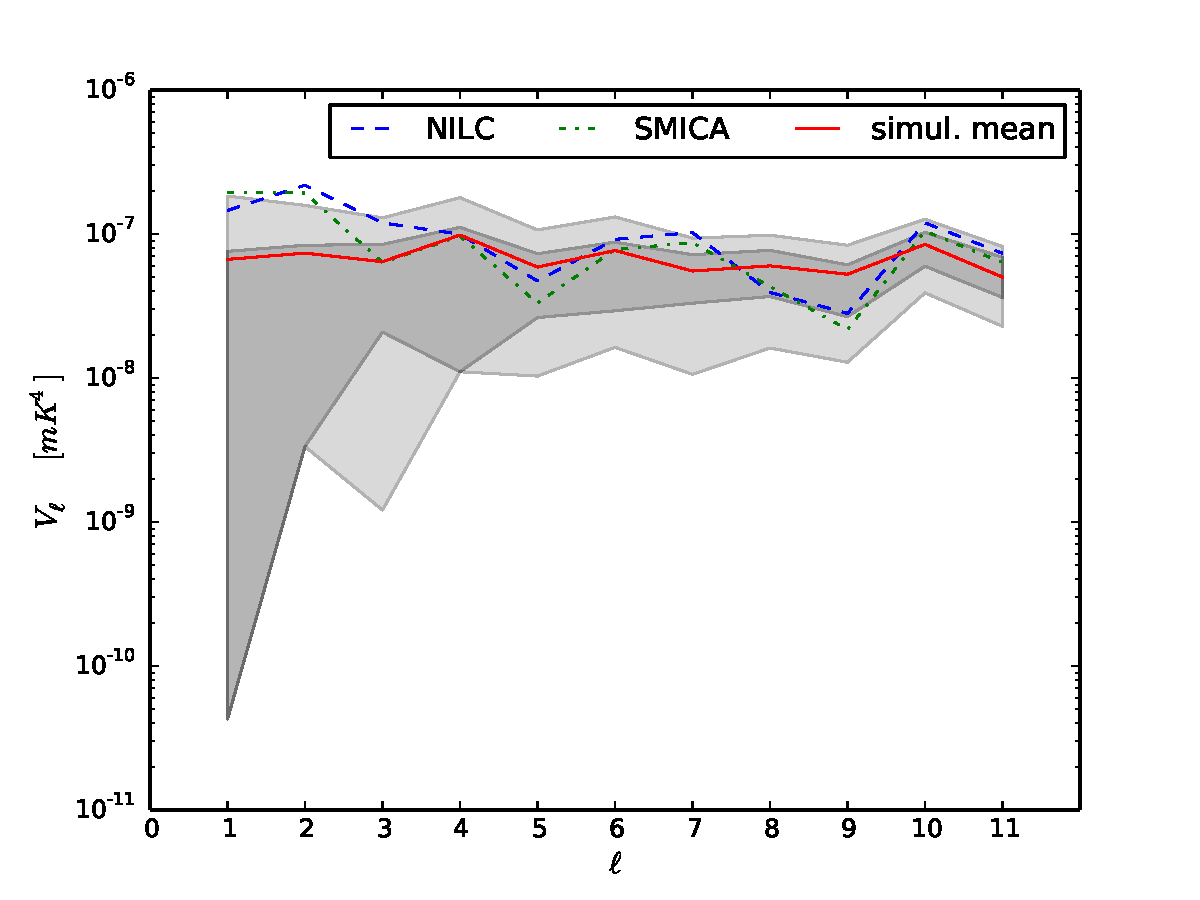
\includegraphics[scale=0.3]{figures/chapter-vsk/Inp_Vl.pdf}
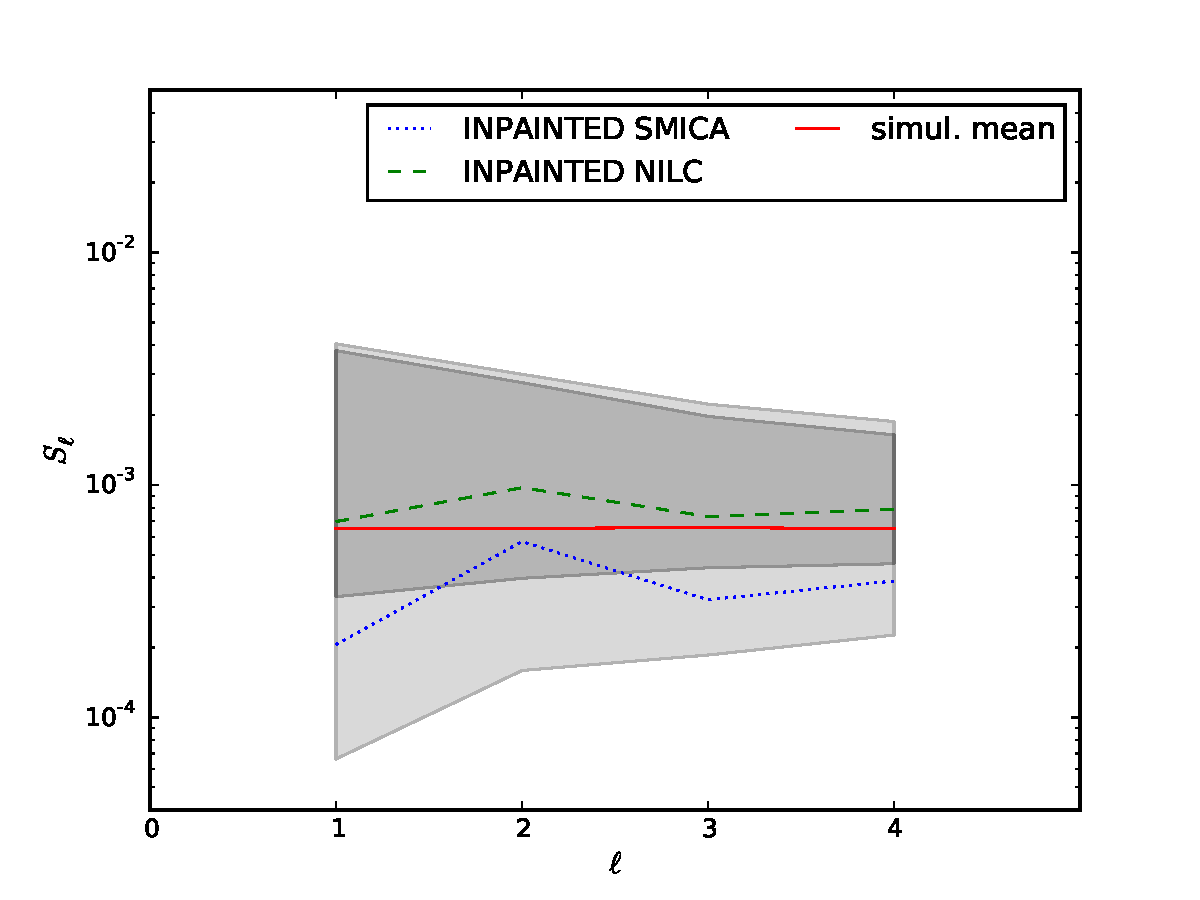
\includegraphics[scale=0.3]{figures/chapter-vsk/Inp_Sl.pdf}\\
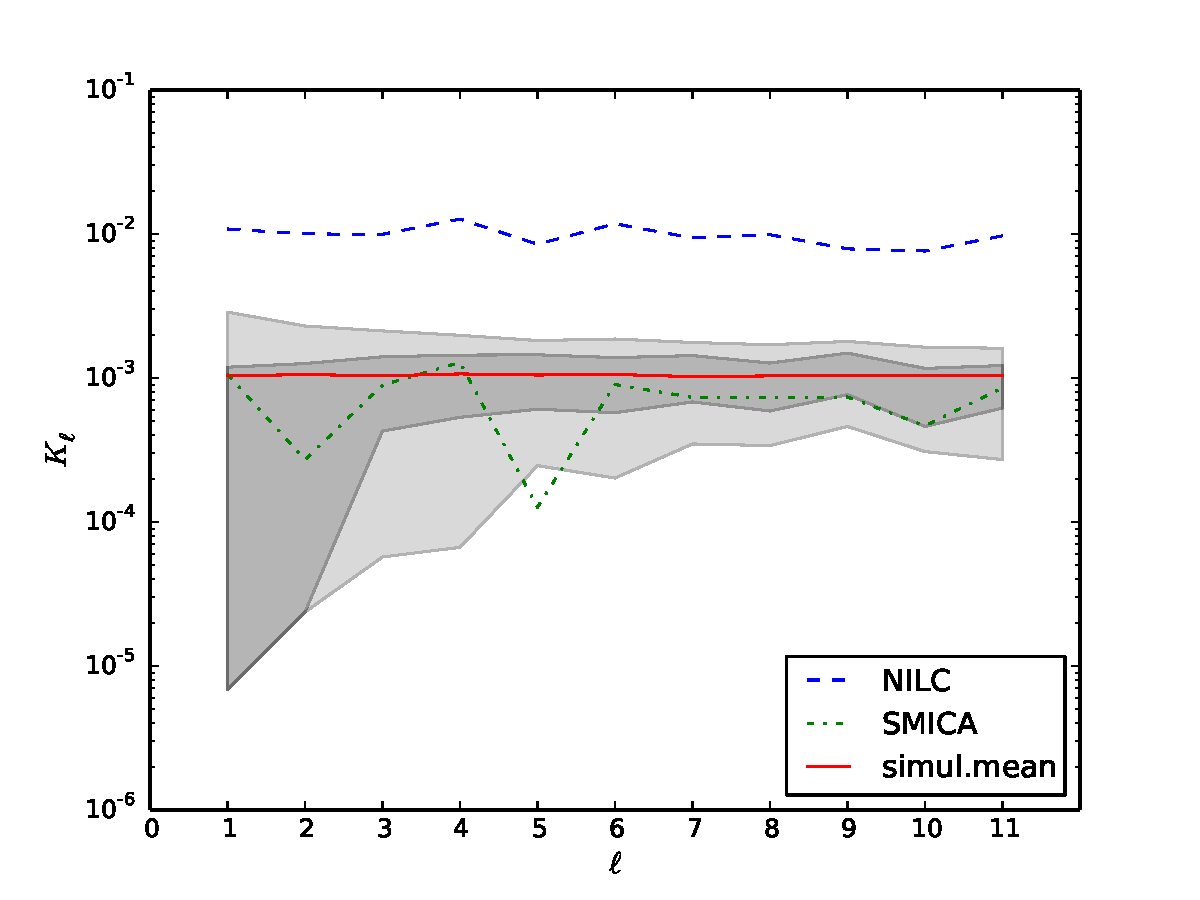
\includegraphics[scale=0.3]{figures/chapter-vsk/Inp_Kl.pdf}
\caption{Angular power spectra for the $N'_{side} = 4$ V-map, S-map, and K-map computed out of the full-sky $N_{side} = 2048$ inpainted CMB estimates. The red solid line indicates the mean for $1000$ Monte Carlo simulations and the shaded dark and light gray regions indicate the $68$ per cent and $95$ per cent confidence regions, respectively.}
\label{Fig:1}
\end{figure}

\begin{figure}
\centering
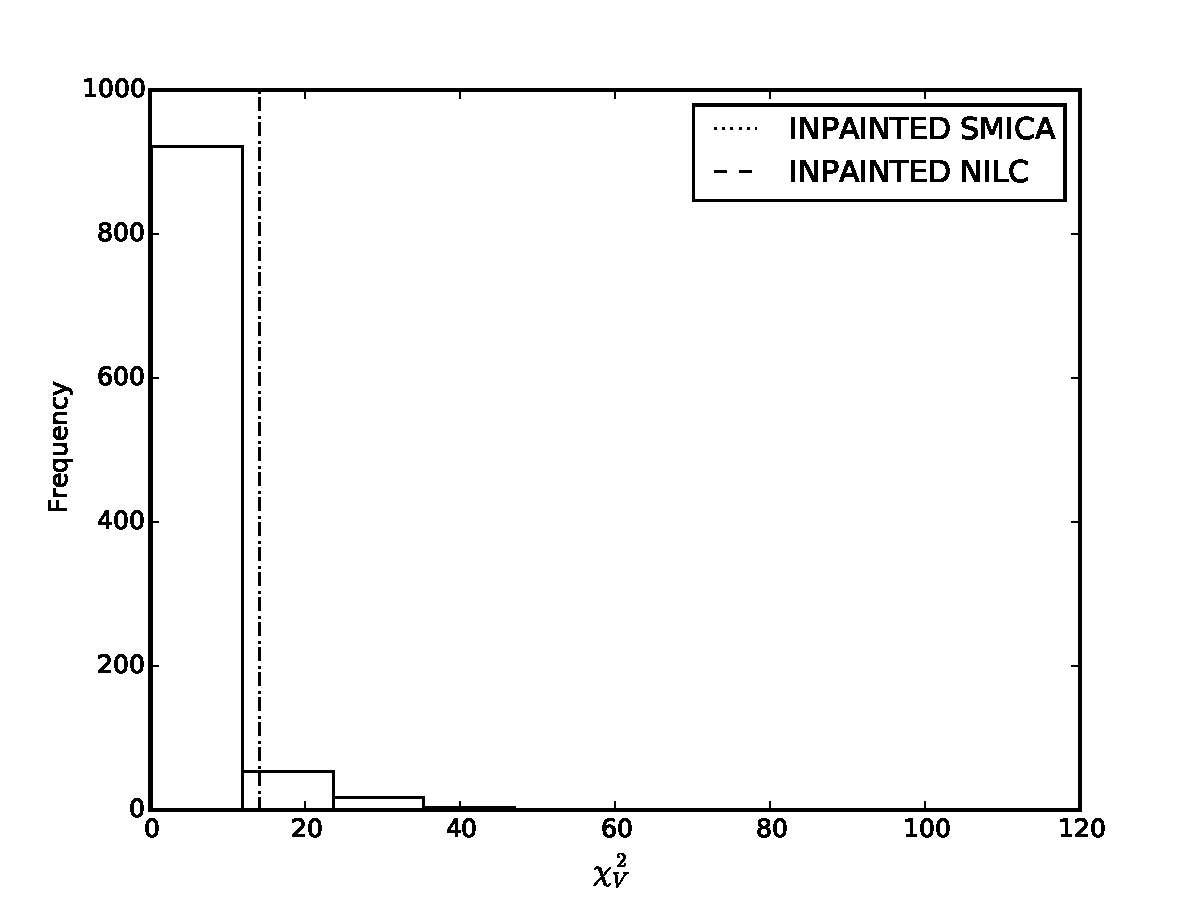
\includegraphics[scale=0.3]{figures/chapter-vsk/vchi2.pdf}
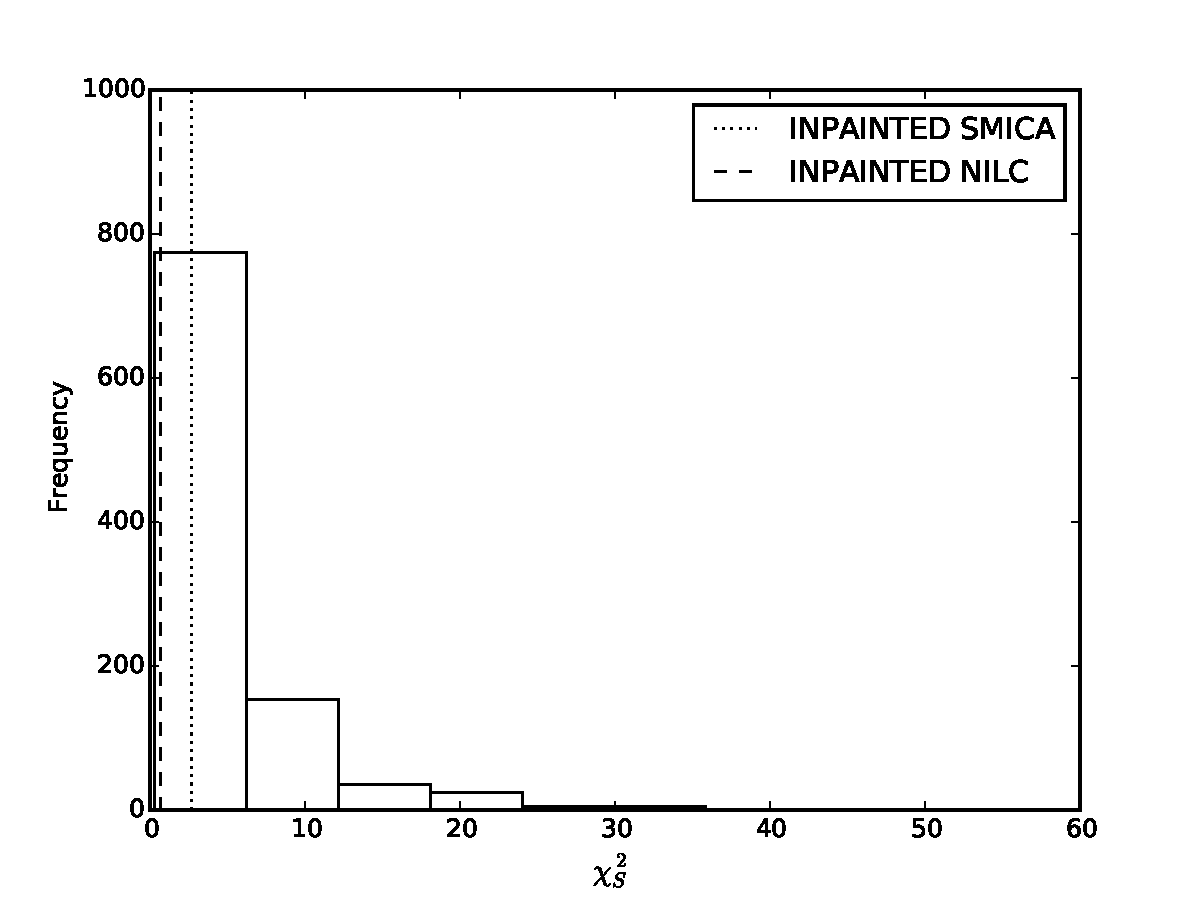
\includegraphics[scale=0.3]{figures/chapter-vsk/schi2.pdf}\\
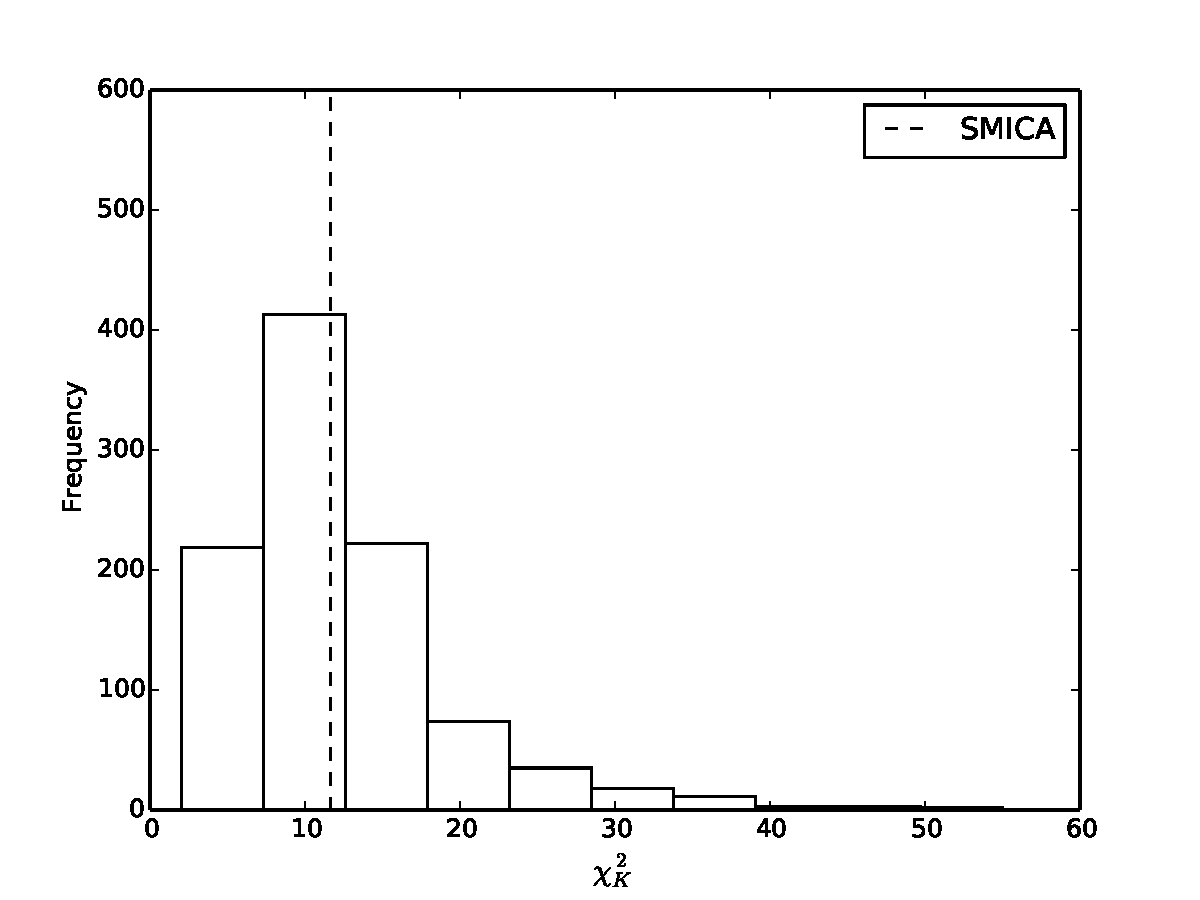
\includegraphics[scale=0.3]{figures/chapter-vsk/kchi2.pdf}
\caption{N-pdf $\chi^ 2$ for the angular power spectra shown in Fig. \ref{Fig:1}. The vertical lines show values for the corresponding CMB estimates.}
\label{Fig:2}
\end{figure}

\begin{table}
\centering
\caption{Lower-tail probability for the V, S, K estimators at different resolutions, for the $N_{side} = 2048$ inpainted \texttt{SMICA} and \texttt{NILC}.}
\label{table:1}
\begin{tabular}{@{}lcccc}
\hline 
  & & Probability & \\
\hline  
CMB estimate & V & S & K \\ 
\hline  
 & & $N'_{side}=2$ & \\
\texttt{SMICA} & $0.977$ & $0.355$ & $0.038$ \\ 
\texttt{NILC} & $0.972$ & $0.781$ & $1.0$  \\
 & & $ N'_{side} = 4 $ & \\
\texttt{SMICA} & $0.998$ & $0.718$ & $0.585$ \\
\texttt{NILC} & $0.985$ & $0.988$ & $1.0$ \\
 & & $N'_{side} = 8$ & \\
 \texttt{SMICA} & $1.0$ & $0.374$ & $0.745$ \\
 \texttt{NILC} & $0.995$ & $0.385$ & $1.0$ \\
 & & $N'_{side} = 16$ & \\
 \texttt{SMICA} & $1.0$ & $0.241$ & $0.786$ \\
 \texttt{NILC} & $1.0$ & $0.093$ & $1.0$ \\
\end{tabular} 
\end{table}

According to the previous analysis the inpainting technique applied to \texttt{NILC} might induce some deviations of the null hypothesis. Therefore we now apply the V-S-K method to the almost full-sky $N_{side}=2048$ CMB estimates. We examine the four component separation methods mentioned above and use the U73 mask. In Fig. \ref{Fig:3} we illustrate, as an example, the V-map, S-map, and the K-map for the \texttt{SMICA} estimate. In Fig. \ref{Fig:4} we plot the corresponding angular power spectra $V_{\ell},\, S_{\ell},\, $ and $K_{\ell}$ computed for the four component separation CMB estimates. As can be seen, all the four estimates seem to be consistent with the null hypothesis. Nevertheless, note that due to the masked regions in the V-maps, S-maps, and K-maps the angular power spectra of the simulations are not any longer scale independent, the effect being much more visible in the case of $V_{\ell}$ because of the much more different value associated with the masked pixels. A possible modification in the method to include only unmasked regions in the computation of the angular power spectrum would be necessary to avoid these spurious features. Nevertheless, since in this work we want to test whether or not the \textit{Planck} data are consistent with the null hypothesis, we will not include  this modification in the present paper. Such a modification would require to adapt the V-S-K method as explained in \cite{Gorski1994} and \cite{Hivon2002}.

Comparing the results of the full-sky inpainted CMB maps with those of the almost full-sky CMB maps, we can see that there is no departure from the null hypothesis in the NILC CMB estimate when the inpainted regions are disregarded. Thus, the discrepancy observed in the full-sky map for the K estimator seems to be caused by the inpainted regions in the inpainted \texttt{NILC}. The four component separation methods exhibit a dipole in the V-maps outside the $95$ per cent confidence region for $N'_{side}=2$, but this feature disappears gradually  when increasing the parameter $N'_{side}$. This might be due to the fact that by construction the method V-S-K, as we have applied it here, disregards patches (patches set to zero) with less than $80$ per cent of unmasked pixels and therefore it is not guaranteed that the sky fraction (fraction of the sky having patches with non zero value) be the same for each $N'_{side}$. 

Since all the four component separation methods give pretty similar results and to avoid circumlocution, in Table \ref{table:2} we present the lower-tail probabilities only for the \texttt{SMICA} CMB estimate. We have examined the dependence of our results on the parameters $N_{side}$ and $N'_{side}$. In summary, we do not see significant deviation of the null hypothesis for almost all the possible combinations of parameters considered, with the exception of the V estimator for $N_{side}=2048$ and $N'_{side}=8,\,16$ where there is a discrepancy with the simulations.
 

\begin{figure}
\centering
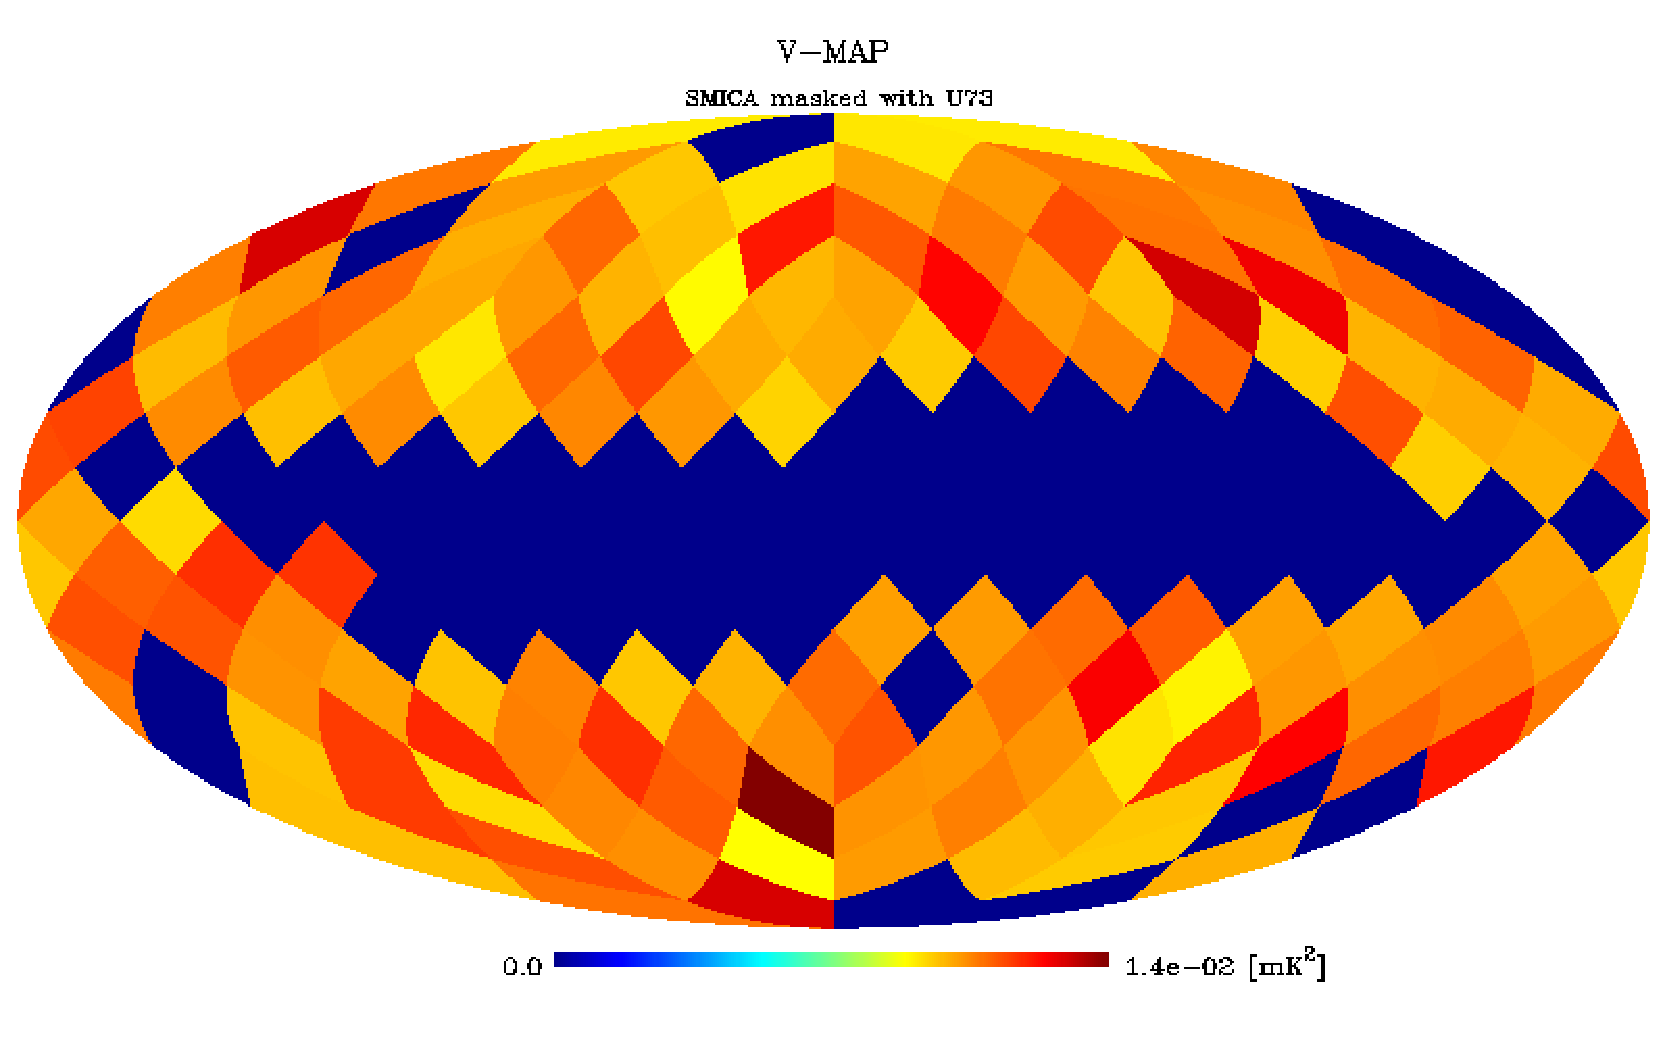
\includegraphics[scale=0.3]{figures/chapter-vsk/vmap.pdf}\\
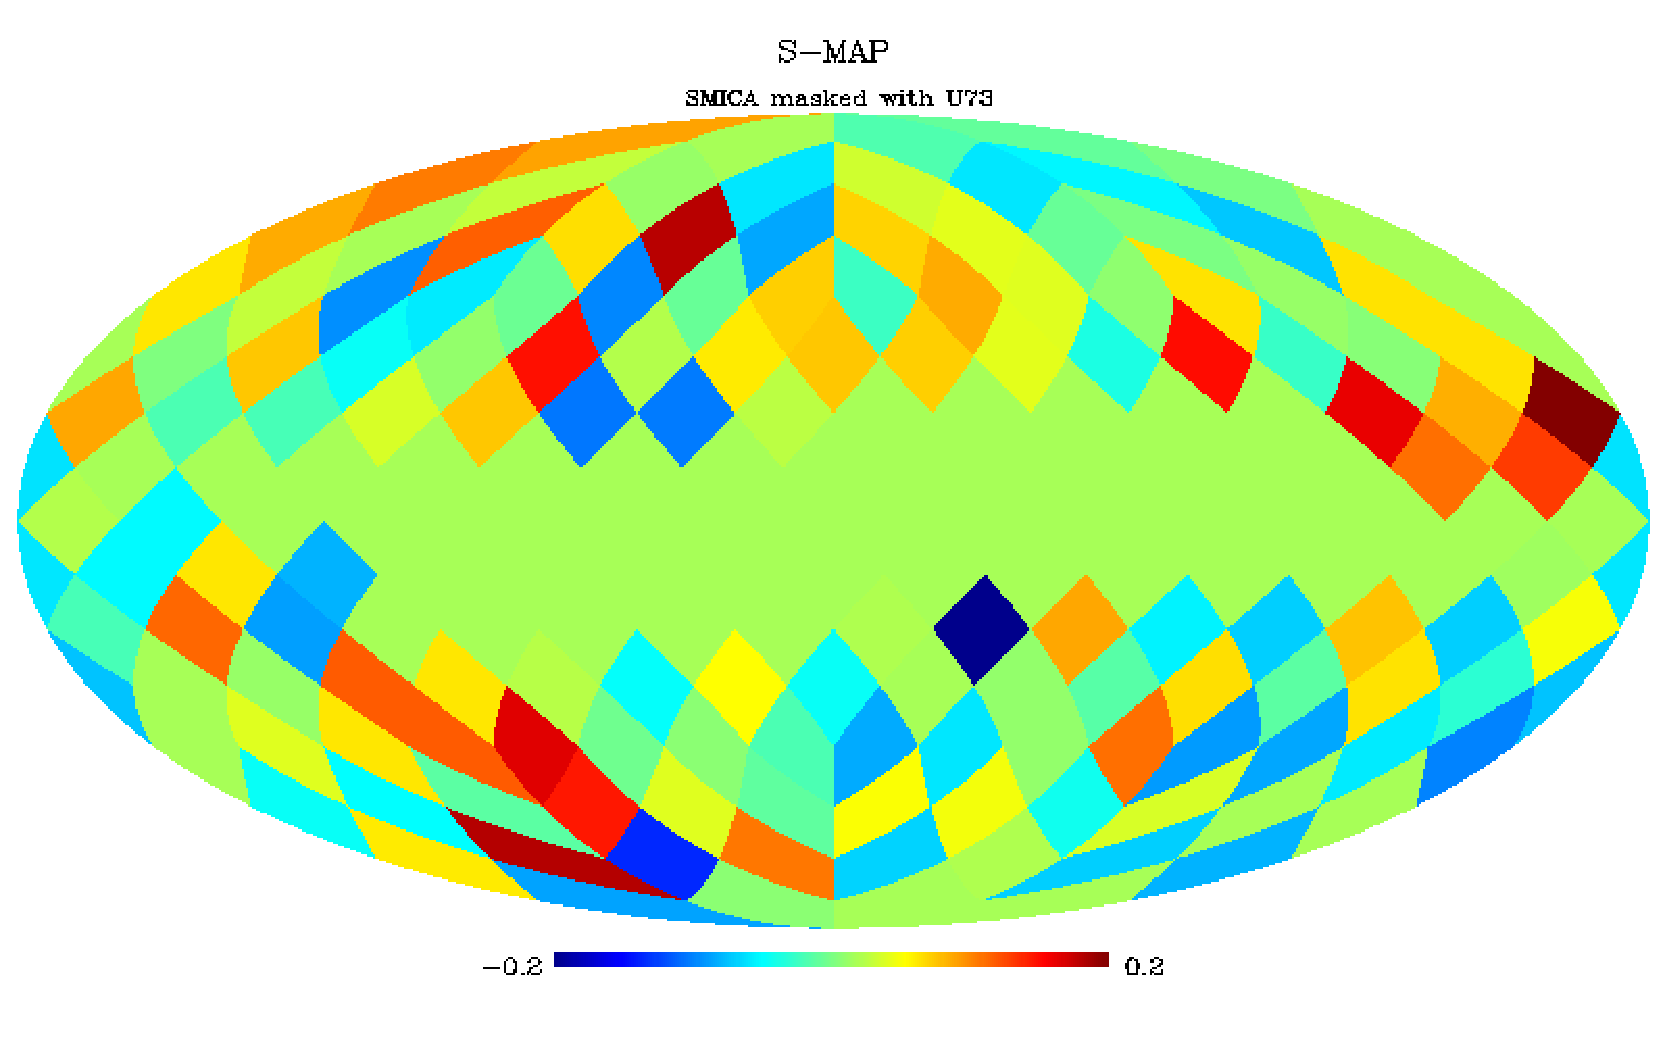
\includegraphics[scale=0.3]{figures/chapter-vsk/smap.pdf}\\
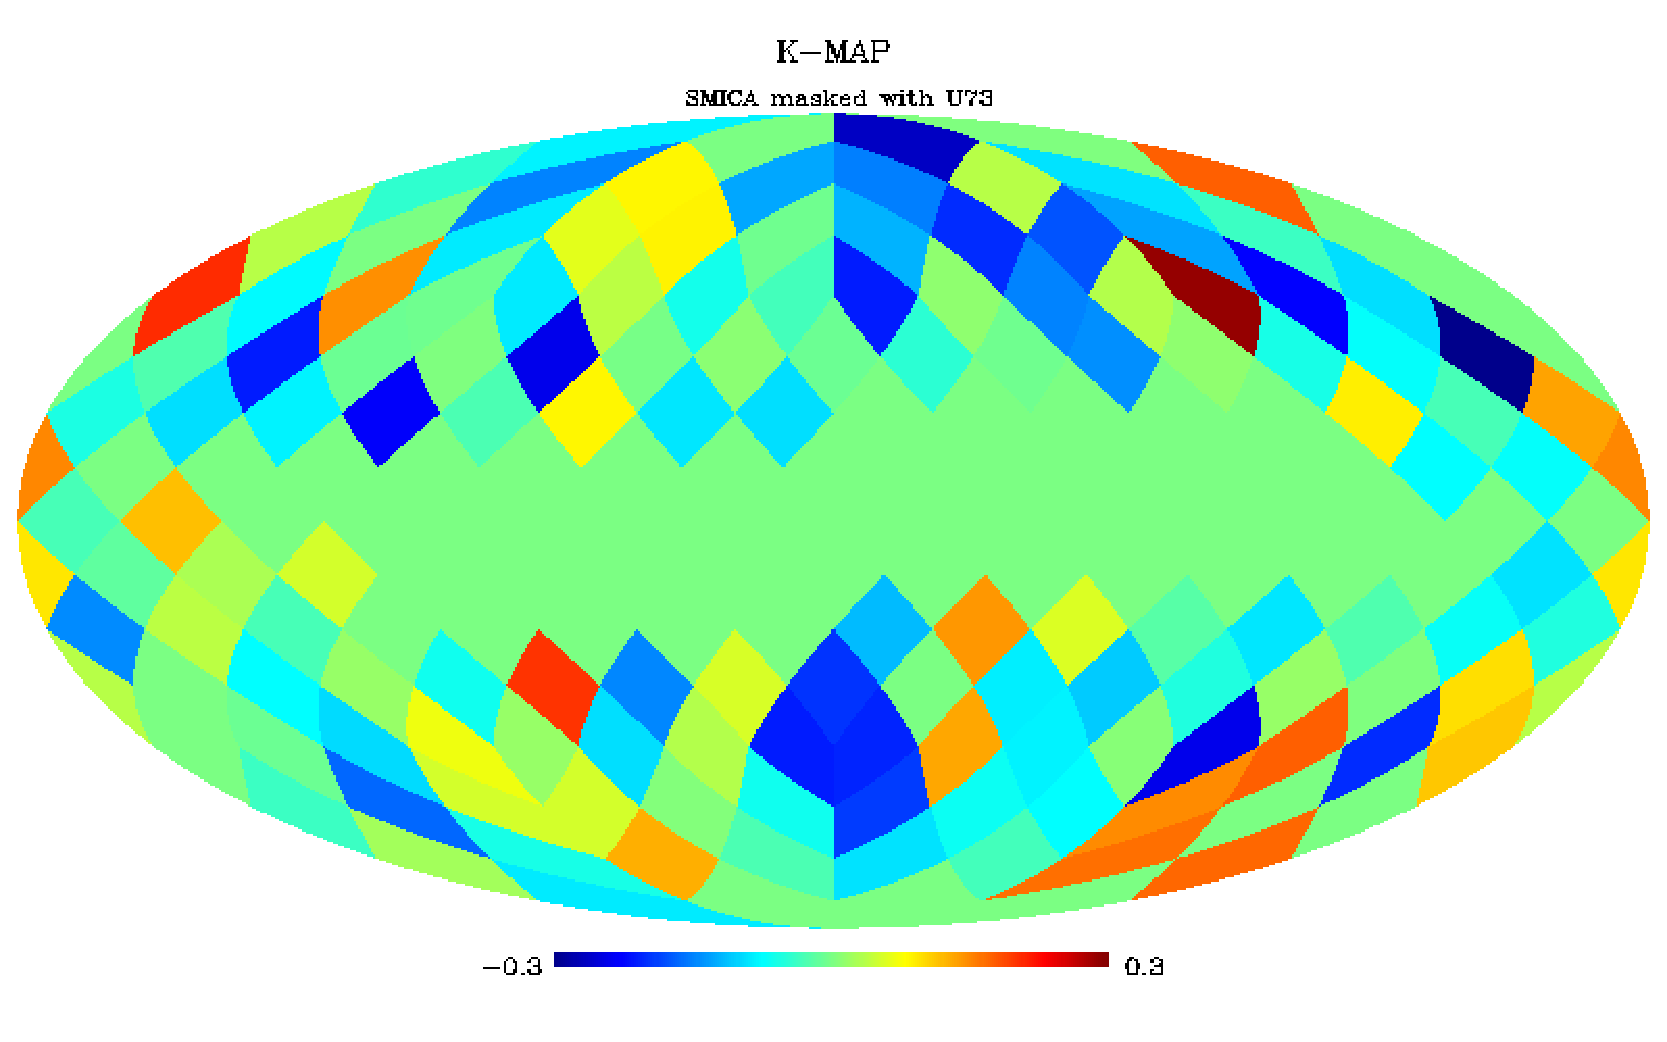
\includegraphics[scale=0.3]{figures/chapter-vsk/kmap.pdf}
\caption{$N'_{side = 4}$ V-map (\textit{upper}), S-map (\textit{middle}), and K-map (\textit{lower}) for the $N_{side} = 2048$ SMICA CMB estimate masked with the U73 mask.}
\label{Fig:3}
\end{figure}

\begin{figure}
\centering
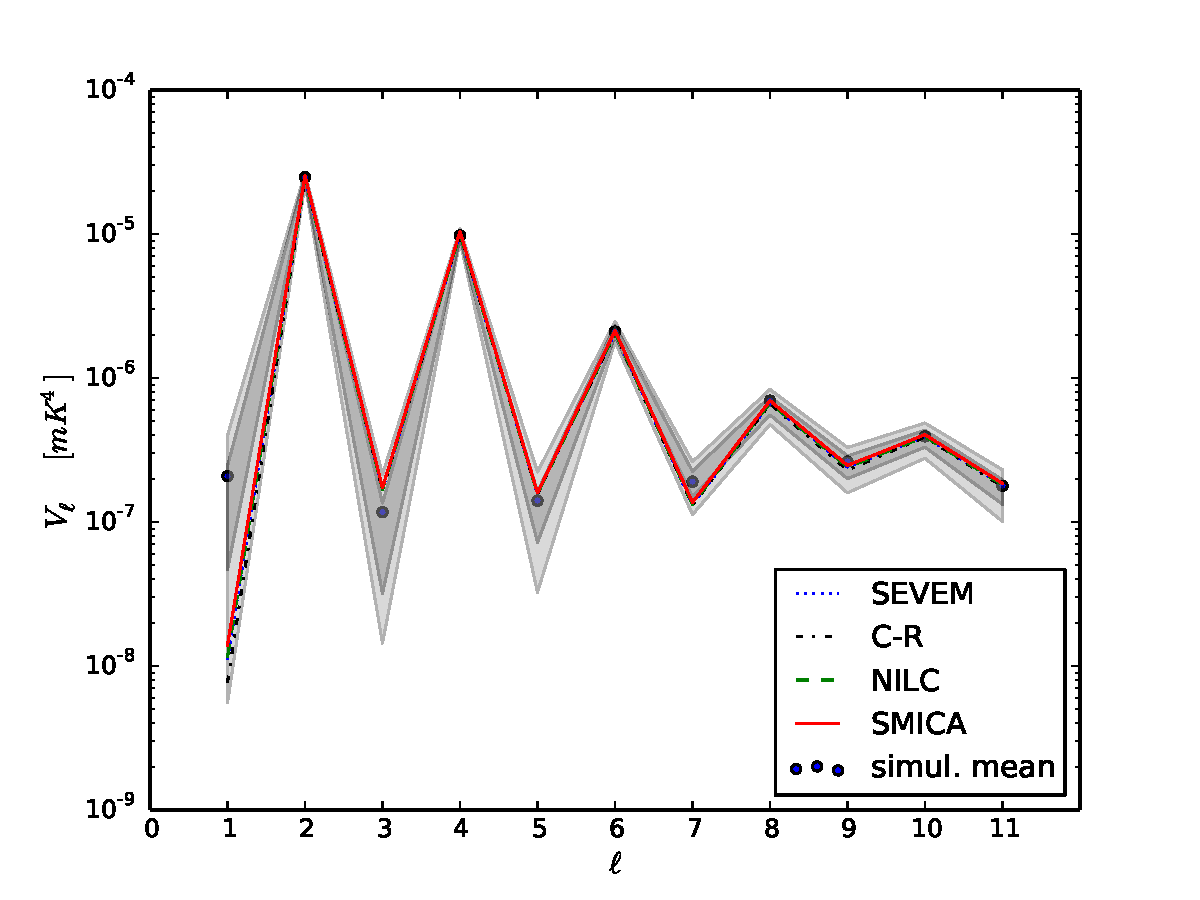
\includegraphics[scale=0.3]{figures/chapter-vsk/Vl_u73.pdf}
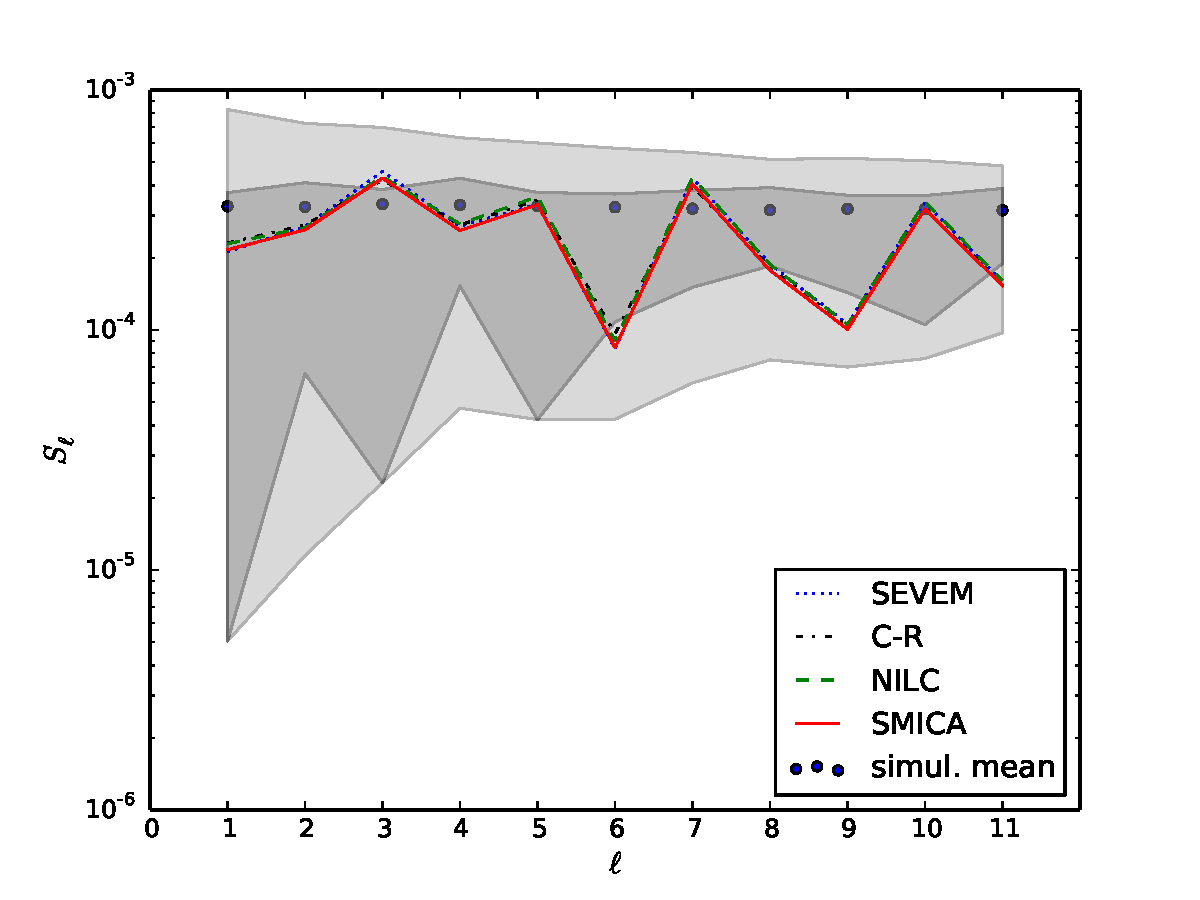
\includegraphics[scale=0.3]{figures/chapter-vsk/Sl_u73.pdf}\\
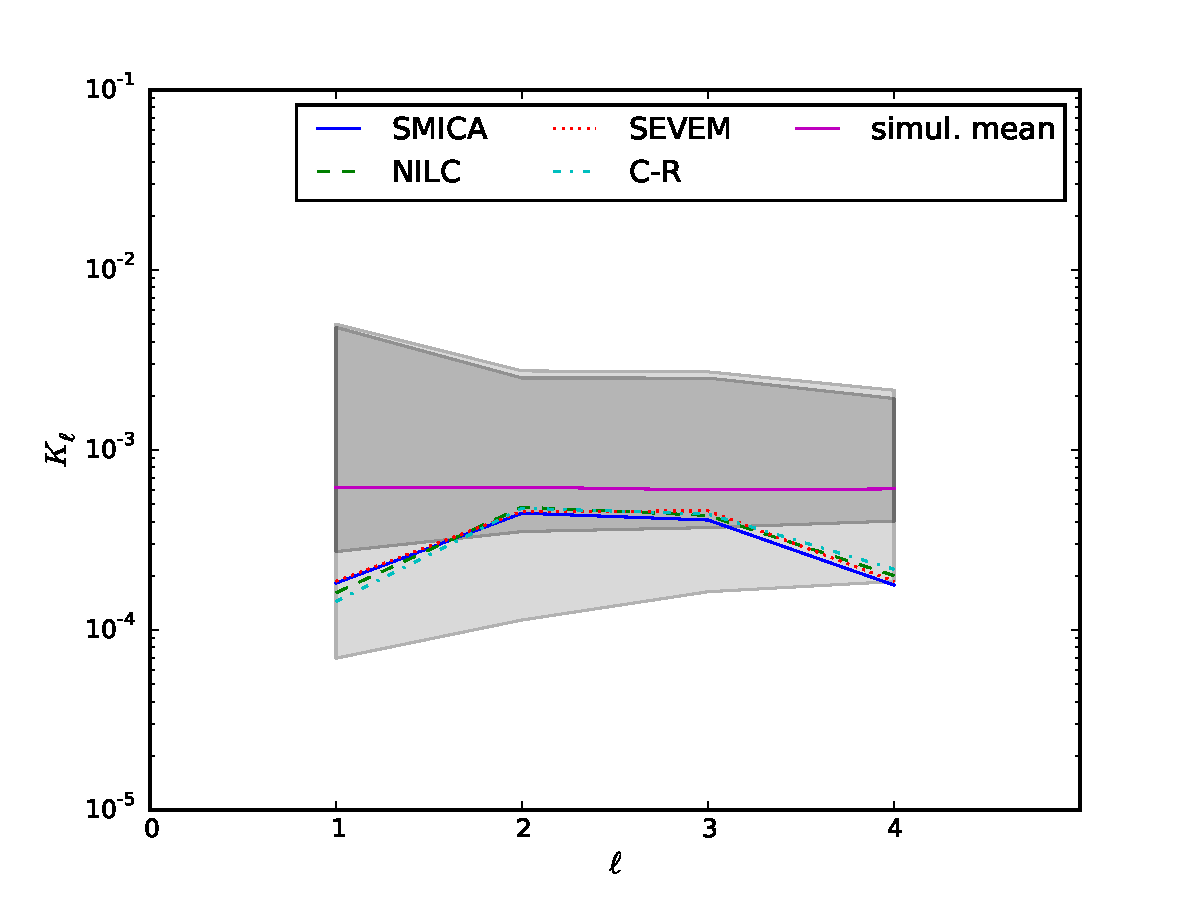
\includegraphics[scale=0.3]{figures/chapter-vsk/Kl_u73.pdf}
\caption{Angular power spectra of the $N'_{side} = 4$ V-map, S-map, and K-map for the four $N_{side} = 2048$ CMB estimates. The blue dots indicate the mean angular power spectrum for $1000$ Monte Carlo simulations and the shaded dark and light gray regions indicate the $68$ per cent and $95$ per cent confidence regions, respectively.}
\label{Fig:4}
\end{figure}

We have also studied the mask dependence of the V-S-K method. The results for both the confidence mask and the mask of inpainted regions for \texttt{SMICA} are shown in Table \ref{table:3}. In order to facilitate the comparison some of the results for the mask U73 are repeated. The sky coverage of the considered masks does not seem to affect the results considerably in any of the estimators. 

\begin{table}
\centering
\caption{Lower-tail probability for the V, S, K estimators at different resolutions $N'_{side}$, for different resolutions $N_{side}$ of the  \texttt{SMICA} CMB estimate using the U73 mask.}
\label{table:2}
\begin{tabular}{@{}lcccc}
\hline 
  & & Probability & \\
\hline  
$N'_{side}$ & V & S & K \\ 
\hline  
 & & $N_{side}=2048$ & \\
$2$ & $0.929 $ & $ 0.152$ & $0.513 $ \\ 
$4$ & $ 0.754$ & $0.656 $ & $0.292 $  \\
$8$ & $ 1.0$ & $ 0.094 $ & $ 0.412 $  \\
$16$ & $ 1.0 $ & $ 0.391 $ & $ 0.439 $  \\
 & & $ N_{side} = 1024 $ & \\
$2$ & $ 0.869 $ & $ 0.151 $ & $ 0.523 $ \\ 
$4$ & $ 0.394 $ & $ 0.653 $ & $ 0.253 $  \\
$8$ & $ 0.835 $ & $ 0.145 $ & $ 0.457 $  \\
$16$ & $ 0.928 $ & $ 0.226 $ & $ 0.265 $  \\
 & & $N_{side} = 512$ & \\
$2$ & $0.273 $ & $ 0.174 $ & $ 0.626 $ \\ 
$4$ & $ 0.532 $ & $ 0.651 $ & $ 0.195 $  \\
$8$ & $ 0.5 $ & $ 0.167 $ & $ 0.559 $  \\
$16$ & $ 0.492 $ & $ 0.231 $ & $ 0.331 $  \\
 & & $N_{side} = 256$ & \\
$2$ & $ 0.276 $ & $ 0.235 $ & $ 0.647 $ \\ 
$4$ & $ 0.393 $ & $ 0.571 $ & $ 0.232 $  \\
$8$ & $ 0.192 $ & $ 0.216 $ & $ 0.518 $  \\
$16$ & $ 0.589$ & $ 0.176 $ & $ 0.409 $  \\
\end{tabular} 
\end{table}

\begin{table}
\centering
\caption{Lower-tail probability for the V, S, K estimators at different resolutions $N'_{side}$, for the \texttt{SMICA} CMB estimate using different masks.}
\label{table:3}
\begin{tabular}{@{}lcccc}
\hline 
  & & Probability & \\
\hline  
$N'_{side}$ & V & S & K \\ 
\hline  
 & & U73 & \\
$2$ & $ 0.929 $ & $ 0.152 $ & $ 0.513 $ \\ 
$4$ & $ 0.754 $ & $ 0.656 $ & $ 0.292 $  \\
 & & VALMASK & \\
$2$ & $ 0.983 $ & $ 0.388 $ & $ 0.423 $ \\ 
$4$ & $ 0.741 $ & $ 0.754 $ & $ 0.319 $  \\
 & & INP$\_$MASK & \\
$2$ & $ 0.976 $ & $ 0.37 $ & $ 0.163 $ \\ 
$4$ & $ 0.996 $ & $ 0.738 $ & $ 0.528 $  \\
\end{tabular} 
\end{table}


\section{Summary}
\label{s:summary}

In this work we have applied a non-parametric analysis, the V-S-K method, to test for possible departures from the cosmological principle in the CMB anisotropies measured by the \textit{Planck} satellite. We have used the available full-sky maps (inpainted \texttt{SMICA} and \texttt{NILC}) and the four almost full-sky CMB estimates released by the \textit{Planck} collaboration (\texttt{SMICA, NILC, Commander-Ruler,} and \texttt{SEVEM}) to investigate possible anomalous angular variations of the variance, skewness, and kurtosis in the CMB anisotropies. We have determined the statistical significance of our results by using a set of Gaussian, isotropic simulations of the CMB sky seeded by the \textit{Planck} best-fit angular power spectrum.    

The V-S-K method applied to inpainted \textit{Planck} maps brings out the following features. The V estimator measures departure ($95$ per cent confidence region) of the null hypothesis at the level of the dipole and the quadrupole which are robust against both component separation and the parameter $ N'_{side} $ of the V-S-K method. The S estimator is fully consistent with the null hypothesis in both CMB estimates. This is not the case for the K estimator, where only inpainted \texttt{SMICA} turns out to be consistent with the simulations. According to the K estimator, the inpainting method applied to \texttt{NILC } seems to induce kurtosis at all scales allowed by a given $ N'_{side} $. However, this discrepancy with the null hypothesis becomes  less significant when higher $ N'_{side} $ are employed. 

Next, we have studied several aspects of the V-S-K method applied to the almost full-sky \textit{Planck} maps. In particular, we have considered the V-S-K method applied to the four component separation CMB estimates by using different resolutions of the data ($ N_{side} $), masks, and $ N'_{side} $. All the four component separation methods are fully consistent with the hypothesis of a universe statistically isotropic and Gaussian regardless of those parameters of the V-S-K method. 

When applying the V-S-K method to masked CMB maps one must be careful. Since the method computes the full-sky angular power spectrum of V-map, S-map, and K-map, the masked region of those maps might include strong angular variations if the value of the unmasked pixels is very different from the masked ones.  A modified V-S-K method should take into account only unmasked pixels of the V-map, S-map, and K-map in order to avoid this caveat. Since both the simulations and the data are affected in the same way by this limitation of the method, such modification would not alter our results (consistency with the null hypothesis), but produce the true form of the angular power spectra. 

Finally, we notice that although our results are compatible with most of the analysis done by the \textit{Planck} team, a direct comparison is not possible. First, by construction, the V-S-K method may not use the same fraction of the sky as analysed by some of the statistical methods used by the \textit{Planck} team. Second, we do not use the sophisticated set  of Gaussian, isotropic simulations  (the FFP6 simulations) employed by the \textit{Planck} team in their analysis. 


\chapter{Traces of dark energy anisotropic stress}
\label{chapter-ade}

\section{Introduction}
\label{chapter-ade:introduction}

The last twenty years have witnessed a revolution in observational cosmology, with 
an incredible growth of data available to cosmologists. When interpreted within 
the cosmological standard model, one consequence of the observations is the need 
for an accelerated expansion of the Universe. To drive this acceleration a new 
constituent is required, called dark energy. The main candidate model for the dark 
energy is the cosmological constant $\Lambda$, but this model suffers from severe 
fine-tuning issues. Even though cosmologists have been very active and have 
invented a large number of other possible models, including modifications to 
general relativity as the theory of gravity, none of them appear like natural 
candidates for the dark energy (see e.g.\ \cite{Copeland:2006wr, Durrer:2008in, 
Frieman:2008sn, Amendola2010, Clifton:2011jh, Amendola:2012ys} for reviews).

The jury is therefore still out concerning the nature of the dark energy, and it 
may be preferable to approach the problem from the observational side, by 
characterising the possible observational consequences of the dark energy, and 
then investigating the link between those and its physical nature. (See e.g.\ 
\cite{Kunz:2012aw} for a short review, as well as \cite{Battye:2012eu, 
Sawicki:2012re, Baker:2012zs, Gubitosi:2012hu, Bloomfield:2012ff} for recent 
works on parameterised or effective action approaches.)

Useful quantities that are close to the observations are the functions that 
describe the metric \cite{Amendola:2007rr, Hu:2007pj, Sawicki:2012re, 
Amendola:2012ky, Motta:2013cwa}. If we only use quantities up to first order in
perturbation theory, and keep only scalar perturbations, then the metric can be 
written as
\begin{equation}
g_{\mu\nu}dx^\mu dx^\nu = a^2\left\lbrace -\(1+2\psi\)\,d\eta^2
  + \(1-2\phi\)\,\delta_{ij} dx^i dx^j \right\rbrace\,, \label{eq:metric}
\end{equation}
where we used the longitudinal gauge. The relevant quantities then are the scale 
factor $a(\eta)$, or equivalently the Hubble parameter $H(\eta)$, and the two 
gravitational potentials $\phi(k,\eta)$ and $\psi(k,\eta)$. The evolution of the 
Hubble parameter is measured by probes like the luminosity distance to type-Ia 
supernovae (SN-Ia) or the baryonic acoustic oscillations (BAO). Possible probes of 
the gravitational potentials include weak lensing which measures the integral of 
$\phi+\psi$, the motion of test particles which is governed by $\psi$ or also the 
integrated Sachs-Wolfe (ISW) effect of the cosmic microwave background (CMB) or 
the large-scale distribution of galaxies.

The standard dynamical dark energy model invokes an additional minimally coupled scalar 
field, possibly with a non-canonical kinetic term. An important feature of this 
class of models is that the scalar field does not support any anisotropic stress 
in linear theory, i.e.\ the space-space part of its energy-momentum tensor has only a 
trace contribution. So-called modified-gravity models, which include 
scalar-tensor, $f(R)$, brane-world and similar models, generically have a non-zero 
(effective) contribution to the anisotropic stress. As a non-zero anisotropic 
stress manifests itself through a gravitational slip, $\phi\neq\psi$, the 
effective anisotropic stress provides a crucial observational test for the nature 
of the dark energy \cite{Kunz:2006ca, Saltas:2010tt}.

Much of the effort in the literature has so far focused on determining 
observational bounds on the background evolution, usually for scalar field models 
without anisotropic stress (e.g.\ \cite{Copeland:2006wr, Frieman:2008sn,Sapone:2010iz,Amendola:2012ys}). 
In this paper we will investigate specifically how a non-zero 
anisotropic stress impacts the dark energy and dark matter perturbations, as well 
as the CMB. For this, we use phenomenological prescriptions that are 
motivated by the typical behaviour of the anisotropic stress for a range of 
modified gravity models. We focus on two model ingredients: externally and 
internally sourced anisotropic stress which reflects a simplified version of a 
more general structure proposed in \cite{Sawicki:2012re}. The paper is structured 
as follows: in the next section we briefly present the perturbation equations 
including anisotropic stress, which also serves to define our notation, as well as 
our closure relations for the pressure perturbations and the dark energy 
anisotropic stress. We then study the phenomenological impact of the presence of a 
nonzero anisotropic stress in section 3, before discussing observational 
constraints from the CMB and geometrical probes in section 4. In section 5 we 
relate the effect of the anisotropic stress to the `modified growth' 
parameterisations that are commonly used in the literature.  We finally conclude 
in section 6. The appendices contain more detailed explanations for the stability 
analysis as well as some exact but cumbersome solutions of the perturbation 
evolution.

\section{Models of anisotropic dark energy}
\label{chapter-ade:models}

\subsection{Perturbation equations}

We have already given the perturbed metric in longitudinal gauge in Eq.\ 
(\ref{eq:metric}). A prime will stand for the derivative w.r.t.\ conformal time, 
$\eta$, and $\H\equiv a'/a=aH$ is the comoving Hubble parameter while $H$ is the 
physical Hubble parameter that takes the value of the Hubble constant $H_0$ today 
when $a_0=1$. The continuity and Euler equations for the dark energy 
perturbations read \cite{Bardeen:1980kt, Kodama:1985bj, Ma:1995ey}
\be
\delta'_{de} +3\H\(\frac{\delta P_{de}}{\rho_{de}}-w\delta_{de}\)
  +(1+w)kv_{de}  -3(1+w)\phi'  =  0
\label{eq:de-cont}
\\
v_{de}' +\H(1-3c_a^2)v_{de} -k\( \psi +\frac{\delta P_{de}}{(1+w)\rho_{de}}
-\frac{2\pi_{de}}{3(1+w)} \)  =  0
\label{eq:de-eul}
\ee
where the adiabatic sound speed is
\be
  c_a^2  \equiv  \frac{P_{de}'}{\rho_{de}'}  =  w - \frac{w'}{3\H(1+w)} \,.
\ee
The evolution equations for the dark matter are the same, but with 
$w_m=\delta P_m = \pi_m = 0$. Notice that in terms of the often used variable 
$\sigma$ for the anisotropic stress \cite{Ma:1995ey} we have that 
$\pi = (3/2)(1+w)\,\sigma$.


In addition to these evolution equations we need the Einstein constraint 
equations to compute the impact of the dark matter and dark energy perturbations 
on the metric. For the scalar perturbations considered here, there are two 
independent Einstein equations which we can take to be
\be
- k^2 \phi &=& 4 \pi G a^2 \left(\rho_m \Delta_m + \rho_{de} \Delta_{de} \right) 
\, , \label{eq:poisson} \\
k^2 (\phi - \psi) &=& 8 \pi G a^2 \rho_{de} \pi_{de} \, . \label{eq:aniso}
\ee
Here we wrote the Poisson equation (\ref{eq:poisson}) directly in terms of the 
comoving density perturbation $\Delta$ which is linked to the density 
perturbation in the longitudinal gauge $\delta$ by a gauge transformation, 
$\Delta = \delta + 3 \H (1+w) v/k$. In the equation for the slip (\ref{eq:aniso}) 
we further used that $\pi_m = 0$ (which is strictly speaking only true at first 
order in perturbation theory \cite{Ballesteros:2011cm}). From the two equations 
(\ref{eq:de-cont}) and (\ref{eq:de-eul}) one can derive a single second order 
evolution equation for $\delta_{de}$ by solving the continuity equation 
(\ref{eq:de-cont}) for $v_{de}$ and substituting that (and its derivative) into 
the Euler equation (\ref{eq:de-eul}). We find
\bea
  \delta''_{de} &+&\(1-6w\) \H \delta'_{de}
    +3 \H \(\!\frac{\delta P_{de}}{\rho_{de}}\!\)'
    +3 \Big[(1-3w)\H^2+\H'\Big] \(\frac{\delta P_{de}}{\rho_{de}}-w\delta_{de}\) \nonumber \\
    &-&3 \H w' \delta_{de}
%\nonumber \\
 = 3(1+w)\[\phi'' + \(1-3w +\frac{w'}{(1+w)\H}\) \H \phi' \] \nonumber \\
    &-& k^2\[ (1+w)\psi + \frac{\delta P_{de}}{\rho_{de}} -\frac{2}{3}\pi_{de} \] 
\,.
\label{eq:de-secondorder}
\eea
To this point we did not make any assumptions on $\delta P_{de}$, $\pi_{de}$ and 
$w$. However, already the last term makes clear that $k^2\pi_{de}$ acts as a 
source for $\delta_{de}$ while the pressure counteracts the gravitational 
collapse. $-k^2\psi$ is also a source because $\psi=\phi$ for vanishing 
anisotropic stresses and $-k^2\phi\propto \H^2\Delta_{tot}$.



%%%%%%%%%%%%%%%%%%%%%%%%%%%%%%%%%%%%%%%%%%%%%%%%%%%%%%%%%%%%%%%%%%%%%%%%%%%%%%%%%
\subsection{Modelling the DE pressure perturbation}

We define the effective, non-adiabatic sound speed of DE in its rest-frame, 
$\partial_\mu P_{de}\equiv c_s^2 \partial_\mu \rho_{de}$. This is the form of 
the sound speed that e.g.\ $K$-essence type models exhibit, with $c_s^2=1$ for a 
canonical scalar field. When we perform a gauge transformation to the 
longitudinal gauge, we find
\be
\frac{\delta P_{de}}{\rho_{de}} = c_s^2\delta_{de} +3(1+w)\(c_s^2 - c_a^2\) 
    k^{-1}\H v_{de} \,. \label{eq:dp}
\ee
We keep the sound speed $c_s$ as a free parameter, but assume it to be a 
constant.




%%%%%%%%%%%%%%%%%%%%%%%%%%%%%%%%%%%%%%%%%%%%%%%%%%%%%%%%%%%%%%%%%%%%%%%%%%%%%%%%%
\subsection{Model 1: externally sourced anisotropic stress}

In the quasi-static limit of DGP, the metric potentials are directly linked to 
the matter  perturbations through a time-dependent function \cite{Koyama:2005kd} 
and consequently also the anisotropic stress is proportional to $\Delta_m$ 
\cite{Kunz:2006ca} with, in general, a time-dependent coefficient. Another 
motivation to link the dark energy anisotropic stress to the matter is the 
possibility of couplings between dark energy and dark matter. To keep the model 
simple we use
\be
  \pi_{de}\ \equiv\  \aa a^n \Delta_m
\label{eq:model:1}
\ee
with a constant coefficient $\aa$. We will see that this term will act as an 
additional source for $\delta_{de}$. When looking at the constraints from 
data in section \ref{chapter-ade:constraints} we will fix $n=0$, which is also roughly the behaviour of the effective
anisotropic stress in the DGP model.



%%%%%%%%%%%%%%%%%%%%%%%%%%%%%%%%%%%%%%%%%%%%%%%%%%%%%%%%%%%%%%%%%%%%%%%%%%%%%%%%%
\subsection{Model 2: counteracting the pressure perturbation}

In \cite{Song:2010rm} a coupling of the anisotropic stress to the pressure 
perturbation was proposed, $\sigma \propto \delta P_{de}/\rho_{de}$, linking 
isotropic and anisotropic stresses which appears quite natural\footnote{A similar 
link was also exploited in \cite{Kunz:2006ca} to define the pressure perturbation when mimicking DGP.}. For non-zero sound 
speed the pressure perturbation is related to the density perturbation by our 
model (\ref{eq:dp}). Here we formulate the dependence directly in terms of the 
comoving density perturbation since this is a gauge-invariant prescription. In 
addition, we allow for a different behaviour on small and large scales, with a 
transition scale $k_T$
\be
\pi_{de}\ = \ff \frac{(k/k_T)^2}{1+(k/k_T)^2} \Delta_{de} \quad , \, k_T = \gg
\H(a)
\ee
with constant parameters $\ff$ and $\gg$. We can then write this model also as
\be
\pi_{de}\ = \frac{\ff}{1 +(\gg\H/k)^2} \Delta_{de} \, .
\label{eq:model2}
\ee
For $\ff = (3/2) c_s^2$ the anisotropic stress cancels the pressure perturbation 
in the Euler equation (\ref{eq:de-eul}) on sub-horizon scales, but not in the 
continuity equation (\ref{eq:de-cont}) and the Einstein constraints.

The dark energy model used here corresponds actually to a subset of the closure 
relations given in Eq.\ (2.47) of  \cite{Sawicki:2012re}, although we originally 
started this work before those relations were derived. The pressure perturbation 
is just the first term of the first equation in their (2.47) with $c_s^2=C^2$ 
(plus the usual contribution to $\Sigma_1$ from the gauge transformation). The 
externally sourced anisotropic stress contribution parameterised by $\aa$ belongs 
in this context to the dark matter coupling term with parameter $\beta_\pi$. The 
second contribution to the anisotropic stress here corresponds to the first term 
in their (2.47), parameterised by $\Pi$. The scale-dependence in our prescription 
leads to a suppression on large scales, and then `turns on' the anisotropic 
stress on scales $k \mug k_T$, similar to the behaviour of the non-minimally 
coupled K-\emph{essence} model described in the second part of \cite{Sawicki:2012re} 
where the authors found a `perfect' and an `imperfect' regime. (However, 
here we limit ourselves to a case where effectively $M_C^2 = 0$ and $\kappa'=0$.) 
For a detailed comparison to \cite{Sawicki:2012re}, notice that we use a 
different sign convention for the metric, and that their $(k/a)^2 \delta\pi$ is 
our $\rho_{de} \pi_{de}$. 

Our model also satisfies the constraint equations derived in \cite{Baker:2012zs}. These are a consequence
of the Bianchi identities, which lead to $\nabla_\mu G^\mu_\nu=0$, and of the covariant 
conservation of the matter energy-momentum tensor $\nabla_\mu T^\mu_\nu=0$. The constraint
equations are equivalent to the covariant conservation of the energy momentum tensor of the
dark energy. For a general fluid they are equivalent to the conservation equations (\ref{eq:de-cont}) and (\ref{eq:de-eul}).

Anisotropic stress perturbations in dark energy have been studied
before, see e.g.\ Refs.\ \cite{Koivisto:2005mm, Mota:2007sz,
Sapone:2012nh, Sapone:2013wda}. However, note that the approach taken
in these references is very different to ours (and that of Refs.\
\cite{Kunz:2006ca, Song:2010rm}). In the former, the Boltzmann hierarchy of a
generic fluid of collisional particles is truncated at the level of
the anisotropic stress \cite{Hu:1998kj}. A viscosity parameter
$c_\text{vis}^2$ is introduced and the behaviour of anisotropic stress
of radiation (up to the quadruple) is recovered for
$c_\text{vis}^2=1/3$. It turns out that such anisotropic stress, often
referred to as viscosity, tends to wash out fluctuations in the dark
energy and, therefore, makes dark energy perturbations even harder to
detect than in the absence of anisotropic stress. On the contrary, the
models discussed here are designed to imitate typical modified gravity
scenarios and therefore aim at creating very different effects, e.g.\
detectable gravitational slip on sub-horizon scales.

\section{Phenomenology}
\label{chapter-ade:phenomenology}

From now on we consider  the equation of state $w$ as a free parameter, but assume it to be a constant. From the evolution equation of $\delta_{de}$, Eq.\ (\ref{eq:de-secondorder}), we can see that the effective source term at high $k$ 
(on sub-horizon scales) is proportional to
\be
k^2 \left[ (1+w)\psi + \frac{\delta P_{de}}{\rho_{de}} -\frac{2}{3}\pi_{de} \right]
\approx  k^2 \left[  c_s^2 \Delta_{de} -\frac{2}{3}\pi_{de} \right] \, . \label{eq:effsound} \label{eq:pheno1} 
\ee
Here we neglected the velocity contribution $\propto v/k$ and the potential $\psi$, as both are suppressed by inverse powers of $k$
relative to $\Delta$. We then have a second-order equation for $\Delta_{de}$ with the above term proportional to $\Delta_{de}$. 
If the pre-factor of $\Delta_{de}$ in this expression is positive, then it will lead to an oscillatory behaviour of $\Delta_{de}$ and the behaviour of the dark energy perturbations on small scales will be stable. In this case Eq.\ (\ref{eq:effsound}) can be used to define an effective sound speed for the dark energy. If on the other hand the pre-factor is negative then we expect rapid growth of the perturbations on small scales which in general renders the model unviable. 

Based on these considerations it makes thus sense to define an effective sound speed, which for the models described in the last section takes the form 
\be 
\ceff^2 \equiv c_s^2 -\frac{2 \ff}{3} \, .
\label{eq:pheno2}
\ee
It is this effective sound speed that characterises the propagation of perturbations and the pressure support (and hence the clustering properties) on small scales (see
also \cite{Sapone:2012nh,Sawicki:2012re,Sapone:2013wda} where the same combination was found to be relevant). Here we
also assumed that the scales of interest satisfy $ k^2/\H^2 \mug \gg^2 $.

Since the full system of differential equations cannot be solved analytically in general, we will focus in the next subsections on limiting cases for which dark matter and dark energy perturbations decouple from each other. In some of them we compare our results with the full numerical solutions explicitly, however we have checked for all of them that the approximate expressions show a behaviour that is representative of the full numerical solution in the relevant regime (see Fig. \ref{fig:comparison}).
We found it to be convenient to solve the $4$-dimensional system (\ref{eq:de-cont})-(\ref{eq:de-eul}) for the dark matter and dark energy perturbations by using the dimensionless variables  
\be
V_m \equiv  -\frac{k v_m}{\H}\,, \quad
V_{de} \equiv -\frac{k v_{de} (1+w)}{\H} \,,
\label{eq:pheno3} 
\ee
along with the density contrast variables $ \delta_m$ and $ \delta_{de}$. This choice makes it simpler to expand the equations consistently in powers of $k$ 
to study separately the super- and sub-horizon behaviour, and we checked that we are
are able to recover the solutions for dark matter and dark energy perturbations in the matter dominated era found in \cite{Sapone:2009kx}. 

%%%%%%%%%%%%%%%%%%%%%%%%%%%%%%%%%%%%%%%%%%%%%%
%%%%%%%%%%%%%%%%%%%%%%%%%%%%%%%%%%%%%%%%%%%%%%
\subsection{Sub-horizon scales}\label{subsection:4.1}
%%%%%%%%%%%%%%%%%%%%%%%%%%%%%%%%%%%%%%%%%%%%%%
%%%%%%%%%%%%%%%%%%%%%%%%%%%%%%%%%%%%%%%%%%%%%%

On sub-horizon scales, $ k/\H \mug  1 $, we find three scenarios where dark matter and dark energy perturbations decouple. These correspond to: i) dark matter domination ii) dark energy domination without dark matter contribution to the dark energy anisotropic stress $ (\aa = 0) $ and iii) the particular case where $ \ff = -1/2 $. Although for the last case we find analytical solutions for dark matter perturbations, they do not seem to have a special physical relevance and we will not discuss this case further.

%%%%%%%%%%%%%%%%%%%%%%%%%%%%%%%%%%
\subsubsection{Dark matter domination} \label{sec:md_subh}
%%%%%%%%%%%%%%%%%%%%%%%%%%%%%%%%

During dark matter domination the evolution of the conformal Hubble parameter and (neglecting decaying modes and focusing
on sub-horizon scales) the solutions for matter perturbations are given by (e.g.\ \cite{Sapone:2009kx})
\be
\H^2 = H_0^2 \frac{\Omega_m} {a}\, , \qquad \delta_m = V_m = \delta_0 a 
\label{eq:pheno4}  \label{eq:pheno5}
\ee
where  $ \delta_0 $ is a constant. Using the solutions (\ref{eq:pheno5}) it is possible to find a second order equation for the dark energy density perturbations (assuming that $ k^2/\H^2 \mug 9(1+w)/4\aa a^n $) during matter domination which we can write as
\begin{eqnarray}
\delta''_{de}  &+&  \[ \frac{3 - 6 w + 4 \ff}{2 a} \] \delta'_{de} \nonumber \\
&+& \[  \frac{9 H_0^2 \Omega_m (1 - 6 \ceff^2 ) (\ceff^2 + \frac{2 \ff}{3} - w)  + 4 \ff \gg^2 H_0^2 \Omega_m + 6 a \ceff^2 k^2 }{6 a^2 H_0^2 \Omega_m}  \] \delta_{de}  
\nonumber \\ 
%& \hspace{3cm}
&=& \frac{2 \delta_0 \aa a^n k^2}{3 H_0^2 \Omega_m}\,. \quad \,
\label{eq:pheno7}
\end{eqnarray}
In Principle, this equation can be solved analytically in terms of Bessel and hypergeometric functions (see Eq.\ (\ref{eq:appendix:A1}) of Appendix \ref{appendix2-ade}). The argument of the Bessel functions is proportional to $\sqrt{\ceff^2}$,  and as in the case of dark energy domination in Sec.\ \ref{subsubsection:3:1:2}, the perturbations grow exponentially fast for $\ceff^2<0$ because the argument of the Bessel functions becomes imaginary. It is however more instructive to look separately at super- and sub-sound horizon limits where we can simplify the equation further and so obtain more tractable solutions. \\

%%%%%%%%%%%%%%%%%%%%%%%%%%%
\noindent\textbf{Super-sound horizon (but sub-horizon)}\\
%%%%%%%%%%%%%%%%%%%%%%%%%%%

The sound horizon is set by $\H/\ceff$, i.e.\ a given $k$ is super-sound horizon but sub-horizon if $\H\ll k\ll \H/\ceff$. So for a clean separation of scales we need $\ceff \ll 1$, which means we can just take the limit $\ceff\to 0$  in Eq.\ (\ref{eq:pheno7}). We notice from Eq.\ (\ref{eq:pheno2}) that if $ 0\leq c_s^2 \leq 1 $, then $ 0 \leq \ff \leq 3/2 $.\footnote{If $c_s^2$ can take negative values then $ \ff $ can be negative as well since $ \ff = 3c_s^2/2 $ when $\ceff = 0$. This is not a problem for the stability of the perturbations, as that is governed by $\ceff$.} We find
\bea 
\delta''_{de} & + & \[ \frac{3 - 6 w + 4 \ff}{2 a} \] \delta'_{de} + \[ \frac{3 (2 \ff - 3 w)  + 4 \ff \gg^2 }{6 a^2}  \] \delta_{de}  \nonumber \\ 
&=& \frac{2 \delta_0 \aa a^n k^2}{3 H_0^2 \Omega_m}\,. 
\label{eq:pheno8}
\eea

The homogeneous part of the equation clearly has power-law solutions, in general the solution for Eq.\ (\ref{eq:pheno8}) is of the form
\be 
\delta_{de} = A_1 a^{\frac{1-\alpha-\beta}{2}} + B_1 a^{\frac{1-\alpha+\beta}{2}} +  \frac{2 \delta_0 \aa k^2 a^{2+n}}{3 H_0^2 \Omega_m [2(1+\alpha) + \vartheta + n (3+\alpha +n)]  }
\label{eq:pheno9}
\ee
where 
\begin{eqnarray}
\vartheta & = & \frac{3 (2 \ff - 3 w)  + 4 \ff \gg^2 }{6}   \\
\alpha & = & \frac{3 - 6 w + 4 \ff}{2}\\ 
\beta & = &  \sqrt{1-2\alpha + \alpha^2 -4 \vartheta }
\label{eq:pheno10}
\end{eqnarray}
and $ A_1 $ and $ B_1 $ are two constants of integration. The last term in Eq.\ (\ref{eq:pheno9}) is a growing mode driven purely by the external anisotropic stress (the part of the anisotropic stress coupled to $\Delta_m$), and it can more clearly be written as
\be
\delta_{de}^{(\aa)} = 
\aa \delta_m \left(\frac{k^2}{\H^2} \right) \frac{2 a^n}{3 [2(1+\alpha) + \vartheta + n (3+\alpha + n)]  } \, .
\ee
The factor $(k/\H)^2$ in this expression interpolates between $1$ on horizon scales (where $k=\H$) and $1/\ceff^2$ on sound horizon scales (where $\ceff k = \H$), i.e.\ between the terms containing $\aa$ in Eqs.\ (\ref{eq:pheno24}) and (\ref{eq:pheno12}).

We show the exponents of the homogeneous solutions as a function of the parameters $\ff$ and $\gg$ in Fig.\ \ref{fig:expogrid1}. For $\gg \lesssim 1$ we find a growing mode when $\ff \lesssim -1$, and for very negative $\ff$ this mode can grow very quickly. This rapid perturbation growth will eventually lead to a conflict with observations so that we expect to find a lower limit for $\ff$ around $\ff \simeq -3$ to $-5$ based on the growth of dark energy perturbations during dark matter domination. For $\gg \mug 1$ the dark energy perturbations grow extremely fast as soon as $\ff$ becomes negative, rendering this part of parameter space unviable. (For $\ff>0$ the exponent is purely imaginary, so that the dark energy perturbations oscillate without growing.) We will see in the next section that this $\gg$ dependent lower limit on $\ff$ is indeed clearly visible.

With Eq.\ (\ref{eq:pheno9}) we can also find an expression for the dark energy velocity perturbation,   
\begin{eqnarray} 
V_{de} & = & \frac{[B_1 (1+ 4\ff - 6w - \alpha + \beta) a^\beta + A_1 (1+4\ff -6w-\alpha - \beta) ] a^{\frac{1-\alpha - \beta}{2}} }{2} \nonumber \\
&&+ \frac{2 \aa k^2 \delta_0 (2+2\ff -3w + n)a^{2+n}}{3 H_0^2 (2+\vartheta + 2\alpha +n(3+n+\alpha))\Omega_m} \, .
\label{eq:pheno9b}
\end{eqnarray}

\begin{figure}[tb]
\centering
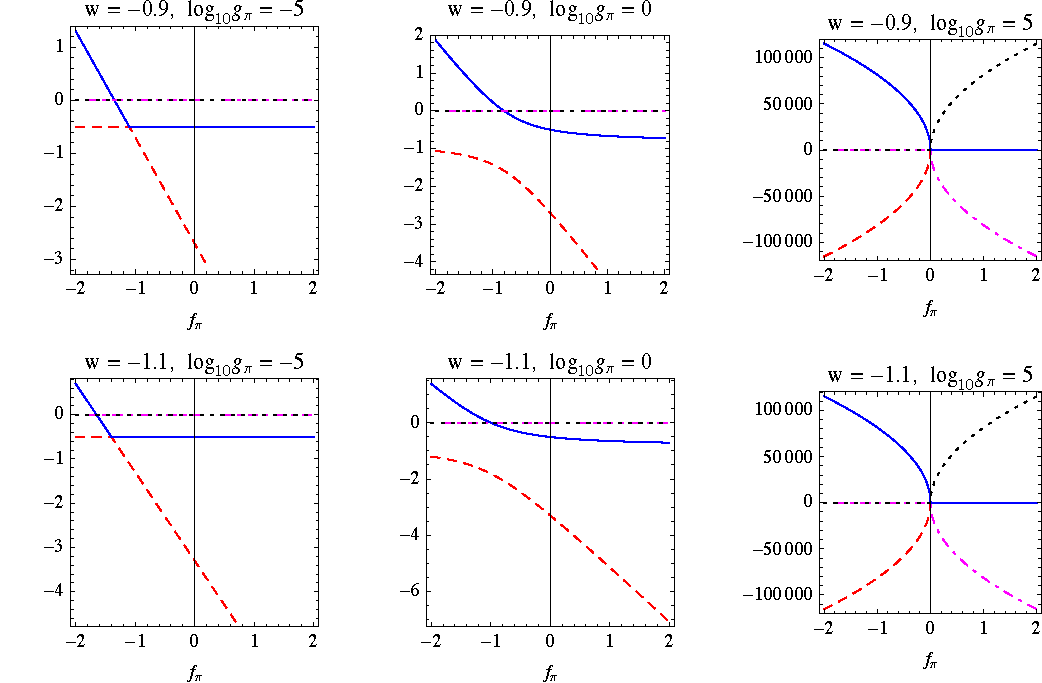
\includegraphics[width=\textwidth]{figures/chapter-ade/expogrid1.pdf}
\caption{The dark energy perturbations during matter domination in the sub-horizon but super-sound horizon regime have a power-law behaviour. Here we show the exponents of the first two terms in Eq. (\ref{eq:pheno9}) for a range of values of the parameters $\ff$ and $\gg$ (the parameter $\aa$ leads to an additional growing mode
driven by the dark matter). Real and imaginary parts for the exponent of the first term are plotted in red dashed and magenta dot-dashed lines, respectively. For the second term the real part is plotted in blue and the imaginary part is shown in black dotted lines. Positive real parts correspond to growing modes, not necessarily instabilities.}
\label{fig:expogrid1}
\end{figure}

%%%%%%%%%%%%%%%%%%%%%%%
\noindent\textbf{Sub-sound horizon}\\
%%%%%%%%%%%%%%%%%%%%%%%

The equations for dark energy velocity and density perturbations in this case are given by
\begin{eqnarray}
V_{de}' &+& \frac{1-6\ceff^2}{2a} V_{de} = -  \frac{\ceff^2 k^2}{H_0^2 \Omega_m}   \delta_{de} \nonumber \\
&+& \frac{\delta_0}{6 H_0^2\Omega_m} \[ 4 \aa a^{n+1} k^2 + 9 H_0^2(1+w)\Omega_m\] \, , \label{eq:pheno11} \\
\delta_{de}' &+& \frac{3(c_s^2-w)}{a}\delta_{de}  = \frac{V_{de}}{a} \, . \label{eq:pheno11b}
\end{eqnarray}
Here we re-introduced the second, sub-dominant term in Eq.\ (\ref{eq:pheno11})  for the special case $\aa=0$.
Like \cite{Sapone:2009kx} we can argue that if we want to avoid large velocity perturbations, then we expect the source terms in Eq.\ (\ref{eq:pheno11}) to cancel to a high degree. It follows that 
\begin{eqnarray} 
\label{eq:pheno12}
\delta_{de} 
&=& a \delta_0 \[ \frac{2 \aa a^n}{3 \ceff^2} + \frac{3 H_0^2 \Omega_m (1+w)}{2 a \ceff^2 k^2} \] \\
V_{de} &=& a \delta_0 \[  \frac{2}{3\ceff^2} \aa a^n \left\{1 + 3 (\ceff^2-w) +2\ff +n \right\} \right. \nonumber \\ 
&&+ \left. \frac{3 H_0^2 \Omega_m \left\{3 (\ceff^2-w) +2\ff \right\}(1+w) }{2 a \ceff^2 k^2 } \] \label{eq:pheno13}
\end{eqnarray}
where the last term in each equation is only relevant if $\aa = 0$. We see that during matter domination
the dark energy perturbations in the sub-sound horizon regime only grow if the coupling to $\Delta_m$ is non-zero.
In that case $\delta_{de}$ is proportional to $a^n \delta_m$. If $e_\pi=0$ then the dark energy perturbations become constant on
sub-sound horizon scales in matter domination. However, it should be mentioned that we have here neglected modes that are 
usually decaying (as in appendix B of \cite{Sapone:2009kx}). As
mentioned at the start of the section, if $\ceff^2<0$ then the full solution of Eq.\ (\ref{eq:pheno7}) grows exponentially.


%%%%%%%%%%%%%%%%%%%%%%%%%%%%%%%%%%%%%%%%%%%
\subsubsection{Dark energy domination and $ \aa = 0 $}\label{subsubsection:3:1:2}
%%%%%%%%%%%%%%%%%%%%%%%%%%%%%%%%%%%%%%%%%%%%

Considering that during dark energy domination the conformal Hubble parameter can be approximated by

\be 
\H^2 = H_0^2 \frac{\Omega_x} {a^{1 + 3 w}}\, ,
\ee 
we find a homogeneous second order equation for the dark energy density perturbations,
\begin{eqnarray}
\label{eq:pheno14}
\delta''_{de} &+&  \bigg\{\,  \frac{3 + 4 \ff - 9 w}{2 a}  \bigg\}\,   \delta'_{de}
+  \bigg\{\, \frac{a^{1 + 3 w} \ceff^2 k^2}{a^2 H_0^2 \Omega_x}  + \frac{\ff ( 2 \gg^2 - 9 - 27 w ) }{3a^2}
 \\ \nonumber
 &-& \frac{3 ( \ceff^2 + \frac{2 \ff}{3} ) \left[6 ( \ceff^2 + \frac{2 \ff}{3})  -  (1 + 4 \ff + 3 w) \right] + 3 (1 - w)(1 + 3 w) }{2 a^2}  \,\bigg\}
 \delta_{de} = 0 \, .
\end{eqnarray} 

Again we can look at both super and sub-sound horizon limits for this equation. \\

%%%%%%%%%%%%%%%%%%%%%
\noindent\textbf{Super-sound horizon}\\
%%%%%%%%%%%%%%%%%%%%%%

In the super-sound horizon limit Eq.\ (\ref{eq:pheno14}) becomes
\be 
\delta''_{de} &+&  \[ \frac{3 + 4 \ff - 9 w}{2 a}  \] \delta'_{de}   \nonumber \\
&+& \[  \frac{4 \ff (-3 + \gg^2 - 9 w) + 9 ( 3 w^2 - 2 w - 1 )  }{6 a^2}  \] \delta_{de} = 0 
\label{eq:pheno15}
\ee

which again has power-law solutions given by 
\be 
\delta_{de} = A_3 a^{\frac{1-\alpha_3 - \beta_3}{2}} + B_3 a^{\frac{1-\alpha_3 + \beta_3}{2}}
\label{eq:pheno16}
\ee
where 
\begin{eqnarray}
\label{eq:pheno17}
\alpha_3 & = & \frac{3+4\ff-9 w}{2} \nonumber \\
\vartheta_3 & = & \frac{4\ff (-3+\gg^2 -9 w) + 9 (3 w^2 - 2 w -1) }{6}\nonumber \\
\beta_3 & = & \sqrt{1-2 \alpha_3 + \alpha_3^2 - 4 \vartheta_3}
\end{eqnarray}
 We plot the behaviour of the exponents in Fig.\ \ref{fig:expogrid3}. Overall, the behaviour is similar to the one shown in Fig.\ \ref{fig:expogrid1}: For small $\gg$ the perturbations can grow rapidly if $\ff \lesssim -3$ while for large $\gg$ they grow quickly whenever $\ff<0$. 
For velocity and matter perturbations we have
\begin{eqnarray} 
\label{eq:pheno16b}
V_{de} &=& \frac{a^{\frac{1-\alpha_3 - \beta_3}{2}}}{2}  \[  B_3 a^{\beta_3} (1+6c_s^2 -6w - \alpha_3 + \beta_3)  + A_3 ( 1+6c_s^2 -6w - \alpha_3 - \beta_3 ) \] \nonumber \\
\delta_m &=& 6(1+2\ff)a^{\frac{1-\alpha_3 - \beta_3}{2}} \[ \frac{B_3 a^{\beta_3}}{(1-\alpha_3 +\beta_3)(2-3w-\alpha_3 + \beta_3)}  \right. \nonumber \\
&& + \left.  \frac{A_3}{(-1+\alpha_3 + \beta_3)(-2+3w+\alpha_3 + \beta_3)}\] + \delta_0  \\
V_m &=& \frac{3(1+2\ff) a^{\frac{1-\alpha_3 - \beta_3}{2}} \[ A_3 (-2+3w+\alpha_3 - \beta_3)  + B_3 a^{\beta_3} (-2+3w+\alpha_3 + \beta_3) \] }{(2-3w-\alpha_3 +\beta_3)(-2+3w+\alpha_3 + \beta_3)} \nonumber
\end{eqnarray}
where we have neglected a decaying mode in the matter density perturbation. We can see that the dark matter density perturbation $\delta_m$ follows the dark energy perturbations and grows at the same rate (in addition to a constant mode). \\

\begin{figure}[tb]
\centering
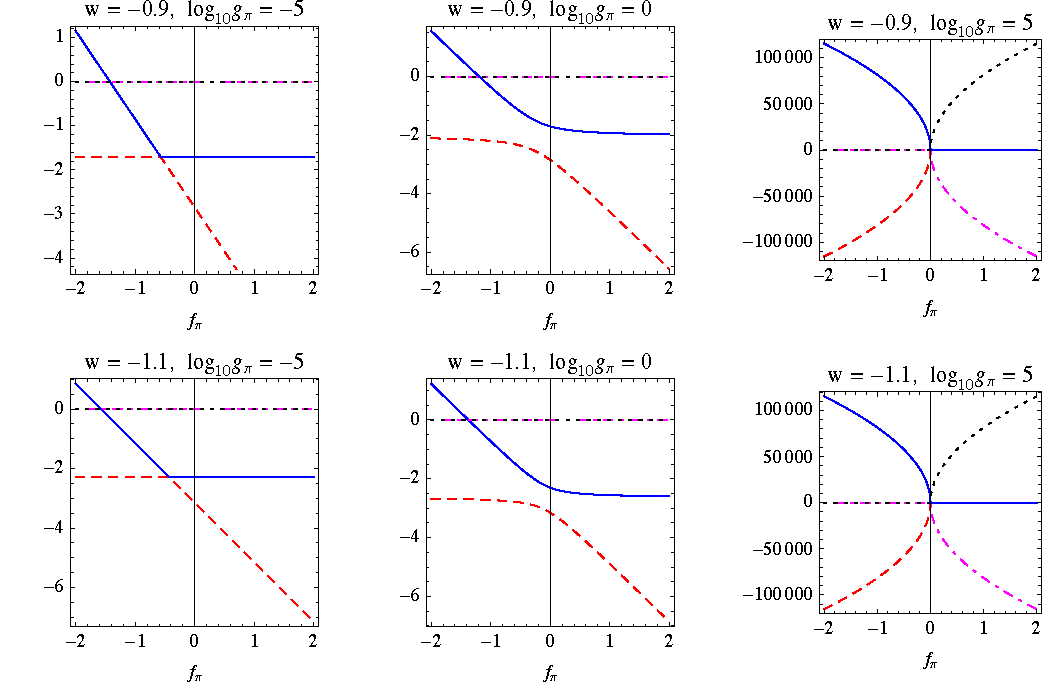
\includegraphics[width=\textwidth]{figures/chapter-ade/expogrid3.pdf}
\caption{The dark energy perturbations during dark energy domination in the sub-horizon but super-sound horizon regime have a power-law behaviour,
with the exponents given here for a range of values of the parameters $\ff$ and $\gg$. Here we plot the exponents of the two terms in Eq. (\ref{eq:pheno16}): red dashed (real part) and magenta dot-dashed (imaginary part) lines correspond to the first term whereas blue (real part) and black dotted (imaginary part) lines correspond to the second term.}
\label{fig:expogrid3}
\end{figure}

%%%%%%%%%%%%%%%%%
\noindent\textbf{Sub-sound horizon}\\
%%%%%%%%%%%%%%%%%%%%


On the other hand, in the sub-sound horizon limit and if we assume 
\be 
\frac{\ceff^2 k^2}{\H^2} \mug \frac{\ff ( 2 \gg^2 - 9 - 27 w ) }{3} - \frac{3 c_{s}^2 \[6 c_{s}^2  -  (1 + 4 \ff + 3 w) \] + 3 (1 - w)(1 + 3 w) }{2}\nonumber
\ee
equation (\ref{eq:pheno14}) reads
\be 
\delta''_{de} &+&  \[ \frac{3 + 4 \ff - 9 w}{2 a}  \] \delta'_{de} +  \[  \frac{\ceff^2 k^2}{ H_0^2 \Omega_x a^{1-3w}}  \] \delta_{de} = 0 
\label{eq:pheno18}
\ee
and we expect to have exponential growth if $ \ceff^2<0 $. The general solution of Eq.\ (\ref{eq:pheno18}) is given by
\begin{eqnarray}
\label{eq:pheno19}
\delta_{de} & = & \(\frac{x_3}{2}\)^{\frac{1-\alpha_4}{1+3w}} \lcb A_4\, J_{\nu_1}(x_3) + B_4\, J_{-\nu_1}(x_3)   \rcb 
\end{eqnarray}
where 
\begin{eqnarray}
\label{eq:pheno20}
\alpha_4 & = & \frac{3+4\ff -9w}{2} \nonumber \\
\nu_1 & = & \frac{\alpha_4 -1}{1+3w} \nonumber \\
x_3 & = & \frac{2 a^{\frac{1+3w}{2}} \ceff k}{(1+3w) H_0\sqrt{\Omega_x}}\, ,
\end{eqnarray}
and $ A_4 $ and $ B_4 $ are constants.\footnote{Gamma functions, similar to those appearing in solutions in Appendix \ref{appendix:2},  have been absorbed in the constants $ A_4 $ and $ B_4 $. These constants are fixed by the initial conditions.} We see that for $\ceff^2<0$ the argument $x_3$ of the Bessel functions becomes imaginary, and indeed the perturbations will grow exponentially. Stable perturbations in this regime thus require $\ff < 3 c_s^2/2$. We can also see that the overall pre-factor of Eq.\ (\ref{eq:pheno19}) behaves like $a^{(1-\alpha_4)/2}$, where the exponent is linearly decreasing with $\ff$, i.e.\ the dark energy perturbations grow faster for more negative $\ff$. We therefore expect also a lower cutoff for $\ff$, around $\ff \approx -7$.

\subsection{Super-horizon scales} 

When considering super-horizon scales, $ k/\H \ll 1 $, we find that dark matter and dark energy perturbations decouple from each other again in matter and dark energy domination. 
However, we could only find analytical solutions during matter dominance.

\subsubsection{Dark matter domination}

Since scales larger than the horizon are also super-sound horizon scales, we can set $ \ceff=0 $ which according to Eq.\ (\ref{eq:pheno2}) is equivalent to setting $ c_s^2 = 2\ff/3 $. Then,  if we use Eq.\ (\ref{eq:pheno4}) for the Hubble parameter and neglect decaying modes, we find the following set of solutions for matter and dark energy perturbations
\begin{eqnarray} 
V_m &=& \delta_0 a \, , 
\qquad 
\delta_m = \delta_0 \frac{3 H_0^2 \Omega_m}{k^2} \, , 
\label{eq:pheno21}
\label{eq:pheno22} \\
V_{de} &=& \delta_0 a \[ \frac{ 4 \aa a^n}{4\ff-3-2n} + \frac{3(1+w)}{ 3-4\ff } \] \,,  
\label{eq:pheno23} \\
\delta_{de}& =&  \delta_0  \frac{3 H_0^2 \Omega_m}{k^2 } \[   \frac{4 \aa a^n (2\ff -3w)}{(4\ff-3-2n)(2\ff +n -3w)} - \frac{3(1+w) }{4\ff -3 }\] \, .
\label{eq:pheno24}
\end{eqnarray} 
We see that outside of the horizon the dark energy density perturbation grows like $a^n$ -- in the particular case when $ n=0 $ or $\aa=0$, the dark energy density perturbation (like the dark matter one) is always constant on super-horizon scales. We also notice that it 
 is non-zero only if either the dark energy is coupled to the dark matter through $\aa\neq0$ or if $w\neq-1$ \footnote{But notice that on sub-horizon scales a non-zero anisotropic stress of the dark energy itself can drive the dark energy perturbations even if $w=-1$ and $\aa=0$, see section \ref{sec:md_subh}. However, for our model 2 the perturbations only grow if $\ff<-5/4$ and only in the sub-horizon but super-sound horizon regime.}.
We also note that we recover the solutions found in \cite{Sapone:2009kx} in the absence of anisotropic stress.


\begin{table}[h!]
\centering
\resizebox{\textwidth}{3.cm}{
\begin{tabular}{|c|c|c|c|}
\hline 
\multicolumn{2}{|c|}{scales} & \multicolumn{2}{|c|}{rapid growth} \\ \cline{3-4}   
\multicolumn{2}{|c|}{} & matter dominance & dark energy dominance ($\aa=0$) \\ \cline{1-4}
\multicolumn{1}{|c|}{\multirow{2}{*}{sub-horizon}} & \multirow{1}{*}{sub-sound}  & $ \phantom{\Bigg|} \ceff^2<0 \phantom{\Bigg|}$  &  $\displaystyle \ceff^2<0 $ \\ \cline{2-4}
 & \multirow{1}{*}{super-sound} & $\phantom{\Bigg|} \ff \ll \dfrac{9w}{2(3+2\gg^2)} \phantom{\Bigg|}$ & $\ff \ll \dfrac{27w^2 -18w -9}{4(3-\gg^2+9w)} $ \\ \cline{1-4}
\end{tabular}}
\caption{Regimes and regions in parameter space where dark energy perturbations grow rapidly.}
\label{tab:stability}
\end{table}

We summarise in Tab.\ \ref{tab:stability} the regions in parameter space where we expect rapid growth of the perturbations
that is not compatible with the existence of a stable universe. The growth of the perturbations on sub-sound horizon scales for $\ceff^2<0$
is exponential and corresponds to the usual instability for negative sound speeds. For theories with a given $c_s^2$ this provides an
upper limit for the parameter $\ff$, namely $\ff < 3 c_s^2 /2$. On scales that are sub-horizon but lie above the sound horizon,
the perturbations grow as a power law with a very high power for sufficiently negative $\ff$, as indicated in the table.\footnote{The regions in the table correspond to the sub and super-sound horizon limits of the second order Eqs. (\ref{eq:pheno7}) and (\ref{eq:pheno14}). Note that according to the general solution for matter dominance and sub-horizon scales, Eq. (\ref{eq:appendix:A1}),  there is also exponential growth on super-sound horizon scales for $ \ceff^2<0 $.} This provides
a lower limit for $\ff$ as such a rapid growth of the dark energy is again not compatible with the data.

In the next section we are going to vary $\ceff>0$ and $\ff$ independently, so that $c_s^2$ can take any value. For this reason we
will not see the upper cutoff on $\ff$ from the instability arising due to $\ceff^2<0$, as we never enter in this regime, but we will
see the lower cutoff. Also, as in the approximate solutions shown in Fig.\ \ref{fig:comparison}, we will limit ourselves to $n=0$ for
the model 1 defined by Eq.\ (\ref{eq:model:1}).

\begin{figure}[tb]
\centering
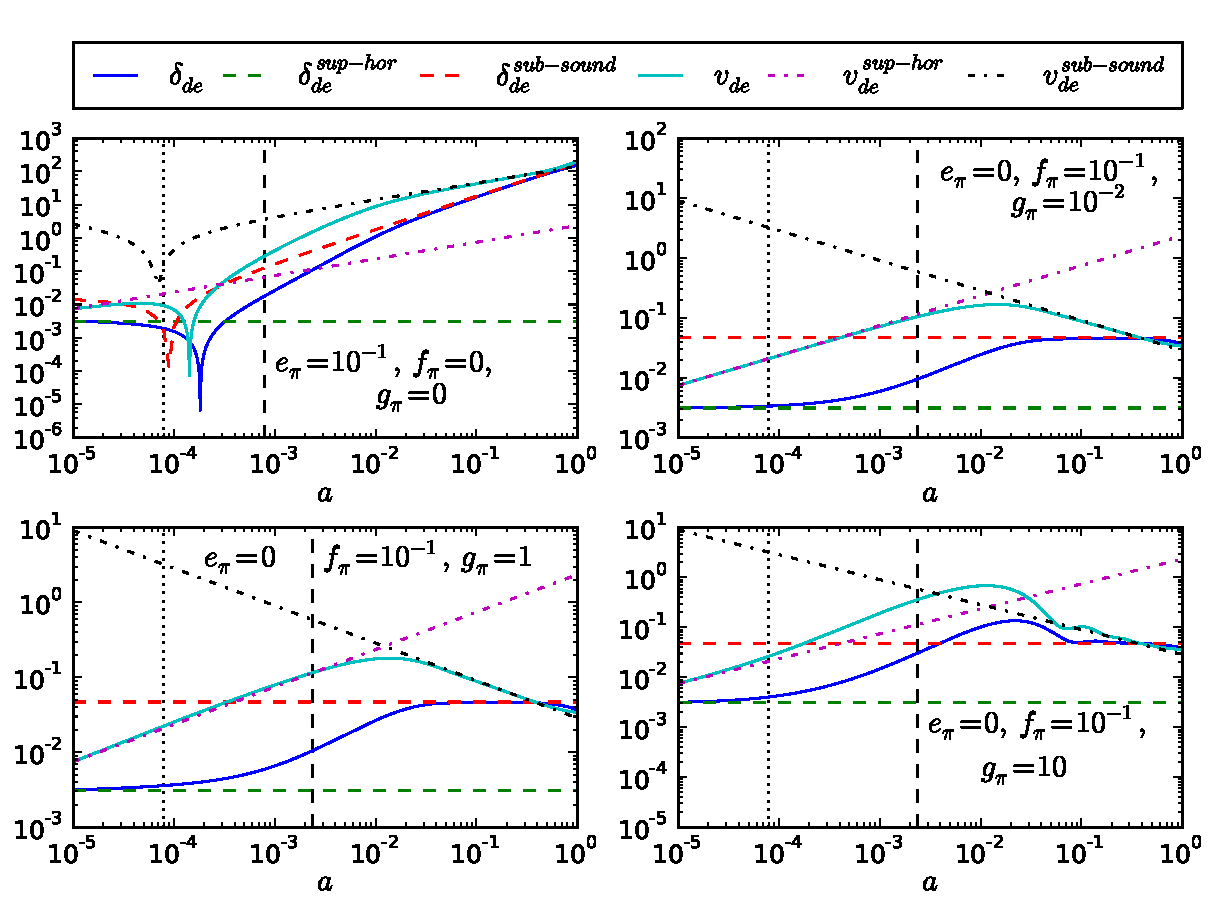
\includegraphics[width=\textwidth]{figures/chapter-ade/comparison.pdf} 
\caption{The figure shows the behaviour of the variables $ \delta_{de} $ and $ v_{de} $ for $k=1.5\times 10^{-2}$, $c_s^2 = 10^{-1}$, $w=-1.05$, $ n=0 $ (the power in Eq. (\ref{eq:model:1})) and different combinations of parameters $\aa$, $\ff$ and $\gg$. The blue and cyan curves are the numerical solutions. Green dashed and magenta dot-dashed curves are analytical solutions on super horizon scales, Eqs. (\ref{eq:pheno23})-(\ref{eq:pheno24}). On the other hand, the red dashed and black dot-dashed curves are analytical solutions on sub-sound horizon scales given by Eqs. (\ref{eq:pheno12})-(\ref{eq:pheno13}). The vertical lines give the scale factor at which the mode enters the effective sound horizon (dashed line) and the Hubble horizon (dotted line). We consider  a longer dynamic range in $a$ to illustrate the transition from super-horizon to sub-sound horizon scales more clearly, without however including radiation in the numerical solution.}
\label{fig:comparison}
\end{figure}

\section{Observational constraints}
\label{chapter-ade:constraints}

In this section, we investigate the parameter degeneracies and the constraints on the anisotropic stress models for dark energy imposed by different cosmological observations. We use a modified version of the {\tt CosmoMC} code (version Mar 13 \cite{Lewis:2002ah,Cosmomc}) to perform Markov-chain Monte-Carlo explorations of the model likelihoods. The sampler calls a modified version of the {\tt CAMB} code\footnote{The modified codes are available at \href{http://cosmology.unige.ch/content/cosmomc-and-camb-early-dark-energy-and-anisotropic-stress}{http://cosmology.unige.ch/content/cosmomc-and-camb-early-dark-energy-and-anisotropic-stress} and the chains (1.4\,GB) can be downloaded from \href{http://theory.physics.unige.ch/~kunz/traces-anisotropic-dark-energy/ade_chains.tar.gz}{http://theory.physics.unige.ch/$ \sim $kunz/traces-anisotropic-dark-energy/ade$\_$chains.tar.gz}.} (version Mar 13 \cite{Lewis:1999bs,Camb}) to compute the linear theory CMB spectra for a given model. 
In all cases we use constraints on the number of relativistic degrees of freedom at Big-Bang nucleosynthesis (BBN) \cite{Pisanti:2007hk} and put a prior on the age of the Universe to be between 10 and 20 Gyrs. In addition we use the CMB likelihood code of the Planck collaboration (version 1.0 \cite{Planck:2013kta,Ade:2013zuv}) which includes the Planck first data release combined with WMAP 9yr low-multipole polarisation data \cite{Bennett:2012fp}. Moreover, we add the high-multipole temperature data from the South Pole Telescope (SPT) \cite{Story:2012wx} and the Atacama Cosmology Telescope (ACT) \cite{Das:2013zf}. In the following, we use the abbreviation \emph{CMB data} for the combination of Planck temperature, WMAP9 low-multipole polarisation, and ACT and SPT temperature  (referred to as \emph{Planck}+WP+highL in the Planck papers). We expect the CMB data to provide constraints not only on the parameters that describe the primordial power spectrum and the re-ionisation history but also to mildly constrain the late-time evolution of the gravitational potentials through the integrate Sachs-Wolfe effect and CMB lensing. 


To further constrain the parameters that are relevant for the late-time evolution of the background geometry, the density parameter and equation of state of dark energy, we also use constraints on the distance--redshift relation from baryon acoustic oscillations (BAO) and type Ia supernovae (SNe). Currently, there are seven BAO measurements available: two from the Sloan Digital Sky Survey (SDSS) DR7 
\cite{Percival:2009xn,Padmanabhan:2012hf}, one from the 6dF Galaxy Survey 
\cite{Beutler:2011hx}, three from the WiggleZ Dark Energy Survey 
\cite{Blake:2011en}, and one from the SDSS-III Baryon Oscillation Spectroscopic Survey (BOSS) DR9 
\cite{Anderson:2012sa}. In case of the supernovae, we use the compilation of 473 SNe Ia provided by the SuperNova Legacy Survey (SNLS) team \cite{Conley:2011ku}.
The fact that Planck prefers a slightly different value for $H_0$ than local measurements of the Hubble parameter in a flat $\Lambda$CDM cosmology raises concerns about the compatibility of these data sets \cite{Ade:2013zuv}. For this reason we chose not to include constraints on the local expansion rate. If we included
the $H_0$ constraint of \cite{Riess:2011yx} we would find that the confidence intervals for $w$ are shifted slightly towards more
negative values, with $w = -1$ sitting close to the $2 \sigma$
limit. On the other hand, we would not find significant changes in the
constraints on the parameters that govern the dark energy
perturbations when including $H_0$ data.

Using large-scale structure data like the galaxy power spectrum $P(k)$ correctly in the context
of dark energy and modified gravity models is quite involved. There are hidden model assumptions
in the analysis of the data and the construction of the likelihood. For example, the background cosmology
is used when
converting angles and redshifts to $k$ vectors. Moreover, the impact of modifications of  
gravity on galaxy bias and non-linear clustering is mostly unknown. For these reasons we limit ourselves for the time
being to the data sets mentioned above.

For the parameter estimation we vary a base set of seven parameters (those of the flat wCDM model). These are the amplitude, $\ln[10^{10}A_s]$, and the tilt, $n_s$, of the spectrum of primordial scalar curvature perturbations (modelled as a power law normalised at $k=0.05\,{\rm Mpc}^{-1}$), the reionisation optical depth, $\tau$, the physical baryon and cold dark matter energy fractions, $\Omega_b h^2$ and $\Omega_c h^2$, 100 times the ratio of the sound horizon to the angular diameter distance to the last-scattering surface, $\theta$, and finally the constant equation of state parameter of dark energy, $w$. In the figures we will replace the ``fundamental'' parameters $A_s$ and $\theta$ by the variance of fluctuations in spheres of 8 Mpc today, $\sigma_8$, and the value of the Hubble parameter today, $H_0$ (in units of km$/$s/Mpc), that are both derived parameters.

In addition to the base model, we vary or fix the values of the parameters that describe the properties of the dark energy perturbations: the effective sound speed, $\log_{10}\ceff^2$, the external anisotropic stress parameter, $e_\pi$, and the internal anisotropic stress parameter, $f_\pi$, with its transition scale, $\log_{10}g_\pi$. We use flat priors for all parameters, set adiabatic initial conditions for the evolution of the cosmological perturbations, and ignore vector and tensor modes for simplicity.

\begin{figure}[tb]
\centering
\begin{lpic}[clean]{figures/chapter-ade/PWHiBSwefc_tri(14.cm,)}
\lbl[l]{90,185; \footnotesize\textcolor{blue}{\bf ---}\quad CMB =
Planck + WP + highL}
\lbl[l]{90,175; \footnotesize\textcolor{red}{\bf ---}\quad CMB + BAO}
\lbl[l]{90,165; \footnotesize\textcolor{black}{\bf ---}\quad CMB + BAO + SNe}
\end{lpic}\\[-0.8cm]
\caption{Marginalised 2d likelihoods and 1- and 2-$\sigma$ contours of combinations of the model parameters $\{w$, $e_\pi$, $f_\pi$, $\log_{10}g_\pi$, $\log_{10}\ceff^2\}$. We compare the use of different data sets: blue is \emph{CMB data} only, red is \emph{CMB+BAO}, and black and the likelihood density plots are \emph{CMB+BAO+SNe}. In all cases we vary all parameters.}
\label{fig:2d_data}
\end{figure}

Let us first take a look at the effect of the different data sets on the parameter constraints. In figure \ref{fig:2d_data} we show the marginalised posteriors and the marginalised 2d-likelihood contours of a parameter subset in the full model, i.e.\ varying all dark energy parameters including the anisotropic stress model, $e_\pi$, $f_\pi$, $g_\pi$ (for $n=0$). We compare the effect of adding more data: blue is \emph{CMB data} only, red is \emph{CMB+BAO}, and black and the likelihood density plots are \emph{CMB+BAO+SNe}. For parameters that are not related to dark energy anisotropic stress the likelihood contours shrink considerably when adding the low-redshift data, as they contain much information on the late-time expansion and therefore on $w$. The constraints on the anisotropic stress parameters are not much altered by adding low-redshift data because BAO and SNe do not contain information on the growth of structure that is affected by the dark energy clustering. To improve those constraints we would need to add information on galaxy clustering, redshift space distortions and cosmic shear.

 The $(\ff,\, \log_{10}g_\pi)$ plane also shows nicely the lower limit on $\ff$ from the rapid growth of perturbations. As argued in the discussions of the sub horizon / super-sound horizon perturbation evolution in  section \ref{subsection:4.1} and shown in  Figs.\ \ref{fig:expogrid1} and \ref{fig:expogrid3}, a very negative value of $\ff$ is in conflict with observations as the dark energy perturbations become large. We can also see how the lower limit on $\ff$ changes as a function of $\gg$, with $\gg \mug 1$ requiring $\ff>0$. 
 
It is interesting to note that the marginalised likelihood in the $(\log_{10}\ceff^2,\, \ff)$ plane peaks where $f_\pi$ is negative and $\log_{10}\ceff^2$ close to 0, while the $(\ff,\, \log_{10}g_\pi)$ plane shows that the likelihood for negative $f_\pi$ is much lower than for positive $\ff$. Note that this is a volume effect of the marginalization. If we were to fix $\ceff=1$, then the high plateau of the likelihood in the $(\ff,\, \log_{10}g_\pi)$ plane would shift from the positive--positive to the negative--negative quadrant, and the situation would be quite different.

Thus, if we had additional observables that even more strongly prefer $\ceff=1$, we would conclude $f_\pi \leq 0$. The constraints on $e_\pi$ would not be affected as it is virtually not degenerate with $\log_{10}\ceff^2$. There is a hint that this could actually be the case: the CFHTLens weak lensing survey \cite{Kilbinger:2012qz} as well as the Planck cluster counts \cite{Ade:2013lmv} prefer $\sigma_8$ and $\Omega_m$ considerably lower than Planck alone (in the $\Lambda$CDM model). We added a toy constraint on the combination $\sigma_8(\Omega_m/0.27)^{0.6}$ that reflects the weak lensing and cluster counts, and noticed that it is passed through the parameter degeneracies in such a way that it constrains $\ceff^2 \sim 1$ and $f_\pi$ and $\log_{10}g_\pi$ both negative. In this case $f_\pi$ turns out to be strongly constrained and $f_\pi=0$ is already in quite some tension with the toy data. We interpret this as a hint that additional dark energy degrees of freedom are able to reconcile apparent tensions between different current data sets. However, we emphasise that the analysis of the weak lensing and cluster count likelihood needs to be done fully correctly within the framework of a generalised dark energy model like ours, and the constraints quoted in the literature \cite{Kilbinger:2012qz, Ade:2013lmv} cannot directly be implemented since they are derived for the $\Lambda$CDM model.


\begin{figure}[tb]
\centering
\begin{lpic}[clean]{figures/chapter-ade/PWHiBSwefc_models_tri(14.cm,)}
\lbl[l]{90,186; \footnotesize\textcolor{green}{\bf ---}\quad
$(\aa,f_\pi,\,\log_{10}g_\pi)=(0,0,0)\,$, varying
$(w,\,\log_{10}\ceff^2)$ }
\lbl[l]{90,177; \footnotesize\textcolor{blue}{\bf ---}\quad
$(f_\pi,\,\log_{10}g_\pi,\,\log_{10}\ceff^2)=(0,0,0)\,$, varying
$(w,\,e_\pi)$}
\lbl[l]{90,168; \footnotesize\textcolor{red}{\bf ---}\quad
$(f_\pi,\,\log_{10}g_\pi)=(0,0)\,$, varying
$(w,\,e_\pi,\,\log_{10}\ceff^2)$}
\lbl[l]{90,159; \footnotesize\textcolor{black}{\bf ---}\quad varying
$(w,\,f_\pi,\,\log_{10}g_\pi,\,\log_{10}\ceff^2)$}
\end{lpic} \\[-0.8cm]
\caption{Marginalised 2d likelihoods and 1- and 2-$\sigma$ contours of combinations of the model parameters $\{n_s$, $\sigma_8$, $w$, $e_\pi$, $f_\pi$, $\log_{10}g_\pi$, $\log_{10}\ceff^2\}$. We compare the different models: 
 for blue we fix $(f_\pi,\,\log_{10}g_\pi,\,\log_{10}\ceff^2)=(0,0,0)$, for red we fix $(f_\pi,\,\log_{10}g_\pi)=(0,0)$, and for black and the likelihood density plots we vary all parameters (except for the scaling exponent $n$ of model 1 which is always set to $n=0$). Here we are using the full data set,  \emph{CMB+BAO+SNe}.}
\label{fig:2d_models}
\end{figure}

Next, let us study the anisotropic stress model parameters. In figure \ref{fig:2d_models} we show the marginalised posteriors and 2d-likelihoods using the full data set, \emph{CMB+BAO+SNe}. We compare the different models: for green we fix $(e_\pi,\,f_\pi,\,\log_{10}g_\pi)=(0,0,0)$, for blue we fix $(f_\pi,\,\log_{10}g_\pi,\,\log_{10}\ceff^2)=(0,0,0)$, for red we fix $(f_\pi,\,\log_{10}g_\pi)=(0,0)$, and for black and the likelihood density plots we vary all parameters. We observe that in case of no anisotropic stress, green, the dark energy sound speed is only very mildly preferred to be close to 1, as expected from earlier studies, see e.g.\ \cite{Bean:2003fb,dePutter:2010vy}. Finally, in figure \ref{fig:1d_other} we show the marginalised posteriors for the remaining six base parameters, $\{\Omega_bh^2$, $\Omega_ch^2$, $n_s$, $\tau$, $\sigma_8$, $H_0\}$, that are not directly related to dark energy. We note that all models with dark energy anisotropic stress slightly prefer a higher $\sigma_8$ than in the smooth dark energy case, $\ceff=c_s=1$ (see \cite{Kunz:2003iz} for a study of the impact of $w$ on $\sigma_8$ in smooth dark energy models). This is compatible with the discussion above on the slight tension between constraints on $\sigma_8$ from Planck CMB and Planck cluster counts as well as weak lensing.


\begin{figure}[tb]
\centering
\vspace{2 cm}
\begin{lpic}[clean,nofigure]{figures/chapter-ade/fig-6-nolabel(14.cm,)}
\lbl[l]{10,175; \footnotesize\textcolor{black}{\bf ---}\quad
CMB$ + $BAO$ + $SNe}
\lbl[l]{10,166; \footnotesize\textcolor{red}{\bf ---}\quad
CMB$ + $BAO}
\lbl[l]{10,157; \footnotesize\textcolor{blue}{\bf ---}\quad
CMB$ = $PLANCK$ + $WP$ + $highL}
\lbl[l]{130,180; \footnotesize\textcolor{black}{\bf ---}\quad varying
$\log_{10} \ceff^2,\, \aa,\,f_\pi,\,\log_{10}g_\pi$}
\lbl[l]{130,171; \footnotesize\textcolor{red}{\bf ---}\quad varying
$ \log_{10}\ceff^2,\,\aa $}
\lbl[l]{130,162; \footnotesize\textcolor{blue}{\bf ---}\quad varying
$ \aa $}
\lbl[l]{130,153; \footnotesize\textcolor{green}{\bf ---}\quad varying
$ \log_{10}\ceff^2 $}
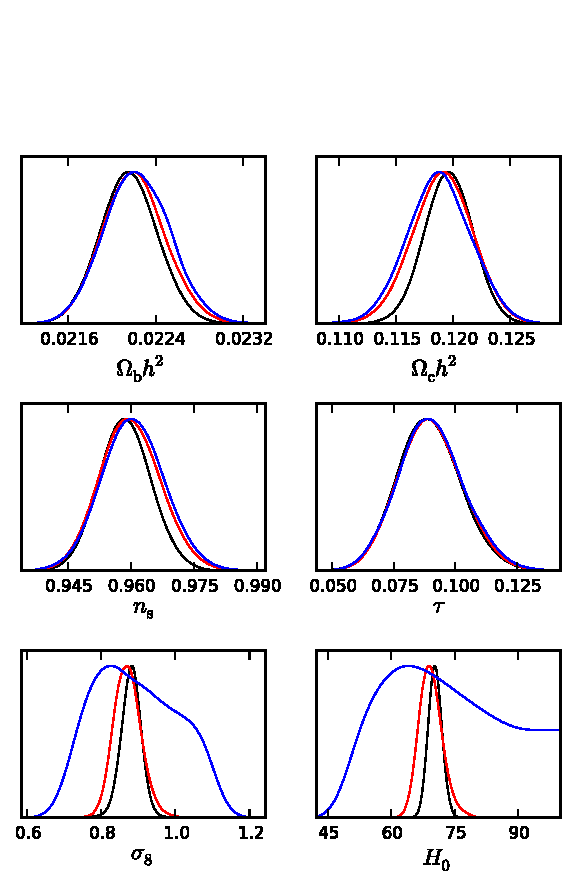
\includegraphics[width=.48\textwidth]{figures/chapter-ade/PWHiBSwefc_nolabel2}\ 
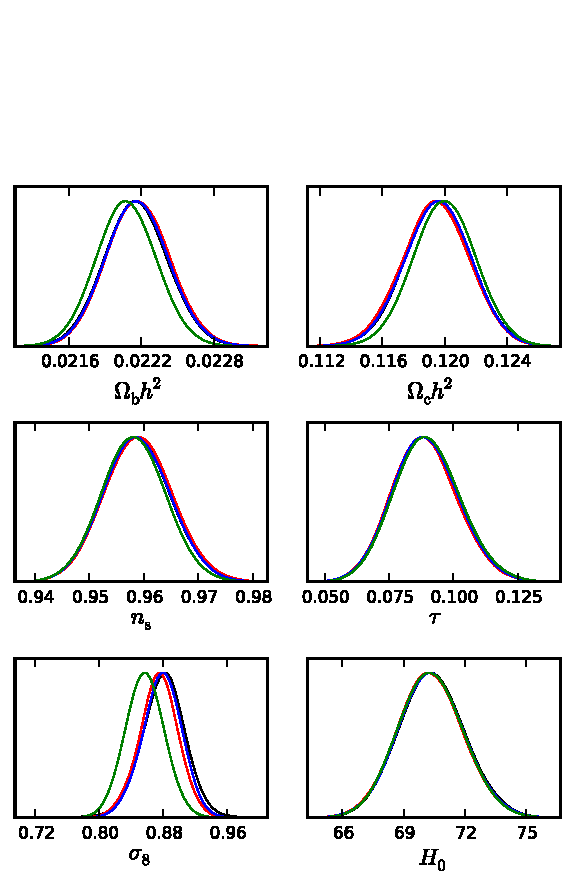
\includegraphics[width=.50\textwidth]{figures/chapter-ade/PWHiBSwefc_models_nolabel}
\end{lpic}\\[-0.1 cm]
\caption{Marginalised posteriors of those model parameters not directly related to dark energy $\{\Omega_bh^2$, $\Omega_ch^2$, $n_s$, $\tau$, $\sigma_8$, $H_0\}$. 
\emph{Left panel}: comparison of different data sets as in figure \ref{fig:2d_data}. The addition of background data sets helps to constrain especially $H_0$ and $\sigma_8$.
\emph{Right panel}: comparison of different models as in figure \ref{fig:2d_models}. The constraints on these parameters do not change significantly when the anisotropic stress is non-zero, with the exception of $\sigma_8$ which prefers a slightly higher value.}
\label{fig:1d_other}
\end{figure}

\begin{figure}[tb]
\centering
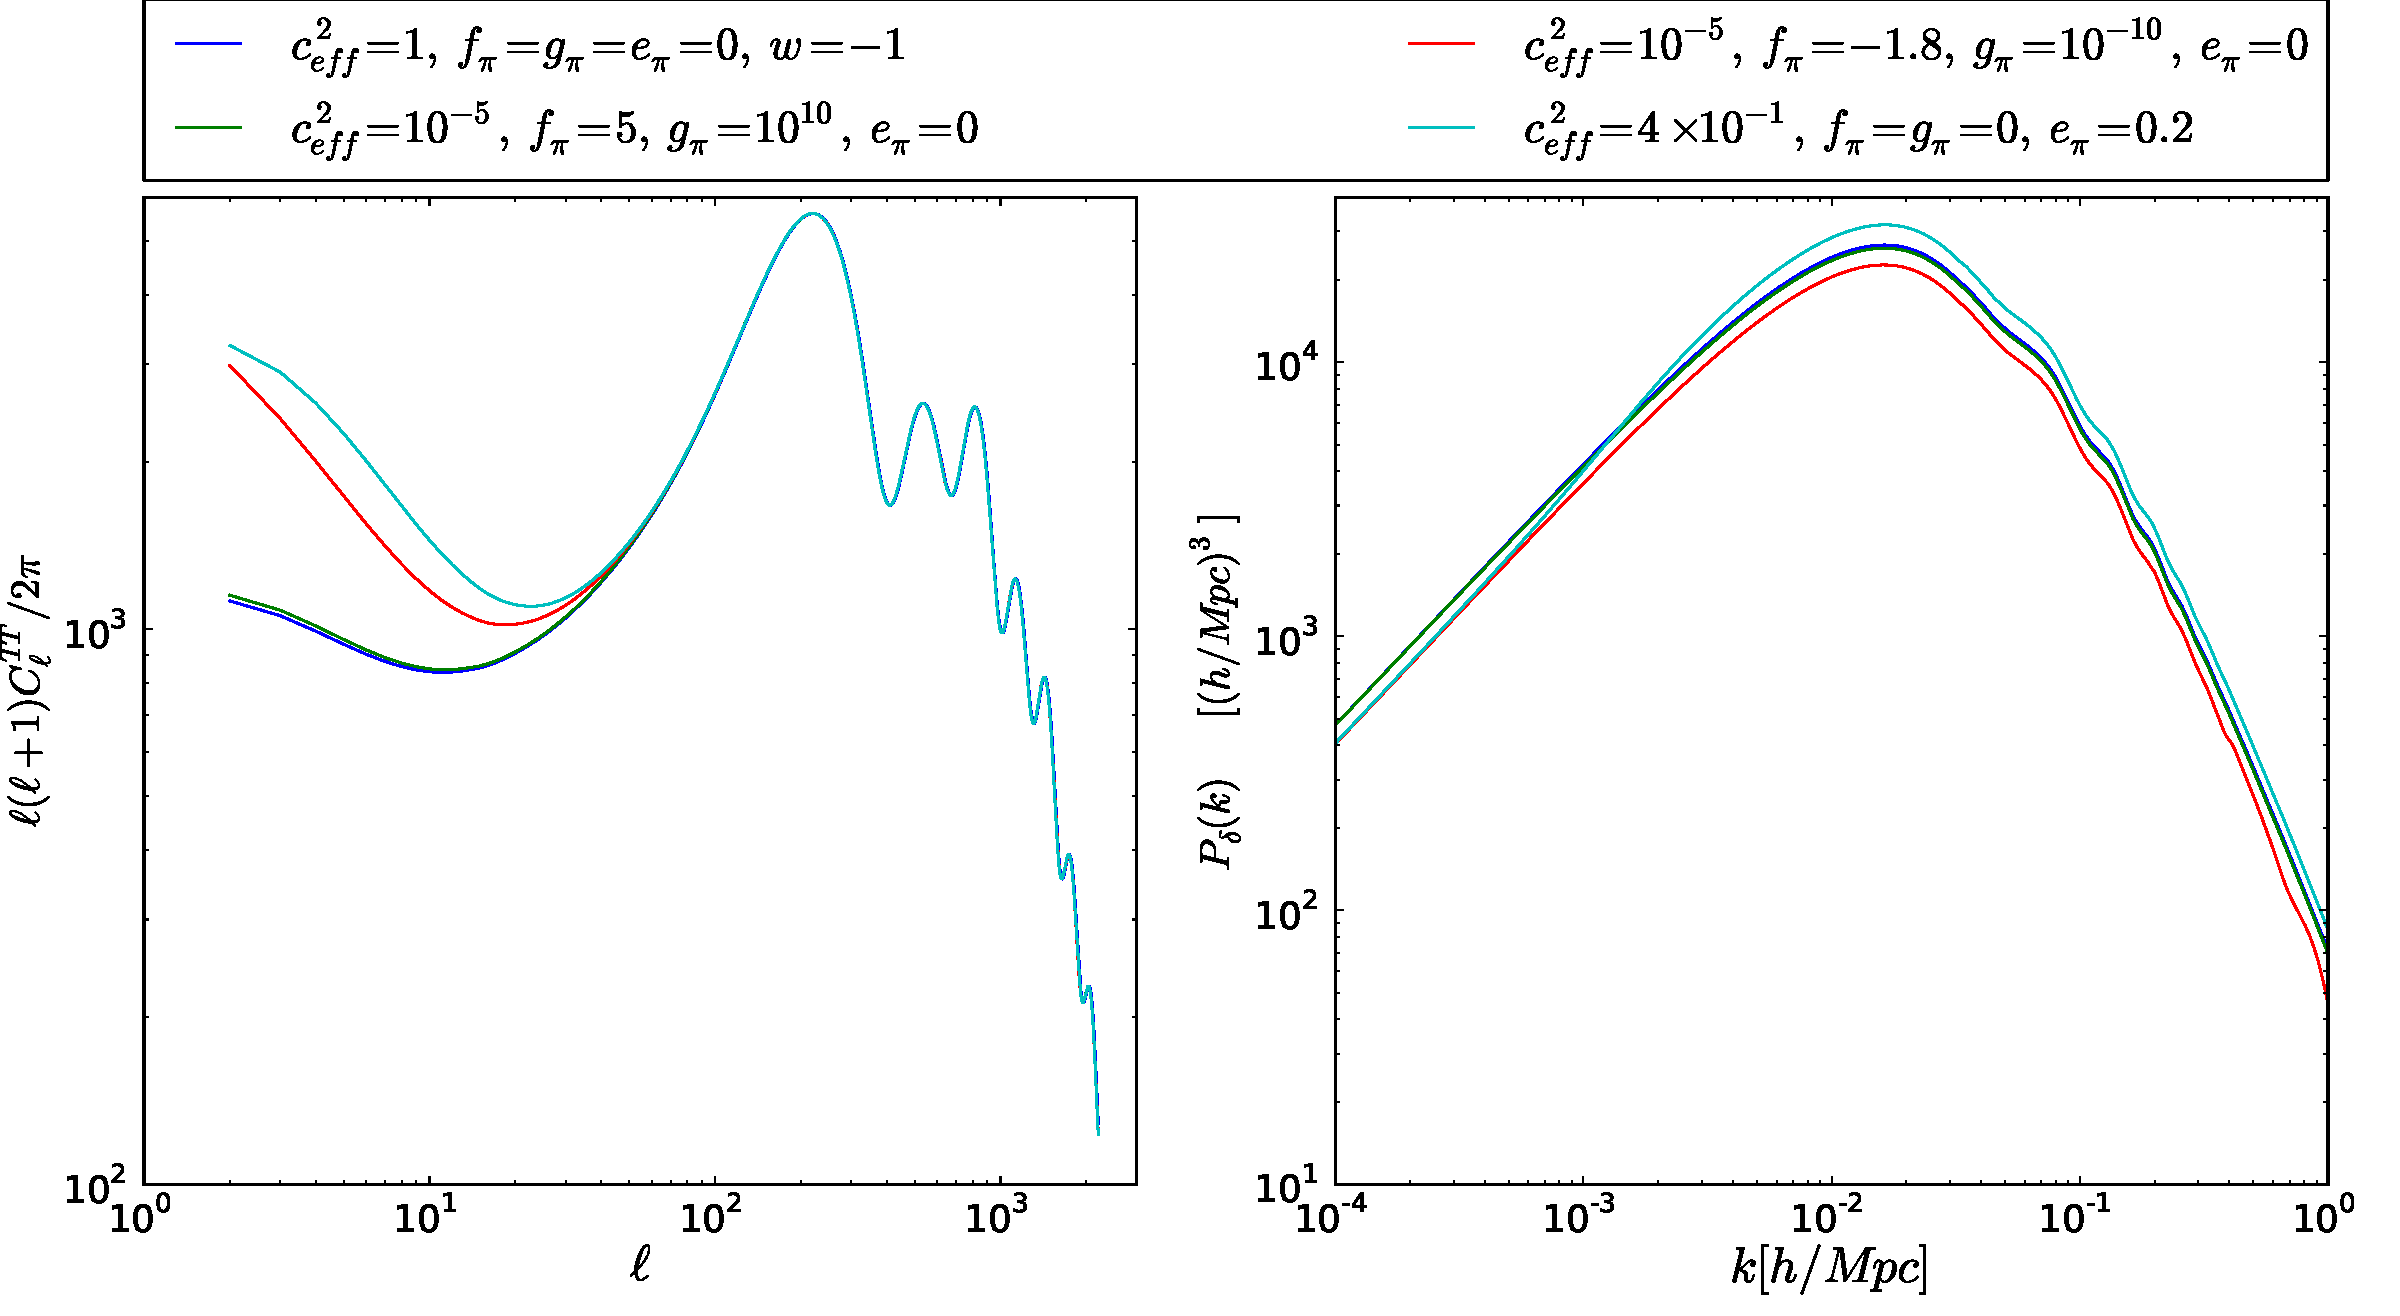
\includegraphics[width=\textwidth]{figures/chapter-ade/PkCls_2}
\caption{CMB angular power spectra (left panel) and matter power spectra (right panel). The concordance model is shown in blue. In green we plot a model with internally sourced anisotropic stress whose parameters are allowed by the cosmological constraints. Two models with parameters excluded by cosmological constraints are depicted in red (internally sourced anisotropic stress) and cyan (externally sourced anisotropic stress). For those models different from the concordance model we used $ w=-0.95 $. In the CMB the differences appear on large scales as the ISW effect is strongly affected by the late-time anisotropic stress of the dark energy. The impact on the matter $P(k)$ is less strong and on scales smaller than the peak appears mostly as a shift in the normalisation (and thus a shift in $\sigma_8$), although this is different on large scales (that are however difficult to observe in galaxy surveys). The effect looks degenerate with an early dark energy contribution (see e.g.\ Fig.\ 5 of \cite{Hollenstein:2009ph}) and it may also be difficult to distinguish observationally from galaxy bias.}
\label{fig:pk-cls}
\end{figure}


\section{Modified growth parametrisations}
\label{chapter-ade:growth}

In this paper we used prescriptions for the ``hydrodynamical'' closure relations that define $\delta P$ and $\pi$ in terms of
other variables, in order to complete the system of equations. Instead of defining the dark energy momentum tensor, it is also
possible to introduce functions that describe the change to the matter growth rate \cite{Amendola:2004wa,Linder:2005in} or that modify the
Einstein equations with an effective Newton's constant and a gravitational slip \cite{Amendola:2007rr}. The latter
parametrisation is in principle equivalent to giving $\delta P$ and $\pi$ as shown explicitly
in \cite{Ballesteros:2011cm}, but the modified growth rate on its own is not sufficient and needs to be supplemented 
by an additional condition. We will call these approaches `modified growth' parameterisations, see also section 1.3.2
of \cite{Amendola:2012ys} for a more detailed introduction.

As the modified growth approach is quite popular and since several groups have derived predictions for the accuracy
with which these parameters can be measured (e.g.\ \cite{Amendola:2007rr,Pogosian:2010tj,Bean:2010zq}), we give here the expressions necessary to compute these
quantities in general and discuss the links between them and our parametrisation. We then show what bounds we
can infer on these modified growth parameters from the data that we use, in the context of our model.

%%%%%%%%%%%%%%%%%%%%%%%%%%%%%%%%%%%%%%%%%%%%%%%%%%%%%%%%%%%%%%%%%%%%%%%%%%%%%%%%%
\subsection{Definition of the modified growth parameters}

In general the presence of a dark energy fluid or of a modification of General Relativity will affect the growth rate of the
dark matter perturbations.
We define the growth factor $g$ as the logarithmic derivative of the comoving matter density perturbation,
\be
  g\ \equiv\ \frac{d\log \Delta_m}{d\log a}
\ee
The growth factor is often approximated using the growth index, $\gamma$, as
\be
  g\ =\ \Omega_m(a)^\gamma
\ee
where $\Omega_m(a)\equiv 8\pi Ga^2\rho_m(a)/(3\H^2)$. In general, $g$ and $\gamma$ are space and time dependent functions. To investigate $\gamma$ we express it in terms of $g$
\be
  \gamma\ =\ \frac{\log g}{\log \Omega_m(a)}
\ee
and we have implemented these expressions in CAMB so that we can obtain limits on $g$ and $\gamma$
as derived parameters from our MCMC chains.

However, in general we have two scalar degrees of freedom, related to the possibility to choose independent closure relations for
both $\delta P_{de}$ and $\pi_{de}$ in the fluid picture. To model these two degrees of freedom, 
we introduce a parameter $Q$ which describes either an effective Newton's constant $Q G$ or an additional contribution
to the clustering from $\Delta_{de}$ through the Poisson equation for $\phi$.
In addition, we parameterise the gravitational slip (the difference of the gravitational potentials which is in our model due to the
anisotropic stress of the dark energy) as $\eta$,
\be
Q \equiv \frac{- k^2\phi}{4\pi G a^2 \rho_m \Delta_m}
= 1+ \frac{\rho_{de} \Delta_{de}}{\rho_m \Delta_m}
\,, \qquad
\eta \equiv \frac{\phi}{\psi} \, .
\ee
$\eta$ should not be confused with conformal time, obviously. This parameter is occasionally called $\varpi$ in the literature.

We can now derive some relations between different parameters. For example we have that
\be
\frac{1}{\eta} = 1+ \frac{2}{Q} \frac{\rho_{de} \pi_{de}}{\rho_m \Delta_m} = 1+ \frac{2 \rho_{de} \pi_{de}}{\rho_m \Delta_m + \rho_{de} \Delta_{de}} \, .
\ee
In a pure model 1 situation, i.e.\ with $f_\pi=0$, we then have that
\be
\frac{1}{\eta} = 1+ \frac{2 e_\pi}{Q} \frac{\rho_{de} }{\rho_m } = 1+ \frac{2 e_\pi}{Q} \frac{\Omega_{de}}{\Omega_m} a^{-3 w} \approx 1+ \frac{2 e_\pi}{Q} \, ,
\label{eq:q_eta}
\ee
where the final expression is valid at late times for our averaging (see below). 

%%%%%%%%%%%%%%%%%%%%%%%%%%%%%%%%%%%%%%%%%%%%%%%%%%%%%%%%%%%%%%%%%%%%%%%%%%%%%%%%%
\subsection{Constraints on the modified growth parameters in our model}

In general the modified growth parameters are functions of scale and time. We limit here our investigation to the late-time behaviour,
by averaging the parameters over the range $z=0\ldots 1$ using 10 values linearly spaced in $z$. The scale dependence can be
important, so we consider separately `large' scales, $k = 10^{-3} \,h\, \Mpc^{-1}$ and `small' scales, $k = 10^{-1} \,h\, \Mpc^{-1}$. 

In Fig.\ \ref{fig:3d} we show $Q$ and $\eta$ values of a sample of `type 1' models accepted by the MCMC algorithm where $\aa$ varies and $\ff$ is zero. In the first column
we also fix $c_s=1$ (which is equivalent to $\ceff=1$ as $\ff=0$), and in this case we can access only a narrow region in $(Q,\eta)$
space. This is not unexpected as in general we need to vary both $\delta P_{de}$ and $\pi_{de}$. When doing so in the second and third column,
and now a much larger part of the $(Q,\eta)$ parameter space is accessible.  This also illustrates that our models are able to probe
quite generally the space of modifications of the growth parameters.

We can also see very nicely from the colours in the first two columns of Fig.\ \ref{fig:3d} how a non-zero $\aa$ changes the growth
rate $\gamma$, with pretty much a one-to-one mapping between the two on small scales. The sound speed on the other hand leads to a rotation
in the $(Q,\eta)$ parameter space on small scales.

\begin{figure}[tb]
\centering
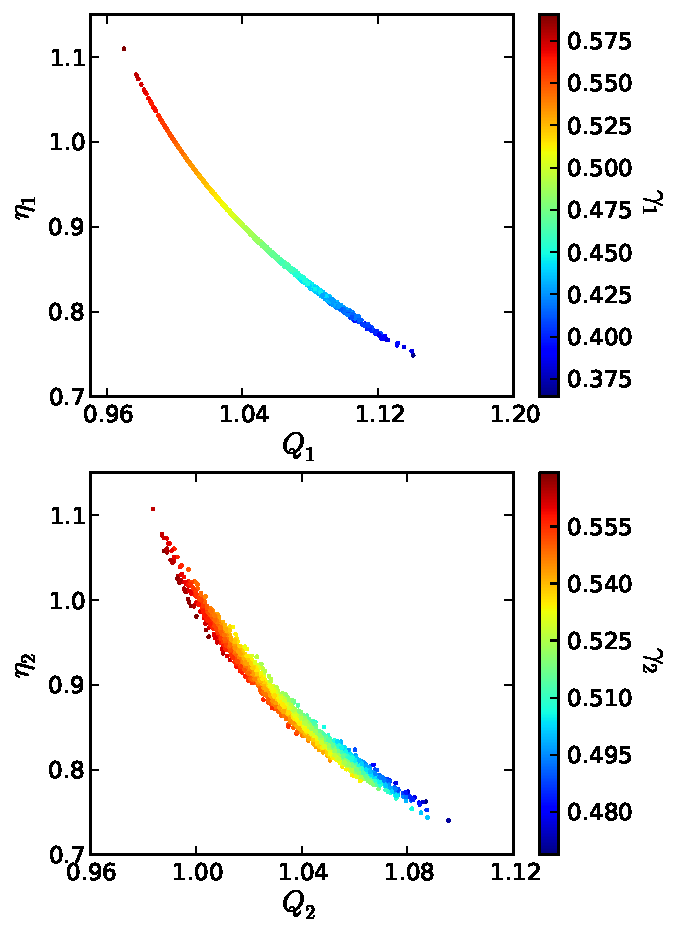
\includegraphics[width=0.32\textwidth]{figures/chapter-ade/PWHiBSwe0_3D_gamma.pdf}
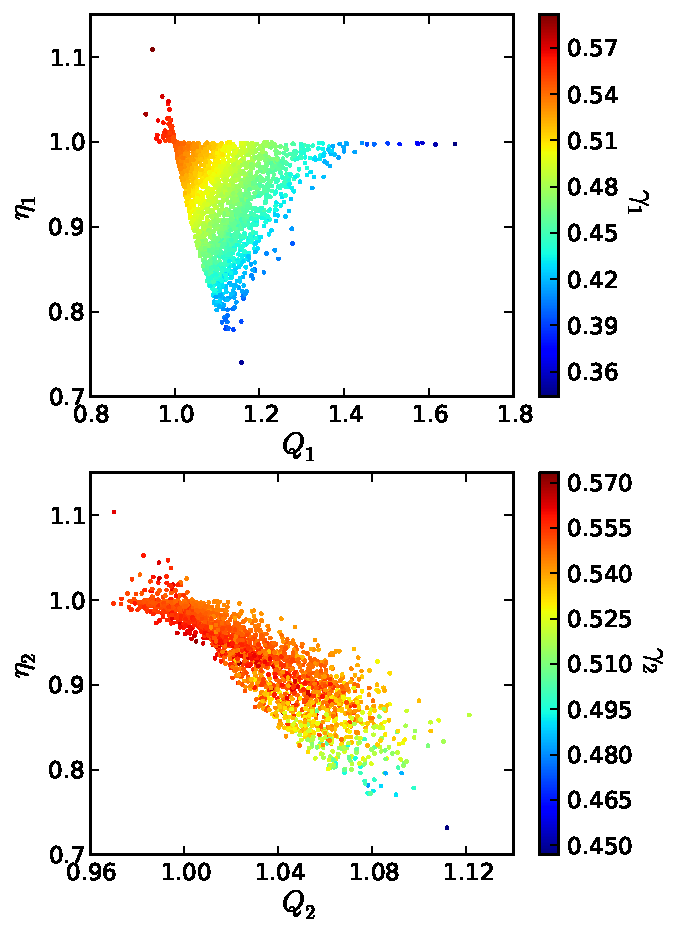
\includegraphics[width=0.32\textwidth]{figures/chapter-ade/PWHiBSwec_3D_gamma.pdf}
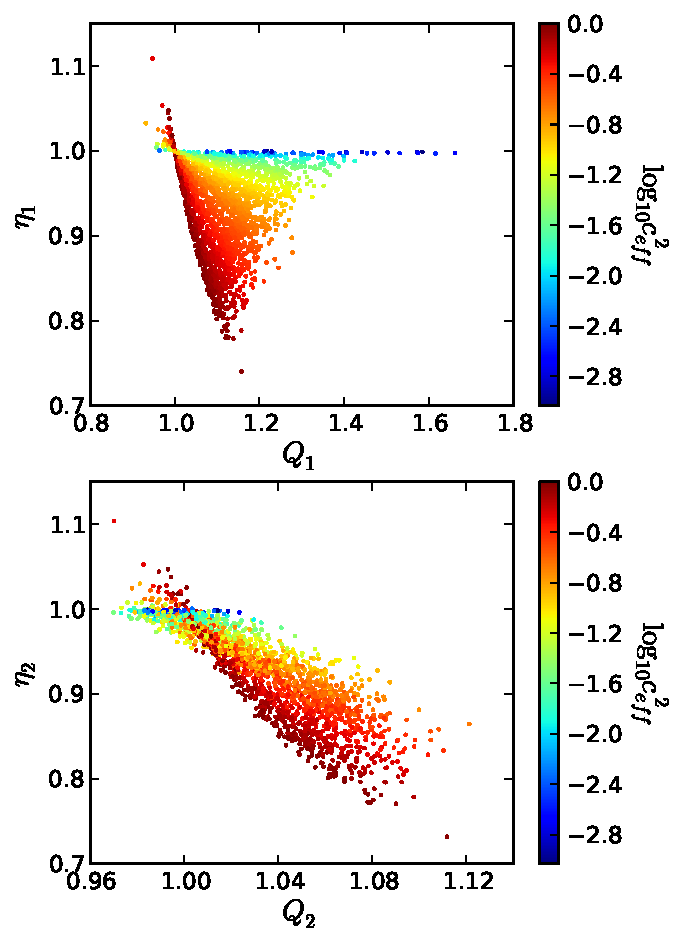
\includegraphics[width=0.32\textwidth]{figures/chapter-ade/PWHiBSwec_3D_ceff.pdf}
\caption{Scatter plots of samples of accepted models in our MCMC chains for $\ff=0$ and $\aa$ varying,  when using the full data set, \emph{CMB+BAO+SNe}. The lower row of figures shows the behaviour on large scales $( k_1 = 10^{-3} \,h\,\Mpc^{-1})$, while the upper row depicts smaller scales $ (k_2 = 10^{-1} \,h\,\Mpc^{-1}) $.  \emph{First column:} the sound speed is held fixed, $c_s=1$, and the growth index, $\gamma$, nicely parametrises the single allowed line in the $(Q,\,\eta)$ plane. \emph{Second column:} the sound speed is allowed to vary, a whole area is sampled in the $(Q,\,\eta)$ plane, and the growth index only parametrises one direction. \emph{Third column:} the other direction is parametrised by the sound speed.}
\label{fig:3d}
\end{figure}

We can understand this latter behaviour with the help of the relation (\ref{eq:q_eta}): The presence of an anisotropic stress induced
by $\aa$ impacts not only $\eta$, but also $Q$. On sub-sound-horizon scales and during matter domination the induced dark energy
perturbations are given by Eq.\ (\ref{eq:pheno12}),
\be
\Delta_{de} \approx \delta_{de} \approx a \delta_0  \left( \frac{2 e_\pi a^n}{3 \ceff^2} \right) \approx \left( \frac{2 e_\pi a^n}{3 \ceff^2} \right) \Delta_m \, ,
\ee
and therefore we have in that limit that
\be
Q = 1 + \frac{2 \aa a^n}{3 \ceff^2} \frac{\rho_{de}}{\rho_m} \, \Rightarrow \, \frac{1}{\eta} = 1+ \frac{6 \ceff^2 \aa a^n \rho_{de}}{2 \aa a^n \rho_{de} + 3 \ceff^2 \rho_m} \, .
\label{eq:q_eta_2}
\ee
For high sound speed, $c_s\approx 1$, we find from the MCMC exploration that at 95\% CL $-0.01 < \aa < 0.18$, and the allowed region shrinks around $\aa=0$ as the sound
speed decreases, see the red contours in Fig.\ \ref{fig:2d_models}. Plotting 
the curves $Q(\aa;\ceff)$ and $\eta(\aa;\ceff)$ for the allowed values of $\aa$ leads to a figure that corresponds very well to the region visible in the upper row of Fig.\ \ref{fig:3d}.
We notice that for $\aa=0$ we have that $Q=1$ and $\eta=1$ independently of the sound speed. This behaviour is clearly
visible in the figure. We can also see that as $\ceff \rightarrow 0$ the slip vanishes, $\eta\rightarrow 1$, even if $\aa\neq0$,
while the impact of $\aa$ on $Q$ is enhanced, explaining the horizontal line visible in the top right-hand panel of Fig.\ \ref{fig:3d}
for low sound speed.

On large scales, the impact of $\ceff$ is more indirect, by changing the size of the sound horizon. We can see that for a lower effective
sound speed we have a larger $Q$ for a given $\eta$, as the dark energy is able to cluster more easily. 
On super-sound (but sub-horizon) scales and during matter dominance, dark energy density perturbations are given by (Eq. (\ref{eq:pheno9}))
\be 
\Delta_{de}  &\approx &  \frac{2 \aa a^n \Delta_m}{3 \[ 2\( 1+\alpha \) + \vartheta + n(3+\alpha+n) \]} \frac{k^2}{\H^2} \\
\label{eq:parametrisations:1}
Q &=& 1 + \frac{2 \aa a^n}{3}\frac{\rho_{de}}{\rho_m} \frac{k^2}{\H^2} \, \\
\frac{1}{\eta} &=& 1 + \frac{6 \aa a^n \rho_{de} }{3 \rho_m  + 2 \aa a^n \rho_{de} \frac{k^2}{\H^2} \[ 2\( 1+\alpha \) + \vartheta + n(3+\alpha + n)\]^{-1}}\, .
\label{eq:parametrisations:2}
\ee

On the other hand, if we consider solutions on super-horizon scales, that is, Eq. (\ref{eq:pheno21})-(\ref{eq:pheno23}), we have 
\be 
\Delta_{de} \approx \Delta_m \[  \frac{4 \aa a^n - 3(1+w)}{-3} \] \, ,
\label{eq:parametrisations:3}
\ee 
\bea 
Q &=&  1 + \[ -\frac{4}{3} \aa a^n + (1+w)\] \frac{\rho_{de}}{\rho_m} \quad \nonumber \\
&\Rightarrow & \quad \frac{1}{\eta} = 1 + \frac{6 \aa a^n \rho_{de}}{3 \rho_m - \[ 4\aa a^n - 3(1+w)\]\rho_{de}}
\label{eq:parametrisations:4}
\eea
The last equation shows that on horizon scales dark energy can cluster even if $\aa=0$. This is the reason why 
there is no `clean' intersection of the curves at $Q=1$, $\eta=1$ in the lower row of Fig.\ \ref{fig:3d}.


\section{Conclusions}
\label{chapter-ade:conclusions}

In this paper we study effective fluid dark energy models that have a non-zero anisotropic stress $\pi_{de}$. These models
can represent not only dark energy, but also modified gravity models \cite{Kunz:2006ca}. We consider specifically two
scenarios, one where the dark energy anisotropic stress is linked to the dark matter density perturbations by a parameter $\aa$, and
another model where $\pi_{de}$ is linked to the dark energy density perturbations by a parameter $\ff$. These are only two out
of a range of possibilities that arise naturally in general models like the Horndeski Lagrangian, but we think that
they illustrate rather well the impact of a non-zero anisotropic stress that is either internal to the dark energy (model 2)
or externally sourced (model 1). In addition we allow for a free sound speed $c_s$ for the dark energy perturbations.

When studying the evolution of the perturbations, we find that
the internal anisotropic stress changes the effective sound speed of the dark energy, see Eq.\ (\ref{eq:pheno2}).
This means that the anisotropic stress can stabilise the dark energy perturbations even if $c_s^2<0$, but also that
$c_s^2>0$ does not guarantee stability, as the relevant quantity is $\ceff^2=c_s^2 - 2\ff / 3$. We also find that a sufficiently negative
$\pi_{de}$ (relative to $\Delta_{de}$) can lead to rapid growth of the dark energy perturbations in the regime that is sub-horizon
but outside of the sound horizon (cf Tab.\ \ref{tab:stability}).

We further find that the contribution to $\pi_{de}$ from $\Delta_m$ acts like
an external source of dark energy perturbations. This coupling can lead to growing perturbations both inside the
dark energy sound horizon and outside of the Hubble horizon, at least as long as the dark matter is dominating the
evolution of the universe. With the purely `internal' anisotropic stress of our
model 2 (where $\pi_{de} \sim \Delta_{de}$) this does not happen. If the coupling to the matter perturbations is zero,
then the dark energy perturbations become constant on sub-sound horizon or super-Hubble horizon scales during
matter domination, even in the presence of an internal $\pi_{de}$ (except when the effective sound speed of the
dark energy becomes imaginary).

For all of these special cases we provide analytical approximations for the behaviour of the dark energy perturbations.
On the one hand, these are useful to understand the behaviour of the dark energy and the resulting observational constraints, and on the other hand, they can be used to correctly set initial conditions for numerical codes. 

When looking at the constraints from the cosmic microwave background, augmented by distance data from BAO and SN-Ia,
we find that the external contribution to $\pi_{de}$ is quite well constrained, $-0.01 < \aa < 0.13$ at 95\% CL for $\ff=0$ (marginalised 
over $\log(\ceff)$), and $-0.01 < \aa < 0.23$ when also marginalising over $\ff$ and $\gg$,
see Fig.\ \ref{fig:2d_models}. The internal contribution 
is much less constrained, and is limited mostly by the stability of the perturbations. We also considered the resulting
constraints on the `modified growth' parameters like the growth index $\gamma$, the effective Newton's constant $Q$
and the gravitational slip $\eta$, shown in Fig.\ \ref{fig:3d}. 

Overall, adding anisotropic stress to dark energy models (effectively turning them into modified gravity models \cite{Saltas:2010tt})
opens up a new region of parameter space that is poorly constrained by the primary CMB anisotropies alone. Constraining these
models requires additional data that probes the evolution of the perturbations, like weak lensing observations, redshift space
distortions, the galaxy distribution and the growth rate of structure. Currently ongoing and future experiments will provide a wealth
of data to improve our understanding of the dark energy, but it is important that the data sets are analysed carefully and consistently
by taking into account the full cosmological model, without assuming $\Lambda$CDM or smooth dark energy from the beginning.


\chapter{Lensing convergence and neutrino mass in galaxy surveys}
\label{chapter-mnu}

\section{Introduction}
\label{chapter-mnu:introduction}

Measurements of the Cosmic Microwave Background (CMB) anisotropies over the past three decades represent a remarkable achievement in cosmology \cite{Smoot:1992td,Bennett:2003bz,Ade:2013sjv}. Constant increases in both amount and quality of data not only have allowed more rigorous tests of cosmological models, but also have required the improvement of both the tools and methods we use for the analysis of those data sets. This progress has turned out in a phenomenological model of the universe which fits reasonably well most of the available observations \cite{Ade:2015xua}.    

Although the $\Lambda CDM$ model is relatively successful at explaining the current observations, most of the underlying physics in the model remains unknown (e.g., dark energy, dark matter). In particular, the unknown Cold Dark Matter (CDM) constitutes about $30\%$ of the energy content in the universe. Searches for dark matter particles have come out with no conclusive results, leaving neutrinos as the only known dark matter candidate. Neutrino experiments have shown that neutrinos are massive particles, but have been unable to provide an absolute scale for their masses \cite{Lesgourgues:2006nd,Lesgourgues:2012uu}. 

Since massive neutrinos change the background evolution of the universe, CMB measurements can be utilised to constraint their masses. When the neutrino mass is small ($\approx 0.1 \, \mathit{eV}$) neutrinos have a modest signature on the CMB angular power spectrum and those constraints can provide only an upper limit for the neutrino mass. Degeneracies with other parameters in the cosmological model (e.g., the equation of state of dark energy $w$ or the Hubble parameter $H_0$) help to further degrade constraints on the neutrino mass from CMB data.  
   
By mapping the distribution of matter in the universe one can also test cosmological models. Galaxy surveys, probing the low red-shift universe, allow to break parameter degeneracies hence improving the constraints on the neutrino masses  \cite{Hu:1997mj}. Massive neutrinos would suppress the clustering of galaxies at small scales thus damping the matter power spectrum $P(k)$ on those scales. It is expected that future galaxy surveys will be able to measure this suppression and therefore determine the  absolute mass of the neutrinos.  
  
Future galaxy surveys will probe distance scales comparable to the Hubble horizon (a few tens of $\mathrm{Gpc^3/h^3}$) thus allowing more rigorous analysis. Non-linearities and relativistic effects such as red-shift space distortions and lensing convergence should then be consistently included in galaxy clustering analyses if the constraining power of the survey is not to be wasted. This chapter aims at showing the importance of the inclusion of lensing convergence in galaxy clustering analyses. In particular, we show that if future analyses neglected the lensing convergence, measurements of the neutrino masses would be severely biased thus throwing away valuable information and leading to misleading conclusions about the cosmological model. 

The plan of the chapter is as follows. In the next Section we recall how galaxy number counts are modelled. Our methodology is explained in Section \ref{chapter-mnu:methodology}. Then in Section \ref{chapter-mnu:results} we show and discuss our results. Finally, we give our conclusions in Section \ref{chapter-mnu:conclusions}.

\section{Galaxy number counts angular power spectrum}
\label{chapter-mnu:modelling}

Although galaxy red-shift surveys measure red-shift $z$ and direction $\mathbf{n}$ of sources in the sky, analyses of galaxy clustering data are commonly done by using the matter power spectrum $P(k,z)$ \cite{Feldman:1993ky} which is not an observable. An alternative approach uses the angular matter power spectrum $C_\ell(z,z')$ which is an observable. It has been shown in \cite{DiDio:2013sea} that for galaxy catalogues with photometric red-shifts, an analysis of the $C_\ell(z,z')$ spectra can perform significantly better than one using $P(k,z)$. This is due to both an optimal use of red-shift information and the not averaging over directions in the $C_\ell(z,z')$ approach. It is therefore more suitable to work with the angular matter power spectrum and we have chosen to do so in this project.  

Galaxy number counts for a survey with limiting magnitude $m_{\mathrm{lim}}$ is given by 
\begin{equation}
\label{Eq:galaxy-number-counts}
n(z,\mathbf{n};\,m_{\mathrm{lim}}) = \bar{n}(z) \left[ 1 + \Delta(z,\mathbf{n};m_{\mathrm{lim}}) \right],
\end{equation}  
where $\bar{n}(z)$ is the mean galaxy density per red-shift and per steradian at red-shift $z$, and 
\begin{eqnarray}
\label{Eq:galaxy-number-counts-perturbation}
\Delta(z,\mathbf{n};m_{\mathrm{lim}}) &=&  b(z) D + \frac{1}{\H}\left[ \dot{\Phi} + \partial_r^2 V \right] + (2 - 5 s) \left[ \int_0^r \frac{d\tilde{r}}{r}(\Phi + \Psi) - \kappa \right] \nonumber \\
&+&  (f_{\mathrm{evo}} - 3)\H V + (5s-2)\Phi + \Psi 
+ \left( \frac{\dot{\H}}{\H^2} + \frac{2 - 5s}{r\H} + 5s - f_{\mathrm{evo}} \right) \nonumber \\
&\times & \left( \Psi + \partial_rV + \int_0^r d\tilde{r}(\dot{\Phi} + \dot{\Psi}) \right) 
\end{eqnarray}
is the perturbation in the number density of sources which emerges due to both red-shift density perturbations and volume distortions \cite{Bonvin:2011bg,Challinor:2011bk,Yoo:2012se}. In Eq. \eqref{Eq:galaxy-number-counts-perturbation}, $b(z)$ takes into account that galaxies are biased tracers of the underlying dark matter distribution, $D$ is the density fluctuation in comoving gauge, $\H \equiv aH$ is the conformal Hubble parameter, $\Phi$ and $\Psi$ are the Bardeen potentials \cite{Bardeen:1980kt}, $V$ is the velocity potential for peculiar velocities in the longitudinal gauge, $v_i=-\partial_i V$, $s$ is the magnification bias , $\kappa$ is the convergence, $r$ is the comoving distance, $f_{\mathrm{evo}}$ is the evolution bias, and a dot denotes derivative w.r.t. conformal time. Both the evolution bias and the magnification bias functions are defined below when giving the survey specifications. 

Similarly to what is done in CMB analysis with temperature fluctuations, it is useful to expand the perturbation in the number density of galaxies in spherical harmonics $Y_{\ell\,m}(\mathbf{n})$. Whereas for the CMB case one expands the temperature fluctuations field $\Delta T(\mathbf{n})$ at a single red-shift ($z\sim 1000$), when analysing galaxy catalogues we have data for a range of red-shifts and therefore the expansion takes into account this red-shift dependence
\begin{equation}
\label{Eq:galaxy-number-counts-perturbation-expansion}
\Delta(z,\mathbf{n}) = \sum_{\ell,m} a_{\ell m}(z) Y_{\ell m}(\mathbf{n}), 
\end{equation}   
where we have omitted the limiting magnitude. Assuming statistical isotropy, it is possible to define the angular matter power spectrum through the expansion \eqref{Eq:galaxy-number-counts-perturbation-expansion} as
\begin{equation}
\label{Eq:definition-angular-matter-power-spectrum}
\langle a_{\ell m}(z) a^*_{\ell m}(z') \rangle \equiv \delta_{\ell \ell'} \delta_{m m'} C_\ell(z,z').
\end{equation} 

In practice, galaxy clustering data is commonly analysed by using tomographically binned samples of galaxies. The catalogue can be divided in different red-shift bins according to normalised window functions $W_{\Delta z_i}(z,z_i)$ of width $\Delta z_i$ and centred in red-shift $z_i$. One can then define correlations between red-shift bins $i$ and $j$ as
\begin{equation}
\label{Eq:binned-angular-matter-power-spectrum}
C_\ell^{ij} \equiv \int dz dz' W_{\Delta z_i}(z,z_i) W_{\Delta z_j}(z,z_j) C_\ell (z,z').
\end{equation} 
In this project we have used synthetic galaxy clustering data for a survey consistent with the Euclid photometric catalogue:
\begin{itemize}
\item the covered sky fraction $f_{\mathrm{sky}}=0.364$; 
\item we divide the catalogue into $N_{\mathrm{bin}}=5$ Gaussian red-shift bins (Gaussian window functions $W_{\Delta z_i}$) containing equal number of galaxies;
\item the galaxy red-shifts are assumed to range from $0.1$ to $2$;
\item the galaxy density $d=30\,\mathrm{arcmin^{-2}}$;
\item the number of galaxies per red-shift and per steradian 
\begin{equation}
\label{Eq:dNdzdOmega}
\dfrac{dN}{dzd\Omega} = 3.5\times 10^8 z^2 \exp \left[-\left( \frac{z}{z_0} \right)^{3/2} \right] \qquad z_0=0.637, 
\end{equation}
is shown in Figure \ref{fig:dNdz};
\item the number of galaxies per steradian within a given red-shift bin is 
\begin{equation}
\label{Eq:number-galaxies-per-bin}
\N = \frac{1}{N_{\mathrm{bin}}}\int dz \dfrac{dN}{dzd\Omega};
\end{equation}
\item as suggested by previous studies (see, for instance, \cite{Tegmark:2003uf}) we assume a scale-independent galaxy bias 
\begin{equation}
b(z) = b_0\sqrt{1+z};
\label{Eq:galaxy-bias}
\end{equation}
\item following \cite{Montanari:2015rga}, the magnification bias for an Euclid-like survey is modelled as 
\begin{equation}
s(z) = \sum_{k=0}^3 s_k z^k,
\label{Eq:magnification-bias}
\end{equation}
with $s_0 = 0.1194,\, s_1 = 0.2122,\, s_2 = -0.0671,\, s_3 = 0.1031$;
\item finally, the evolution bias 
\begin{equation}
f_{\mathrm{evo}}(z) \equiv \dfrac{\partial \ln \left( a^3 \dfrac{dN}{dzd\Omega}  \right)}{\partial \ln a},
\label{Eq:evolution-bias}
\end{equation}    
where $a$ is the scale factor and we assume that the survey observes all the galaxies in the windows. The galaxy bias and the magnification bias are shown in Figure \ref{fig:bs}.
\end{itemize}   

\begin{figure}[hbtp]
%\vspace{0.3cm}
\begin{center}
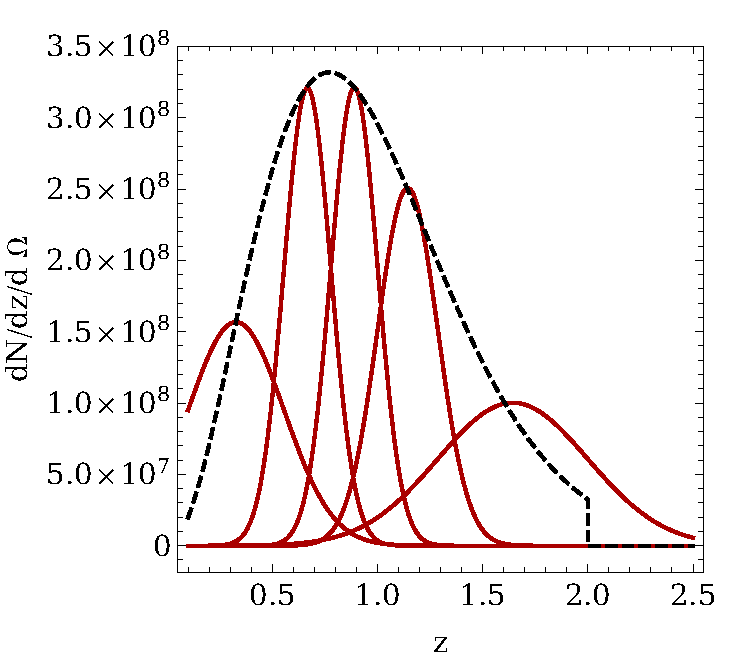
\includegraphics[width=\textwidth]{figures/chapter-mnu/euclid_5bin.pdf}
\end{center}
\caption{Euclid photometric galaxy density distribution (black line) with a division into 5 bins containing the same number of galaxies.
}
\label{fig:dNdz}
\end{figure}

%
\begin{figure}[hbtp]
\begin{center}
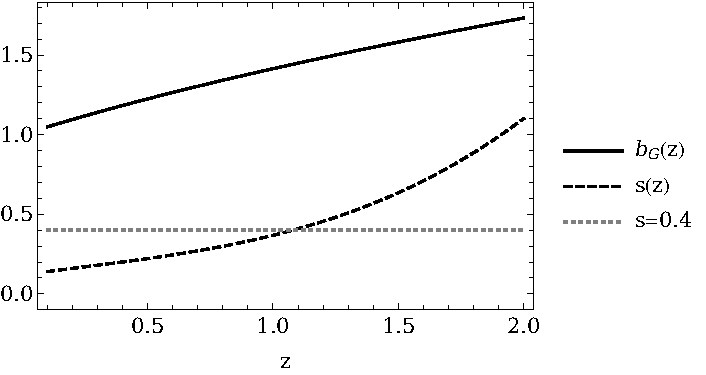
\includegraphics[width=\textwidth]{figures/chapter-mnu/bs.pdf}
\end{center}
\caption{Galaxy bias $b_G(z)$ and magnification bias $s(z)$ for Euclid. The
magnification bias is computed at the limiting magnitude $m_{\rm lim}=24.5$.
As a reference, we also plot the value $s=0.4$ at which the lensing contribution to number counts changes sign.
}
\label{fig:bs}
\end{figure}

Having the survey specifications we can compute angular matter power spectrum as in Eq. \eqref{Eq:binned-angular-matter-power-spectrum}. We have utilised the code CLASSgal \cite{DiDio:2013bqa} where galaxy number counts have been implemented including relativistic corrections in Eq. \eqref{Eq:galaxy-number-counts-perturbation}. In Figure \ref{Fig:comparison-massive-massless-Cls} we compare galaxy number counts angular power spectrum for a model with massive neutrinos and a model where neutrinos are massless. In the next section we study the importance of including the effect of lensing convergence in galaxy clustering analyses when determining the neutrino mass. 

\begin{figure}[hbtp]
\centering
%\includegraphics[scale=1]{}
\caption{\commentr{Include figure in two columns}Comparison auto and cross-corelations for models with and without neutrino mass}
\label{Fig:comparison-massive-massless-Cls}
\end{figure}
 
\section{Methodology}
\label{chapter-mnu:methodology}

In order to show how important the inclusion of lensing convergence in galaxy clustering analyses is, we perform a Markov Chain Monte Carlo (MCMC) analysis \cite{Lewis:2002ah,Verde:2003ey,Tegmark:2003ud} both including and neglecting the lensing effect. Studies analysing the bias on cosmological parameters due to neglecting lensing convergence can be found in the literature, but they do Fisher matrix analyses and focus on either the primordial non-Gaussianity parameter (i.e., $\fNL$) \cite{Namikawa:2011yr} or dark energy parameters (e.g., $w,\, \Omega_\Lambda$) \cite{Duncan:2013haa}. Although in this project we stress on the neutrino mass, we also discuss other parameters in the concordance model.  

The MCMC technique is more suitable than a Fisher matrix method. Current Boltzmann codes such as CLASS \cite{Lesgourgues:2011re} or CAMB \cite{Lewis:1999bs} are accurate to $1\%$ (with nominal precision settings), but it is possible for random numerical errors to exceed this. Future surveys will provide more precise Large Scale Structure (LSS) measurements and therefore these effects might become problematic for approaches that rely on computation of derivatives as a function of parameters (e.g., Fisher matrix). Since our MCMC approach average over $\sim 10^5$ galaxy number counts spectra, it is much less sensitive to those numerical errors than the Fisher matrix approach. 

We assume a fiducial flat $\Lambda CDM$ model consistent with results from the Planck collaboration \cite{Ade:2015xua}, including massive neutrinos with a normal mass hierarchy (dominated by the heaviest neutrino mass eigenstate). The cosmological parameters of our fiducial model are the reduced baryon density parameter, $\omega_{\mathrm{b}} = 2.225\times 10^{-2}$, the cold dark matter density parameter, $\omega_{\mathrm{cdm}}=0.1198$, the scalar spectral index, $n_{\mathrm{s}}=0.9645$, the amplitude of curvature fluctuations, $\ln 10^{10} A_{\mathrm{s}}=3.094$, the Hubble constant, $H_0 = 67.27\, \mathrm{km\, s^{-1}\, Mpc^{-1}}$, and the sum of the neutrino masses, $\sum m_\nu = 0.06\, \mathrm{eV}$.  
     
To take into account a theoretical error on non-linear scales we use Halofit \cite{Smith:2002dz} to rescale all linear transfer functions. The rescaling for the matter power spectrum in models including massive neutrinos has been already implemented in CLASSgal. Transfer functions are rescaled by the square root of 
\begin{equation}
\alpha(k,z) = \frac{\ln [1 + k/k_{\mathrm{NL}(z)}]}{1 + \ln [1 + k/k_{\mathrm{NL}(z)}]}f_{\mathrm{th}},
\label{Eq:rescaling-factor-transfer-functions}
\end{equation}
where $k_{\mathrm{NL}}$ is the non-linear scale determined by the Halofit algorithm, and $f_{\mathrm{th}}$ is the error percentage on non-linear scales that we have chosen to be $f_{\mathrm{th}}=10\%$. The theoretical error power spectra $E_\ell^{ij}$ are then computed by taking the absolute value of the resulting $C_\ell^{ij}$. Because computing $E_\ell^{ij}$ with high accuracy is time-computing demanding, in this project we compute the error power spectra only for the fiducial model, that is, we ignore the parameter dependence on the theoretical error. In addition, since the  perturbation on the number density of galaxies is not a continuous field, it is usually assumed that galaxies form a Poisson sample of the density field \cite{Feldman:1993ky} and therefore there is a shot-noise contribution $\N^{-1}$ to the error budget in the angular power spectra.

Finally, the galaxy number counts are modelled as 
\begin{equation}
\label{Eq:GNC-modelled-angular-power-spectra}
C_\ell^{A,\,ij} = C_\ell^{ij} + E_\ell^{ij} + \N^{-1} \delta^{ij},
\end{equation}
where $A=\mathrm{obs},\,\mathrm{th}$ and $i,j = 1,...,N_{\mathrm{bin}}$ are red-shift bin indices. Here $C_\ell^{\mathrm{obs}}$ stands for spectra computed for our fiducial model which includes the effect of lensing convergence, and $C_\ell^{\mathrm{th}}$ stands for models which might or might not include lensing convergence. In the next Section we will study the impact of switching lensing convergence off in $C_\ell^{\mathrm{th}}$ when fitting this kind of models to our fiducial $C_\ell^{\mathrm{obs}}$.   
     
Following the cosmic shear implementation in \cite{Audren:2012vy} we have implemented a Gaussian likelihood for an Euclid-like survey. For given observed and theoretical power spectra in Eq. \eqref{Eq:GNC-modelled-angular-power-spectra}, let us define the determinants
\begin{eqnarray}
\label{Eq:determinants-Gaussian-likelihood}
d_\ell^{\mathrm{th}} & = & \det \left( C_\ell^{\mathrm{th},\,ij}\right),\\
d_\ell^{\mathrm{obs}} & = & \det \left( C_\ell^{\mathrm{obs},\,ij}\right). 
\end{eqnarray}
Additionally, one can define a mixed determinant $d_\ell^{\mathrm{mix}}$ formed from $d_\ell^{\mathrm{th}}$: one takes each term in $d_\ell^{\mathrm{th}}$ and replaces one at a time $C_\ell^{\mathrm{th},\,ij}$ by the corresponding $C_\ell^{\mathrm{obs},\,ij}$. If we worked with $2$ red-shift bins, the mixed determinant would read
\begin{equation}
\label{Eq:example-mixed-determinant}
d_\ell^{\mathrm{mix}} = C_\ell^{\mathrm{obs},\,11}C_\ell^{\mathrm{th},\,22} + C_\ell^{\mathrm{th},\,11}C_\ell^{\mathrm{obs},\,22} - 2 C_\ell^{\mathrm{th},\,12}C_\ell^{\mathrm{obs},\,12}.
\end{equation}
                        
It is known that in an ideal full-sky experiment, the different multipoles in an spherical harmonics expansion of a given function are uncorrelated. Then in this simple case one can write the Gaussian likelihood
\begin{equation}
\label{Eq:GNC-Gaussian-likelihood}
\L = \widetilde{\N} \Pi_\ell \left\lbrace \frac{1}{(d_\ell^{\mathrm{th}})^{\frac{2\ell+1}{2}}} \exp \left[ -\frac{(2\ell+1)}{2} \frac{d_\ell^{\mathrm{mix}}}{d_\ell^{\mathrm{th}}}\right] \right\rbrace,                         
\end{equation}
where $\widetilde{\N}$ is a normalisation constant. The effective chi square is defined as
\begin{equation}
\label{Eq:GNC-effective-chi2}
\chi^2_\eff \equiv -2 \ln \L = -2 \ln \widetilde{\N} + \sum_\ell (2\ell+1)\left( \ln d_\ell^{\mathrm{th}} + \frac{d_\ell^{\mathrm{mix}}}{d_\ell^{\mathrm{th}}} \right), 
\end{equation}
which is minimal for $d_\ell^{\mathrm{mix}}= N_{\mathrm{bin}} d_\ell^{\mathrm{th}} = N_{\mathrm{bin}} d_\ell^{\mathrm{obs}}$. Having into account the partial sky coverage these definitions lead to a $\chi^2$ relative to the fiducial model given by                     
\begin{equation}
\label{Eq:relative-chi2}
\Delta \chi^2 = \sum_{\ell=2}^{\ell_{\mathrm{max}}} (2\ell+1) f_\fsky \left( \ln \frac{d_\ell^{\mathrm{th}} }{d_\ell^{\mathrm{obs}}} + \frac{d_\ell^{\mathrm{mix}}}{d_\ell^{\mathrm{th}}} - N_{\mathrm{bin}} \right),
\end{equation}                           
where to be conservative in the treatment of non-linear effects we use $\ell_{\mathrm{max}}=400$. In order to optimise the computation of the angular power spectra $C_\ell^{\mathrm{A},\,ij}$ we use the Limber approximation and adjust the precision parameters in CLASSgal to have $\Delta \chi^2 \lesssim 0.2$ for $C_\ell^{\mathrm{th}}$ including lensing evaluated at the fiducial model. These adjustments are necessary to make feasible our MCMC approach and mean that our computations are accurate up to $\Delta \chi^2 \lesssim 0.2$.                              
                                                                      
\section{Results}
\label{chapter-mnu:results}

Utilising the approach explained in Section \ref{chapter-mnu:methodology}, we have performed the three following MCMC  analyses:

\begin{enumerate}
\item $C_\ell^{\mathrm{th}}$ including lensing convergence.
\item $C_\ell^{\mathrm{th}}$ neglecting lensing convergence.
\item $C_\ell^{\mathrm{th}}$ neglecting lensing convergence, but including only auto-correlations.
\end{enumerate}

We have done these analyses in two ways. First, we assume no previous information and use wide, flat prior distributions for the cosmological parameters. Second, we consider a more realistic scenario where information from a full-sky CMB experiment is provided. In this case we assume a Gaussian prior distribution for the pertinent cosmological parameters; we compute the covariance matrix for a model with varying neutrino mass from information provided by the Planck collaboration. In addition to these two analyses, we do a Fisher matrix analysis no using priors and compare results with the corresponding MCMC analysis. We close this section by estimating the significance of lensing detection with an Euclid-like survey.

\subsection{MCMC with wide, flat priors}

The Figure \ref{fig:mcmc} shows two- and 1-D posteriors for the three mentioned analyses using wide, flat priors on the cosmological parameters. The corresponding constraints are shown in Table \ref{Table:1}. Red contours indicate results for the analysis that consistently includes lensing convergence in the theoretical model fitting the mock data. The analysis neglecting lensing convergence, but including only red-shift bin auto-correlations (i.e.\ $C_\ell(z,z)$), is depicted in gray. Blue contours show the analysis neglecting lensing, but including all possible red-shift bin correlations (i.e.\ $C_\ell(z,z')$).      

% \begin{table}[!tbhp]
\begin{table}[!t]
  \centering
  \begin{tabular}{@{}cccccc}
    \hline
    \multicolumn{6}{c}{i) Consistently including lensing: $\Delta \chi^2 = 0$} \\
    \hline
    Parameter & Mean & best fit & $\sigma$ &\hspace{-0.52cm} shift: mean & best-fit \\
    \hline
    $\omega_b$ & $0.02979$ & $0.02285 $ &$0.00624 $ &  \quad$1.2\sigma$ & $ 0.1\sigma$ \\
    $\omega_{cdm}$ & $0.1455 $ & $0.1219 $ & \quad$0.0200 $ &  \quad$1.3\sigma$ & $0.1\sigma$ \\
    $n_s$      & $0.9476 $ & $0.9642 $ & $0.0387 $ &  \quad$0.4\sigma$ & $ <0.1\sigma$ \\
    $\ln10^{10}A_s$ & $3.047 $ & $3.097$ & $0.065 $ &  \quad$0.7\sigma$ & $ <0.1\sigma$ \\
    $H_0\left[\frac{\text{km}}{\text{s}\cdot\text{Mpc}}\right]$      & $73.84$ & $67.84$ & $5.48$ &  \quad$1.2\sigma$ & $ 0.1\sigma$ \\
    $m_{\nu}$\,[eV]  & $0.29$ & $0.09$ & $0.19$ & \quad $ 1.2\sigma$ & $ 0.2\sigma$ \\
    $b_0$ & $1.018$ & $1.000$ & $0.031$ & \quad$0.6\sigma$ & $<0.1\sigma$ \\
  \end{tabular}
  \begin{tabular}{@{}cccccc}
    \hline
    \multicolumn{6}{c}{ii) Neglecting lensing: $\Delta \chi^2 = 2064$} \\
    \hline
    Parameter & Mean & best fit & $\sigma$ & \hspace{-0.52cm} shift: mean & best-fit \\
    \hline
    $\omega_b$ & $0.02494$ & $0.02120 $ & $0.00556 $ &  \quad$0.5\sigma$ & $0.1\sigma$ \\
    $\omega_{cdm}$ & $0.1532$ & $0.1435$ & $0.0208$ &  \quad$1.6\sigma$ & $1.1\sigma$ \\
    $n_s$      & $0.8702$ & $0.8837$ & $0.0446$ &  \quad$2.1\sigma$ & $1.8\sigma$ \\
    $\ln10^{10}A_s$ & $ 2.867 $ & $2.965 $ & $ 0.394 $ &  \quad$0.6\sigma$ & $0.3\sigma$ \\
    $H_0\left[\frac{\text{km}}{\text{s}\cdot\text{Mpc}}\right]$      & $68.73$ & $66.76$ & $5.14$ &  \quad$0.3\sigma$ & $0.1\sigma$ \\
    $m_{\nu}$\,[eV]  & $0.43$ & $0.41$ & $0.16$ &  \quad$2.3\sigma$ & $2.2\sigma$ \\
    $b_0$ & $1.293$ & $1.200$ & $0.271$ & \quad$1.1\sigma$ & $0.7\sigma$\\
  \end{tabular}
  \begin{tabular}{@{}cccccc}
    \hline
    \multicolumn{6}{c}{\parbox[t]{4.4cm}{iii) Neglecting lensing: \\ \hspace*{0.9cm} (only auto-correlations)} $\Delta \chi^2 = 180$} \\
    \hline
    Parameter & Mean & best fit & $\sigma$ & \hspace{-0.52cm} shift: mean & best-fit\\
    \hline
    $\omega_b$ & $0.01982 $ & $0.01737 $ & $0.00520 $ &  \quad$0.5\sigma$ & $0.9\sigma$ \\
    $\omega_{cdm}$ & $0.1658 $ & $0.1552 $ & $0.0242 $ &  \quad$1.9\sigma$ & $1.5\sigma$ \\
    $n_s$      & $0.7539 $ & $0.7675 $ & $0.0513 $ &  \quad$4.1\sigma$ & $3.8\sigma$ \\
    $\ln10^{10}A_s$ & $2.449 $ & $2.719 $ & $0.465 $ &  \quad$1.4 \sigma$ & $0.8\sigma$ \\
    $H_0\left[\frac{\text{km}}{\text{s}\cdot\text{Mpc}}\right]$      & $61.64 $ & $59.11$ & $5.43$ &  \quad$1 \sigma$ & $1.5\sigma$ \\
    $m_{\nu}$\,[eV]  & $0.41$ & $0.41$ & $0.14$ &  \quad$2.6\sigma$ & $2.5\sigma$ \\
    $b_0$ & $1.888$ & $1.603$ & $0.428$ & \quad$2.1\sigma$ & $1.4\sigma$ \\
  \end{tabular}

  \caption{MCMC results (flat prior). We show the mean and best fit values, the standard deviation and the amplitude of the shift of the mean and best-fit w.r.t the fiducial value in units of the standard deviation, $\sigma$, of the corresponding analysis. The large value of $\Delta \chi^2$ for case ii) shows that cross-correlations cannot be fitted if lensing is neglected.  A shift of less than about $0.2\sigma$ is not serious and probably due to the reduced precision used to compute the theoretical spectra.}
  \label{Table:1}
\end{table}

\begin{figure*}[bthp]
  \centering
  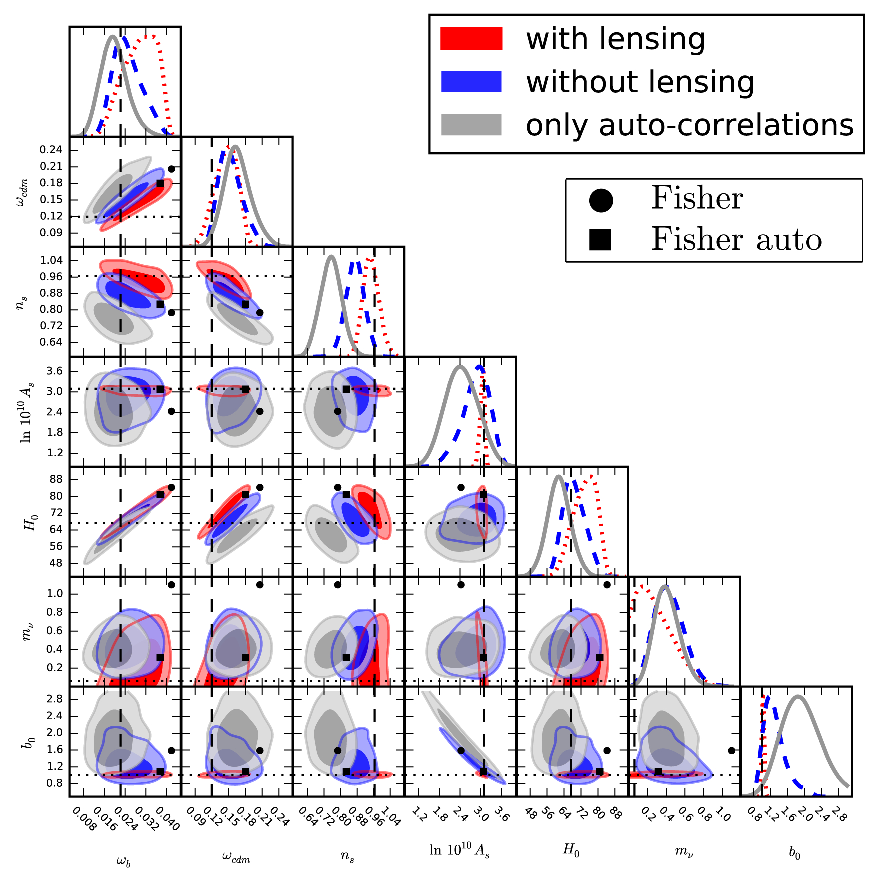
\includegraphics[width=\textwidth]{figures/chapter-mnu/triangle_figure_MCDM_bias_w_legend.pdf}
  \caption{Two- and 1-D posteriors for the cosmological parameters inferred from the full analysis including lensing (red dotted), an analysis neglecting lensing (blue dashed) and considering only auto-correlations (gray solid).
    The 68\% and 95\% confidence intervals are shown.
    Intersections between vertical and horizontal lines denote the fiducial cosmology.
   In this analysis no significant priors were imposed on the parameters.  Circles and squares represent the estimates for the best-fits from a Fisher matrix analysis when neglecting lensing, and for the only auto-correlations case, respectively.
  }
  \label{fig:mcmc}
\end{figure*}

%We have  fitted the generated $C_\ell^{ij}$ data in three different ways,  where lensing convergence is: i) consistently included, ii) neglected, iii) neglected and only redshift bin auto-correlations are taken into account. 

%The results are shown in Table~\ref{Table:1} and Figure~\ref{fig:mcmc}. Fig.~\ref{fig:mcmc} shows 2D contours and 1D probability distribution functions for the marginalized posteriors of the cosmological parameters obtained from these analyses. The red contours (dotted 1D distributions) show the full analysis. They should reproduce the fiducial model. In the analyses shown by the gray (1D solid) and blue (1D dashed) contours lensing is neglected. Furthermore, in the gray  contours only auto-correlations (i.e.\ $C_\ell(z,z)$) are considered, while the blue contours use both auto- and cross-correlations (i.e.\ $C_\ell(z,z')$ for all combinations of redshift bins).
%The auto-correlation case is closer to the standard $P(k)$ analysis which is usually performed in redshift bins, but caution should be taken in comparing the two analyses since binning in redshift has significantly different effects.

The analysis that consistently includes lensing convergence (red contours in Figure \ref{fig:mcmc}) should output the fiducial model. The corresponding constraints in Table \ref{Table:1} show that the best fitting parameters are indeed very close to the input fiducial parameters (see the amplitude of the shift of the best fit). The amplitude of the shifts of the mean of some parameters (i.e., $m_\nu$, $H_0$, $\omega_{cdm}$, $\omega_b$) reveal the limitations of our analysis. On the one hand, since the main impact of massive neutrinos occurs on small scales and we treat non-linear scales very conservatively, an improvement on the constraints of the neutrino absolute mass scale is expected in an analysis including, for instance, scales up to $\ell=2000$. On the other hand, the universe's expansion rate, the reduced baryon density parameter, and the cold dark matter density parameter are not well constrained due to degeneracies in these parameters (see Figure \ref{fig:mcmc}). These degeneracies come from the dominant contributions in the matter transfer function that are basically fixed by the ratio $\omega_b/\omega_{\mathrm{cdm}}$ and by the scale of the particle horizon at the radiation-matter equality epoch $z_{\mathrm{eq}}$ \cite{Eisenstein:1997ik}. The equality scale $k_{\rm eq}$ behaves like  
\begin{equation}
k_{\rm eq} \propto \frac{\omega_m}{H_0},
\end{equation}      
where we assume a fixed radiation content and measure $k_{\rm eq}$ in $h/ \Mpc$.  
%From the red contours in Fig.~\ref{fig:mcmc} it is evident that we cannot determine the baryon and cold dark matter densities very well with our configuration. The rather large redshift bins of our analysis with $\Delta z\gtrsim 0.3$ significantly smear out the baryon acoustic oscillations (BAO's), leaving only the dominant features in the power spectrum which are fixed by the equality scale, $k_{\rm eq} \propto \omega_m/H_0$ (at fixed radiation content and measured in $h/$Mpc) and the ratio $\omega_b/\omega_{\mathrm{cdm}}$. This  leads to a significant  degeneracy between $\omega_b$, $\omega_{\rm cdm}$ and $H_0$, only the slopes of the $(\omega_x,H_0)$ and the $(\omega_b, \omega_{\rm cdm})$  contours are well determined. The large uncertainties in these parameters, as well as the prior $m_\nu\geq 0$, push the posterior mean value away from the best fit (which is always very close to the input value). We did not add realization noise in our likelihood, since it is not relevant for the present study.
%Our aim here is not to derive optimal parameter constraints, but to demonstrate the importance of the lensing contribution in such an analysis. For this reason our approach is far from optimal but  conservative and simple, and even in this case we find that not including lensing leads to wrong results.
%Optimizing error contours by, e.g., introducing more non-linear scales in the analysis is expected to lead to even more biased results, given  that  the relevance of lensing increases at higher multipoles.

Gray contours in Figure \ref{fig:mcmc} show the analysis neglecting lensing, but including only red-shift bin auto-correlations. The effective $\Delta \chi^2$ for this case is greater than in the case consistently including lensing, thus suggesting that the model neglecting lensing has difficulties in fitting the mock data. The spectral index and the neutrino mass are significantly biased ($>2.5\sigma$) from the input fiducial parameters. Moreover, a degeneracy between the bias parameter $b_0$ and the amplitude of scalar fluctuations $A_s$ appears. This comes from the fact that the product $A_s b_0^2$ determines the overall amplitude of matter fluctuations and therefore its increase (decrease) signifies an enhancement (decrement) of power on all scales. The bias on $n_s$ and $m_\nu$ can be understood as follows. Since the magnification bias in $s(z)$ Eq. \eqref{Eq:magnification-bias} is relatively large (see Figure \ref{fig:bs}), the density-lensing correlation term
\begin{equation}
b(z)(5s(z)-2)\langle D \kappa \rangle,
\end{equation}   
contributes to the power with a positive (negative) sign for red-shift bins with $z>1$ ($z<1$). Because correlations of relatively small red-shifts bins probe mainly small scales, the decrement of power on small scales due to lensing convergence must be corrected in a model no including lensing. This correction can be achieved by lowering the spectral index -- since $P(k) \propto k^{n_s -1}$ -- and increasing the neutrino mass.

Finally, we focus our attention on the analysis that neglects lensing convergence, but includes all red-shift bin correlations (blue contours in Figure \ref{fig:mcmc}). Although bias on cosmological parameters appear to be smaller in this case -- as compared to the gray contours --, this improvement is not significant. Since the lensing term might actually dominate the radial power spectrum at large scales \cite{Bonvin:2011bg}, it is even more difficult for a model that neglects lensing and includes cross-correlations to fit the mock data. This is easily seen with the value of the effective $\Delta \chi^2$ in Table \ref{Table:1}. The $\Delta \chi^2$ increases from $\Delta \chi_{\rm auto}^2\simeq 180$ for the five auto-correlation bins to more than $\Delta \chi_{\rm a+c}^2\gtrsim2000$ when adding the 10 cross-correlation bins. If one naively gives each bin the same weight,  one would expect an increase by a factor 3. We however find an increase
$\Delta \chi_{\rm a+c}^2/\Delta \chi_{\rm auto}^2\gtrsim 11$.   

Models with additional parameters, but neglecting lensing convergence are likely to weaken the constraints -- introducing new degeneracies -- and produce even stronger biases on the cosmological parameters. Therefore, from the analyses presented above, we conclude that to go beyond the current state and derive accurate estimates of the absolute neutrino mass scale with galaxy surveys absolutely requires taking lensing convergence into account. Figure \ref{fig:cl}   shows number counts angular power spectra for analyses including and neglecting lensing computed at the corresponding best fit (see Table \ref{Table:1}). The thick red lines indicate the model including lensing and the thin blue lines show the model neglecting lensing (including all red-shift bin cross-correlations). For the spectra of the model consistently including lensing, we show 1-$\sigma$ error bars that were computed by assuming Gaussian spectra (see Eq.~(2.13) of \cite{Montanari:2015rga}). Correlations between the red-shift bins $(ij)=(11), ~(55)$ and $(15)$ are shown. One can see that when neglecting lensing, the spectrum for the cross-correlation between red-shift bins $1$ and $5$ lies outside the 1-$\sigma$ error bars around the fiducial spectrum including lensing. This clearly evidences that a  model neglecting lensing convergence cannot fit the mock data.

%If lensing is neglected in the analysis, several parameters
%show a significant bias with respect to the input parameters (given by the vertical dashed lines)  cf. also Table~\ref{Table:1}.
%First of all, there is a very strong degeneracy between the scalar amplitude $A_s$ and the bias $b_0$.  When including lensing which does not depend on $b_0$ this degeneracy is broken and both, $b_0$ and $A_s$ are determined accurately. Furthermore, lensing (together with the magnification bias for Euclid specifications) enhances clustering. Compensating this with a larger value of $b_0^2A_s$ leads to too much clustering on small scales, which, in turn, is compensated by reducing the spectral index by $(2-4)\sigma$ and by increasing the neutrino mass.   The preferred neutrino mass
%is around $0.4\, \mathrm{eV}$, which corresponds just about to the current limits from cosmology~\cite{Ade:2015xua}.
%From the degeneracy directions in the two-dimensional contours in Fig.~\ref{fig:mcmc}
%we can also read off that forcing $m_\nu \rightarrow m_\nu^{\rm (fid)} = 0.06\, \mathrm{eV}$ would lead to
%an even larger bias in the scalar spectral index.


%It is interesting that taking cross-correlations into account helps somewhat to reduce the bias on the parameters. The scalar spectral index best-fit in this case has a bias of $1.8\sigma$,  as compared to $3.8\sigma$ for auto-correlations only, and the neutrino mass is shifted by $2.2 \sigma$ compared to $2.5\sigma$,
%see Table~\ref{Table:1}. But this `improvement' is actually not real. It comes to a big extent from the fact that cross-correlations simply cannot be fitted without the lensing term as discussed below and shown in Fig.\ \ref{fig:cl}.  This is most manifest in the  total $\Delta \chi^2$ which increases from $\Delta \chi_{\rm auto}^2\simeq 180$ for the five auto-correlation bins to more than $\Delta \chi_{\rm a+c}^2\gtrsim2000$ when adding the 10 cross-correlation bins. Giving each bin naively the same weight we would expect an increase by a factor 3, instead we have
%$\Delta \chi_{\rm a+c}^2/\Delta \chi_{\rm auto}^2\gtrsim 11$.
%The increase in the size of the parameter contours for some parameters appears at first counter-intuitive as including more data improves our knowledge and therefore should reduce the errors.
%This simple logic, however, only applies if the data can actually be fitted by the model at hand or if the likelihoods are Gaussian. Otherwise, different data may prefer different model parameters and lead to an increase not only in the total $\Delta \chi^2$ but also in the size of the confidence contours.



\begin{figure}[tp]
  \centering
  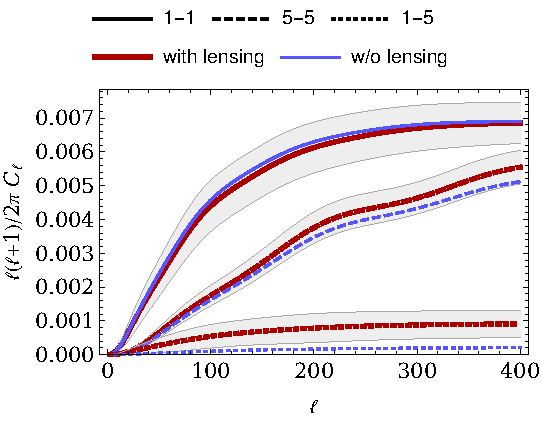
\includegraphics[width=\columnwidth]{figures/chapter-mnu/fid_shift.pdf}
  \caption{
    The thick red and the thin blue lines correspond to the spectra at the best-fit values estimated by consistently including lensing and by neglecting it, respectively.
    Gaussian error bars accounting for cosmic variance and shot-noise for the consistent analysis are shown as gray regions.
    The indices for the correlated redshift bins are shown in the legend.
    The model neglecting lensing cannot fit the data, especially due to redshift cross-correlations.
  }
  \label{fig:cl}
\end{figure}


\begin{table}[!t]
  \centering
  \begin{tabular}{c|cccc}
    Parameter & \multicolumn{2}{c}{Shift of best-fit } &\multicolumn{2}{c}{for MCMC} \\
    \hline
       $\omega_b$ & $1.2\sigma$ & ($0.9\sigma$) & $-0.1\sigma$ & ($-0.9\sigma$)\\
   $\omega_{cdm}$ & $1.7\sigma$ & ($1.1\sigma$)& $1.1\sigma$ &
($1.5\sigma$)\\
   $n_s$      & $-1.9\sigma$ & ($-1.3\sigma$) & $-1.8\sigma$ &
($-3.8\sigma$) \\
   $\ln10^{10}A_s$ & $-1.1\sigma$ & ($0.005\sigma$)& $-0.3\sigma$ &
($-0.8\sigma$)\\
   $H_0\left[\frac{\text{km}}{\text{s}\cdot\text{Mpc}}\right]$ &
$1.2\sigma$ & ($0.9\sigma$)& $-0.1\sigma$ & ($-1.5\sigma$)\\
   $m_{\nu}$\,[eV]  & $3.3\sigma$ & ($0.6\sigma$)  & $2.2\sigma$ &
($2.5\sigma$)\\
   $b_0$      & $1.7\sigma$ & ($0.1\sigma$)   & $0.7\sigma$ &
($1.4\sigma$)\\
  \end{tabular}

  \caption{
      Fisher matrix results for the shift in the best-fit values due to neglecting lensing, in units of standard deviations (see Figure \ref{fig:fisher}). The numbers in parenthesis refer the the case including only bin auto-correlations. For comparison we also give in columns 4 and 5 the corresponding values from the MCMC analysis presented in Table~\ref{Table:1} and Fig.~\ref{fig:mcmc}. While Fisher matrices give a good qualitative description of parameter degeneracies, estimates of the shifts in the best-fits seriously misestimate the magnitude and direction in parameter space.
 }
  \label{Table:Fisher}
\end{table}

\begin{figure*}[bthp]
  \centering
  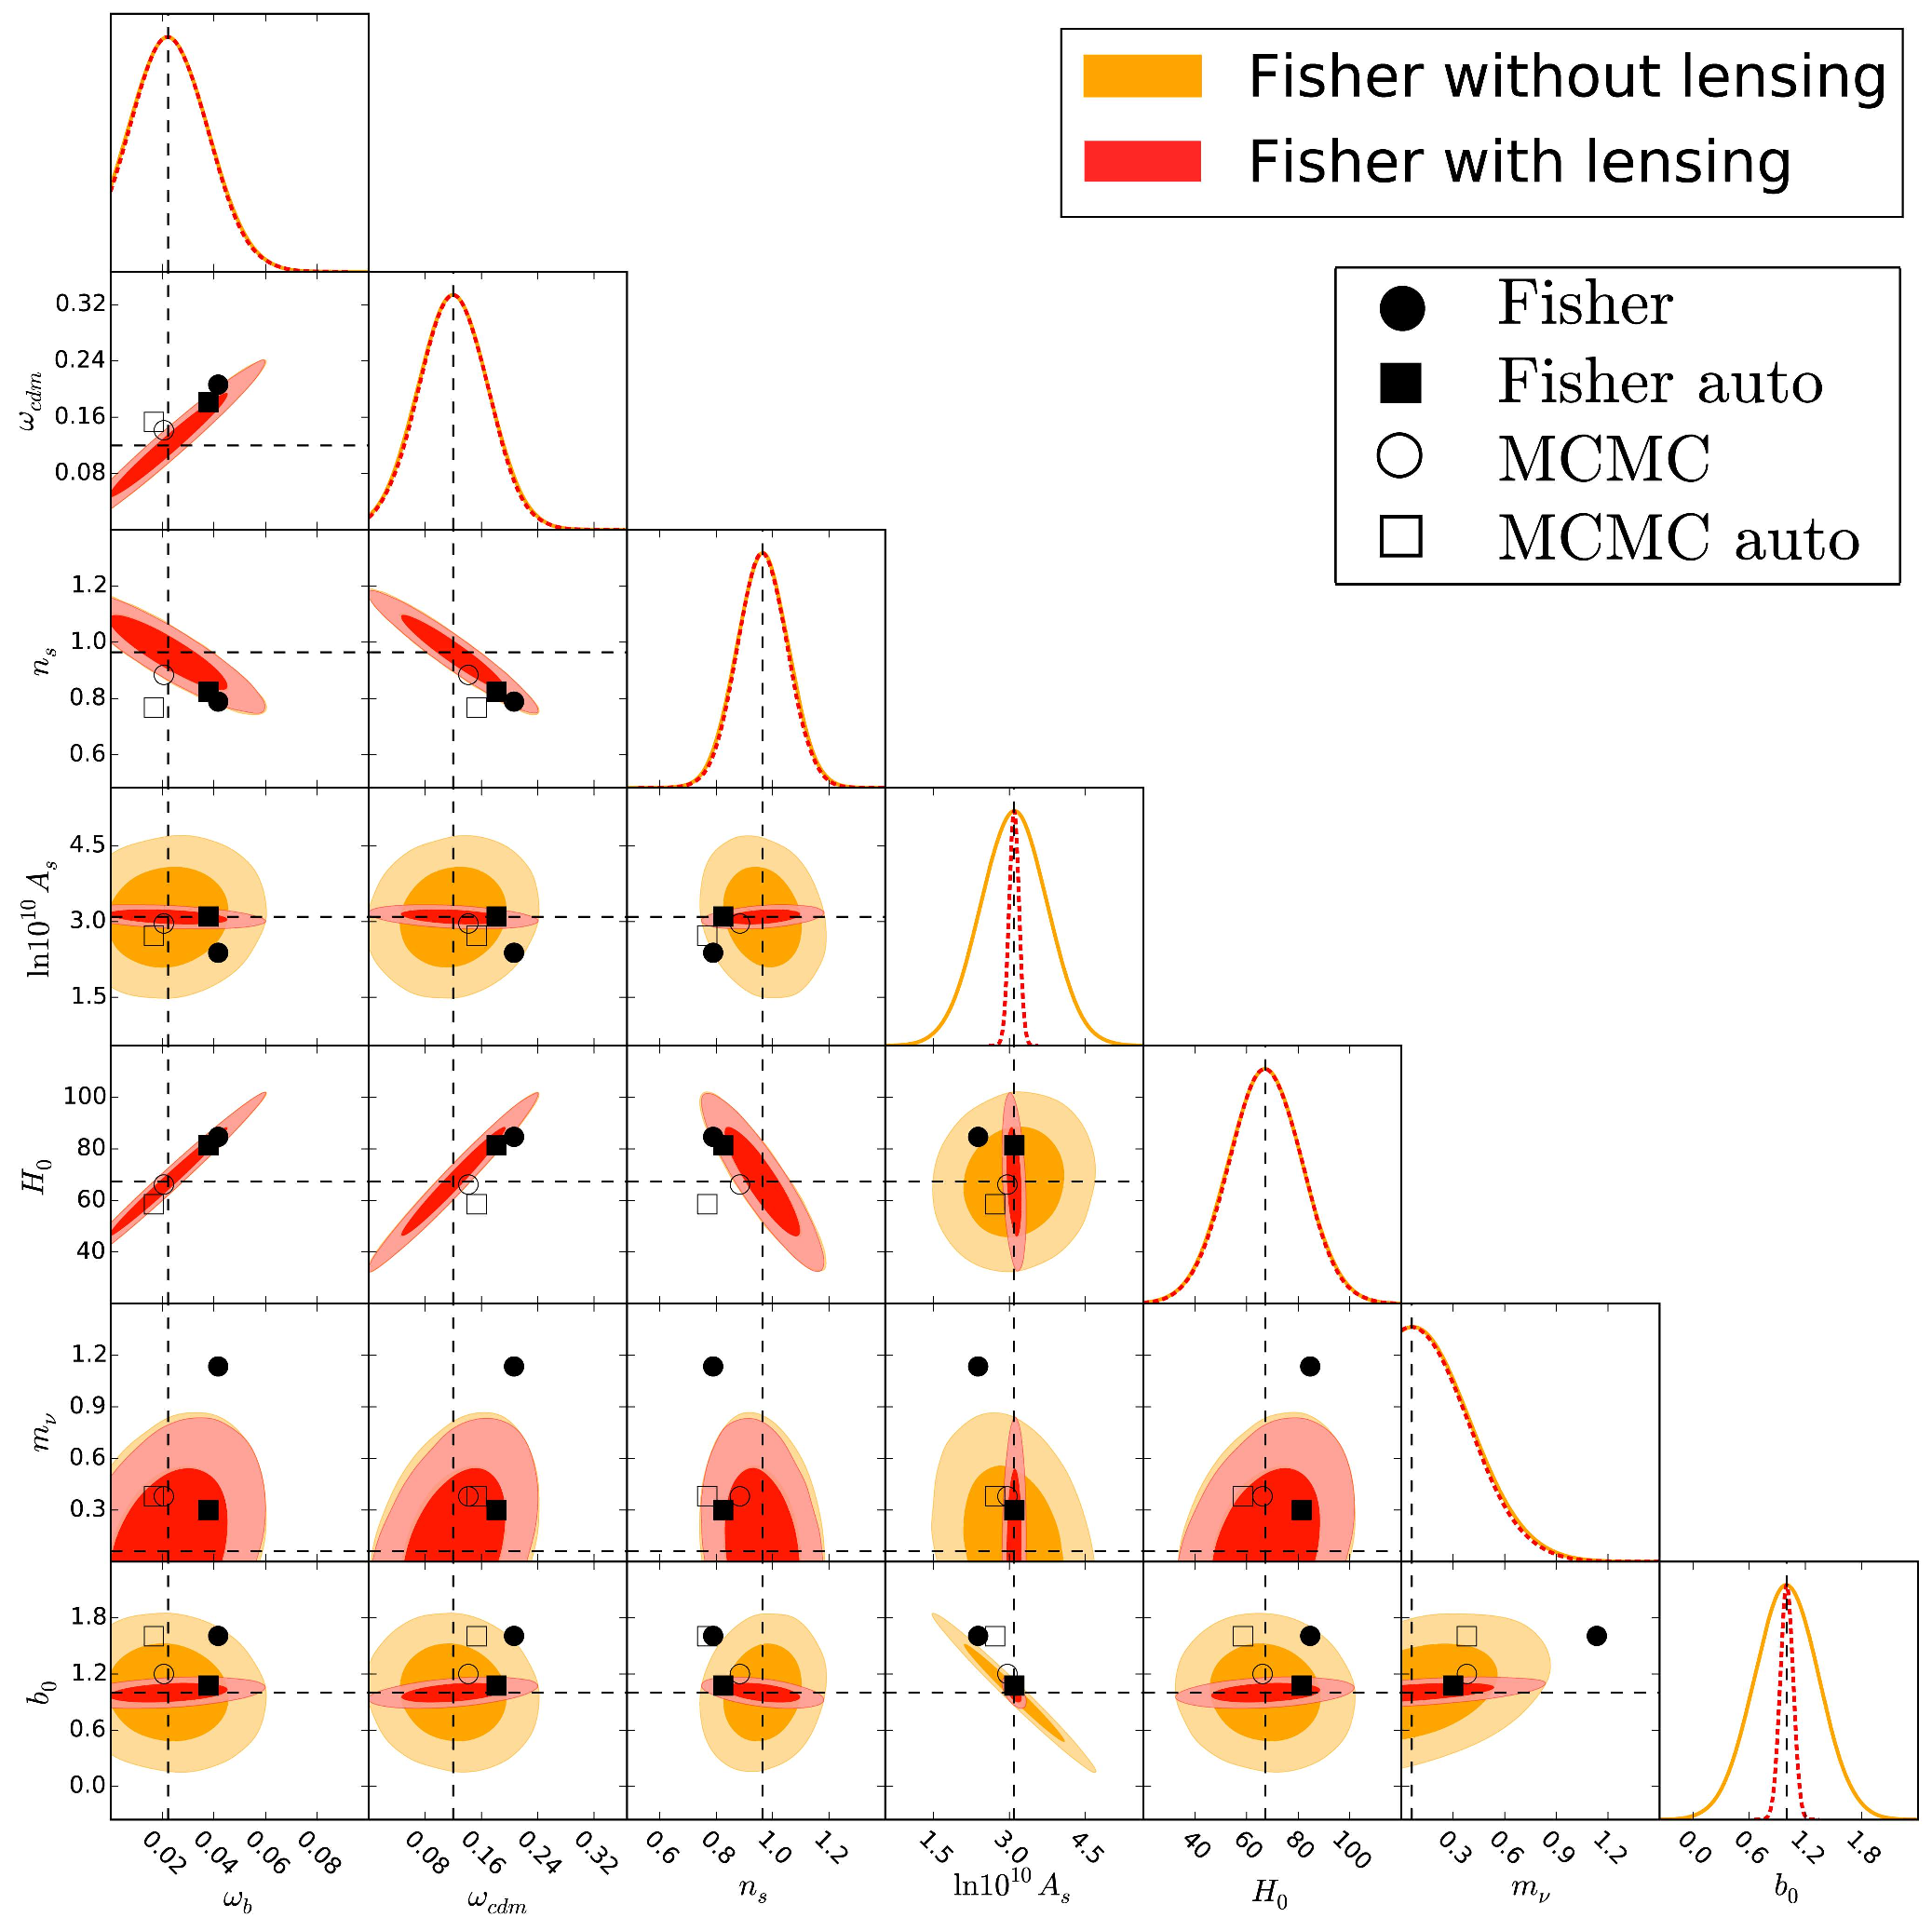
\includegraphics[width=\textwidth]{figures/chapter-mnu/triangle_figure_Fisher_bias.pdf}
  \caption{
      Two- and 1-D posteriors for the cosmological parameters inferred from the Fisher analysis excluding (orange solid) and including lensing (red dotted).
    We stress that, in the former case, to compute error ellipses within the Fisher formalism we forecast parameter constraints in a Universe where lensing is absent (see the text for more details).
    The 68\% and 95\% confidence intervals are shown.
    Intersections of dashed lines denote the fiducial cosmology.
The expected systematic shifts in the best-fit due to neglecting lensing in the theoretical modeling are shown, including all bin correlations (circles), and including only auto-correlations (squares).
For comparison, we also show the corresponding results from the MCMC analysis.
While the Fisher formalism is reliable for a qualitative understanding of parameter degeneracies, the systematic errors are seriously misestimated.
    See table \ref{Table:Fisher} for more details about statistical quantities.
}
  \label{fig:fisher}
\end{figure*}

\subsection{Fisher analysis without priors}\label{s:fisher}

The shift of best fit parameters  and the change in the figure of merit due to neglecting relativistic corrections (hence, in particular, neglecting lensing) has been studied previously, see e.g.~\cite{Namikawa:2011yr,Duncan:2013haa,Camera:2014sba,Raccanelli:2015vla}. However, these previous works did not include massive neutrinos and they used a Fisher matrix analysis which gives quantitative estimates for shifts only if these are significantly less than one standard deviation.
Hence the results obtained in these works can only be trusted qualitatively while the MCMC study presented here gives quantitative results and demonstrates that large biases, exceeding by far $1\sigma$, are to be expected even for not very ambitious survey specifications.

We illustrate this here by repeating our analysis with a Fisher matrix technique.
The results are presented in Figure \ref{fig:fisher}, where we also show the shifts of the best fit values estimated via Fisher matrices (see appendix~\ref{app:fisher} for details).
  Fisher matrix contours are reported for both cases, without and including lensing.
  This information is also reported in Table \ref{Table:Fisher}, where the standard deviations, $\sigma$, refer to the case without lensing, which provides more conservative information about the importance of the systematic error.
  We stress that in both cases, without and with lensing, Fisher matrices only forecast error contours around a universe described by the fiducial parameters and assume a Gaussian likelihood.
  While the MCMC analysis allows us to fit the wrong or the correct model to the data, in the Fisher context this is not possible.
  E.g., in the case without lensing we ask the outcome of fitting a model without lensing to a Universe without lensing.
  Hence, while the red dotted contours `with lensing' can be compared between Figures \ref{fig:mcmc} and \ref{fig:fisher}, the other contours have no correspondence between the two figures.
  In our case Fisher matrices provide a good qualitative description of degeneracy between different parameter constraints. The 68\% confidence intervals are in disagreement with MCMC results by a factor 2-3, but the shape and inclination of the ellipses very roughly follow the MCMC contours.
  However, the magnitude and direction of the best-fit shift in parameter space due to neglecting lensing is seriously misestimated.
  Indeed, the first-order formalism that we use to estimate the shift in the best-fits due to a systematic error is only valid to the extent that the shift is small compared to the errors (error contours are themselves meaningful only close enough to the fiducial cosmology), and also assuming that the systematic error does not affect the ellipse contours \cite{Kitching:2008eq}.
  Neither of these conditions is actually satisfied.

\subsection{MCMC with Planck Gaussian prior}

A more realistic analysis makes use of prior knowledge of parameters from previous experiments. We therefore
repeat our MCMC analysis using Planck priors for all the cosmological parameters except the bias, which is not measured in {\it Planck}, and the neutrino mass. The latter is our most interesting parameter and we want to test how strongly it is biased in an analysis which neglects lensing.

{\it Planck} chains are publicly available through the \textit{Planck Legacy Archive}. In this paper we use the chain for the extended model with a free neutrino mass based on the {\it Planck} TT, TE, EE + lowP likelihoods (Equation [54c] in \cite{Ade:2015xua}). We compute the covariance matrix $\mathbf{C}$ for the cosmological parameters $\vec{x}=(\omega_b,\omega_{\mathrm{cdm}},n_s,A_s,H_0)$ and assume a Gaussian distribution for the prior. The $\chi^2$ relative to the fiducial model including the Planck prior is then the $\Delta \chi^2$ in Eq. \eqref{eq:chi2} plus
\begin{equation}
\Delta \chi^2_{\mathrm{prior}} = \sum_{i,j} (x_i - x^{\mathrm{fid}}_i)^2 C^{-1}_{ij} (x_j - x^{\mathrm{fid}}_j)^2,
\label{Eq:chi2-prior}
\end{equation}
where $\vec{x}^{\mathrm{fid}}$ denotes parameters of the fiducial model and $\mathbf{C^{-1}}$ is the inverse of the covariance matrix.
In this way we marginalize the Planck prior over the neutrino mass and the optical depth, $\tau$, which are parameters that we want to leave free since we want to determine the first and our survey is not sensitive to the second. The results are shown in Table~\ref{Table:2} and Fig.~\ref{fig:mcmc-cmb-prior}.


Cosmological parameters in this case are clearly better determined than for the case without priors.
While the spectral index $n_s$ shows now a smaller relative shift, the neutrino masses and galaxy bias actually acquire larger shifts.
The incompatibility of data and model pulls the Hubble parameter $H_0$ away from the fiducial value by over $4\sigma$ in spite of the Planck prior.
Hence, while the details of the analysis are important in determining the actual size of error bars and degeneracies in parameter space, a large bias $2\sigma$--$9\sigma$ in the neutrino masses is a feature that persists in all the analyses here performed.


\begin{table}[!t]
  \centering
  \begin{tabular}{@{}cccccc}
    \hline
    \multicolumn{6}{c}{i) Consistently including lensing: $\Delta \chi^2 = 0$} \\
    \hline
    Parameter & Mean & best fit & $\sigma$ &\hspace{-0.52cm} shift: mean & best-fit \\
    \hline
    $\omega_b$ & $0.02223$ & $0.02226 $ &$0.00013 $ &  \quad$0.2\sigma$ & $ <0.1\sigma$ \\
    $\omega_{cdm}$ & $0.1200 $ & $0.1196 $ & \quad$0.0011 $ &  \quad$0.2\sigma$ & $0.2\sigma$ \\
    $n_s$      & $0.9642 $ & $0.9651 $ & $0.0041 $ &  \quad$0.1\sigma$ & $ 0.1\sigma$ \\
    $\ln10^{10}A_s$ & $3.092 $ & $3.098$ & $0.026 $ &  \quad$0.1\sigma$ & $ 0.2\sigma$ \\
    $H_0\left[\frac{\text{km}}{\text{s}\cdot\text{Mpc}}\right]$      & $67.08$ & $67.25$ & $0.70$ &  \quad$0.3\sigma$ & $ <0.1\sigma$ \\
    $m_{\nu}$\,[eV]  & $0.08$ & $0.04$ & $0.05$ & \quad $ 0.4\sigma$ & $ 0.4\sigma$ \\
    $b_0$ & $1.005$ & $0.994$ & $0.018$ & $0.3\sigma$ & $0.3\sigma$ \\
  \end{tabular}
  \begin{tabular}{@{}cccccc}
    \hline
    \multicolumn{6}{c}{ii) Neglecting lensing: $\Delta \chi^2 = 2082$} \\
    \hline
    Parameter & Mean & best fit & $\sigma$ & \hspace{-0.52cm} shift: mean & best-fit \\
    \hline
    $\omega_b$ & $0.02220$ & $0.02219 $ & $0.00017 $ &  \quad$0.3\sigma$ & $0.4\sigma$ \\
    $\omega_{cdm}$ & $0.1215$ & $0.1214$ & $0.0014$ &  \quad$1.2\sigma$ & $1.1\sigma$ \\
    $n_s$      & $0.9643$ & $0.9640$ & $0.0049$ &  \quad$<0.1\sigma$ & $0.1\sigma$ \\
    $\ln10^{10}A_s$ & $ 3.085 $ & $3.090 $ & $ 0.034 $ &  \quad$0.3\sigma$ & $0.1\sigma$ \\
    $H_0\left[\frac{\text{km}}{\text{s}\cdot\text{Mpc}}\right]$      & $65.66$ & $65.64$ & $0.87$ &  \quad$1.8\sigma$ & $1.9\sigma$ \\
    $m_{\nu}$\,[eV]  & $0.35$ & $0.34$ & $0.06$ &  \quad$4.8\sigma$ & $4.7\sigma$ \\
    $b_0$ & $1.072$ & $1.070$ & $0.022$ & $3.3\sigma$ & $3.3\sigma$\\
  \end{tabular}
  \begin{tabular}{@{}cccccc}
    \hline
    \multicolumn{6}{c}{\parbox[t]{4.4cm}{iii) Neglecting lensing: \\ \hspace*{0.9cm} (only auto-correlations)} $\Delta \chi^2 = 230$} \\
    \hline
    Parameter & Mean & best fit & $\sigma$ & \hspace{-0.52cm} shift: mean & best-fit\\
    \hline
    $\omega_b$ & $0.02185 $ & $0.02181 $ & $0.00014 $ &  \quad$2.8\sigma$ & $3\sigma$ \\
    $\omega_{cdm}$ & $0.1240 $ & $0.1240 $ & $0.0013 $ &  \quad$3.4\sigma$ & $3.3\sigma$ \\
    $n_s$      & $0.9529 $ & $0.9536 $ & $0.0044 $ &  \quad$2.7\sigma$ & $2.5\sigma$ \\
    $\ln10^{10}A_s$ & $3.079 $ & $3.081 $ & $0.033 $ &  \quad$0.5 \sigma$ & $0.4\sigma$ \\
    $H_0\left[\frac{\text{km}}{\text{s}\cdot\text{Mpc}}\right]$      & $62.72 $ & $62.71$ & $1.01$ &  \quad$4.5 \sigma$ & $4.5\sigma$ \\
    $m_{\nu}$\,[eV]  & $0.50$ & $0.52$ & $0.05$ &  \quad$8.6\sigma$ & $8.8\sigma$ \\
    $b_0$ & $1.127$ & $1.127$ & $0.022$ & $5.7\sigma$ & $5.7\sigma$ \\
  \end{tabular}
 \caption{MCMC results with Planck priors. We show the mean and best fit values, the standard deviation and the amplitude of the shift of the mean and best-fit w.r.t. the fiducial value in units of the standard deviation, $\sigma$, of the corresponding analysis. The large value of $\Delta \chi^2$ for case ii) shows that cross-correlations cannot be fitted if lensing is neglected.
  }
  \label{Table:2}
\end{table}


\begin{figure}[bthp]
  \centering
  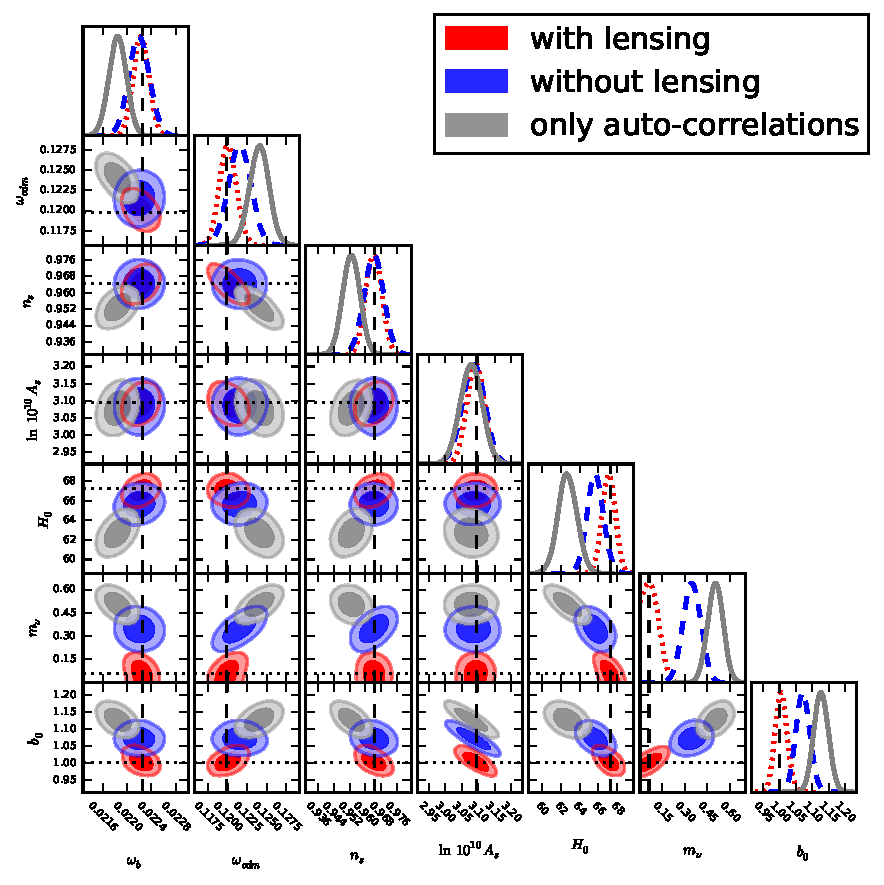
\includegraphics[width=\textwidth]{figures/chapter-mnu/triangle_figure_MCDM_bias_cmb_prior.pdf}
  \caption{Two- and 1-D posteriors for the cosmological parameters inferred using Planck priors. We show the full analysis including lensing (red dotted), an analysis neglecting lensing (blue dashed) and considering only auto-correlations (gray solid).
    The 68\% and 95\% confidence intervals are shown.
    Intersections between vertical and horizontal lines denote the fiducial cosmology.
   See Table \ref{Table:2} for numerical values of the statistical quantities.
  }
  \label{fig:mcmc-cmb-prior}
\end{figure}

\subsection{Significance of the lensing detection}

We can quantify the strength with which we detect the lensing signal in our setup with the help of Bayesian model probabilities, comparing the case with lensing to the case without lensing. To do this, we introduce formally an extended model $\MM_L$ with an additional `lensing amplitude' parameter $A_L$ that multiplies the lensing contribution in the model. For the `with lensing' model $\MM_1$ we then set $A_L = 1$, while the `without lensing' case $\MM_0$ corresponds to $A_L=0$. In this way the two models are nested within the extended model and we can use the Savage-Dickey density ratio (SDDR) method to derive model probabilities (see e.g.\ \cite{Trotta:2005ar} for an explanation of the SDDR, and section 3 of \cite{Dirian:2016puz} for a more detailed description of the same reasoning as the one used here): with the SDDR, the Bayes factor $B$ between the case with fixed $A_L$ and the general case is given by the posterior for $A_L$ (marginalised over all other parameters) of the general model divided by prior, both taken at the nested point,
\begin{equation}
B_x \equiv \frac{P(D|\MM_x)}{P(D|\MM_L)} = \frac{P(A_L=x|D,\MM_L)}{P(A_L=x|\MM_L)} \, .
\end{equation}
Here $P$ denote probabilities, $D$ the data and $x$ is either 0 or 1.
%$\theta$ the other parameters in the model.
The Bayes factor between two models with given fixed values for $A_L$ is then simply the ratio of the Bayes factors relative to the extend model,
\begin{eqnarray}
B_{xy} &\equiv& \frac{P(D|\MM_x)}{P(D|\MM_y)} \nonumber \\
&=& \frac{P(D|\MM_x)}{P(D|\MM_L)} \frac{P(D|\MM_L)}{P(D|\MM_y)} = \frac{B_x}{B_y} \nonumber \\
 &=& \frac{P(A_L=x|D,\MM_L)}{P(A_L=y|D,\MM_L)} \, ,
\end{eqnarray}
where the last equality holds if $P(A_L=x|\MM_L)=P(A_L=y|\MM_L)$, e.g.\ for an uniform prior in $A_L$, which is what we will use. We see that the only information needed to determine $B_{xy}$ is the relative value of the posterior at $A_L=x$ and at $A_L=y$, and this is approximately given by the $\chi^2$ difference between these cases. As by construction $A_L=1$ (the case where we include lensing consistently) has $\Delta\chi^2=0$, we find simply that $\ln B_{01} \approx -\Delta\chi^2_{\mathrm{no~lensing}}/2$. We find thus that $\ln B_{01} \approx -1000$ when using auto- and cross-correlations, and $\ln B_{01} \approx -90$ to $-115$ when only taking into account autocorrelations. Both Bayes factors are way out on the often-used Jeffreys' scale \cite{Jeffreys:1939xee} where anything larger than 5 is considered as strong. In other words, lensing is detected in both cases with an overwhelming evidence.

We can also translate the $\Delta\chi^2$ value into an order-of-magnitude estimate of `the number of sigmas' with which we detect the lensing signal in our setup. Assuming a Gaussian probability distribution function for $A_L$ so that $\Delta\chi^2 \approx (A_L-1)^2/\sigma[A_L]^2$, we find that $\sigma[A_L]$ needs to be 0.022 in order to explain the observed $\Delta\chi^2$ values of 2064 and 2082. This implies that the lensing is measured roughly at the $45\sigma$  level. Lensing is clearly a strong signal in the photo-$z$ type survey that we have considered here. As also discussed above, most of the lensing signal is contained in the off-diagonal spectra. The $\Delta\chi^2$ values of 180 and 230 when only looking at the auto-correlations correspond to about $13\sigma$ to $15\sigma$, roughly comparable to the strength of the lensing detection in the {\it Planck} temperature power spectrum \cite{Ade:2015xua}.
%While it would be better for an accurate determination of the detection strength to include $A_L$ explicitly as a parameter in the MCMC, our discussion here provides at least an estimate of the strength of the signal.


This also confirms the result of~\cite{Montanari:2015rga}, which found that the lensing amplitude $A_L$ can be determined to an accuracy of the order of (1-2)\%  with a Euclid like photometric survey, with the constraints coming especially from the off-diagonal (inter-bin) correlations.


\section{Conclusions}
\label{chapter-mnu:conclusions}

In this paper we have shown that neglecting  lensing convergence leads to large shifts in the best fit values of cosmological parameters for the data sets
available from future surveys. As in the CMB, where the lensing of the power spectra is detected at over $10\sigma$ \cite{Ade:2015xua},
it will become mandatory to include lensing also in the analysis of galaxy surveys.

In the case studied here we have seen mainly an increase in the neutrino mass $m_\nu$ and a decrease in the spectral index $n_s$ when neglecting lensing. Also the product $A_sb_0^2$ which determines the amplitude of fluctuations increases. This comes from the fact that the magnification bias for the Euclid specifications is relatively large~\cite{Montanari:2015rga} (see also Appendix~\ref{apa}), so that the  density-lensing correlation in bins with $z>1$ contributes with a positive sign. At smaller redshifts which mainly measure correlations on smaller scales this has to be corrected since there the total lensing term $\propto (5s-2)\kappa$ contributes negatively. This can be achieved by lowering $n_s$ and increasing the neutrino mass.

We note that
the specific shifts which we have obtained in our analysis depend  on the details of the survey. The main, generic result is that in order to estimate cosmological parameters reliably with future galaxy surveys, we have to correctly include lensing with the measured magnification bias function, $s(z)$, defined by
$$ s(z)  \equiv \frac{\partial\log_{10} N(z,m<m_*)}{\partial m_*}\,,  $$
where $m_*$ is the limiting magnitude of the survey and $N(z,m)$ is the galaxy luminosity function of the survey at redshift $z$.

The fact that deep galaxy surveys are so sensitive to lensing, however, is not only a curse but also a blessing. It means that these surveys will allow us to determine a map of the lensing potential at different redshifts, i.e.\ perform `lensing tomography' with galaxy clustering. This will be a very interesting alternative to lensing tomography with shear measurements proposed, e.g.\
in~\cite{Heavens:2003jx}. Both techniques are challenging but they have different systematic errors and allow valuable cross-checks. So clearly both paths should be pursued.


\chapter{Determining $H_0$ with Bayesian hyper-parameters}
\label{chapter-h0}

\section{Introduction}
\label{chapter-h0:introduction}

Pinning down the Hubble constant $H_0$ is crucial for the understanding of the standard model of cosmology. It sets the scale for all cosmological times and distances and it allows to tackle cosmological parameters, breaking degeneracies among them (e.g., the equation of state for dark energy and the mass of neutrinos). The expansion rate of the universe can either be directly measured or inferred for a given cosmological model through cosmological probes such as the cosmic microwave background (CMB). Although accurate direct measurements of the Hubble constant have proven to be difficult (e.g., control of systematic errors, relatively small data sets, fully consistency of different methods for measuring distances), significant progress has been achieved  
over the past decades \cite{Freedman1996,Freedman:2010xv}. The \textit{Hubble Space Telescope (HST)} Key Project made possible to measure $H_0$ with an accuracy of $10\%$ by significantly improving the control of systematic errors \cite{Freedman2001}.  More recently, in the \textit{HST} Cycle $15$, the \textit{Supernovae and $H_0$ for the Equation of State (SHOES)} project has reported measurements of $H_0$ accurate to $4.7\%$ ($74.2 \pm 3.6 \, \km\, \second^{-1}\, \Mpc^{-1}$) \cite{Riess:2009pu}, then to $3.3\%$ ($73.8 \pm 2.4 \, \km\, \second^{-1}\, \Mpc^{-1}$) \cite{Riess:2011yx} and very recently to $2.4\%$ ($73.24 \pm 1.74 \, \km\, \second^{-1}\, \Mpc^{-1}$) \cite{Riess:2016jrr}. This remarkable progress has been achieved thanks to both an enlarged sample of SN Ia having a Cepheid calibrated distance, a reduction in the systematic uncertainty of the maser distance to $\NGC$, an increase of infrared observations of Cepheid variables in the Large Magellanic Cloud (LMC).  

The 2015 release in temperature, polarization and lensing measurements of the CMB by the \textit{Planck} satellite leads to a present expansion rate of the universe given by $H_0 = 67.81 \pm 0.92 \, \km \, \second^{-1}\, \Mpc^{-1}$ for the base six-parameter $\Lambda$CDM model \cite{Ade:2015xua}. As it is known, the derived estimation of $H_0$ from CMB experiments provide indirect and highly model-dependent values of the current expansion rate of the universe (requiring e.g., assumptions about the nature of dark energy, properties of neutrinos, theory of gravity) and therefore do not substitute a direct measurement in the local universe. Moreover, indirect determinations (in a Bayesian approach) rely on prior probability distributions for the cosmological parameters which might have an impact on the results.

The \textit{Planck} Collaboration used a `conservative' prior on the Hubble constant ($H_0=70.6\pm3.3\, \km\, \second^{-1}\, \Mpc^{-1}$) derived from a reanalysis of the Cepheid data used in \cite{Riess:2011yx}, done by G. Efstathiou in \cite{Efstathiou:2013via}: in this reanalysis, a different rejection algorithm was used (with respect to that in \cite{Riess:2011yx}) for outliers in the Cepheid period-luminosity relation (the so-called Leavitt Law); in addition, \cite{Efstathiou:2013via} used the revised geometric maser distance to $\NGC$ of \cite{Humphreys:2013eja}. Although consistent with the \textit{Planck} TT estimate at the $1\, \sigma$ level, this determination of $H_0$ assumes that there is no metallicity dependence in the Leavitt Law. Furthermore, it discards data (i) from both Large Magellanic Cloud (LMC) and Milky Way (MW) Cepheid variables (ii) from the sample of Cepheid variables in \cite{Riess:2011yx} using an upper period cut of $60$ days.\footnote{In \cite{Efstathiou:2013via} G. Efstathiou also shows results utilizing the rejection algorithm for outliers used in \cite{Riess:2011yx}, but with the revised geometric maser distance to $\NGC$ \cite{Humphreys:2013eja} which is about $4\%$ higher than that adopted by \cite{Riess:2011yx} in their analysis. Note that in \cite{Riess:2011yx} (see their page 13) the authors provided a recalibration of $H_0$ for each increase of $1\%$ in the distance to $\NGC$ : according to this recalibration and the revised geometric maser distance their measurement would be driven downwards from $H_0 = 74.8\, \km \, \second^{-1}\, \Mpc^{-1}$ to $H_0 \approx 73.8 \, \km \, \second^{-1}\, \Mpc^{-1}$ which is higher than all the reported values in table A1 of \cite{Efstathiou:2013via} for the R11 rejection algorithm.}

As discussed in \cite{Freedman:2010xv}, the sensitivity to metallicity of the Leavitt Law is still an open question. In fact, due to changes in the atmospheric metal abundance, a metallicity dependence in the Cepheid period-luminosity is expected. Discarding data involves somehow arbitrary choices (e.g., chauvenet's criterion, period cut, threshold T in \cite{Efstathiou:2013via}) and might hinder our understanding of the physical basis behind the incompatibility of data sets (if any) \cite{Press:1996fw}. Therefore, neither no metallicity dependence in Leavitt Law nor disregarding data seem to be very conservative assumptions. 

Once systematics are under control (like the presence of unmodeled systematic errors or biases in the outlier rejection algorithm for Cepheid variables), a reliable estimate of $H_0$ is very important also on theoretical grounds. Confirmation of significant discrepancies between direct and indirect estimates of $H_0$ would suggest evidence of new physics. Discrepancies could arise if the local gravitational potential at the position of the observer is not consistently taken into account when measuring the Hubble constant. Nevertheless, an unlikely fluctuation would be required to explain an offset as big as $2.4\,\sigma$ \cite{Marra2013a}. Second-order corrections to the background distance-redshift relation could bias estimations of the Hubble constant derived from CMB \cite{Clarkson:2014pda}. However, it was shown in \cite{Bonvin:2015uha} that those corrections are already taken into account in current CMB analyses.           

It is clear from \cite{Efstathiou:2013via} that the statistical analysis done when measuring $H_0$ plays a part in the final result (for instance, through the outlier rejection algorithm, data sets included, anchors distances included, the period cut on the sample of Cepheid variables, the prior on the parameters of the Period-Luminosity relation). Given the relevance of the Hubble constant for our understanding of the universe, it is necessary to confirm previous results and prove them robust against different statistical approaches.

The goal of this project is to determine the Hubble constant $H_0$ by using Bayesian hyper-parameters to reanalyse the Cepheid data set used in both \cite{Riess:2011yx} and \cite{Riess:2016jrr}. In Section \ref{chapter-h0:notation-and-method} we explain both our notation and the statistical method employed. We then apply the method to different data sets and determine $H_0$ in Section \ref{chapter-h0:Application}. We conclude and discuss our results in Section \ref{chapter-h0:Summary}. 

\section{Notation and formalism}
\label{chapter-h0:notation-and-method}

\subsection{Distances and standard candles}

Astrophysical objects with a known luminosity -- the so-called standard candles-- are used to probe the expansion rate of the universe. In particular, measuring redshifts and apparent luminosities for supernovae type Ia (SNe Ia) one can establish an empirical redshift-distance relation for these objects. In order to estimate distances to SNe Ia one uses the luminosity distance
\begin{equation}
d_L \equiv \left(\frac{L}{4\pi l} \right)^{1/2} \, , \label{Eq:luminosity-distance-obs}
\end{equation}
where $L$ and $l$ are the absolute luminosity and the apparent luminosity, respectively. For historical reasons the apparent bolometric luminosity $l$ is defined so that 
\begin{equation}\label{Eq:apparent-luminosity}
l = 10^{-2m/5}\times 2.52 \times 10^{-5}\, \mathrm{erg/ cm^2}\, \second
\end{equation}
where $m$ is the apparent bolometric magnitude \cite{Weinberg:1972kfs}. Similarly, one can define the absolute bolometric magnitude $M$ as the apparent bolometric magnitude a source would have at a distance 10 $\mathrm{pc}$
\begin{equation}\label{Eq:absolute-luminosity}
L = 10^{-2M/5} \times 3.02 \times 10^{35}\, \mathrm{erg/}\second.
\end{equation}
Combining equations \eqref{Eq:luminosity-distance-obs}-\eqref{Eq:absolute-luminosity} it is possible to express the luminosity distance in terms of the distance modulus $m-M$:
\begin{equation}
\mu_0 \equiv m - M = 5 \log_{10} \left(\frac{d_L}{1 \mathrm{Mpc}} \right) + 25 \, . \label{Eq:distance-modulus}
\end{equation}

One can also estimate the luminosity distance $d_L$ of a light source with redshift $z$ within the context of General Relativity. Assuming a flat FLRW metric, one can compute the luminosity distance  
\begin{equation}\label{Eq:luminosity-distance-the}
d_L(z) = (1+z) c \int_0^z \frac{dz'}{H(z')} \, 
\end{equation}
where $c$ is the speed of light and $H(z)$ is the Hubble function. Since nowadays the empirical curve for $d_L(z)$ is reasonably well known for relatively small redshift, the Hubble function may then be usefully expressed as a power series in Eq. \eqref{Eq:luminosity-distance-the} leading to
\begin{equation}\label{Eq:luminosity-distance-the-small-z}
d_L(z) \equiv \frac{cz}{H_0}  ( 1+\delta(z)) \approx \frac{cz}{H_0} \left\{ 1 + \frac{1}{2} [1-q_0] z - \frac{1}{6} [1-q_0 - 3 q_0^2 + j_0] z^2 + O(z^3) \right\}
\end{equation} 
where $H_0$ is the Hubble constant, $q_0$ is the present acceleration parameter, $j_0$ the present prior deceleration parameter, and $\delta(z)$ defines a function that vanishes as $z\rightarrow 0$ and can be approximately expressed as a series expansion in redshift starting with a term linear in $z$.

Having both an empirical curve and a theoretical estimation of $d_L(z)$ for a given set of astrophysical objects, we can then try to find the parameters which fit the data the best. Equating Eqs. \eqref{Eq:distance-modulus} and \eqref{Eq:luminosity-distance-the-small-z} we obtain that
\begin{equation}\label{Eq:av-definition}
5 \log_{10} ( c z ( 1+\delta(z) )) - m_X = 5 \log_{10} H_0 - M_X - 25 \equiv 5 a_X \, ,
\end{equation}
where $X$ denotes the use of wavelength band $X$ (e.g., $U$ for ultraviolet, $B$ for blue, and $V$ for visual) and $a_X$ is a constant which defines the intercept of the $\log_{10} cz - 0.2\, m_X$ relation. Defining $\delta(z)$ through $q_0 = -0.55$ and $j_0 = 1$ \cite{Riess:2006fw}, Riess et al. \cite{Riess:2011yx} used the $V$ wavelength band Hubble diagram for 153 nearby SN-Ia in the red shift range $0.023 < z < 0.1$ (a conservative lower limit in red shift imposed to avoid the possibility of a local, coherent flow biasing the results)
to measure the intercept $a_V = 0.697 \pm 0.00201$. Using the Hubble diagram for $217$ $\SNe$ in the red shift range $0.023 < z < 0.15$, Riess et al. \cite{Riess:2016jrr} found $a_B = 0.71273 \pm 0.00176$.

From Eqs. \eqref{Eq:distance-modulus} and \eqref{Eq:av-definition} one can easily express the apparent magnitude $m_X^{\SNe}$ of a SNe Ia in terms of its distance modulus $\mu_0$, the Hubble constant $H_0$, and the intercept $a_X$ as
\begin{equation}
m_X^{\SNe} =  5 \log_{10} H_0 + \mu_0 - 5 a_X - 25 \, . \label{Eq:apparent-magnitude-H0}
\end{equation}
At this point (having measured $a_X$) we are again in a position where we can try to find the parameters $H_0$ and $\mu_0$ which adjust the best the observed $m^{\SNe}_X$. Cepheid variables -- another type of standard candle -- are stars whose apparent luminosity is observed to vary more or less regularly with time. There exist a few known galaxies ($19$ up to date \cite{Riess:2016jrr}) which simultaneously host both SNe Ia and Cepheid variables, thus providing the means to measure the distance parameter $\mu_{0,i}$ for the $i\mathrm{th}$ SN Ia through the Leavitt Law \cite{1912HarCi.173....1L}. According to the Leavitt Law there is a relation between period and luminosity of Cepheids: in the $i\mathrm{th}$ galaxy, the pulsation equation for the $j\mathrm{th}$ Cepheid star with apparent magnitude $m^{\Cepheid}_{X,i,j}$ (in the passband $X$) and period $P_{i,j}$ leads to a relation 
\begin{equation}\label{Eq:P-L-equation}
m^{\Cepheid}_{X,i,j} = \mu_{0,i} + M^{\Cepheid}_X + b_X (\log P_{i,j}-1) + Z_X \Delta \log[O/H]_{i,j},
\end{equation}
where $Z_X$ is the metallicity parameter, $b_X$ is the slope of the period-luminosity relation, and $M^{\Cepheid}_X$ is the Cepheid zero point. In principle, a simultaneous fit of Eqs. \eqref{Eq:apparent-magnitude-H0} and \eqref{Eq:P-L-equation} to observed $\SNe$ and Cepheid variables magnitudes would provide constraints for the expansion rate of the universe. 

Constraints for the parameters of the period-luminosity relation \eqref{Eq:P-L-equation} can be improved by adding galaxies containing Cepheid stars and for which a direct measurement of their distance (or the derived distance modulus $\mu_0$) is known. This is the case for the megamaser system $\NGC$, LMC, and M31. Although the sample of MW Cepheid variables with parallax measurements is relatively small ($15$ up to date \cite{Riess:2016jrr}) and mostly dominated by Cepheid stars with period $P<10$ days, their inclusion helps to further constrain parameters in the period-luminosity relation. Therefore, the inclusion of any of these anchor distances in a simultaneous fit to Eqs. \eqref{Eq:apparent-magnitude-H0}-\eqref{Eq:P-L-equation} helps to improve constraints on the distance parameters $\mu_{0,i}$ for the SNe Ia hosts and hence the Hubble constant $H_0$. 

\subsection{Hyper-parameters}

Astrophysical observations are difficult, and it is not easy to estimate and include the associated errors and uncertainties correctly. Often the data sets show outliers with error bars that are much smaller than the standard deviation from the expected fit, for reasons that are not well understood or difficult to quantify. An analysis needs to deal with such outliers, typically by removing them based on some rejection rule.
As discussed in \cite{Riess:2009pu,Riess:2011yx,Efstathiou:2013via}, the rejection of outliers on the Cepheid period-luminosity relation has a non-negligible effect on the determination of the expansion rate of the universe. One can argue that an outlier rejection criterion: i) involves arbitrary choices (e.g., Chauvenet's criterion, period cut) which might bias the results ii) rejects data, thus increasing error bars and hindering a better understanding of the data sets \cite{Press:1996fw}. The hyper-parameters (HPs, hereafter) method offers a Bayesian alternative to {\em{ad hoc}} selection of data points, avoiding problems associated with using incompatible data points \cite{Lahav:1999hu}. Instead of adopting an a priori rejection criterion  (galaxy-by-galaxy basis as in \cite{Riess:2009pu,Riess:2011yx} or from a global fit as in \cite{Efstathiou:2013via}), in this work we analyse {\em all} the available measurements with Bayesian HPs. The latter effectively allow for relative weights in the Cepheid variables, determined on the basis of how good their simultaneous fit to the model is. 

HPs allow to check for unrecognised systematic effects by introducing a rescaling of the error bar of data point $i$, $\sigma_i \rightarrow \sigma_i/\sqrt{\alpha_i}$. Here $\alpha_i$ is a HP associated with the data point $i$ \cite{Lahav:1999hu}.
In order to explain how HPs work, we start by assuming a Gaussian likelihood for the datum $D_i$,
\begin{equation}\label{Eq:Gaussian-likelihood}
P_G(D_i|\vec{w}) = \tilde{N}_i \, \frac{\exp(-\chi^2_i(\vec{w})/2)}{\sqrt{2\pi}},
\end{equation}
where $\chi^2_i$ and the normalisation constant $\tilde{N}_i$ are given by
\begin{equation}\label{Eq:chi2} %\label{Eq:normalization-Gaussian-likelihood}
\chi^2_i \equiv \frac{\left( x_{\obs,i} - x_{\pred,i}(\vec{w}) \right)^2}{\sigma_i^2} \, , \quad
\tilde{N}_i = 1/\sqrt{\sigma_i^2} \, .
\end{equation}
Here for each measurement $x_{\obs,i}$ there is a corresponding error $\sigma_i$ and a prediction $x_{\pred,i}(\vec{w})$, ($\vec{w}$ being the parameters of a given model). Suppose that some errors have been wrongly estimated due to unrecognised (or underestimated) systematic effects and use hyper-parameters  \cite{Lahav:1999hu} to control the relative weight of the data points in the likelihood. For each measurement {$i$} we introduce a HP to rescale $\sigma_i$ as mentioned above. In that case the Gaussian likelihood becomes \cite{Lahav:1999hu}
\begin{equation}\label{Eq:HP-Gaussian-likelihood}
P(D_i|\vec{w},\alpha_i) = \tilde{N}_i \, \alpha_i^{1/2}\, \frac{\exp(-\alpha_i \chi^2_i(\vec{w})/2)}{\sqrt{2\pi}}.
\end{equation}

However, in general we do not know what value of $\alpha_i$ is correct. In order to circumvent this problem, 
we follow a Bayesian approach, introducing the $\alpha_i$ as nuisance parameters and marginalising over them. Given a set of data points $ \lbrace D_i \rbrace$, we can write the probability for the parameters $\vec{w}$  as
\begin{equation}\label{Eq:probability-of-w}
P(\vec{w}|\lbrace D_i \rbrace) = \int \dots \int P(\vec{w},\lbrace \alpha_i \rbrace|\lbrace D_i \rbrace)\, d\alpha_1 \dots d\alpha_N,
\end{equation}
where $N$ is the total number of measurements. Bayes' theorem allows us to write 
\begin{equation}\label{Eq:probability-of-w-alphas-1}
P(\vec{w},\lbrace \alpha_i \rbrace|\lbrace D_i \rbrace) = \frac{P(\lbrace D_i \rbrace|\vec{w},\lbrace \alpha_i \rbrace)\, P(\vec{w},\lbrace \alpha_i \rbrace)}{P(D_1,\dots,D_N)}
\end{equation}
and 
\begin{equation}\label{Eq:probability-of-w-alphas-2}
P(\vec{w},\lbrace \alpha_i \rbrace) = P(\vec{w}|\lbrace \alpha_i \rbrace)\, P(\lbrace \alpha_i \rbrace).
\end{equation}
As in \cite{Lahav:1999hu} we assume:
\begin{subequations}\label{Eq:assumptions}
\begin{align}
\label{Eq:assumptions:1}
P(\lbrace D_i \rbrace|\vec{w},\lbrace \alpha_i \rbrace) & = P(D_1|\vec{w},\alpha_1)\dots P(D_N|\vec{w},\alpha_N),
\\
\label{Eq:assumptions:2}
P(\vec{w}|\lbrace \alpha_i\rbrace) & = \mathrm{constant},
\\
\label{Eq:assumptions:3}
P(\lbrace \alpha_i \rbrace) & = P(\alpha_1)\dots P(\alpha_N).
\end{align}
\end{subequations}

Thus far the formalism is fairly general and it contains two unspecified functions: probability distributions for both data points and HPs. In this work we will assume uniform priors for HPs ($P(\alpha_i)=1$) and that errors never become smaller than their reported value ($\alpha_i \in [0,1]$).\footnote{We have examined the more general case of an improper Jeffrey's prior (allowing decreasing as well as increasing error bars). This works well when many data points are associated to the same HP so that the $\chi^2$ never vanishes. But when each data point has its own associated HP then the model curve can pass through that data point so that $\chi^2_i=0$. In this case the likelihood grows without bounds as $\alpha_i\rightarrow 0$, in other words the HP-marginalised likelihood is singular when at least one of the points has $\chi^2=0$ as can also be seen from Eq. (16) in \cite{Lahav:1999hu}.} A low posterior value of the HP indicates that the point has less weight within the fit. This may indicate the presence of systematic effects or the requirement for better modelling. With these assumptions Eq.~\eqref{Eq:probability-of-w} now becomes:

\begin{equation}\label{Eq:probability-of-w-2}
P(\vec{w},\lbrace D_i \rbrace) = \frac{P(D_1|\vec{w})\dots P(D_N|\vec{w})}{P(D_1,\dots,D_N)},
\end{equation}
where 
\begin{equation}\label{Eq:probability-of-w-2b}
P(D_i|\vec{w}) \equiv \int_0^1 P(D_i|\vec{w},\alpha_i)\, d\alpha_i.
\end{equation}

The integral in Eq. \eqref{Eq:probability-of-w-2b} can be explicitly evaluated for the Gaussian HP likelihood (\ref{Eq:HP-Gaussian-likelihood}), it gives, for each data point,
\begin{eqnarray}\label{Eq:hyper-likelihood}
P(D_i|\vec{w}\,) = \tilde{N}_i \, \left(\frac{ \mathrm{Erf}\left( \frac{\chi_i(\vec{w})}{\sqrt{2}} \right)  -\sqrt{\frac{2}\pi} \chi_i(\vec{w}) \exp(-\chi^2_i(\vec{w})/2)}{ \chi^3_i(\vec{w})} \right).
\end{eqnarray}
We can now rewrite Eq. \eqref{Eq:probability-of-w-2} as
\begin{equation}\label{Eq:probability-of-w-2c}
\ln P(\vec{w},\lbrace D_i \rbrace) = \sum_i \ln \tilde{N}_i + \ln \tilde{\chi}^2_i, 
\end{equation} 
where constant terms have been omitted and where
\begin{equation}\label{Eq:hyper-chi2}
\tilde{\chi}^2_i(\chi^2_i(\vec{w})) \equiv \frac{ \mathrm{Erf}\left( \frac{\chi_i(\vec{w})}{\sqrt{2}} \right)  -\sqrt{\frac{2}\pi} \chi_i(\vec{w}) \exp(-\chi^2_i(\vec{w})/2)}{ \chi^3_i(\vec{w})}.
\end{equation}

One can easily obtain the most likely value for each HP by maximizing \eqref{Eq:HP-Gaussian-likelihood} w.r.t HPs at a given set of best fit parameters $\vec{w}$. We find that for each data point the effective HP is given by:
\begin{subequations}\label{Eq:effective-HPs}
\begin{align}
\label{Eq:effective-HP-1}
\alpha^{\eff}_i & = 1,\quad \mathrm{if} \quad \chi^2_i\leq1
\\
\label{Eq:effective-HP-2}
\alpha^{\eff}_i & = \frac{1}{\chi^2_i},\quad \mathrm{if} \quad \chi^2_i> 1.
\end{align}
\end{subequations}
We will now apply HPs to combine Cepheid variable measurements and determine the current expansion rate of the universe. We explore the parameter space $\vec{w}$ with the help of a Markov Chain Monte Carlo (MCMC) approach using flat priors if not specified differently.

\begin{figure}[hbtp]
\centering
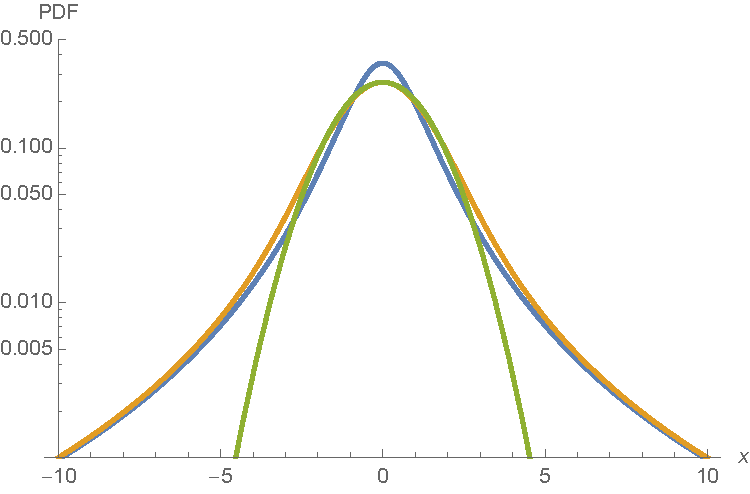
\includegraphics[width=\textwidth]{figures/chapter-h0/hyperparam_like.pdf}
\caption{The hyper-parameter-marginalized probability distribution function (pdf) of Eq.\ (\ref{Eq:hyper-likelihood}) in yellow. Close to the origin, $x=0$, it is similar to a Gaussian pdf with $\sigma = (5/2)^{1/3}$ (green), except that its amplitude at the peak is 10.5\% lower than a normalised Gaussian. Asymptotically for $|x|\rightarrow\infty$ it decreases as $1/x^3$ and looks like a student's t distribution with 2 degrees of freedom (blue), but the latter is narrower at small $x$.}
\end{figure}

\section{Applying hyper-parameters}
\label{chapter-h0:Application}

In this section we will apply HPs to determine the Hubble constant. First, we will illustrate how the method works by fitting the period-luminosity relation of Cepheid variables in the LMC, the MW, and the megamaser system $\NGC$. This will allow us to compare with results in \cite{Efstathiou:2013via}. Then, in Subsection \ref{Subsection:combining-anchors} we determine $H_0$ with the Cepheid sample and SNe hosts in \cite{Riess:2011yx} (hereafter, R11). When this work was about to finish a new enlarged and improved sample of Cepheid variables and SNe hosts came out \cite{Riess:2016jrr} (hereafter, R16); we determine the expansion rate of the universe with this data set in Subsection \ref{Subsection:combining-anchors-R16}.  

\subsection{The LMC Cepheid variables}
\label{Subsection:LMC}

We start out our analysis by applying HPs to the set of 
53 LMC Cepheid variables with $H$-band magnitudes, $m_H$, listed in Table 3 of  \cite{2004AJ:128.2239P} and $V$, $I$ band magnitudes, $m_V$, $m_I$, listed in Table 4 of \cite{2002ApJS:142:71S}. Following \cite{Riess:2016jrr}, we rely primarily on (near-infrared) NIR `Wesenheit reddening-free' magnitudes, defined as 
\begin{equation}\label{Eq:Wesenheit-reddening-free}
m_{W,i} = m_{H,i} - R\, (m_{V,i} - m_{I,i}),
\end{equation}
where $R$ is a constant defining the reddening law; in Subsections \ref{Subsection:LMC}--\ref{Subsection:combining-anchors}, where R11 data set is used, we set $R=0.410$ as G. Efstathiou did \cite{Efstathiou:2013via}; when utilising R16 data set, we analyse the sensitivity of $H_0$ to variations in $R$. For the purpose of comparing with \cite{Efstathiou:2013via} we neglect for now metallicity dependence and fit the data with a period-luminosity relation
\begin{equation}\label{Eq:P-L-LMC}
m^P_W = A + b_W (\log P - 1),
\end{equation}
where $A = \mu_{0,\LMC} + M_W$ in notation of Eq. \eqref{Eq:P-L-equation} and $P$ is the period.\footnote{We have dropped the label `$\Cepheid$' in the magnitudes for sake of simplicity.} In order to apply HPs we define 
\begin{equation}\label{Eq:chi2-LMC}
\chi^{2,\LMC}_{i} = \frac{(m_{W,i} - m^P_{W})^2}{\sigma_i^2 + \sigma^{2,\LMC}_{\intt}},
\end{equation}
where $\sigma_i$ is the observational error on $m_{W,i}$ and $\sigma_{\intt}^{\LMC}$ is what is referred to as `internal scatter' in \cite{Efstathiou:2013via}. The internal scatter is a common additional dispersion of the data points that is independent of the measurement error and due to variations in the physical mechanism behind the period-luminosity relation. As we do not know the origin and magnitude of the internal scatter precisely, we add it as an additional random variable and marginalise over it.\footnote{Note that in R16 data set this intrinsic dispersion is already included in the total statistical uncertainty reported in their table 4 \cite{Riess:2016jrr}. Consequently, when analysing the R16 data set we do not include an additional $\sigma_{\intt}$.} More precisely, we sample in $\log \sigma_{\intt}$ with a flat prior $\ln \sigma_{\intt} \in [-3,-0.7]$.
Maximizing  
\begin{equation}
\label{Eq:likelihood-HP-LMC}
\ln P^{\LMC}(A,b_W,\lbrace D_i \rbrace) = \sum_{i} \ln \tilde{\chi}_i^{2}(\chi^{2,\LMC}_{i}) + \ln \tilde{N}^{\LMC}_{i},
\end{equation}
where 
\begin{equation}
\label{Eq:normalization-LMC}
\tilde{N}^{\LMC}_i = \frac{1}{\sqrt{\sigma_i^2 +\sigma^{2,\LMC}_{\intt}}},
\end{equation}
we find the best-fitting parameters of the period-luminosity relation \eqref{Eq:P-L-LMC}. Table \ref{Table:LMC-fits} shows results for different period cuts. Figure \ref{Fig:LMC-Cepheid-variables-fit-c} shows the period-luminosity relation for the LMC Cepheid variables and the best fit of cases (c) and (d) in Table \ref{Table:LMC-fits}. We also show in Figure.\ \ref{fig:sigmaint} the posterior probability distribution function (pdf) of $\sigma_{\intt}$ for the fits (c) and (d) of Table \ref{Table:LMC-fits}.

\begin{table}[tbp]
\centering
\begin{tabular}{@{}ccccc}
\hline
\multicolumn{5}{c}{LMC Cepheid variables} \\
\hline
Fit & $A$ & $b_W$ & $\sigma_{\intt}^{\LMC}$ & Period cut \\
\hline
 a & $12.570\,(0.035)$ & $-3.32\,(0.10)$ & $0.06$ & $10<P<60$ \\
  
 b & $12.562\,(0.016)$&$-3.30\,(0.05)$ & $0.06$ & $P<60$ \\

 c & $12.562\,(0.016)$& $-3.31\,(0.05)$& $0.06$ & $P<205$ \\

 d & $12.555\,(0.019)$& $-3.24\,(0.06)$& $0.12$ & $P<205$ \\
\hline
\end{tabular}
\caption{\label{Table:LMC-fits} Mean value and standard deviation (in brackets) for the parameters in the period-luminosity relation. Fits (a), (b), and (c) use HPs whereas fit (d) is a standard $\chi^2$ minimization as done in \cite{Efstathiou:2013via}.}
\end{table}


\begin{figure}[tbp]
\centering % \begin{center}/\end{center} takes some additional vertical space
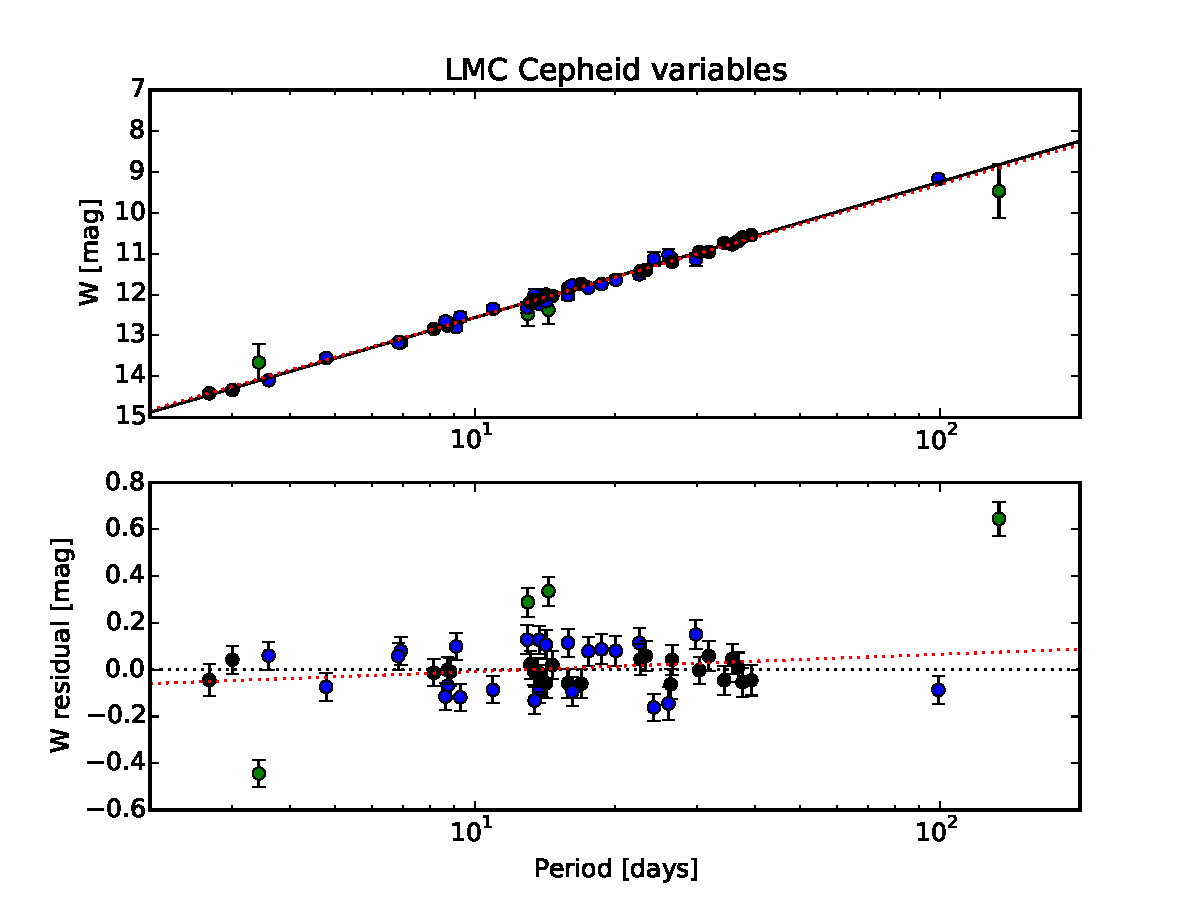
\includegraphics[width=\textwidth]{figures/chapter-h0/effective_HP_cepheids_LMC.pdf} 
\caption{Period-luminosity relation for the LMC Cepheid variables. The upper panel shows the best fit of both the case (c) (solid black line) and case (d) (red dotted line) in Table \ref{Table:LMC-fits}. Error bars have been rescaled with corresponding effective HPs which are colour-coded as follows: black if $\alpha_{\eff} = 1$, blue if $10^{-1}\leq \alpha_{\eff} < 1$, green if $10^{-2}\leq \alpha_{\eff} < 10^{-1}$, red if  $10^{-3} \leq \alpha_{\eff} < 10^{-2}$ and yellow if $\alpha_{\eff} < 10^{-3}$. Lower panel shows magnitude residuals; error bars are not rescaled and colours correspond to those in upper panel. The red dotted line in the lower panel shows the difference between the best fits in the upper panel.}
\label{Fig:LMC-Cepheid-variables-fit-c}
\end{figure}

\begin{figure}[hbtp]
\centering
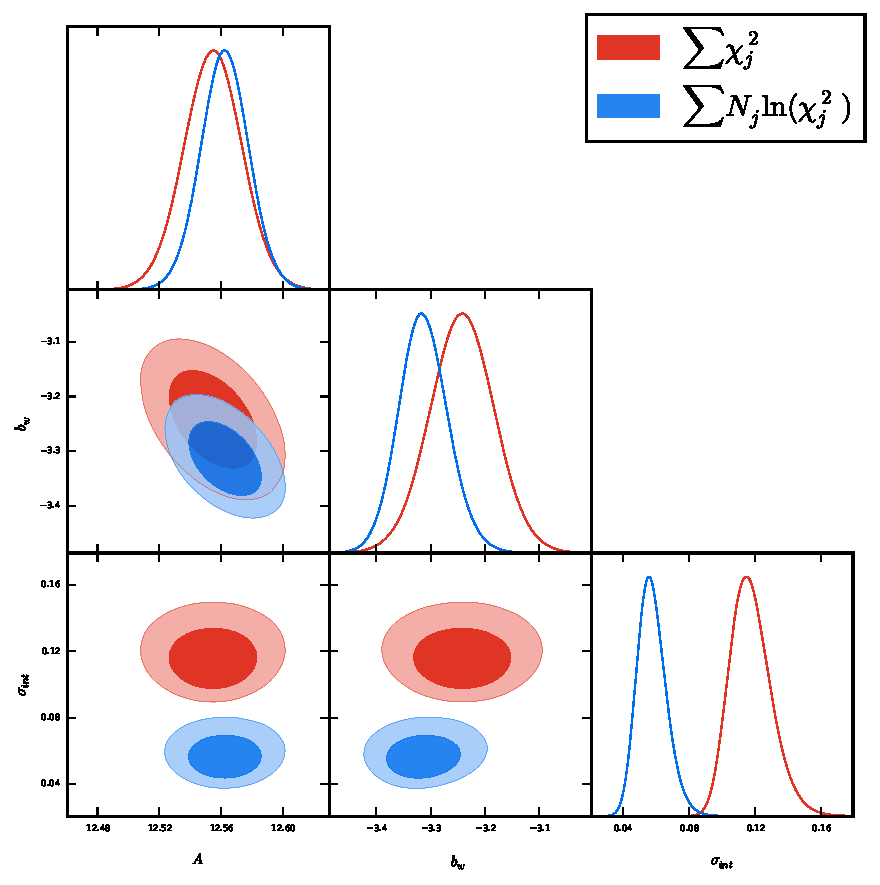
\includegraphics[width=\textwidth]{figures/chapter-h0/triangle_figure_joint_sigma_int.pdf}
\caption{Two- and 1D posteriors for the parameters in the period-luminosity relation. Red shows a standard $\chi^2$ minimisation and blue uses HPs.  }
\label{fig:sigmaint}
\end{figure}

The LMC Cepheids are also treated as illustrative example in section 2 of \cite{Efstathiou:2013via}. This allows us to compare the approach used there, which does not use hyper-parameters, with the results found here. In our approach, the posterior mean values of $A$ and $b_W$ always lie in between the values given in \cite{Efstathiou:2013via}. They do also not depend significantly on the period cut (except that the error becomes larger for the most restrictive cut, $10<P<60$. We conclude that our treatment performs reasonably well when compared to the standard $\chi^2$ approach, and also that the hyper-parameters allow to use all the available data without significant bias. We will investigate this conclusion further as we add more data.

In Figure \ref{Fig:LMC-Cepheid-variables-fit-c} we also show the colour-coded effective HP value for all the data points in the LMC Cepheid sample, based on (\ref{Eq:effective-HP-1}) and (\ref{Eq:effective-HP-2}). Especially the lower panel, where we plot the residuals with respect to the best fit, shows clearly how outliers have a lower effective hyper- parameter and thus less weight. If instead we used a standard $\chi^2$ fit to all of these points (i.e.\ without period cut) then the fit would be pulled towards a steeper slow (higher $b_W$) by the green points near the extrema of $P$ as shown by the red dotted line in the upper panel of Figure \ref{Fig:LMC-Cepheid-variables-fit-c}. 

The LMC distance modulus derived from observations of eclipsing binaries \cite{Pietrzynski:2013gia} is 
\begin{equation}
\mu_{0,\LMC}^{\obs} = 18.49 \pm 0.05\, \magn,
\label{Eq:LMC-measured-distance-modulus}
\end{equation}
that together with $A$ from Table \ref{Table:LMC-fits} for fit (c) gives a Cepheid zero point
\begin{equation}\label{Eq:zero-point-LMC}
M_W = -5.93 \pm 0.07\, \magn.
\end{equation}


\subsection{The MW Cepheid variables}
\label{Subsection:MW-1}

Next, we discuss the set of $13$ MW Cepheid stars with parallax measurements listed in Table 2 of \cite{vanLeeuwen:2007xw} (eliminating Polaris as in \cite{Efstathiou:2013via} and correcting for Lutz-Kelker bias). We consider the MW Cepheids separately here because, as we will see, the MW data pushes the inferred value of $H_0$ to higher values, and it is thus important to check whether there is a reason to discard this data set or not.

The period-luminosity relation for those Cepheid stars is given by
\begin{equation}\label{Eq:P-L-MW}
M^P_W = M_W + b_W (\log P - 1),
\end{equation}
where $Z_W=0$ in Eq. \eqref{Eq:P-L-equation}, $M^P_W = m^P_W - \mu_{\pi}$ and $\mu_\pi$ is the distance modulus derived from parallaxes. Here we define 
\begin{equation}\label{Eq:chi2-MW}
\chi^{2,\MW}_{i} = \frac{(M_{W,i} - M^P_{W})^2}{\sigma_i^2 + \sigma^{2,\MW}_{\intt}},
\end{equation}
where $\sigma_i$ is the observational error on $M_{W,i}$ and $\sigma_{\intt}^{\MW}$ is once more the internal dispersion (that we again include as a free, marginalised parameter as in the previous section on LMC Cepheids). Maximizing  
\begin{equation}
\label{Eq:likelihood-HP-MW}
\ln P^{\MW}(M_W,b_W,\lbrace D_i \rbrace) = \sum_{i} \ln \tilde{\chi}_i^{2}(\chi^{2,\MW}_{i}) + \ln \tilde{N}^{\MW}_{i},
\end{equation}
where 
\begin{equation}
\label{Eq:normalization-MW}
\tilde{N}^{\MW}_i = \frac{1}{\sqrt{\sigma_i^2 +\sigma^{2,\MW}_{\intt}}},
\end{equation}
we find the best-fitting parameters of the period-luminosity relation \eqref{Eq:P-L-MW}. They are 
\begin{equation}\label{Eq:MW-bestfit}
M_W = -5.88 \pm 0.07\,\magn  , \qquad b_W = -3.30 \pm 0.26  , \qquad \sigma_{\intt}^{\MW} = 0.02 ,
\end{equation}
in good agreement with fits in Table \ref{Table:LMC-fits} and with \cite{Efstathiou:2013via}. 
Figure \ref{Fig:MW-Cepheid-variables} shows the period-luminosity relation for the MW Cepheid variables and best fit in Eq. \eqref{Eq:MW-bestfit}.

\begin{figure}[tbp]
\centering % \begin{center}/\end{center} takes some additional vertical space
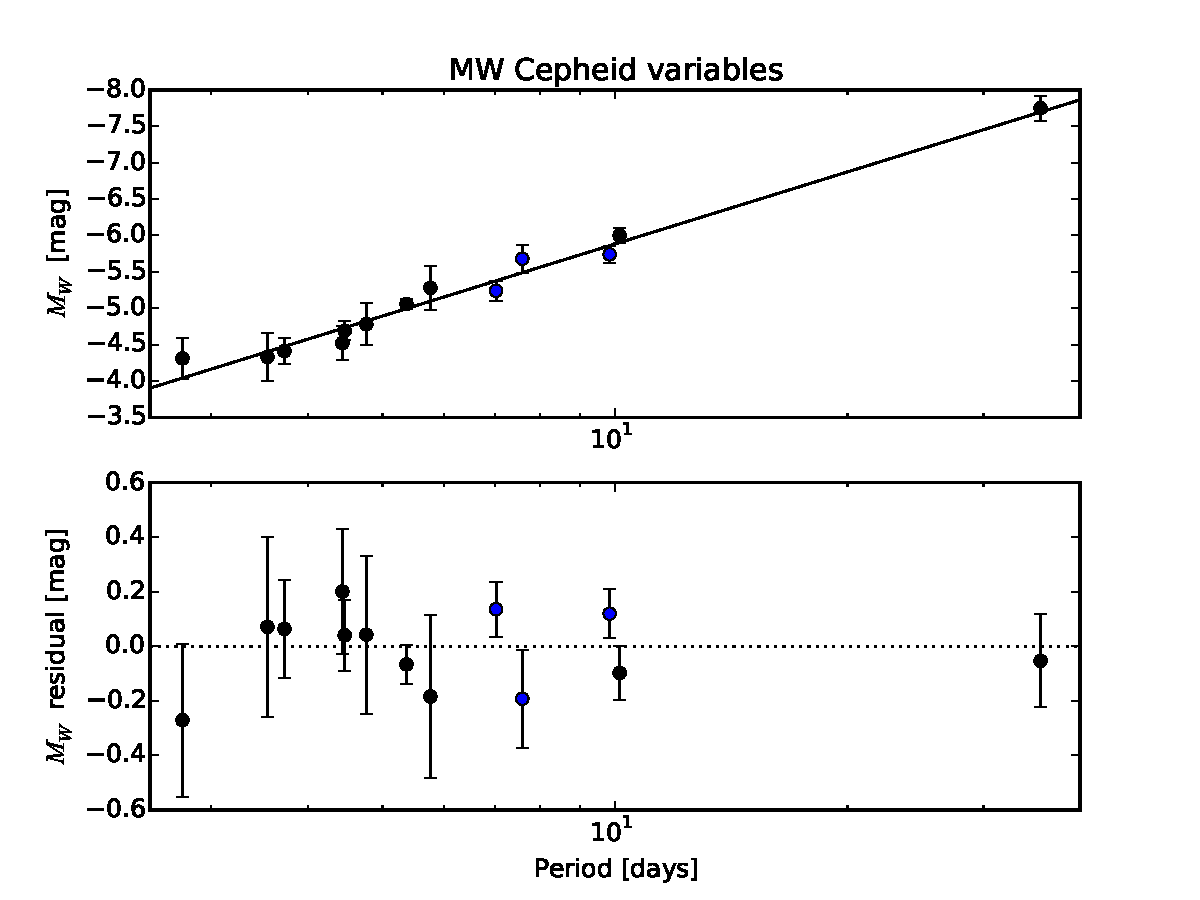
\includegraphics[width=\textwidth]{figures/chapter-h0/effective_HP_cepheids_MW.pdf} 
\caption{Period-luminosity relation for the MW Cepheid variables. Upper panel shows the best fit. Error bars have been rescaled with corresponding effective HPs which are colour-coded as in Figure \ref{Fig:LMC-Cepheid-variables-fit-c}. Lower panel shows magnitude residuals; error bars are not rescaled and colours correspond to those in upper panel.}
\label{Fig:MW-Cepheid-variables}
\end{figure}

The consistency in both the Cepheid zero point $M_W$ (see Eq. \eqref{Eq:zero-point-LMC}) and the slope $b_W$ between the MW and the LMC Cepheid data, as well as the lack of marked outliers visible in Figure\ \ref{Fig:MW-Cepheid-variables} provides no argument for excluding the MW data, at least based on the Cepheid stars. For this reason, we will include the MW data in our `standard analysis' discussed in Section \ref{Subsection:combining-anchors}. We also note that our tests have shown that the MW Cepheid data have no preference for a non-zero $\sigma^{\MW}_{\intt}$, although including it does not change the fit significantly.

\subsection{Cepheid variables in the megamaser system\\
 $\NGC$}
\label{Subsection:NGC4258}

In this subsection we use the set of $\NGC$ Cepheid variables included in the sample of \cite{Riess:2011yx} to fit the period-luminosity relation \eqref{Eq:P-L-LMC} setting now $A = \mu_{0, \NGC} + M_W$ and neglecting metallicity dependence. We find
\begin{figure}[tbp]
\centering % \begin{center}/\end{center} takes some additional vertical space
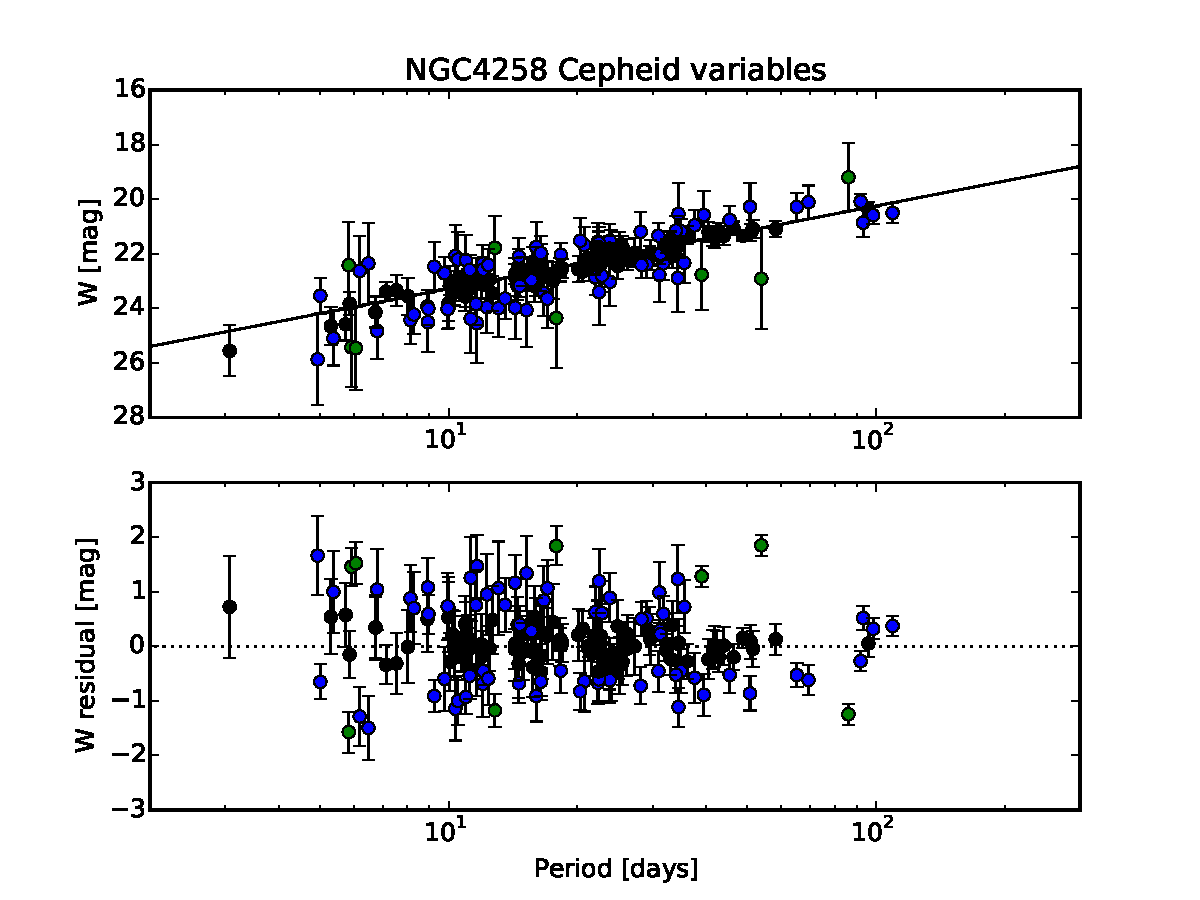
\includegraphics[width=\textwidth]{figures/chapter-h0/effective_HP_cepheids_NGC4258.pdf} 
\caption{Period-luminosity relation for the $\NGC$ Cepheid variables. Upper panel shows the best fit; error bars have been rescaled with corresponding effective HPs which are colour-coded as in Figure \ref{Fig:LMC-Cepheid-variables-fit-c}. Lower panel shows magnitude residuals; error bars are not rescaled and colours correspond to those in upper panel.}
\label{Fig:NGC4258-Cepheid-variables}
\end{figure}

\begin{equation}\label{Eq:NGC4258-bestfit}
A = 23.281 \pm 0.078\, \magn  , \qquad b_W = -3.02 \pm 0.17  , \qquad \sigma_{\intt}^{\NGC} = 0.12 .
\end{equation}
Figure \ref{Fig:NGC4258-Cepheid-variables} shows period-luminosity relation and residuals for the $\NGC$ Cepheid variables. Note that the slope $b_W$ for the fit \eqref{Eq:NGC4258-bestfit} is about $1.7\sigma$ away from the fit (c) in Table \ref{Table:LMC-fits} and the internal scatter $\sigma_{\intt}^{\NGC}=2\sigma_{\intt}^{\LMC}$. The $\NGC$ distance modulus derived from the geometric maser distance estimate to the active galaxy $\NGC$ \cite{Humphreys:2013eja} is 
\begin{equation}
\mu_{0,\NGC}^{\obs} = 29.40 \pm 0.07\, \magn,
\label{Eq:NGC4258-measured-distance-modulus-2013}
\end{equation}
which leads to a Cepheid zero point $M_W=-6.12 \pm 0.15\, \magn$, a value about $1.6\sigma$ away from that in Eq. \eqref{Eq:MW-bestfit}.\footnote{The standardised candle method for type IIP SNe \cite{Polshaw:2015ika} provides an alternative determination of the $\NGC$ distance modulus:
$\mu_{0,\NGC} = 29.25 \pm 0.26\, \magn$. Although compatible with \eqref{Eq:NGC4258-measured-distance-modulus-2013},  it is much less precise and therefore we do not include it in our analysis. }
In the next subsection we explore the possibility of whether or not a metallicity dependence in the period-luminosity relation may improve the agreement in both the Cepheid zero point $M_W$ and the slope $b_W$. 

\subsection{Metallicity dependence in the period-luminosity relation}\label{Subsection:Zw-dependence}

Although the Leavitt law is expected to depend at some level on the Cepheids metal abundance \cite{Freedman:2010xv}, thus far we have neglected this effect. Here we will study how an additional degree of freedom in the period-luminosity relation (i.e., $Z_W \neq 0$) impacts the fits we have presented. As in \cite{Efstathiou:2013via} we consider a mean metallicity $\Delta \log[O/H]=8.5$ for the LMC and $\Delta \log[O/H]=8.9$ for the MW. For all other galaxies we use the metallicity reported in Table 2 of \cite{Riess:2011yx}; Cepheid variables in those galaxies have a mean metallicity close to that of the Cepheid variables in the MW, $\Delta \log[O/H] \approx 8.9$.

Table \ref{Table:Zw-dependence-of-PL-relation} shows the fit for the period-luminosity relation \eqref{Eq:P-L-equation}  (setting $A=\mu_{0,i} + M_W$) for all the galaxies containing Cepheid variables. We notice that the effect of metallicity on both the slope $b_W$ and the Cepheid zero point $M_W$ (through its dependence on $A$) is never greater than $4.3\%$ (n3021) and $8.1\%$ (NGC4028), respectively. The metallicity parameter $Z_W$ is compatible with zero in all galaxies, its main effect being a small shift and a potentially large increase in the standard deviation of the Cepheid zero point due to a degeneracy between these two parameters (see Figure \ref{Fig:Main-analysis-fitM1a}). 

Another point worth noting from the results in Table \ref{Table:Zw-dependence-of-PL-relation} is the fact that the slope $b_W$ of about half of the host galaxies in the sample of \cite{Riess:2011yx} is less steep than the one of the LMC Cepheid variables, the shift being $\gtrsim 2\sigma$ for n4536, n4639, n1309, n4038, and n5584. This difference in the slope is however not improved by leaving more freedom in the metallicity dependence.

Cepheid zero point $M_W$ derived from MW Cepheids is insensitive to including metallicity dependence in the period-luminosity relation. For both LMC and $\NGC$ Cepheid variables, a small dependence on metallicity (strong prior) brings the Cepheid zero point in slightly better agreement with that derived from MW Cepheids. In particular, for the $\NGC$ distance modulus in Eq. \eqref{Eq:NGC4258-measured-distance-modulus-2013} and using a strong prior on $Z_W$, we obtain $M_W=-6.11 \pm 0.26$.

Because of the $M_W$-$Z_W$ degeneracy, and since the additional freedom in the metallicity dependence does not bring the different Cepheid data sets into better agreement,
we will use the `strong' prior on the metallicity, $Z_W = 0 \pm 0.02$, as our default choice.

\begin{table}[tbp]
\centering
\begin{tabular}{@{}ccccc}
\hline
\multicolumn{5}{c}{Sample of Cepheid variables} \\
\hline
galaxy & $A$ & $b_W$ & $Z_W$ & $\sigma_{\intt}$ \\
\hline
 LMC & $12.699\,(2.139)$ & $-3.31\,(0.05)$ & $-0.016\,(0.252)\,[W]$ & $0.06$ \\

LMC & $12.562\,(0.170)$ & $-3.31\,(0.05)$ & $0.000\,(0.020)\,[S]$ & $0.06$ \\
  
 MW & $-5.88\,(2.23)$ & $-3.30\,(0.26)$ & $0.000\,(0.250)\,[W]$ & $0.02$ \\

 MW & $-5.88\,(0.19)$ & $-3.30\,(0.26)$ & $0.000\,(0.020)\,[S]$ & $0.02$ \\
 
 $\NGC$ & $25.175\,(1.957)$ & $-3.00\,(0.17)$ & $-0.214\,(0.221)\,[W]$& $0.12$ \\

 $\NGC$ & $23.293\,(0.193)$ & $-3.02\,(0.17)$ & $-0.001\,(0.020)\,[S]$& $0.12$ \\
 
 n4536 & $24.620\,(1.866)$ & $-2.85\,(0.17)$ & $ 0.021\,(0.214)\,[W]$ & $0.07$ \\

 n4536 & $24.803\,(0.207)$ & $-2.84\,(0.17)$ & $ 0.000\,(0.020)\,[S]$ & $0.07$ \\
 
 n4639 & $26.572\,(1.846)$ & $-2.46\,(0.42)$ & $-0.147\,(0.210)\,[W]$ & $0.03$ \\
 
 n4639 & $25.303\,(0.302)$ & $-2.49\,(0.42)$ & $-0.001\,(0.020)\,[S]$ & $0.04$ \\
  
 n3982 & $26.591\,(1.724)$ & $-3.28\,(0.42)$ & $-0.083\,(0.200)\,[W]$ & $0.03$ \\
  
 n3982 & $25.888\,(0.283)$ & $-3.27\,(0.42)$ & $ 0.000\,(0.020)\,[S]$ & $0.03$ \\
   
 n3370 & $28.317\,(1.696)$ & $-2.99\,(0.20)$ & $-0.260\,(0.196)\,[W]$ & $0.02$ \\
 
 n3370 & $26.098\,(0.224)$ & $-3.03\,(0.20)$ & $-0.003\,(0.020)\,[S]$ & $0.02$ \\
  
 n3021 & $28.226\,(1.983)$ & $-2.86\,(0.51)$ & $-0.239\,(0.231)\,[W]$ & $0.03$ \\

 n3021 & $26.211\,(0.325)$ & $-2.99\,(0.50)$ & $-0.002\,(0.020)\,[S]$ & $0.03$ \\
  
 n1309 & $26.788\,(2.032)$ & $-2.09\,(0.42)$ & $-0.105\,(0.225)\,[W]$ & $0.03$ \\

 n1309 & $25.857\,(0.354)$ & $-2.08\,(0.42)$ & $-0.000\,(0.020)\,[S]$ & $0.03$ \\
   
 n4038 & $24.200\,(2.171)$ & $-2.47\,(0.27)$ & $0.092\,(0.243)\,[W]$ & $0.03$ \\

 n4038 & $25.011\,(0.291)$ & $-2.45\,(0.27)$ & $0.000\,(0.020)\,[S]$ & $0.03$ \\
    
 n5584 & $25.428\,(1.782)$ & $-2.83\,(0.24)$ & $0.013\,(0.204)\,[W]$ & $0.03$ \\   

 n5584 & $25.541\,(0.240)$ & $-2.83\,(0.24)$ & $0.000\,(0.020)\,[S]$ & $0.03$ \\   
 
\hline
\end{tabular}
\caption{\label{Table:Zw-dependence-of-PL-relation} Mean values and standard deviation (in brackets) in the period-luminosity relation parameters for the sample of Cepheid variables used in this work. The period range used to fit the data is the same used in fit (c) of Table \ref{Table:LMC-fits} ($P<205$ days). $[W]$ stands for a Gaussian prior with mean  $\bar{Z_W}=0$ and standard deviation $\sigma_{Z_W}=0.25$. $[S]$ stands for a Gaussian prior with $\bar{Z_W}=0$ and $\sigma_{Z_W}=0.02$. The internal dispersion for each galaxy is shown in the last column.}
\end{table}

\subsection{Determining $H_0$ with Bayesian hyper-parameters (R11 data set)}
\label{Subsection:combining-anchors}

We have seen that the period-luminosity parameters independently derived from LMC, MW, and $\NGC$ Cepheid variables are in good agreement. We therefore do not see any reason to discard any of the data sets when determining the Hubble constant with hyper-parameters. In this section we use the sample of Cepheid variables for the $\SNe$ hosts from \cite{Riess:2011yx}, the set of LMC Cepheid variables used in Section \ref{Subsection:LMC} and the set of MW Cepheid variables used in Section \ref{Subsection:MW-1} (we call these three sets of Cepheid variables, R11 Cepheid sample or R11 data set). As for sources of calibration of the absolute distance scale, we utilize both the revised $\NGC$ geometric maser distance from \cite{Humphreys:2013eja} and the distance to LMC derived from observations of eclipsing binaries from \cite{Pietrzynski:2013gia}.

We use hyper-parameters for all Cepheid fits as there are outliers in most of the data sets (except possibly the MW Cepheids, see Figure \ref{Fig:effective-HP-fitM1a}). Although trigonometric parallaxes to MW Cepheid variables are one of most direct source of geometric calibration for those stars, we have included them with HPs because there exists an ongoing discussion about their parallax uncertainties (see Section 3.1.1 of \cite{Riess:2016jrr}).

We find that the sample of $\SNe$ hosts now shows inconsistencies (see Figure \ref{Fig:HP-SNIa-main-analysis} and Table \ref{Table:SNIa-HP-fit-M1a} below), so we include it also with hyper-parameters in our analysis. We have however included a few cases where $\SNe$ magnitudes are analysed without HPs; in these cases $\SNe$ measured magnitudes are assumed being drawn from a Gaussian distribution. 

We include the available distance modulus to both $\NGC$ and LMC with hyper-parameters (especially when combining these two anchor distances in the same fit), but run a few cases including them without HPs. Note that the inclusion of these distance calibrators in our approach can be viewed as the introduction of priors on $\mu_{0,\NGC}$ and $\mu_{0,\LMC}$.  For anchor distances and SNe Ia magnitudes we then assume a Gaussian HP likelihood as in Eq. \eqref{Eq:hyper-likelihood}.

Hence, in order to find the best-fitting parameters $\vec{w}$ we maximize 
\begin{equation}
\ln P(\vec{w},\lbrace D_i \rbrace) = \ln P^{\Cepheid} + \ln P^{\SNe} + \ln P^{\Anchors}. 
\end{equation}
For Cepheid variables we have, as in Subsections \ref{Subsection:LMC}--\ref{Subsection:Zw-dependence}, 
\begin{subequations}
\begin{equation}
\ln P^{\Cepheid} = \sum_{ij} \ln \tilde{\chi}^{2}(\chi^{2,\Cepheid}_{ij}) + \ln \tilde{N}^{\Cepheid}_{ij},
\end{equation}
where
\begin{equation}
\tilde{N}^{\Cepheid}_{ij} = \frac{1}{\sqrt{\sigma_{e,ij}^2 + \sigma_{\intt,i}^2}},
\end{equation}
\begin{equation}
\chi^{2,\Cepheid}_{ij} = \frac{(m_{W,ij} - m^P_{W,i,j})^2}{\sigma_{e,ij}^2 + \sigma_{\intt,i}^2},
\end{equation}
and the Cepheid magnitude is modelled as in Eq. \eqref{Eq:P-L-equation} for the passband $W$ and utilizing the `Wesenheit reddening-free' magnitudes 
\begin{equation}
m_{W,ij} = m_{H,ij} - R\, (m_{V,ij} - m_{I,ij})
\end{equation}
\end{subequations}
and $\sigma_{\intt,i}$, as in Subsections \ref{Subsection:LMC}-\ref{Subsection:Zw-dependence}, is the internal scatter for the $i\mathrm{th}$ galaxy (i.e., $i\mathrm{th}=\LMC,\, \MW,\,\NGC,\dots$), $j$ being the index of the Cepheid belonging to the $i\mathrm{th}$ galaxy. In this section we set $R=0.410$, but when analysing the R16 data set we study the impact of different values of $R$ in our analysis. 

For $\SNe$ magnitudes we use the likelihood
\begin{multline}
\ln P^{\SNe}  =  \sum_{i} \ln \tilde{\chi}^{2}(\chi^{2,\SNe}_{i}) + \ln \tilde{N}^{\SNe}_{i} - \frac{(a^{\rm R11}_V - a_V)^2}{2 \sigma_{a_V}^2} \\
- \frac{\ln (2\pi\sigma_{a_V}^2)}{2} - \frac{(a_{\rm cal})^2}{2 \sigma_{a_{\rm cal}}^2} - \frac{\ln (2\pi\sigma_{a_{\rm cal}}^2)}{2}  
\label{eq:ialike}
\end{multline}
where 
\begin{equation}
\tilde{N}^{\SNe}_{i} = \frac{1}{\sqrt{\sigma_{i}^2}},
\end{equation}
\begin{equation}
\chi^{2,\SNe}_{i} = \frac{(m^0_{X,i} - m^{\theo}_{X,i})^2}{\sigma_{i}^2},
\end{equation}
\begin{equation}
m^{\theo}_{X,i} = \mu_{0,i} + 5 \log H_0 - 25 - 5 a_X \, 
\end{equation}
is the $\SNe$ apparent magnitude \eqref{Eq:apparent-magnitude-H0}, and both $m^0_{X,i}$ and $\sigma_i$ are taken from the table 3 in \cite{Riess:2011yx}. Here $a_X$ is the intercept of the $\SNe$ magnitude-redshift relation, and \cite{Riess:2011yx} gives its value as $a_V = 0.697\pm0.00201$ (using wavelength $V$). We call the mean value 
in the above expression for the likelihood $a^{\rm R11}_V = 0.697$ and the uncertainty $\sigma_{a_V} = 0.00201$, and assume that $a_V$ itself has a Gaussian pdf given by these quantities. If we were dealing with Gaussian likelihood for $m^0_{V,i}$ then we could marginalize analytically over $a_V$, which would then contribute a fully correlated error to the covariance matrix for the $m^0_{V,i}$. But as we are using HPs, we instead add $a_V$ as an explicit (nuisance) parameter in Eq.\ (\ref{eq:ialike}), together with its associated Gaussian likelihood, and sample from it numerically. Similarly, we take into account the calibration error, $\sigma_{a_{\rm cal}}$, between the ground based and the WFC3 photometry by introducing a nuisance parameter $a_{\rm cal}$. We assume it has a Gaussian pdf with zero mean and $\sigma_{a_{\rm cal}}=0.04$.

Finally, motivated by the inconsistencies of distance anchors found by G. Efstathiou in  \cite{Efstathiou:2013via}, we include the available distance modulus as
\begin{equation}
\ln P^{\Anchors} = \sum_{i} \ln \tilde{\chi}^{2}\left( \chi^{2,\Anchors}_{i} \right) + \ln \tilde{N}^{\Anchors}_{i}, 
\end{equation}
where
\begin{equation}
\tilde{N}^{\Anchors}_{i} = \frac{1}{\sqrt{\sigma_{i}^2}},
\end{equation}
\begin{equation}
\chi^{2,\Anchors}_i = \frac{(\mu_{0,i} - \mu^{\obs}_{0,i})^2}{\sigma^2_i},
\end{equation}
where $i=\LMC,\,\NGC$ and $\mu^{\obs}_{0,\LMC}$ and $\mu^{\obs}_{\rm 0,\NGC}$ are given by Eqs. \eqref{Eq:LMC-measured-distance-modulus} and \eqref{Eq:NGC4258-measured-distance-modulus-2013} respectively.

At this point we have assembled all ingredients necessary to determine the Hubble parameter, using HPs rather than a rejection algorithm. We have performed several variants (see Table \ref{Table:details-fits}) of the analysis that are shown in Table \ref{Table:Constraints-main-analysis}.

\begin{table}[tbp]
\centering
\resizebox{\textwidth}{8.cm}{
\begin{tabular}{lcccccccccccccr}
\hline 
Fit & $\alpha^{\Cepheid}$ & $\alpha^{\SNe}$ & $\alpha^{\Anchors}$ & $P$ & $R$ & $\sigma_{Z_W}$ & $\sigma_{\intt,i}$ & $\sigma_{\intt}^{\LMC}$ & $\sigma_{\intt}^{\MW}$ & CS & $\mu_{0,\NGC}^{\obs}$ & $\mu_{0,\LMC}^{\obs}$ & $\mu_{0,\MAnd}^{\obs}$ & $\MW$ \\ 
\hline

%NGC4258
\rule[-1ex]{0pt}{2.5ex} $1$ & Y & Y & Y & $205$ & $0.410$ & - & V & V & - & R11 & \cite{Humphreys:2013eja} & - & - & - \\ 
\rule[-1ex]{0pt}{2.5ex} $2$ & Y & Y & Y & $60$ & $0.410$ & - & V & V & - & R11 & \cite{Humphreys:2013eja} & - & - & - \\ 
\rule[-1ex]{0pt}{2.5ex} $3$ & Y & Y & Y & $205$ & $0.410$ & $0.02$ & V & V & - & R11 & \cite{Humphreys:2013eja} & - & - & - \\ 
\rule[-1ex]{0pt}{2.5ex} $4$ & Y & Y & N & $205$ & $0.410$ & $0.02$ & V & V & - & R11 & \cite{Humphreys:2013eja} & - & - & - \\ 
\rule[-1ex]{0pt}{2.5ex} $5$ & Y & Y & Y & $60$ & $0.410$ & $0.02$ & V & V & - & R11 & \cite{Humphreys:2013eja} & - & - & - \\ 
\rule[-1ex]{0pt}{2.5ex} $6$ & Y & Y & N & $60$ & $0.410$ & $0.02$ & V & V & - & R11 & \cite{Humphreys:2013eja} & - & - & - \\ 
% LMC
\rule[-1ex]{0pt}{2.5ex} $7$ & Y & Y & Y & $205$ & $0.410$ & - & V & V & - & R11 & - & \cite{Pietrzynski:2013gia} & - & - \\ 
\rule[-1ex]{0pt}{2.5ex} $8$ & Y & Y & Y & $60$ & $0.410$ & - & V & V & - & R11 & - & \cite{Pietrzynski:2013gia} & - & - \\ 
\rule[-1ex]{0pt}{2.5ex} $9$ & Y & Y & Y & $205$ & $0.410$ & $0.02$ & V & V & - & R11 & - & \cite{Pietrzynski:2013gia} & - & - \\ 
\rule[-1ex]{0pt}{2.5ex} $10$ & Y & Y & N & $205$ & $0.410$ & $0.02$ & V & V & - & R11 & - & \cite{Pietrzynski:2013gia} & - & - \\ 
\rule[-1ex]{0pt}{2.5ex} $11$ & Y & Y & Y & $60$ & $0.410$ & $0.02$ & V & V & - & R11 & - & \cite{Pietrzynski:2013gia} & - & - \\ 
\rule[-1ex]{0pt}{2.5ex} $12$ & Y & Y & N & $60$ & $0.410$ & $0.02$ & V & V & - & R11 & - & \cite{Pietrzynski:2013gia} & - & - \\
% MW 
\rule[-1ex]{0pt}{2.5ex} $13$ & Y & Y & - & $205$ & $0.410$ & - & V & V & V & R11 & - & - & - & \cite{vanLeeuwen:2007xw} \\ 
\rule[-1ex]{0pt}{2.5ex} $14$ & Y & Y & - & $60$ & $0.410$ & - & V & V & V & R11 & - & - & - & \cite{vanLeeuwen:2007xw} \\
\rule[-1ex]{0pt}{2.5ex} $15$ & Y & Y & - & $205$ & $0.410$ & $0.02$ & V & V & V & R11 & - & - & - & \cite{vanLeeuwen:2007xw} \\
\rule[-1ex]{0pt}{2.5ex} $16$ & Y & Y & - & $60$ & $0.410$ & $0.02$ & V & V & V & R11 & - & - & - & \cite{vanLeeuwen:2007xw} \\
% NGC4258 + LMC
\rule[-1ex]{0pt}{2.5ex} $17$ & Y & Y & Y & $205$ & $0.410$ & - & V & V & - & R11 & \cite{Humphreys:2013eja} & \cite{Pietrzynski:2013gia} & - & - \\
\rule[-1ex]{0pt}{2.5ex} $18$ & Y & Y & Y & $60$ & $0.410$ & - & V & V & - & R11 & \cite{Humphreys:2013eja} & \cite{Pietrzynski:2013gia} & - & - \\
\rule[-1ex]{0pt}{2.5ex} $19$ & Y & Y & Y & $205$ & $0.410$ & $0.02$ & V & V & - & R11 & \cite{Humphreys:2013eja} & \cite{Pietrzynski:2013gia} & - & - \\
\rule[-1ex]{0pt}{2.5ex} $20$ & Y & Y & Y & $60$ & $0.410$ & $0.02$ & V & V & - & R11 & \cite{Humphreys:2013eja} & \cite{Pietrzynski:2013gia} & - & - \\ 
% NGC4258 + MW
\rule[-1ex]{0pt}{2.5ex} $21$ & Y & Y & Y & $205$ & $0.410$ & - & V & V & V & R11 & \cite{Humphreys:2013eja} & - & - & \cite{vanLeeuwen:2007xw} \\ 
\rule[-1ex]{0pt}{2.5ex} $22$ & Y & Y & Y & $60$ & $0.410$ & - & V & V & V & R11 & \cite{Humphreys:2013eja} & - & - & \cite{vanLeeuwen:2007xw} \\
\rule[-1ex]{0pt}{2.5ex} $23$ & Y & Y & Y & $205$ & $0.410$ & $0.02$ & V & V & V & R11 & \cite{Humphreys:2013eja} & - & - & \cite{vanLeeuwen:2007xw} \\
\rule[-1ex]{0pt}{2.5ex} $24$ & Y & Y & Y & $60$ & $0.410$ & $0.02$ & V & V & V & R11 & \cite{Humphreys:2013eja} & - & - & \cite{vanLeeuwen:2007xw} \\
% LMC + MW
\rule[-1ex]{0pt}{2.5ex} $25$ & Y & Y & Y & $205$ & $0.410$ & - & V & V & V & R11 & - & \cite{Pietrzynski:2013gia} & - & \cite{vanLeeuwen:2007xw} \\ 
\rule[-1ex]{0pt}{2.5ex} $26$ & Y & Y & Y & $60$ & $0.410$ & - & V & V & V & R11 & - & \cite{Pietrzynski:2013gia} & - & \cite{vanLeeuwen:2007xw} \\
\rule[-1ex]{0pt}{2.5ex} $27$ & Y & Y & Y & $205$ & $0.410$ & $0.02$ & V & V & V & R11 & - & \cite{Pietrzynski:2013gia} & - & \cite{vanLeeuwen:2007xw} \\
\rule[-1ex]{0pt}{2.5ex} $28$ & Y & Y & Y & $60$ & $0.410$ & $0.02$ & V & V & V & R11 & - & \cite{Pietrzynski:2013gia} & - & \cite{vanLeeuwen:2007xw} \\
% LMC + MW + NGC4258
\rule[-1ex]{0pt}{2.5ex} $29$ & Y & Y & Y & $205$ & $0.410$ & $0.02$ & V & V & V & R11 & \cite{Humphreys:2013eja} & \cite{Pietrzynski:2013gia} & - & \cite{vanLeeuwen:2007xw} \\ 
%\rule[-1ex]{0pt}{2.5ex} $30$ & Y & Y & Y & $205$ & $0.410$ & $0.02$ & V & V & V & R11 & \cite{Humphreys:2013eja} & \cite{Pietrzynski:2013gia} & - & \cite{vanLeeuwen:2007xw} \\
\rule[-1ex]{0pt}{2.5ex} $31$ & Y & N & Y & $205$ & $0.410$ & $0.02$ & V & V & V & R11 & \cite{Humphreys:2013eja} & \cite{Pietrzynski:2013gia} & - & \cite{vanLeeuwen:2007xw} \\
\rule[-1ex]{0pt}{2.5ex} $32$ & Y & Y & N & $205$ & $0.410$ & $0.02$ & V & V & V & R11 & \cite{Humphreys:2013eja} & \cite{Pietrzynski:2013gia} & - & \cite{vanLeeuwen:2007xw} \\
\rule[-1ex]{0pt}{2.5ex} $33$ & Y & N & N & $205$ & $0.410$ & $0.02$ & V & V & V & R11 & \cite{Humphreys:2013eja} & \cite{Pietrzynski:2013gia} & - & \cite{vanLeeuwen:2007xw} \\
\rule[-1ex]{0pt}{2.5ex} $34$ & Y & Y & Y & $60$ & $0.410$ & $0.02$ & V & V & V & R11 & \cite{Humphreys:2013eja} & \cite{Pietrzynski:2013gia} & - & \cite{vanLeeuwen:2007xw} \\
\rule[-1ex]{0pt}{2.5ex} $35$ & Y & N & N & $60$ & $0.410$ & $0.02$ & $0.30$ & $0.113$ & $0.10$ & R11 & \cite{Humphreys:2013eja} & \cite{Pietrzynski:2013gia} & - & \cite{vanLeeuwen:2007xw} \\
\rule[-1ex]{0pt}{2.5ex} $36$ & Y & Y & Y & $205$ & $0.410$ & $0.25$ & V & V & V & R11 & \cite{Humphreys:2013eja} & \cite{Pietrzynski:2013gia} & - & \cite{vanLeeuwen:2007xw} \\
\rule[-1ex]{0pt}{2.5ex} $37$ & Y & Y & Y & $60$ & $0.410$ & $0.25$ & V & V & V & R11 & \cite{Humphreys:2013eja} & \cite{Pietrzynski:2013gia} & - & \cite{vanLeeuwen:2007xw} \\
\rule[-1ex]{0pt}{2.5ex} $38$ & Y & Y & Y & $205$ & $0.410$ & - & V & V & V & R11 & \cite{Humphreys:2013eja} & \cite{Pietrzynski:2013gia} & - & \cite{vanLeeuwen:2007xw} \\
\rule[-1ex]{0pt}{2.5ex} $39$ & Y & Y & Y & $60$ & $0.410$ & - & V & V & V & R11 & \cite{Humphreys:2013eja} & \cite{Pietrzynski:2013gia} & - & \cite{vanLeeuwen:2007xw} \\ 

%R16 STARTS HERE
\rule[-1ex]{0pt}{2.5ex} $40$ & Y & Y & Y & $205$ & $0.31 $ & $0.25$ & - & - & - & R16 & \cite{Riess:2016jrr} & \cite{Pietrzynski:2013gia} & \cite{Riess:2016jrr} & \cite{Riess:2016jrr} \\ 
\rule[-1ex]{0pt}{2.5ex} $41$ & Y & Y & Y & $205$ & $0.31 $ & $0.02$ & - & - & - & R16 & \cite{Riess:2016jrr} & \cite{Pietrzynski:2013gia} & \cite{Riess:2016jrr} & \cite{Riess:2016jrr} \\
\rule[-1ex]{0pt}{2.5ex} $42$ & Y & Y & Y & $205$ & $0.35 $ & $0.25$ & - & - & - & R16 & \cite{Riess:2016jrr} & \cite{Pietrzynski:2013gia} & \cite{Riess:2016jrr} & \cite{Riess:2016jrr} \\
\rule[-1ex]{0pt}{2.5ex} $43$ & Y & Y & Y & $205$ & $0.39 $ & $0.25$ & - & - & - & R16 & \cite{Riess:2016jrr} & \cite{Pietrzynski:2013gia} & \cite{Riess:2016jrr} & \cite{Riess:2016jrr} \\
\rule[-1ex]{0pt}{2.5ex} $44$ & Y & Y & Y & $205$ & $0.47 $ & $0.25$ & - & - & - & R16 & \cite{Riess:2016jrr} & \cite{Pietrzynski:2013gia} & \cite{Riess:2016jrr} & \cite{Riess:2016jrr} \\
\rule[-1ex]{0pt}{2.5ex} $45$ & Y & Y & Y & $205$ & $0.35 $ & $0.02$ & - & - & - & R16 & \cite{Riess:2016jrr} & \cite{Pietrzynski:2013gia} & \cite{Riess:2016jrr} & \cite{Riess:2016jrr} \\
\rule[-1ex]{0pt}{2.5ex} $46$ & Y & Y & Y & $205$ & $0.39 $ & $0.02$ & - & - & - & R16 & \cite{Riess:2016jrr} & \cite{Pietrzynski:2013gia} & \cite{Riess:2016jrr} & \cite{Riess:2016jrr} \\
\rule[-1ex]{0pt}{2.5ex} $47$ & Y & Y & Y & $205$ & $0.47 $ & $0.02$ & - & - & - & R16 & \cite{Riess:2016jrr} & \cite{Pietrzynski:2013gia} & \cite{Riess:2016jrr} & \cite{Riess:2016jrr} \\

\rule[-1ex]{0pt}{2.5ex} $48$ & Y & Y & Y & $60$ & $0.31 $ & $0.25$ & - & - & - & R16 & \cite{Riess:2016jrr} & \cite{Pietrzynski:2013gia} & \cite{Riess:2016jrr} & \cite{Riess:2016jrr} \\ 
\rule[-1ex]{0pt}{2.5ex} $49$ & Y & Y & Y & $60$ & $0.31 $ & $0.02$ & - & - & - & R16 & \cite{Riess:2016jrr} & \cite{Pietrzynski:2013gia} & \cite{Riess:2016jrr} & \cite{Riess:2016jrr} \\
\rule[-1ex]{0pt}{2.5ex} $50$ & Y & Y & Y & $60$ & $0.35 $ & $0.25$ & - & - & - & R16 & \cite{Riess:2016jrr} & \cite{Pietrzynski:2013gia} & \cite{Riess:2016jrr} & \cite{Riess:2016jrr} \\
\rule[-1ex]{0pt}{2.5ex} $51$ & Y & Y & Y & $60$ & $0.39 $ & $0.25$ & - & - & - & R16 & \cite{Riess:2016jrr} & \cite{Pietrzynski:2013gia} & \cite{Riess:2016jrr} & \cite{Riess:2016jrr} \\
\rule[-1ex]{0pt}{2.5ex} $52$ & Y & Y & Y & $60$ & $0.47 $ & $0.25$ & - & - & - & R16 & \cite{Riess:2016jrr} & \cite{Pietrzynski:2013gia} & \cite{Riess:2016jrr} & \cite{Riess:2016jrr} \\
\rule[-1ex]{0pt}{2.5ex} $53$ & Y & Y & Y & $60$ & $0.35 $ & $0.02$ & - & - & - & R16 & \cite{Riess:2016jrr} & \cite{Pietrzynski:2013gia} & \cite{Riess:2016jrr} & \cite{Riess:2016jrr} \\
\rule[-1ex]{0pt}{2.5ex} $54$ & Y & Y & Y & $60$ & $0.39 $ & $0.02$ & - & - & - & R16 & \cite{Riess:2016jrr} & \cite{Pietrzynski:2013gia} & \cite{Riess:2016jrr} & \cite{Riess:2016jrr} \\
\rule[-1ex]{0pt}{2.5ex} $55$ & Y & Y & Y & $60$ & $0.47 $ & $0.02$ & - & - & - & R16 & \cite{Riess:2016jrr} & \cite{Pietrzynski:2013gia} & \cite{Riess:2016jrr} & \cite{Riess:2016jrr} \\
\hline
\end{tabular}}
\caption{$\alpha^\Cepheid$: Cepheid stars included with HPs. $\alpha^\SNe$: $\SNe$ magnitudes included with HPs. $\alpha^\Anchors$: distance moduli of anchors included with HPs; `-' stands for no distance moduli included in the fit. In columns $2$--$4$ `Y' stands for `Yes' and `N' stands for `No'. $P$: upper period cutoff. $R$: reddening law. $\sigma_{Z_W}$: standard deviation of the Gaussian prior on the metallicity parameter $Z_W$; `-' stands for a flat, wide prior. $\sigma_{\intt,i}$: internal dispersion for $\SNe$ hosts; `V' stands for varying and marginalised; when the numerical value is given it means fixed internal dispersion was used; `-' stands for no internal dispersion included in the fit. $\sigma_{\intt}^{\LMC}$: $\LMC$ internal dispersion. $\sigma_{\intt}^{\MW}$: $\MW$ internal dispersion. CS: Cepheid sample. Columns $\mu_{0,\NGC}^{\obs}$, $\mu_{0,\LMC}^{\obs}$, and $\mu_{0,\MAnd}^{\obs}$ indicate the references from which these quantities were taken; `-' means that the data was not used in the fit. $\MW$ refers to the reference for $\MW$ Cepheid stars; `-' means that the data was not used in the fit. \label{Table:details-fits}}
\end{table}

%%\newpage
%\begin{center}
%\tiny
%\setlength\LTleft{-30pt}
%\setlength\LTright{-30pt}
%\begin{longtable}{@{\extracolsep{\fill}}ccccccccccccccc@{}}
%\caption{$\alpha^\Cepheid$: Cepheid stars included with HPs. $\alpha^\SNe$: $\SNe$ magnitudes included with HPs. $\alpha^\Anchors$: distance moduli of anchors included with HPs; '-' stands for no distance moduli included in the fit. In columns $2-4$ 'Y' stands for 'Yes' and 'N' stands for 'No'. $P$: upper period cutoff. $R$: reddening law. $\sigma_{Z_W}$: standard deviation of the Gaussian prior on the metallicity parameter $Z_W$; '-' stands for a flat, wide prior. $\sigma_{\intt,i}$: internal dispersion for $\SNe$ hosts; 'V' stands for varying and marginalised; when the numerical value is given it means fixed internal dispersion was used; '-' stands for no internal dispersion included in the fit. $\sigma_{\intt}^{\LMC}$: $\LMC$ internal dispersion. $\sigma_{\intt}^{\MW}$: $\MW$ internal dispersion. CS: Cepheid sample. Columns $\mu_{0,\NGC}^{\obs}$, $\mu_{0,\LMC}^{\obs}$, and $\mu_{0,\MAnd}^{\obs}$ refer to references from this quantities were taken; '-' means that the data was not used in the fit. $\MW$ refers to the reference for $\MW$ Cepheid stars; '-' means that the data was not used in the fit. \label{Table:details-fits}}\\
%%\caption[Feasible triples for a highly variable Grid]{Feasible triples for 
%%highly variable Grid, MLMMH.} \label{grid_mlmmh} \\
%
%\hline 
%Fit & $\alpha^{\Cepheid}$ & $\alpha^{\SNe}$ & $\alpha^{\Anchors}$ & $P$ & $R$ & $\sigma_{Z_W}$ & $\sigma_{\intt,i}$ & $\sigma_{\intt}^{\LMC}$ & $\sigma_{\intt}^{\MW}$ & CS & $\mu_{0,\NGC}^{\obs}$ & $\mu_{0,\LMC}^{\obs}$ & $\mu_{0,\MAnd}^{\obs}$ & $\MW$ \\ 
%\hline
%
%%\hline 
%%\multicolumn{1}{|c|}{\textbf{Time (s)}} & \multicolumn{1}{c|}{\textbf{Triple chosen}} & \multicolumn{1}{c|}{\textbf{Other feasible triples}} \\ \hline 
%\endfirsthead
%
%\multicolumn{15}{c}%
%{{\bfseries \tablename\ \thetable{} -- continued from previous page}} \\
%%\hline \multicolumn{1}{|c|}{\textbf{Time (s)}} &
%%\multicolumn{1}{c|}{\textbf{Triple chosen}} &
%%\multicolumn{1}{c|}{\textbf{Other feasible triples}} \\ \hline 
%\hline 
%Fit & $\alpha^{\Cepheid}$ & $\alpha^{\SNe}$ & $\alpha^{\Anchors}$ & $P$ & $R$ & $\sigma_{Z_W}$ & $\sigma_{\intt,i}$ & $\sigma_{\intt}^{\LMC}$ & $\sigma_{\intt}^{\MW}$ & CS & $\mu_{0,\NGC}^{\obs}$ & $\mu_{0,\LMC}^{\obs}$ & $\mu_{0,\MAnd}^{\obs}$ & $\MW$ \\ 
%\hline
%\endhead
%
%\hline \multicolumn{15}{c}{{Continued on next page}} \\ \hline
%\endfoot
%
%\hline \hline
%\endlastfoot
%%NGC4258
%\rule[-1ex]{0pt}{2.5ex} $1$ & Y & Y & Y & $205$ & $0.410$ & - & V & V & - & R11 & \cite{Humphreys:2013eja} & - & - & - \\ 
%\rule[-1ex]{0pt}{2.5ex} $2$ & Y & Y & Y & $60$ & $0.410$ & - & V & V & - & R11 & \cite{Humphreys:2013eja} & - & - & - \\ 
%\rule[-1ex]{0pt}{2.5ex} $3$ & Y & Y & Y & $205$ & $0.410$ & $0.02$ & V & V & - & R11 & \cite{Humphreys:2013eja} & - & - & - \\ 
%\rule[-1ex]{0pt}{2.5ex} $4$ & Y & Y & N & $205$ & $0.410$ & $0.02$ & V & V & - & R11 & \cite{Humphreys:2013eja} & - & - & - \\ 
%\rule[-1ex]{0pt}{2.5ex} $5$ & Y & Y & Y & $60$ & $0.410$ & $0.02$ & V & V & - & R11 & \cite{Humphreys:2013eja} & - & - & - \\ 
%\rule[-1ex]{0pt}{2.5ex} $6$ & Y & Y & N & $60$ & $0.410$ & $0.02$ & V & V & - & R11 & \cite{Humphreys:2013eja} & - & - & - \\ 
%% LMC
%\rule[-1ex]{0pt}{2.5ex} $7$ & Y & Y & Y & $205$ & $0.410$ & - & V & V & - & R11 & - & \cite{Pietrzynski:2013gia} & - & - \\ 
%\rule[-1ex]{0pt}{2.5ex} $8$ & Y & Y & Y & $60$ & $0.410$ & - & V & V & - & R11 & - & \cite{Pietrzynski:2013gia} & - & - \\ 
%\rule[-1ex]{0pt}{2.5ex} $9$ & Y & Y & Y & $205$ & $0.410$ & $0.02$ & V & V & - & R11 & - & \cite{Pietrzynski:2013gia} & - & - \\ 
%\rule[-1ex]{0pt}{2.5ex} $10$ & Y & Y & N & $205$ & $0.410$ & $0.02$ & V & V & - & R11 & - & \cite{Pietrzynski:2013gia} & - & - \\ 
%\rule[-1ex]{0pt}{2.5ex} $11$ & Y & Y & Y & $60$ & $0.410$ & $0.02$ & V & V & - & R11 & - & \cite{Pietrzynski:2013gia} & - & - \\ 
%\rule[-1ex]{0pt}{2.5ex} $12$ & Y & Y & N & $60$ & $0.410$ & $0.02$ & V & V & - & R11 & - & \cite{Pietrzynski:2013gia} & - & - \\
%% MW 
%\rule[-1ex]{0pt}{2.5ex} $13$ & Y & Y & - & $205$ & $0.410$ & - & V & V & V & R11 & - & - & - & \cite{vanLeeuwen:2007xw} \\ 
%\rule[-1ex]{0pt}{2.5ex} $14$ & Y & Y & - & $60$ & $0.410$ & - & V & V & V & R11 & - & - & - & \cite{vanLeeuwen:2007xw} \\
%\rule[-1ex]{0pt}{2.5ex} $15$ & Y & Y & - & $205$ & $0.410$ & $0.02$ & V & V & V & R11 & - & - & - & \cite{vanLeeuwen:2007xw} \\
%\rule[-1ex]{0pt}{2.5ex} $16$ & Y & Y & - & $60$ & $0.410$ & $0.02$ & V & V & V & R11 & - & - & - & \cite{vanLeeuwen:2007xw} \\
%% NGC4258 + LMC
%\rule[-1ex]{0pt}{2.5ex} $17$ & Y & Y & Y & $205$ & $0.410$ & - & V & V & - & R11 & \cite{Humphreys:2013eja} & \cite{Pietrzynski:2013gia} & - & - \\
%\rule[-1ex]{0pt}{2.5ex} $18$ & Y & Y & Y & $60$ & $0.410$ & - & V & V & - & R11 & \cite{Humphreys:2013eja} & \cite{Pietrzynski:2013gia} & - & - \\
%\rule[-1ex]{0pt}{2.5ex} $19$ & Y & Y & Y & $205$ & $0.410$ & $0.02$ & V & V & - & R11 & \cite{Humphreys:2013eja} & \cite{Pietrzynski:2013gia} & - & - \\
%\rule[-1ex]{0pt}{2.5ex} $20$ & Y & Y & Y & $60$ & $0.410$ & $0.02$ & V & V & - & R11 & \cite{Humphreys:2013eja} & \cite{Pietrzynski:2013gia} & - & - \\ 
%% NGC4258 + MW
%\rule[-1ex]{0pt}{2.5ex} $21$ & Y & Y & Y & $205$ & $0.410$ & - & V & V & V & R11 & \cite{Humphreys:2013eja} & - & - & \cite{vanLeeuwen:2007xw} \\ 
%\rule[-1ex]{0pt}{2.5ex} $22$ & Y & Y & Y & $60$ & $0.410$ & - & V & V & V & R11 & \cite{Humphreys:2013eja} & - & - & \cite{vanLeeuwen:2007xw} \\
%\rule[-1ex]{0pt}{2.5ex} $23$ & Y & Y & Y & $205$ & $0.410$ & $0.02$ & V & V & V & R11 & \cite{Humphreys:2013eja} & - & - & \cite{vanLeeuwen:2007xw} \\
%\rule[-1ex]{0pt}{2.5ex} $24$ & Y & Y & Y & $60$ & $0.410$ & $0.02$ & V & V & V & R11 & \cite{Humphreys:2013eja} & - & - & \cite{vanLeeuwen:2007xw} \\
%% LMC + MW
%\rule[-1ex]{0pt}{2.5ex} $25$ & Y & Y & Y & $205$ & $0.410$ & - & V & V & V & R11 & - & \cite{Pietrzynski:2013gia} & - & \cite{vanLeeuwen:2007xw} \\ 
%\rule[-1ex]{0pt}{2.5ex} $26$ & Y & Y & Y & $60$ & $0.410$ & - & V & V & V & R11 & - & \cite{Pietrzynski:2013gia} & - & \cite{vanLeeuwen:2007xw} \\
%\rule[-1ex]{0pt}{2.5ex} $27$ & Y & Y & Y & $205$ & $0.410$ & $0.02$ & V & V & V & R11 & - & \cite{Pietrzynski:2013gia} & - & \cite{vanLeeuwen:2007xw} \\
%\rule[-1ex]{0pt}{2.5ex} $28$ & Y & Y & Y & $60$ & $0.410$ & $0.02$ & V & V & V & R11 & - & \cite{Pietrzynski:2013gia} & - & \cite{vanLeeuwen:2007xw} \\
%% LMC + MW + NGC4258
%\rule[-1ex]{0pt}{2.5ex} $29$ & Y & Y & Y & $205$ & $0.410$ & $0.02$ & V & V & V & R11 & \cite{Humphreys:2013eja} & \cite{Pietrzynski:2013gia} & - & \cite{vanLeeuwen:2007xw} \\ 
%%\rule[-1ex]{0pt}{2.5ex} $30$ & Y & Y & Y & $205$ & $0.410$ & $0.02$ & V & V & V & R11 & \cite{Humphreys:2013eja} & \cite{Pietrzynski:2013gia} & - & \cite{vanLeeuwen:2007xw} \\
%\rule[-1ex]{0pt}{2.5ex} $31$ & Y & N & Y & $205$ & $0.410$ & $0.02$ & V & V & V & R11 & \cite{Humphreys:2013eja} & \cite{Pietrzynski:2013gia} & - & \cite{vanLeeuwen:2007xw} \\
%\rule[-1ex]{0pt}{2.5ex} $32$ & Y & Y & N & $205$ & $0.410$ & $0.02$ & V & V & V & R11 & \cite{Humphreys:2013eja} & \cite{Pietrzynski:2013gia} & - & \cite{vanLeeuwen:2007xw} \\
%\rule[-1ex]{0pt}{2.5ex} $33$ & Y & N & N & $205$ & $0.410$ & $0.02$ & V & V & V & R11 & \cite{Humphreys:2013eja} & \cite{Pietrzynski:2013gia} & - & \cite{vanLeeuwen:2007xw} \\
%\rule[-1ex]{0pt}{2.5ex} $34$ & Y & Y & Y & $60$ & $0.410$ & $0.02$ & V & V & V & R11 & \cite{Humphreys:2013eja} & \cite{Pietrzynski:2013gia} & - & \cite{vanLeeuwen:2007xw} \\
%\rule[-1ex]{0pt}{2.5ex} $35$ & Y & N & N & $60$ & $0.410$ & $0.02$ & $0.30$ & $0.113$ & $0.10$ & R11 & \cite{Humphreys:2013eja} & \cite{Pietrzynski:2013gia} & - & \cite{vanLeeuwen:2007xw} \\
%\rule[-1ex]{0pt}{2.5ex} $36$ & Y & Y & Y & $205$ & $0.410$ & $0.25$ & V & V & V & R11 & \cite{Humphreys:2013eja} & \cite{Pietrzynski:2013gia} & - & \cite{vanLeeuwen:2007xw} \\
%\rule[-1ex]{0pt}{2.5ex} $37$ & Y & Y & Y & $60$ & $0.410$ & $0.25$ & V & V & V & R11 & \cite{Humphreys:2013eja} & \cite{Pietrzynski:2013gia} & - & \cite{vanLeeuwen:2007xw} \\
%\rule[-1ex]{0pt}{2.5ex} $38$ & Y & Y & Y & $205$ & $0.410$ & - & V & V & V & R11 & \cite{Humphreys:2013eja} & \cite{Pietrzynski:2013gia} & - & \cite{vanLeeuwen:2007xw} \\
%\rule[-1ex]{0pt}{2.5ex} $39$ & Y & Y & Y & $60$ & $0.410$ & - & V & V & V & R11 & \cite{Humphreys:2013eja} & \cite{Pietrzynski:2013gia} & - & \cite{vanLeeuwen:2007xw} \\ 
%
%%R16 STARTS HERE
%\rule[-1ex]{0pt}{2.5ex} $40$ & Y & Y & Y & $205$ & $0.31 $ & $0.25$ & - & - & - & R16 & \cite{Riess:2016jrr} & \cite{Pietrzynski:2013gia} & \cite{Riess:2016jrr} & \cite{Riess:2016jrr} \\ 
%\rule[-1ex]{0pt}{2.5ex} $41$ & Y & Y & Y & $205$ & $0.31 $ & $0.02$ & - & - & - & R16 & \cite{Riess:2016jrr} & \cite{Pietrzynski:2013gia} & \cite{Riess:2016jrr} & \cite{Riess:2016jrr} \\
%\rule[-1ex]{0pt}{2.5ex} $42$ & Y & Y & Y & $205$ & $0.35 $ & $0.25$ & - & - & - & R16 & \cite{Riess:2016jrr} & \cite{Pietrzynski:2013gia} & \cite{Riess:2016jrr} & \cite{Riess:2016jrr} \\
%\rule[-1ex]{0pt}{2.5ex} $43$ & Y & Y & Y & $205$ & $0.39 $ & $0.25$ & - & - & - & R16 & \cite{Riess:2016jrr} & \cite{Pietrzynski:2013gia} & \cite{Riess:2016jrr} & \cite{Riess:2016jrr} \\
%\rule[-1ex]{0pt}{2.5ex} $44$ & Y & Y & Y & $205$ & $0.47 $ & $0.25$ & - & - & - & R16 & \cite{Riess:2016jrr} & \cite{Pietrzynski:2013gia} & \cite{Riess:2016jrr} & \cite{Riess:2016jrr} \\
%\rule[-1ex]{0pt}{2.5ex} $45$ & Y & Y & Y & $205$ & $0.35 $ & $0.02$ & - & - & - & R16 & \cite{Riess:2016jrr} & \cite{Pietrzynski:2013gia} & \cite{Riess:2016jrr} & \cite{Riess:2016jrr} \\
%\rule[-1ex]{0pt}{2.5ex} $46$ & Y & Y & Y & $205$ & $0.39 $ & $0.02$ & - & - & - & R16 & \cite{Riess:2016jrr} & \cite{Pietrzynski:2013gia} & \cite{Riess:2016jrr} & \cite{Riess:2016jrr} \\
%\rule[-1ex]{0pt}{2.5ex} $47$ & Y & Y & Y & $205$ & $0.47 $ & $0.02$ & - & - & - & R16 & \cite{Riess:2016jrr} & \cite{Pietrzynski:2013gia} & \cite{Riess:2016jrr} & \cite{Riess:2016jrr} \\
%
%\rule[-1ex]{0pt}{2.5ex} $48$ & Y & Y & Y & $60$ & $0.31 $ & $0.25$ & - & - & - & R16 & \cite{Riess:2016jrr} & \cite{Pietrzynski:2013gia} & \cite{Riess:2016jrr} & \cite{Riess:2016jrr} \\ 
%\rule[-1ex]{0pt}{2.5ex} $49$ & Y & Y & Y & $60$ & $0.31 $ & $0.02$ & - & - & - & R16 & \cite{Riess:2016jrr} & \cite{Pietrzynski:2013gia} & \cite{Riess:2016jrr} & \cite{Riess:2016jrr} \\
%\rule[-1ex]{0pt}{2.5ex} $50$ & Y & Y & Y & $60$ & $0.35 $ & $0.25$ & - & - & - & R16 & \cite{Riess:2016jrr} & \cite{Pietrzynski:2013gia} & \cite{Riess:2016jrr} & \cite{Riess:2016jrr} \\
%\rule[-1ex]{0pt}{2.5ex} $51$ & Y & Y & Y & $60$ & $0.39 $ & $0.25$ & - & - & - & R16 & \cite{Riess:2016jrr} & \cite{Pietrzynski:2013gia} & \cite{Riess:2016jrr} & \cite{Riess:2016jrr} \\
%\rule[-1ex]{0pt}{2.5ex} $52$ & Y & Y & Y & $60$ & $0.47 $ & $0.25$ & - & - & - & R16 & \cite{Riess:2016jrr} & \cite{Pietrzynski:2013gia} & \cite{Riess:2016jrr} & \cite{Riess:2016jrr} \\
%\rule[-1ex]{0pt}{2.5ex} $53$ & Y & Y & Y & $60$ & $0.35 $ & $0.02$ & - & - & - & R16 & \cite{Riess:2016jrr} & \cite{Pietrzynski:2013gia} & \cite{Riess:2016jrr} & \cite{Riess:2016jrr} \\
%\rule[-1ex]{0pt}{2.5ex} $54$ & Y & Y & Y & $60$ & $0.39 $ & $0.02$ & - & - & - & R16 & \cite{Riess:2016jrr} & \cite{Pietrzynski:2013gia} & \cite{Riess:2016jrr} & \cite{Riess:2016jrr} \\
%\rule[-1ex]{0pt}{2.5ex} $55$ & Y & Y & Y & $60$ & $0.47 $ & $0.02$ & - & - & - & R16 & \cite{Riess:2016jrr} & \cite{Pietrzynski:2013gia} & \cite{Riess:2016jrr} & \cite{Riess:2016jrr} \\
%
%%\rule[-1ex]{0pt}{2.5ex} $17$ & Y & Y & Y & $60$ & $0. $ & $0.02$ & - & - & - & R16 & \cite{Riess:2016jrr} & \cite{Pietrzynski:2013gia} & \cite{Riess:2016jrr} & \cite{Riess:2016jrr} \\
%%\rule[-1ex]{0pt}{2.5ex} $18$ & Y & Y & N & $205$ & $0. $ & - & - & - & - & R16 & \cite{Riess:2016jrr} & \cite{Pietrzynski:2013gia} & \cite{Riess:2016jrr} & \cite{Riess:2016jrr} \\
%%\rule[-1ex]{0pt}{2.5ex} $19$ & Y & N & Y & $205$ & $0. $ & - & - & - & - & R16 & \cite{Riess:2016jrr} & \cite{Pietrzynski:2013gia} & \cite{Riess:2016jrr} & \cite{Riess:2016jrr} \\  
%%\rule[-1ex]{0pt}{2.5ex} $20$ & Y & N & N & $205$ & $0. $ & - & - & - & - & R16 & \cite{Riess:2016jrr} & \cite{Pietrzynski:2013gia} & \cite{Riess:2016jrr} & \cite{Riess:2016jrr} \\ 
%\end{longtable}
%\normalsize
%\end{center}

\begin{table}
\centering
\resizebox{\textwidth}{8.cm}{
\begin{tabular}{cccccccc}

\hline
Fit & $H_0$ & $M_W$ & $b_W$ & $Z_W$ &$|| \alpha^{\Cepheid}||$ & $|| \alpha^{\SNe}||$ & $|| \alpha^{\Anchors}||$ \\
\hline

% NGC4258

$1$ & $71.2\,(5.4)$& $-3.54\,(1.24)$ & $-3.15\,(0.06)$ & $-0.285\,(0.140) $ & $ 0.72 $ & $ 0.81 $ & $ 1 $ \\
  
$2$ & $72.5\,(5.4)$& $-1.99\,(1.33)$ & $-3.25\,(0.05)$ & $-0.457\,(0.150) $ & $ 0.72 $ & $ 0.82 $ & $ 1 $\\
   
$3$ & $71.1\,(5.5)$& $-6.00\,(0.22)$ & $-3.17\,(0.06)$ & $-0.006\,(0.020) $ & $ 0.72 $ & $ 0.73 $ & $ 1 $ \\

$4$ & $70.8\,(4.2)$& $-6.01\,(0.19)$ & $-3.17\,(0.06)$ & $-0.006\,(0.020) $ & $ 0.72 $ & $ 0.72 $ & - \\

$5$ & $72.7\,(5.7)$& $-5.94\,(0.22)$ & $-3.26\,(0.05)$ & $-0.008\,(0.020) $ & $ 0.72 $ & $ 0.71 $ & $ 1 $ \\

$6$ & $72.1\,(4.2)$& $-5.95\,(0.19)$ & $-3.26\,(0.05)$ & $-0.008\,(0.020) $ & $ 0.72 $ & $ 0.75 $ & - \\

% LMC 

$7$ & $71.3\,(4.9)$& $-3.48\,(1.16)$ & $-3.15\,(0.06)$& $-0.291\,(0.136)$ & $0.72 $ & $ 0.77 $ & $ 1 $ \\
 
$8$ & $70.1\,(4.5)$& $-2.11\,(1.28)$ & $-3.26\,(0.05)$& $-0.450\,(0.150)$ & $ 0.72 $ & $ 0.87 $ & $ 1 $ \\	
  
$9$ & $74.5\,(4.9)$& $-5.90\,(0.20)$& $-3.17\,(0.06)$& $-0.006\,(0.020)$ & $0.72 $ & $ 0.75 $ & $ 1 $ \\

$10$ & $74.4\,(4.0)$& $-5.90\,(0.18)$& $-3.17\,(0.06)$& $-0.006\,(0.020)$& $ 0.72$ & $ 0.78 $ & - \\

$11$ & $75.0\,(4.8)$& $-5.87\,(0.20)$& $-3.26\,(0.05)$& $-0.008\,(0.020)$ & $ 0.72$ & $ 0.78 $ & $ 1 $ \\
   
$12$ & $74.7\,(3.8)$& $-5.87\,(0.18)$& $-3.26\,(0.05)$& $-0.008\,(0.020)$& $ 0.72$ & $ 0.73 $ & - \\

% MW 

$13$ & $78.1\,(4.4)$& $-3.44\,(1.25)$ & $-3.16\,(0.06)$& $-0.272\,(0.140)$ & $ 0.73 $ & $ 0.82 $ & - \\

%$9^{al}$ & $83.9\,(9.7)$& $-2.00\,(1.60)$ & $-3.27\,(0.05)\,[N]$& $-0.436\,(0.179)\,[N]$ & $ 0.02$ & $0.06$ \\
 
$14$ & $78.3\,(4.2)$& $-2.08\,(1.19)$ & $-3.26\,(0.05)$& $-0.426\,(0.133)$ & $ 0.72 $ & $ 0.72 $ & -\\

%$9^{bl}$ & $84.6\,(9.5)$& $-1.56\,(1.66)$ & $-3.27\,(0.05)\,[N]$& $-0.485\,(0.186)\,[N]$ & $0.02$ & $0.06$\\
  
$15$ & $77.4\,(4.4)$& $-5.81\,(0.18)$& $-3.17\,(0.06)$& $-0.006\,(0.020)$ & $ 0.72 $ & $ 0.64 $ & - \\

%$10^{al}$ & $80.9\,(8.3)$& $-5.83\,(0.19)$& $-3.28\,(0.05)\,[N]$& $-0.007\,(0.020)\,[S]$ & $0.02$ & $0.06$ \\

$16$ & $77.1\,(4.1)$& $-5.81\,(0.18)$& $-3.26\,(0.05)$& $-0.008\,(0.020)$ & $ 0.74 $ & $ 0.77 $ & - \\
   
%$10^{bl}$ & $80.7\,(8.2)$& $-5.83\,(0.18)$& $-3.28\,(0.05)\,[N]$& $-0.006\,(0.020)\,[S]$ & $0.02 $ & $0.06$ \\

% NGC4258 + LMC

$17$ &$ 71.1\,(4.0)$ & $-3.47\,(1.10)$& $-3.15\,(0.06)$& $-0.293\,(0.128)$ & $ 0.72 $ & $ 0.81 $ & $1 $ \\

$18$ &$ 71.2\,(4.0)$ & $-2.27\,(1.16)$& $-3.25\,(0.05)$& $-0.428\,(0.135)$ & $ 0.71 $ & $ 0.68 $ & $ 1$ \\

$19$ &$73.0\,(4.1)$ & $-5.93\,(0.18)$& $-3.17\,(0.06)$& $-0.007\,(0.020)$ & $ 0.72 $ & $ 0.75 $ & $ 0.84 $ \\

$20$ &$73.9\,(4.0)$ & $-5.89\,(0.18)$& $-3.26\,(0.05)$& $-0.008\,(0.020)$ & $ 0.72 $ & $ 0.78$ & $1 $ \\

% NGC4258 + MW

$21$ & $76.4\,(4.2)$&$-3.44\,(1.27)$ &$-3.18\,(0.06) $ &$-0.277\,(0.142) $ & $ 0.73 $ & $ 0.80 $ & $ 0.21 $\\
 
$22$ & $76.9\,(4.0)$&$-2.13\,(1.27)$ &$-3.27\,(0.04) $ &$-0.425\,(0.143) $ & $ 0.73 $ & $ 0.70 $ & $ 0.48 $\\
 
$23$ &$75.6\,(4.2)$ &$-5.85\,(0.18)$ &$-3.20\,(0.05) $ &$-0.006\,(0.020) $ & $ 0.72 $ & $ 0.73 $ & $ 0.41 $\\

$24$ &$75.8\,(3.9)$ &$-5.84\,(0.18)$ &$-3.27\,(0.04) $ &$-0.008\,(0.020) $ & $ 0.72 $ & $ 0.74 $ & $ 0.35 $\\

% LMC + MW

$25$ & $76.0\,(4.2)$ &$-4.33\,(1.16)$ &$-3.18\,(0.06) $ &$-0.178\,(0.131) $ & $0.73 $ & $0.75 $ & $ 0.12$\\

$26$ & $76.2\,(4.1)$ &$-3.10\,(1.31)$ &$-3.27\,(0.05) $ &$-0.318\,(0.147) $ & $ 0.72$ & $0.83 $ & $ 0.11$\\
 
$27$ &$76.0\,(4.0)$ &$-5.86\,(0.18)$ &$-3.19\,(0.05) $ &$-0.004\,(0.020) $ & $0.72 $ & $0.74 $ & $ 0.60$\\

$28$ &$76.1\,(3.8)$ &$-5.84\,(0.18)$ &$-3.27\,(0.04) $ &$-0.007\,(0.020) $ & $0.72 $ & $ 0.71$ & $1 $\\


% NGC4258 + LMC + MW
$29$ & $75.0\,(3.9)$ & $-5.88\,(0.18)$ & $-3.20\,(0.05)$ & $-0.005\,(0.020) $ & $ 0.72 $ & $ 0.74 $ & $ 0.79$\\
%$M1^{af}$ & $74.9\,(3.9)$ & $-5.88\,(0.18)$ & $-3.20\,(0.05)\,[N]$ & $-0.004\,(0.020)\,[S]$ & $0.06$& $0.02$ &\\
$31$ & $73.2\,(2.5)$ & $-5.89\,(0.18)$ & $-3.19\,(0.05)$ & $-0.004\,(0.020) $ & $ 0.72$ & - & $ 0.92$\\
$32$ & $74.1\,(3.7)$ & $-5.89\,(0.18)$ & $-3.21\,(0.05)$ & $-0.005\,(0.020) $ & $ 0.72 $ & $ 0.81$ & -\\
$33$ & $72.4\,(2.2)$ & $-5.90\,(0.17)$ & $-3.20\,(0.05)$ & $-0.004\,(0.020) $ & $ 0.71$ & - & -\\
$34$ & $75.4\,(3.7)$ & $-5.85\,(0.18)$ & $-3.27\,(0.04)$ & $-0.007\,(0.020) $ & $ 0.72 $ & $ 0.73$ & $0.64 $\\
$35$ & $72.6\,(2.4)$ & $-5.90\,(0.18)$ & $-3.26\,(0.07)$ & $-0.005\,(0.020) $ & $ 0.99$ & - & - \\
$36$ & $74.7\,(3.9)$ & $-4.68\,(0.97)$ & $-3.20\,(0.05) $ & $-0.141\,(0.110) $ & $0.72 $ & $ 0.76$ & $0.55 $ \\
$37$ & $ 75.2\,(3.8)$ & $-3.62\,(1.07)$ & $-3.27\,(0.04)$ & $-0.261\,(0.121) $ & $0.72 $ & $ 0.71$ & $0.60 $\\
$38$ & $74.7\,(3.9)$ & $-4.34\,(1.11)$ & $-3.20\,(0.05)$ & $-0.179\,(0.125) $ & $0.72 $ & $0.79 $ & $ 0.64$\\
$39$ & $75.2\,(3.9)$ & $-3.09\,(1.39)$ & $-3.27\,(0.04)$ & $-0.321\,(0.157) $ & $ 0.72 $ & $0.76 $ & $0.58 $\\

%\hline
%R16 STARTS HERE
$ 40 $ & $74.20\,(2.18)$ & $-4.98\,(0.90)$ & $-3.23\,(0.02)$ & $-0.09\,(0.10) $ & $0.86 $ & $ 0.85$ & $ 0.95 $\\
$ 41 $ & $74.21\,(2.16)$ & $-5.78\,(0.17)$ & $-3.23\,(0.02)$ & $-0.00\,(0.02) $ & $0.86 $ & $ 0.86$ & $ 0.81 $\\
$ 42 $ & $74.11\,(2.17)$ & $-4.89\,(0.84)$ & $-3.24\,(0.01)$ & $-0.11\,(0.10) $ & $0.86 $ & $ 0.80$ & $ 1$\\
$ 43 $ & $73.88\,(2.15)$ & $-4.96\,(0.69)$ & $-3.25\,(0.01)$ & $-0.11\,(0.08) $ & $0.86 $ & $ 0.80 $ & $1 $\\
$ 44 $ & $73.76\,(2.16)$ & $-5.08\,(0.93)$ & $-3.28\,(0.01)$ & $-0.10\,(0.11) $ & $0.85 $ & $ 0.79$ & $ 0.78 $\\
$ 45 $ & $74.06\,(2.12)$ & $-5.83\,(0.18)$ & $-3.24\,(0.01)$ & $-0.00\,(0.02) $ & $0.86 $ & $ 0.80$ & $ 0.76 $\\
$ 46 $ & $73.91\,(2.13)$ & $-5.86\,(0.17)$ & $-3.25\,(0.01)$ & $-0.01\,(0.02) $ & $0.86 $ & $ 0.74$ & $ 0.78$\\
$ 47 $ & $73.76\,(2.09)$ & $-5.94\,(0.18)$ & $-3.28\,(0.01)$ & $-0.00\,(0.02) $ & $ 0.86 $ & $0.81 $ & $ 0.78$\\
$ 48 $ & $73.98\,(2.21)$ & $-4.92\,(0.71)$ & $-3.23\,(0.02)$ & $-0.10\,(0.08) $ & $0.86 $ & $0.83 $ & $ 0.62 $\\
$ 49 $ & $73.83\,(2.17)$ & $-5.79\,(0.18)$ & $-3.23\,(0.02)$ & $-0.00\,(0.02) $ & $ 0.86$ & $0.88 $ & $ 0.86 $\\
$ 50 $ & $74.03\,(2.24)$ & $-5.00\,(1.01)$ & $-3.24\,(0.02)$ & $-0.10\,(0.11) $ & $0.86 $ & $0.78 $ & $0.80 $\\
$ 51 $ & $73.72\,(2.19)$ & $-4.79\,(0.75)$ & $-3.25\,(0.02)$ & $-0.13\,(0.09) $ & $ 0.86$ & $0.81 $ & $ 0.62 $\\
$ 52 $ & $73.70\,(2.20)$ & $-4.83\,(0.92)$ & $-3.28\,(0.02)$ & $-0.13\,(0.10) $ & $ 0.86$ & $0.79 $ & $ 0.9$\\
$ 53 $ & $73.78\,(2.18)$ & $-5.81\,(0.18)$ & $-3.24\,(0.02)$ & $-0.01\,(0.02) $ & $ 0.86$ & $ 0.84$ & $ 0.75$\\
$ 54 $ & $73.71\,(2.19)$ & $-5.86\,(0.18)$ & $-3.25\,(0.02)$ & $-0.00\,(0.02) $ & $0.86 $ & $ 0.79 $ & $ 0.78 $\\
$ 55 $ & $73.49\,(2.20)$ & $-5.95\,(0.18)$ & $-3.28\,(0.02)$ & $-0.00\,(0.02) $ & $0.86 $ & $0.79 $ & $ 0.79$\\
\hline
\end{tabular}}
\caption{\label{Table:Constraints-main-analysis} Constraints for fits in Table \ref{Table:details-fits}. Numbers in brackets indicate the standard deviation.}
\label{Table:Constraints-main-analysis}
\end{table}


%\begin{center}
%\tiny
%\setlength\LTleft{-10pt}
%\setlength\LTright{-10pt}
%\begin{longtable}{@{\extracolsep{\fill}}cccccccc@{}}
%\caption{\label{Table:Constraints-main-analysis} Number in brackets give the standard deviation computed from the MCMC.}\\
%
%\hline
%%\multicolumn{7}{c}{NGC $4258 +$ LMC $+$ MW anchors} \\
%%\hline
%Fit & $H_0$ & $M_W$ & $b_W$ & $Z_W$ &$|| \alpha^{\Cepheid}||$ & $|| \alpha^{\SNe}||$ & $|| \alpha^{\Anchors}||$ \\
%\hline
%
%\endfirsthead
%
%\multicolumn{8}{c}%
%{{\bfseries \tablename\ \thetable{} -- continued from previous page}} \\
%%\hline \multicolumn{1}{|c|}{\textbf{Time (s)}} &
%%\multicolumn{1}{c|}{\textbf{Triple chosen}} &
%%\multicolumn{1}{c|}{\textbf{Other feasible triples}} \\ \hline 
%\hline 
%Fit & $H_0$ & $M_W$ & $b_W$ & $Z_W$ &$||\alpha^{\Cepheid}||$ & $|| \alpha^{\SNe}||$ & $|| \alpha^{\Anchors}||$ \\
%\hline
%\endhead
%
%\hline \multicolumn{8}{c}{{Continued on next page}} \\ \hline
%\endfoot
%
%\hline 
%%\hline
%\endlastfoot
%
%% NGC4258
%
%$1$ & $71.2\,(5.4)$& $-3.54\,(1.24)$ & $-3.15\,(0.06)$ & $-0.285\,(0.140) $ & $ 0.72 $ & $ 0.81 $ & $ 1 $ \\
%  
%$2$ & $72.5\,(5.4)$& $-1.99\,(1.33)$ & $-3.25\,(0.05)$ & $-0.457\,(0.150) $ & $ 0.72 $ & $ 0.82 $ & $ 1 $\\
%   
%$3$ & $71.1\,(5.5)$& $-6.00\,(0.22)$ & $-3.17\,(0.06)$ & $-0.006\,(0.020) $ & $ 0.72 $ & $ 0.73 $ & $ 1 $ \\
%
%$4$ & $70.8\,(4.2)$& $-6.01\,(0.19)$ & $-3.17\,(0.06)$ & $-0.006\,(0.020) $ & $ 0.72 $ & $ 0.72 $ & - \\
%
%$5$ & $72.7\,(5.7)$& $-5.94\,(0.22)$ & $-3.26\,(0.05)$ & $-0.008\,(0.020) $ & $ 0.72 $ & $ 0.71 $ & $ 1 $ \\
%
%$6$ & $72.1\,(4.2)$& $-5.95\,(0.19)$ & $-3.26\,(0.05)$ & $-0.008\,(0.020) $ & $ 0.72 $ & $ 0.75 $ & - \\
%
%% LMC 
%
%$7$ & $71.3\,(4.9)$& $-3.48\,(1.16)$ & $-3.15\,(0.06)$& $-0.291\,(0.136)$ & $ $ & $ 0.77 $ & $ 1 $ \\
% 
%$8$ & $70.1\,(4.5)$& $-2.11\,(1.28)$ & $-3.26\,(0.05)$& $-0.450\,(0.150)$ & $ $ & $ 0.87 $ & $ 1 $ \\	
%  
%$9$ & $74.5\,(4.9)$& $-5.90\,(0.20)$& $-3.17\,(0.06)$& $-0.006\,(0.020)$ & $ $ & $ 0.75 $ & $ 1 $ \\
%
%$10$ & $74.4\,(4.0)$& $-5.90\,(0.18)$& $-3.17\,(0.06)$& $-0.006\,(0.020)$& $ $ & $ 0.78 $ & - \\
%
%$11$ & $75.0\,(4.8)$& $-5.87\,(0.20)$& $-3.26\,(0.05)$& $-0.008\,(0.020)$ & $ $ & $ 0.76 $ & $ 1 $ \\
%   
%$12$ & $74.7\,(3.8)$& $-5.87\,(0.18)$& $-3.26\,(0.05)$& $-0.008\,(0.020)$& $ $ & $ 0.73 $ & - \\
%
%% MW 
%
%$13$ & $78.1\,(4.4)$& $-3.44\,(1.25)$ & $-3.16\,(0.06)$& $-0.272\,(0.140)$ & $ 0.73 $ & $ 0.82 $ & - \\
%
%%$9^{al}$ & $83.9\,(9.7)$& $-2.00\,(1.60)$ & $-3.27\,(0.05)\,[N]$& $-0.436\,(0.179)\,[N]$ & $ 0.02$ & $0.06$ \\
% 
%$14$ & $78.3\,(4.2)$& $-2.08\,(1.19)$ & $-3.26\,(0.05)$& $-0.426\,(0.133)$ & $ 0.72 $ & $ 0.72 $ & -\\
%
%%$9^{bl}$ & $84.6\,(9.5)$& $-1.56\,(1.66)$ & $-3.27\,(0.05)\,[N]$& $-0.485\,(0.186)\,[N]$ & $0.02$ & $0.06$\\
%  
%$15$ & $77.4\,(4.4)$& $-5.81\,(0.18)$& $-3.17\,(0.06)$& $-0.006\,(0.020)$ & $ 0.72 $ & $ 0.64 $ & - \\
%
%%$10^{al}$ & $80.9\,(8.3)$& $-5.83\,(0.19)$& $-3.28\,(0.05)\,[N]$& $-0.007\,(0.020)\,[S]$ & $0.02$ & $0.06$ \\
%
%$16$ & $77.1\,(4.1)$& $-5.81\,(0.18)$& $-3.26\,(0.05)$& $-0.008\,(0.020)$ & $ 0.74 $ & $ 0.77 $ & - \\
%   
%%$10^{bl}$ & $80.7\,(8.2)$& $-5.83\,(0.18)$& $-3.28\,(0.05)\,[N]$& $-0.006\,(0.020)\,[S]$ & $0.02 $ & $0.06$ \\
%
%% NGC4258 + LMC
%
%$17$ &$ 71.1\,(4.0)$ & $-3.47\,(1.10)$& $-3.15\,(0.06)$& $-0.293\,(0.128)$ & $ 0.72 $ & $ 0.81 $ & $1 $ \\
%
%$18$ &$ 71.2\,(4.0)$ & $-2.27\,(1.16)$& $-3.25\,(0.05)$& $-0.428\,(0.135)$ & $ 0.71 $ & $ 0.68 $ & $ 1$ \\
%
%$19$ &$73.0\,(4.1)$ & $-5.93\,(0.18)$& $-3.17\,(0.06)$& $-0.007\,(0.020)$ & $ 0.72 $ & $ 0.75 $ & $ 0.84 $ \\
%
%$20$ &$73.9\,(4.0)$ & $-5.89\,(0.18)$& $-3.26\,(0.05)$& $-0.008\,(0.020)$ & $ 0.72 $ & $ 0.78$ & $1 $ \\
%
%% NGC4258 + MW
%
%$21$ & $76.4\,(4.2)$&$-3.44\,(1.27)$ &$-3.18\,(0.06) $ &$-0.277\,(0.142) $ & $ 0.73 $ & $ 0.80 $ & $ 0.21 $\\
% 
%$22$ & $76.9\,(4.0)$&$-2.13\,(1.27)$ &$-3.27\,(0.04) $ &$-0.425\,(0.143) $ & $ 0.73 $ & $ 0.70 $ & $ 0.48 $\\
% 
%$23$ &$75.6\,(4.2)$ &$-5.85\,(0.18)$ &$-3.20\,(0.05) $ &$-0.006\,(0.020) $ & $ 0.72 $ & $ 0.73 $ & $ 0.41 $\\
%
%$24$ &$75.8\,(3.9)$ &$-5.84\,(0.18)$ &$-3.27\,(0.04) $ &$-0.008\,(0.020) $ & $ 0.72 $ & $ 0.74 $ & $ 0.35 $\\
%
%% LMC + MW
%
%$25$ & $76.0\,(4.2)$ &$-4.33\,(1.16)$ &$-3.18\,(0.06) $ &$-0.178\,(0.131) $ & $0.73 $ & $0.75 $ & $ 0.12$\\
%
%$26$ & $76.2\,(4.1)$ &$-3.10\,(1.31)$ &$-3.27\,(0.05) $ &$-0.318\,(0.147) $ & $ 0.72$ & $0.83 $ & $ 0.11$\\
% 
%$27$ &$76.0\,(4.0)$ &$-5.86\,(0.18)$ &$-3.19\,(0.05) $ &$-0.004\,(0.020) $ & $0.72 $ & $0.74 $ & $ 0.60$\\
%
%$28$ &$76.1\,(3.8)$ &$-5.84\,(0.18)$ &$-3.27\,(0.04) $ &$-0.007\,(0.020) $ & $0.72 $ & $ 0.71$ & $1 $\\
%
%
%% NGC4258 + LMC + MW
%$29$ & $75.0\,(3.9)$ & $-5.88\,(0.18)$ & $-3.20\,(0.05)$ & $-0.005\,(0.020) $ & $ 0.72 $ & $ 0.74 $ & $ 0.79$\\
%%$M1^{af}$ & $74.9\,(3.9)$ & $-5.88\,(0.18)$ & $-3.20\,(0.05)\,[N]$ & $-0.004\,(0.020)\,[S]$ & $0.06$& $0.02$ &\\
%$31$ & $73.2\,(2.5)$ & $-5.89\,(0.18)$ & $-3.19\,(0.05)$ & $-0.004\,(0.020) $ & $ 0.72$ & - & $ 0.92$\\
%$32$ & $74.1\,(3.7)$ & $-5.89\,(0.18)$ & $-3.21\,(0.05)$ & $-0.005\,(0.020) $ & $ 0.72 $ & $ 0.81$ & -\\
%$33$ & $72.4\,(2.2)$ & $-5.90\,(0.17)$ & $-3.20\,(0.05)$ & $-0.004\,(0.020) $ & $ 0.71$ & - & -\\
%$34$ & $75.4\,(3.7)$ & $-5.85\,(0.18)$ & $-3.27\,(0.04)$ & $-0.007\,(0.020) $ & $ 0.72 $ & $ 0.73$ & $0.64 $\\
%$35$ & $72.6\,(2.4)$ & $-5.90\,(0.18)$ & $-3.26\,(0.07)$ & $-0.005\,(0.020) $ & $ 0.99$ & - & - \\
%$36$ & $74.7\,(3.9)$ & $-4.68\,(0.97)$ & $-3.20\,(0.05) $ & $-0.141\,(0.110) $ & $0.72 $ & $ 0.76$ & $0.55 $ \\
%$37$ & $ 75.2\,(3.8)$ & $-3.62\,(1.07)$ & $-3.27\,(0.04)$ & $-0.261\,(0.121) $ & $0.72 $ & $ 0.71$ & $0.60 $\\
%$38$ & $74.7\,(3.9)$ & $-4.34\,(1.11)$ & $-3.20\,(0.05)$ & $-0.179\,(0.125) $ & $0.72 $ & $0.79 $ & $ 0.64$\\
%$39$ & $75.2\,(3.9)$ & $-3.09\,(1.39)$ & $-3.27\,(0.04)$ & $-0.321\,(0.157) $ & $ 0.72 $ & $0.76 $ & $0.58 $\\
%
%%\hline
%%R16 STARTS HERE
%$ 40 $ & $74.20\,(2.18)$ & $-4.98\,(0.90)$ & $-3.23\,(0.02)$ & $-0.09\,(0.10) $ & $0.86 $ & $ 0.85$ & $ 0.95 $\\
%$ 41 $ & $74.21\,(2.16)$ & $-5.78\,(0.17)$ & $-3.23\,(0.02)$ & $-0.00\,(0.02) $ & $0.86 $ & $ 0.86$ & $ 0.81 $\\
%$ 42 $ & $74.11\,(2.17)$ & $-4.89\,(0.84)$ & $-3.24\,(0.01)$ & $-0.11\,(0.10) $ & $0.86 $ & $ 0.80$ & $ 1$\\
%$ 43 $ & $73.88\,(2.15)$ & $-4.96\,(0.69)$ & $-3.25\,(0.01)$ & $-0.11\,(0.08) $ & $0.86 $ & $ 0.80 $ & $1 $\\
%$ 44 $ & $73.76\,(2.16)$ & $-5.08\,(0.93)$ & $-3.28\,(0.01)$ & $-0.10\,(0.11) $ & $0.85 $ & $ 0.79$ & $ 0.78 $\\
%$ 45 $ & $74.06\,(2.12)$ & $-5.83\,(0.18)$ & $-3.24\,(0.01)$ & $-0.00\,(0.02) $ & $0.86 $ & $ 0.80$ & $ 0.76 $\\
%$ 46 $ & $73.91\,(2.13)$ & $-5.86\,(0.17)$ & $-3.25\,(0.01)$ & $-0.01\,(0.02) $ & $0.86 $ & $ 0.74$ & $ 0.78$\\
%$ 47 $ & $73.76\,(2.09)$ & $-5.94\,(0.18)$ & $-3.28\,(0.01)$ & $-0.00\,(0.02) $ & $ 0.86 $ & $0.81 $ & $ 0.78$\\
%$ 48 $ & $73.98\,(2.21)$ & $-4.92\,(0.71)$ & $-3.23\,(0.02)$ & $-0.10\,(0.08) $ & $0.86 $ & $0.83 $ & $ 0.62 $\\
%$ 49 $ & $73.83\,(2.17)$ & $-5.79\,(0.18)$ & $-3.23\,(0.02)$ & $-0.00\,(0.02) $ & $ 0.86$ & $0.88 $ & $ 0.86 $\\
%$ 50 $ & $74.03\,(2.24)$ & $-5.00\,(1.01)$ & $-3.24\,(0.02)$ & $-0.10\,(0.11) $ & $0.86 $ & $0.78 $ & $0.80 $\\
%$ 51 $ & $73.72\,(2.19)$ & $-4.79\,(0.75)$ & $-3.25\,(0.02)$ & $-0.13\,(0.09) $ & $ 0.86$ & $0.81 $ & $ 0.62 $\\
%$ 52 $ & $73.70\,(2.20)$ & $-4.83\,(0.92)$ & $-3.28\,(0.02)$ & $-0.13\,(0.10) $ & $ 0.86$ & $0.79 $ & $ 0.9$\\
%$ 53 $ & $73.78\,(2.18)$ & $-5.81\,(0.18)$ & $-3.24\,(0.02)$ & $-0.01\,(0.02) $ & $ 0.86$ & $ 0.84$ & $ 0.75$\\
%$ 54 $ & $73.71\,(2.19)$ & $-5.86\,(0.18)$ & $-3.25\,(0.02)$ & $-0.00\,(0.02) $ & $0.86 $ & $ 0.79 $ & $ 0.78 $\\
%$ 55 $ & $73.49\,(2.20)$ & $-5.95\,(0.18)$ & $-3.28\,(0.02)$ & $-0.00\,(0.02) $ & $0.86 $ & $0.79 $ & $ 0.79$\\
%
%\end{longtable}
%\normalsize
%\end{center}

%\begin{table}[tbp]
%\centering
%\begin{tabular}{@{}lcccccr}
%\hline
%\multicolumn{7}{c}{NGC $4258 +$ LMC $+$ MW anchors} \\
%\hline
%Fit & $H_0$ & $M_W$ & $b_W$ & $Z_W$ &$\sigma_{\intt}^{\LMC}$ & $\sigma_{\intt}^{\MW}$\\
%\hline
%$M1^{a}$ & $75.0\,(3.9)$ & $-5.88\,(0.18)$ & $-3.20\,(0.05)\,[N]$ & $-0.005\,(0.020)\,[S]$ & $0.06$& $0.02$ \\
%$M1^{af}$ & $74.9\,(3.9)$ & $-5.88\,(0.18)$ & $-3.20\,(0.05)\,[N]$ & $-0.004\,(0.020)\,[S]$ & $0.06$& $0.02$ \\
%$M1^{ag}$ & $73.2\,(2.5)$ & $-5.89\,(0.18)$ & $-3.19\,(0.05)\,[N]$ & $-0.004\,(0.020)\,[S]$ & $0.06$& $0.02$ \\
%$M1^{ah}$ & $74.1\,(3.7)$ & $-5.89\,(0.18)$ & $-3.21\,(0.05)\,[N]$ & $-0.005\,(0.020)\,[S]$ & $0.06$& $0.02$ \\
%$M1^{aj}$ & $72.4\,(2.2)$ & $-5.90\,(0.17)$ & $-3.20\,(0.05)\,[N]$ & $-0.004\,(0.020)\,[S]$ & $0.06$& $0.02$ \\
%$M1^{b}$ & $75.4\,(3.7)$ & $-5.85\,(0.18)$ & $-3.27\,(0.04)\,[N]$ & $-0.007\,(0.020)\,[S]$ & $0.06$ & $0.02$ \\
%$M1^{be}$ & $72.6\,(2.4)$ & $-5.90\,(0.18)$ & $-3.26\,(0.07)\,[N]$ & $-0.005\,(0.020)\,[S]$ & $0.113$ & $0.10$ \\
%$M2^{a}$ & $74.7\,(3.9)$ & $-4.68\,(0.97)$ & $-3.20\,(0.05)\,[N] $ & $-0.141\,(0.110)\,[W] $ & $0.06 $ & $0.02 $ \\
%$M2^{b}$ & $ 75.2\,(3.8)$ & $-3.62\,(1.07)$ & $-3.27\,(0.04)\,[N]$ & $-0.261\,(0.121)\,[W]$ & $0.06$ & $0.02$ \\
%$M3^{a}$ & $74.7\,(3.9)$ & $-4.34\,(1.11)$ & $-3.20\,(0.05)\,[N]$ & $-0.179\,(0.125)\,[N]$ & $0.06$ & $0.02$ \\
%$M3^{b}$ & $75.2\,(3.9)$ & $-3.09\,(1.39)$ & $-3.27\,(0.04)\,[N]$ & $-0.321\,(0.157)\,[N]$ & $0.06$ & $0.02$ \\
%%$M3^{a}$ & $75.0\,(3.9)$ & $-5.92\,(0.04)$ & $-3.20\,(0.05)\,[N]$ & $0$ & $0.06$ & $0.02$ \\
%%$M3^{b}$ & $75.4\,(3.7)$ & $-5.92\,(0.04)$ & $-3.27\,(0.04)\,[N]$ & $ 0 $ & $0.06$ & $0.02$ \\
%\hline
%\end{tabular}
%\caption{\label{Table:Constraints-main-analysis} Square brackets indicate whether or not a Gaussian prior has been applied; $[N]$ stands for no prior, $[W]$ stands for a Gaussian prior with $\bar{Z_W}=0$ and $\sigma_{Z_W}=0.25$;  $[S]$ stands for a Gaussian prior with $\bar{Z_W}=0$ and $\sigma_{Z_W}=0.02$. Number in brackets give the standard deviation computed from the MCMC. Fits with superscript $^a$ have a period limit of $205$ days and those with superscript $^b$, $60$ days. Fit '$M1^{be}$' has fixed $\sigma_{\intt,i}=0.30$, $\sigma_{\intt}^{\LMC}=0.113$, $\sigma_{\intt}^{\MW}=0.10$ as fit 75 in \cite{Efstathiou:2013via} and does not include with HPs neither SNe Ia nor distance modulus; It only uses the distance to NGC 4258 from \cite{Humphreys:2013eja} and in this case almost all effective HPs for Cepheid variables turn out to be $\alpha_j^{\eff}=1$. Fit '$M1^{af}$' uses only one of the distances to NGC4258 (that from \cite{Humphreys:2013eja}). Fit '$M1^{ag}$' does not include SN Ia data with HPs. Fit '$M1^{ah}$' does not include distance modulus with HPs. Fit '$M1^{aj}$' include both distance modulus and SN Ia data without HPs.}
%\end{table}

Discarding data might hinder our understanding of the physical basis behind the incompatibility of data sets (if any) \cite{Press:1996fw}, and for that reason our best estimate of the universe's expansion rate uses no period cut-off in the sample of Cepheid stars and includes the three distance calibrators.    
% A few additional choices are however necessary. The first one concerns the period cut for the Cepheids: \cite{Riess:2011yx} uses periods up to 
%205 days, while  \cite{Efstathiou:2013via} limits himself to periods shorter than 60 days. 
As discussed in Subsection \ref{Subsection:LMC}, we see no significant trend for the LMC Cepheid stars that would justify a tighter cut. We also performed the analysis for a tighter period cut-off, and report the results in Table \ref{Table:Constraints-main-analysis} (see details of fits $(29),\,(34),\,(36)$--$(39)$ in Table \ref{Table:details-fits}).
%entries with superscript $^{a}$ use $P<205$ days, and entries with superscript $^{b}$ use $P<60$ days).
The difference between the two is never larger than $0.5\, \km \second^{-1} \Mpc^{-1}$ in $H_0$ (with a somewhat larger impact on $b_W$). %For this reason we use the the larger data set, $P<205$, for our final numbers.

Fits $(29),\,(34),\,(36)$--$(39)$ use different prior on the metallicity parameter $Z_W$ (e.g., Gaussian with zero mean, or top-hat around zero). 
%The second choice concerns the treatment of a metallicity dependence in the Cepheid fits. 
As discussed in Subsection \ref{Subsection:Zw-dependence}, this question remains open. The combined Cepheid data used here is unable to significantly constrain $Z_W$, instead we find a strong degeneracy with $M_W$ (see Figure \ref{Fig:Main-analysis-fitM1a}). From a Bayesian model comparison point of view, there is no significant preference for specific prior or $Z_W=0$. However, looking again at Table \ref{Table:Constraints-main-analysis} we see that also this choice has no significant impact on $H_0$. From theoretical
arguments there is probably some dependence on metallicity, but as we cannot strongly constrain it, we have decided to use the `strong' prior of \cite{Efstathiou:2013via}, $Z_W = 0 \pm 0.02$, as our baseline model.

\begin{figure}[hbtp]
\centering
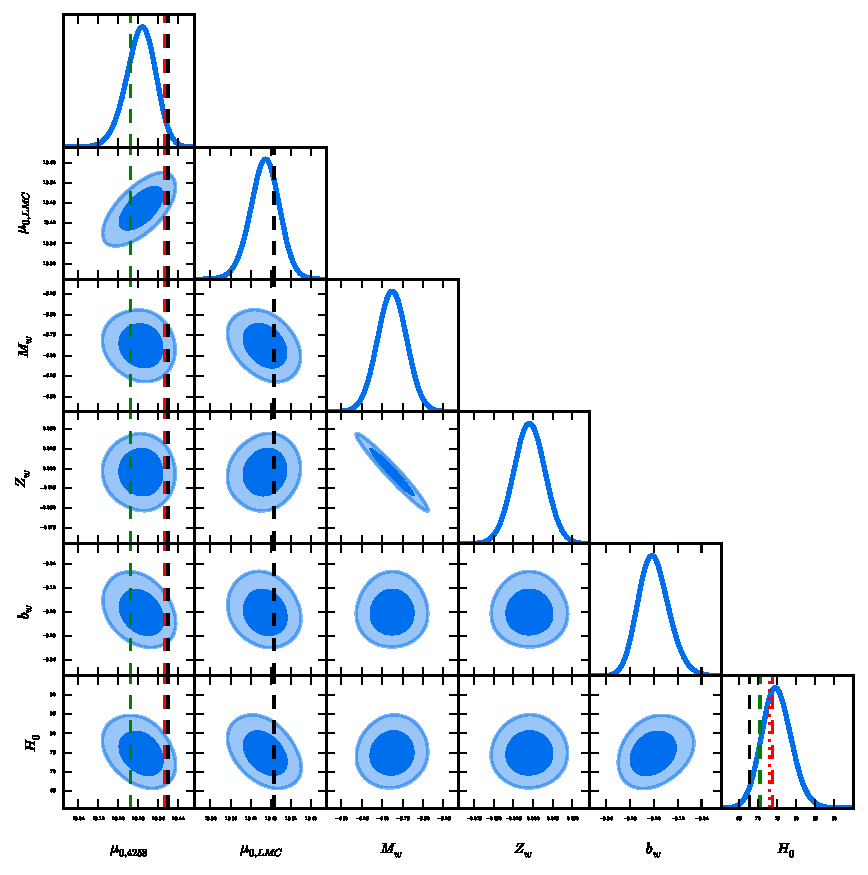
\includegraphics[width=\textwidth]{figures/chapter-h0/triangle_plot.pdf}
\caption{Posterior constraints for fit $(29)$ in Table \ref{Table:Constraints-main-analysis}. Green, red and black vertical dashed lines in $\mu_{0,4258}$ column indicate $\NGC$ distance modulus from \cite{Polshaw:2015ika}, \cite{Riess:2016jrr} and \cite{Humphreys:2013eja}, respectively. Black dashed vertical line in $\mu_{0,\LMC}$ column shows LMC distance modulus from \cite{Pietrzynski:2013gia}. Black, green, and red dashed vertical lines in $H_0$ column respectively indicate the values derived by the Planck collaboration for the base six-parameter $\Lambda$CDM model \cite{Ade:2015xua}, Efstathiou's value \cite{Efstathiou:2013via} used by Planck collaboration as a prior, and the $3\%$ measurement reported by \cite{Riess:2011yx}; the red dotted vertical line indicates the best estimate from the analysis in \cite{Riess:2016jrr}.   }
\label{Fig:Main-analysis-fitM1a}
\end{figure}

\begin{figure}[hbtp]
\centering
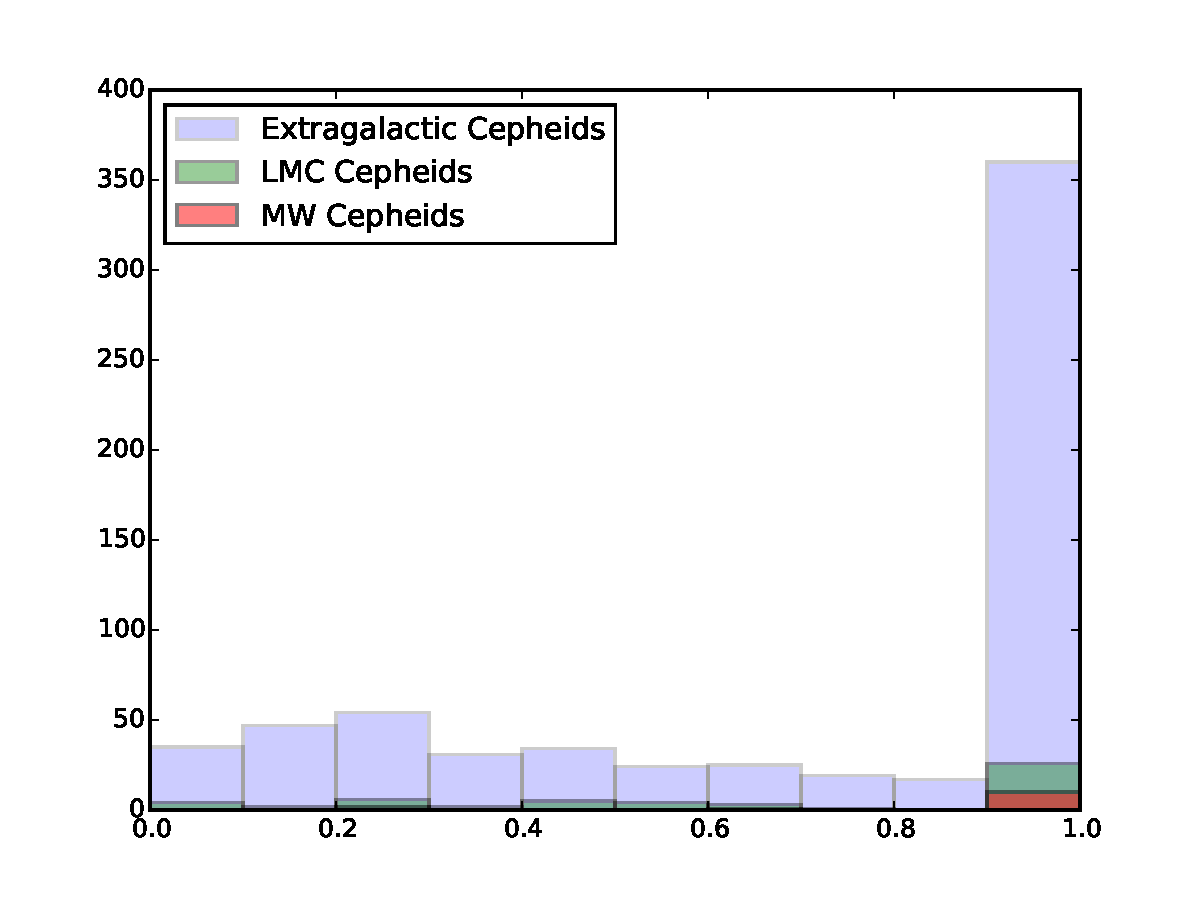
\includegraphics[width=\textwidth]{figures/chapter-h0/effective_HP_histogram.pdf}
\caption{Effective hyper-parameters for the R11 Cepheid sample used in fit $(29)$. From the 646 Cepheid variables in the sample of \cite{Riess:2011yx}, 348 have $\alpha_{\eff}=1$, 263 $10^{-1}\leq \alpha_{\eff} < 1$, 34  $10^{-2}\leq \alpha_{\eff} < 10^{-1}$, and 1 $10^{-3} \leq \alpha_{\eff} < 10^{-2}$. For the 53 LMC Cepheid variables, the analysis outputs 25 $\alpha_{\eff}=1$, 24 $10^{-1}\leq \alpha_{\eff} < 1$, 4  $10^{-2}\leq \alpha_{\eff} < 10^{-1}$. Finally, as for the analysis shown in Figure \ref{Fig:MW-Cepheid-variables}, the set of MW Cepheid variables has 10 stars with $\alpha_{\eff}=1$ and 3 stars with $10^{-1}\leq \alpha_{\eff} < 1$. Overall, $23\%$ of the MW Cepheids are down-weighted. The fraction raises $46\%$ for R11 Cepheids in \cite{Riess:2011yx}. As for the LMC Cepheid variables, the analysis down-weights $53\%$ of the stars.}
\label{Fig:effective-HP-fitM1a}
\end{figure}

\begin{figure}[hbtp]
\centering
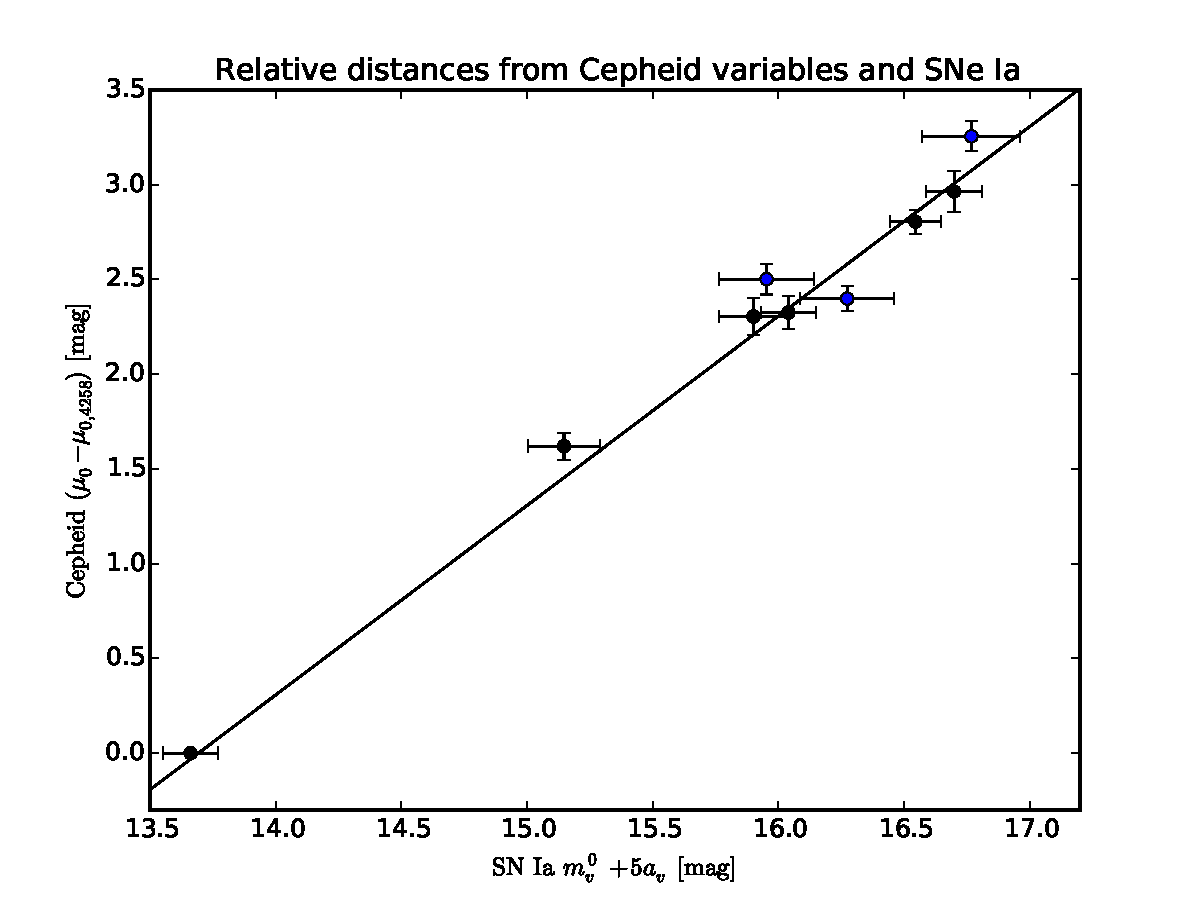
\includegraphics[width=\textwidth]{figures/chapter-h0/effective_HP_SNIa.pdf}
\caption{Relative distances from Cepheids and $\SNe$. We plot the peak apparent visual magnitudes of each $\SNe$ (from Table 3 in \cite{Riess:2011yx}) with error bars rescaled by HPs (colour code is the same as in Figure \ref{Fig:LMC-Cepheid-variables-fit-c}) against the relative distances between hosts determined from fit $(29)$ in Table \ref{Table:Constraints-main-analysis}. The solid line shows the corresponding best fit. The first point on the left corresponds to the expected reddening-free, peak magnitude of an $\SNe$ appearing in the megamaser system $\NGC$ which is derived from the fit $(29)$. }
\label{Fig:HP-SNIa-main-analysis}
\end{figure}

\begin{table}[tbp]
\centering
\begin{tabular}{@{}lccccr}
\hline
\multicolumn{6}{c}{Distance parameters} \\
\hline
Host & SN Ia & $\mu_{0,i}-\mu_{0,4258}$ & $\mu_{0,i} $ best & $\alpha_{\eff}$ & $\sigma_{\intt,i}$\\
\hline

 n4536 & SN 1981B & $1.620\,(0.071)$&$30.91\,(0.08)$ &$1$ & $0.1$ \\

 n4639 & SN 1990N & $2.325\,(0.085)$& $31.61\,(0.09)$& $1 $ & $0.03$\\

 n3370 & SN 1994ae & $2.805\,(0.063)$& $32.09\,(0.07)$& $1 $ & $0.02$ \\
 
 n3982 & SN 1998aq & $2.502\,(0.081)$& $31.79\,(0.08)$& $ 0.23$ & $0.03$\\
  
 n3021 & SN 1995al & $2.964\,(0.110)$& $32.25\,(0.11)$& $ 1$ & $0.03$\\
    
 n1309 & SN 2002fk & $3.255\,(0.079)$& $32.54\,(0.08)$& $ 0.28$ & $0.03$\\

 n5584 & SN 2007af & $2.399\,(0.064)$& $31.69\,(0.07)$& $ 0.43$ & $0.03$\\
       
 n4038 & SN 2007sr & $2.304\,(0.099)$& $31.59\,(0.11)$& $ 1$ & $0.03$\\
       
\hline
\end{tabular}
\caption{\label{Table:SNIa-HP-fit-M1a} Distance parameters for the $\SNe$ hosts corresponding to our primary fit for the R11 data set (fit $(29)$). Numbers in brackets indicate the standard deviation. The last two columns correspond to the effective HP for each $\SNe$ host and the corresponding internal scatter, respectively.}
\end{table}

Fit $(29)$ uses both strong prior on $Z_W$ and no period cut-off in the Cepheid variables sample; it also includes Cepheid stars, $\SNe$ magnitudes, and distance moduli to anchor galaxies with HPs. 
%These choices correspond to the case `$M1^{a}$' of Table \ref{Table:Constraints-main-analysis}. 
We show the parameter constraints for this case in Figure\ \ref{Fig:Main-analysis-fitM1a}. The resulting constraint on the Hubble parameter, which is also our primary fit of the expansion rate derived with the R11 sample of Cepheids, is
\begin{equation}\label{Eq:H0-value-standard-analysis}
	H_0 = 75.0 \pm 3.9 \, \km\, \second^{-1}\, \Mpc^{-1} \, .
\end{equation}
The dashed vertical lines in the 1D marginal posterior for $H_0$ of Figure \ref{Fig:Main-analysis-fitM1a} give (from left to right) the mean values of the Planck $\Lambda$CDM determination of $H_0$ ($67.8\pm0.9\, \km\, \second^{-1}\, \Mpc^{-1}$ from Planck temperature and lensing data \cite{Ade:2015xua}) 
and of the analyses of \cite{Efstathiou:2013via} ($70.6\pm3.3\, \km\, \second^{-1}\, \Mpc^{-1}$), \cite{Riess:2016jrr} ($73.0\pm1.8\, \km\, \second^{-1}\, \Mpc^{-1}$), and \cite{Riess:2011yx} ($73.8\pm2.4\, \km\, \second^{-1}\, \Mpc^{-1}$). Our result here agrees best with the latter two (although our width is somewhat larger due to the use of hyper-parameters), but even the Planck value lies within our $95\%$ credible interval. Note that as the HP likelihoods have wide wings and are very non-Gaussian, one could expect that also the likelihood for $H_0$ is very
non-Gaussian. We found however that it is relatively close to a normal pdf.

Figure \ref{Fig:effective-HP-fitM1a} shows a histogram for HPs in the sample of Cepheid variables used in our primary fit for the R11 data set (fit $(29)$). Whereas in \cite{Riess:2011yx} about $20\%$ of the Cepheids are rejected by the Chauvenet's criterion (this would be equivalent to $\alpha_{\eff}=0$ in our analysis), our analysis finds that about $46\%$ of the Cepheid variables in \cite{Riess:2011yx} are down-weighted ($\alpha_\eff <1$). The analysis in \cite{Riess:2016jrr}, also using a Chauvenet's criterion, finds an outlier fraction of $2\%$ in a larger sample of Cepheid variables. In the next Subsection \ref{Subsection:combining-anchors-R16} we analyse this enlarged Cepheid sample by using HPs. 

Figure \ref{Fig:HP-SNIa-main-analysis} and Table \ref{Table:SNIa-HP-fit-M1a} bring about the presence of possible outliers among the sample of $\SNe$ hosts, thus justifying our use of HPs in the apparent visual magnitudes of each $\SNe$. This could be a hint of unaccounted systematics in the light-curve fits for those $\SNe$. Note that \cite{Riess:2016jrr} has used a different light-curve fitting algorithm (SALT-II) to that utilised in \cite{Riess:2011yx} (MLCS2k2) finding no evidence for any of their $19$ $\SNe$ hosts to be an outlier. We will investigate this claim further in Subsection \ref{Subsection:combining-anchors-R16}.  
 
As mentioned above, the available distance moduli are included with HPs in our primary fit. The resulting effective HPs are: $\alpha^{\eff}_{\LMC}=1$, $\alpha^{\eff}_{\NGC}=0.58$. This shows that the geometric maser distance estimate to the active galaxy $\NGC$ from \cite{Humphreys:2013eja} is slightly down-weighted in our analysis.  As can be seen from the vertical, red, dashed line in Figure \ref{Fig:Main-analysis-fitM1a}, the revised maser distance to $\NGC$  from \cite{Riess:2016jrr} is now closer to our $68\%$ confidence region.     

We also note that it is not least the difference between the supernova distance \cite{Polshaw:2015ika} and
the maser distance \cite{Humphreys:2013eja} to $\NGC$ that limits the precision on $H_0$ as can be seen from the vertical dashed lines
for $\mu_{0,\NGC}$ in Figure \ref{Fig:Main-analysis-fitM1a}. Especially the very recent supernova distance prefers a higher $H_0$ as can be seen
from the marginal 2D likelihood for $\mu_{0,\NGC}$ and $H_0$. An improvement in the anchors is thus important for future improvements in the
direct determination of the local expansion rate $H_0$. %Note, however, that our 'standard analysis' is almost unaffected by the inclusion of the supernova distance \cite{Polshaw:2015ika} to the megamaser system NGC 4258. Fit '$M1^{af}$' includes only the geometric maser distance \cite{Humphreys:2013eja} and we find changes in $H_0$ and $M_W$ smaller than $0.2\%$ w.r.t our 'standard analysis'.

The last three columns in Table \ref{Table:Constraints-main-analysis} show the normalised weight of $j\mathrm{th}$ kind of data  defined as 
\begin{equation}
|| \alpha^{j} || \equiv \frac{\sum_{i=1}^{K_j} \alpha_{i,j}}{K_j},
\label{Eq:normalised-weights}
\end{equation} 
where $\alpha_{i,j}$ denotes $i\mathrm{th}$ HP of kind of data $j$ ($j=\Cepheid,\,\SNe,\,\Anchors$), and $K_j$ stands for the number of objects of kind $j$. When the normalised weight of a given kind of data equals one, it means their reported error bars are all `reliable' in the sense they do not require to be rescaled by HPs (given the best fit parameters). In other words, it gives an idea of how compatible both model and data are. We could also use these normalised weights to asses compatibility of the whole data set. For our particular case of three kinds of data, and as long as $\sum_j|| \alpha^{j} ||\neq 3$, the most compatible fit would be that with $max(\sum_j|| \alpha^{j} ||)$. This happens to be the case for our primary fit $(29)$, for which  $\sum_j|| \alpha^{j}||=2.25$. 

We have also considered variants of the general analysis presented thus far in this section including the three anchor distances available in the R11 data set. They correspond to fits $(31)$--$(33)$ and fit $(35)$ in Tables \ref{Table:details-fits}--\ref{Table:Constraints-main-analysis}. Differently to fit $(34)$, where we use internal scatter nuisance parameters $\sigma_{\intt}$ for each galaxy containing Cepheid variables, in fit $(35)$  we have fixed those nuisance parameters to the values in fit $(75)$ of \cite{Efstathiou:2013via} and used HPs only for the Cepheid variables. The constraints output by two analyses agree within error bars; in particular, the values of $H_0$ agree pretty well. Because the role of $\sigma_{\intt}$ is a common increment of the error bars in the magnitudes of Cepheid variables, a big internal scatter $\sigma_{\intt}$ would mean no Cepheid variables down-weighted by HPs. In fit $(35)$ the internal scatter is five times greater than in fit $(34)$ and as a result all HPs equal $1$. The use of HPs does not weaken the quality of the data as a whole, instead the method is able to identify and down-weight only inconsistent data points. 
 
In Figure \ref{Fig:H0-values-3-anchors} we show our primary fit $(29)$ along with fits $(31)$--$(33)$ and different measurements of the Hubble parameter which use three anchor distances done by other groups. The precision of the measurement using HPs depends on the assumptions made (e.g., including $\SNe$ with HPs, including distance moduli with HPs). The normalised weights for fits including three anchor distances do not suggest dropping the HPs in any kind of data as they never equal $1$ in the fits $(29),\,(34),\,(36)$--$(39)$. Our primary fit and its variants agree with previous measurements \cite{Riess:2011yx} and \cite{Efstathiou:2013via} using the same data set. While analyses using HPs agree with both most recent direct local measurement of $H_0$ \cite{Riess:2016jrr} and the WMAP 2009 indirect determination \cite{Hinshaw:2012aka}, our result is in disagreement with the indirect determination by the Planck collaboration \cite{Ade:2015xua}. The fact that three different analyses converge at similar values for $H_0$ nicely shows that the result is robust. 

\begin{figure}[hbtp]
\centering
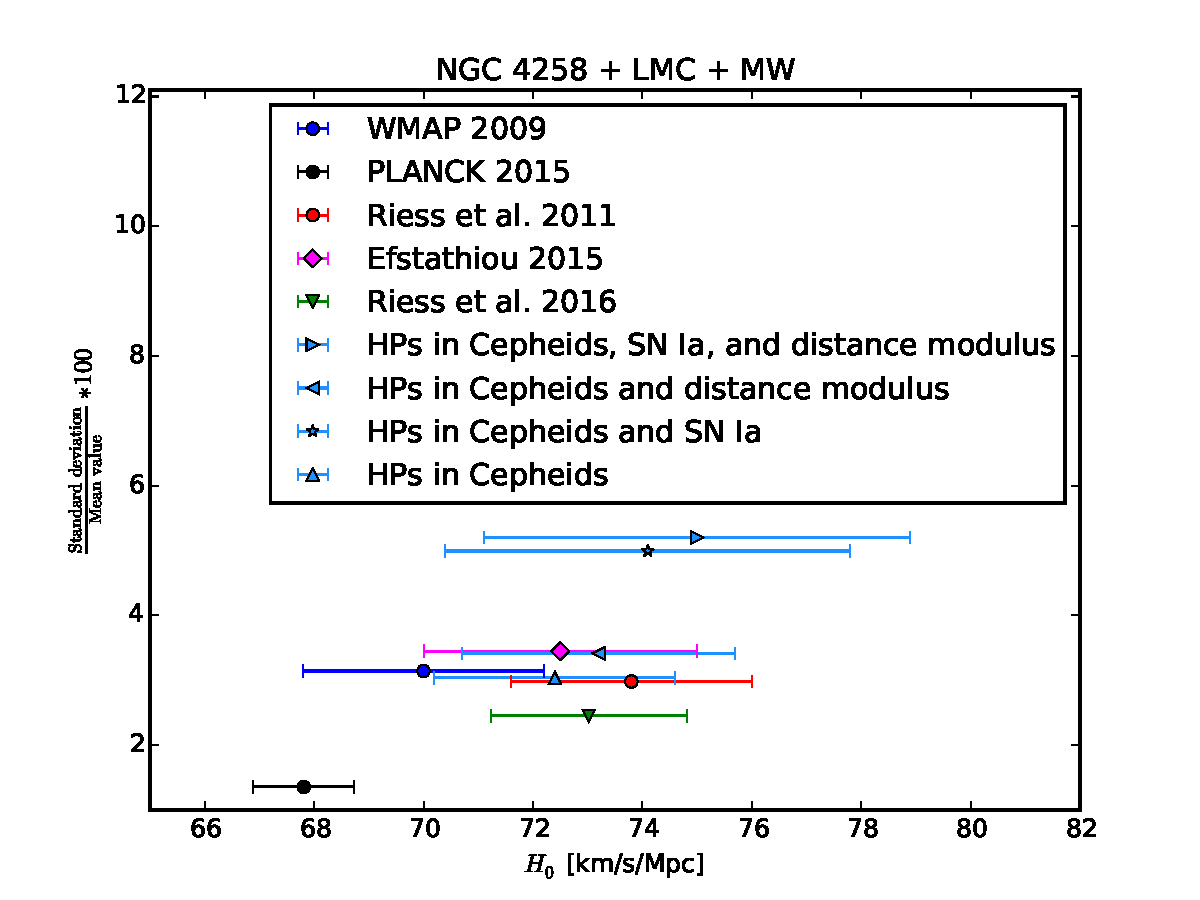
\includegraphics[width=\textwidth]{figures/chapter-h0/H0_values_three_anchors.pdf}
\caption{Different determinations of the Hubble constant. Blue and black show the indirect determinations by the WMAP team \cite{Hinshaw:2012aka} and by the Planck collaboration \cite{Ade:2015xua}, respectively. Direct measurements using NGC 4258 distance modulus, LMC distance modulus and MW Cepheid variables as anchor distances are shown in red, magenta, green, and dodger blue. Red corresponds to measurement by Riess et al. \cite{Riess:2011yx}, magenta shows Efstathiou's measurement \cite{Efstathiou:2013via} which uses a $60$ days period cut, green is the Riess et al. measurement \cite{Riess:2016jrr}, and dodger blue points correspond from top to bottom to fits $(29)$,$(31)$,$(32)$, $(33)$ in Table \ref{Table:Constraints-main-analysis}.\label{Fig:H0-values-3-anchors}}
\end{figure}

Although we have found no reasons to discard any of the data sets, we have carried out analyses simultaneously including only one or two anchors. The cases shown in Table \ref{Table:details-fits}--\ref{Table:Constraints-main-analysis} suggest that i) inclusion of MW Cepheid variables drives $H_0$ to higher values independently of both prior on the metallicity parameter and period cut for period-luminosity relation ii) a strong prior on the metallicity parameter when including distance modulus to LMC also drives $H_0$ to higher values. Figure \ref{Fig:single-combined-anchor} shows the most compatible fits according to the corresponding normalised weights. 
%We discuss this with more details in Appendix \ref{Section:Appendix}.  
 
\begin{figure}[hbtp]
\centering
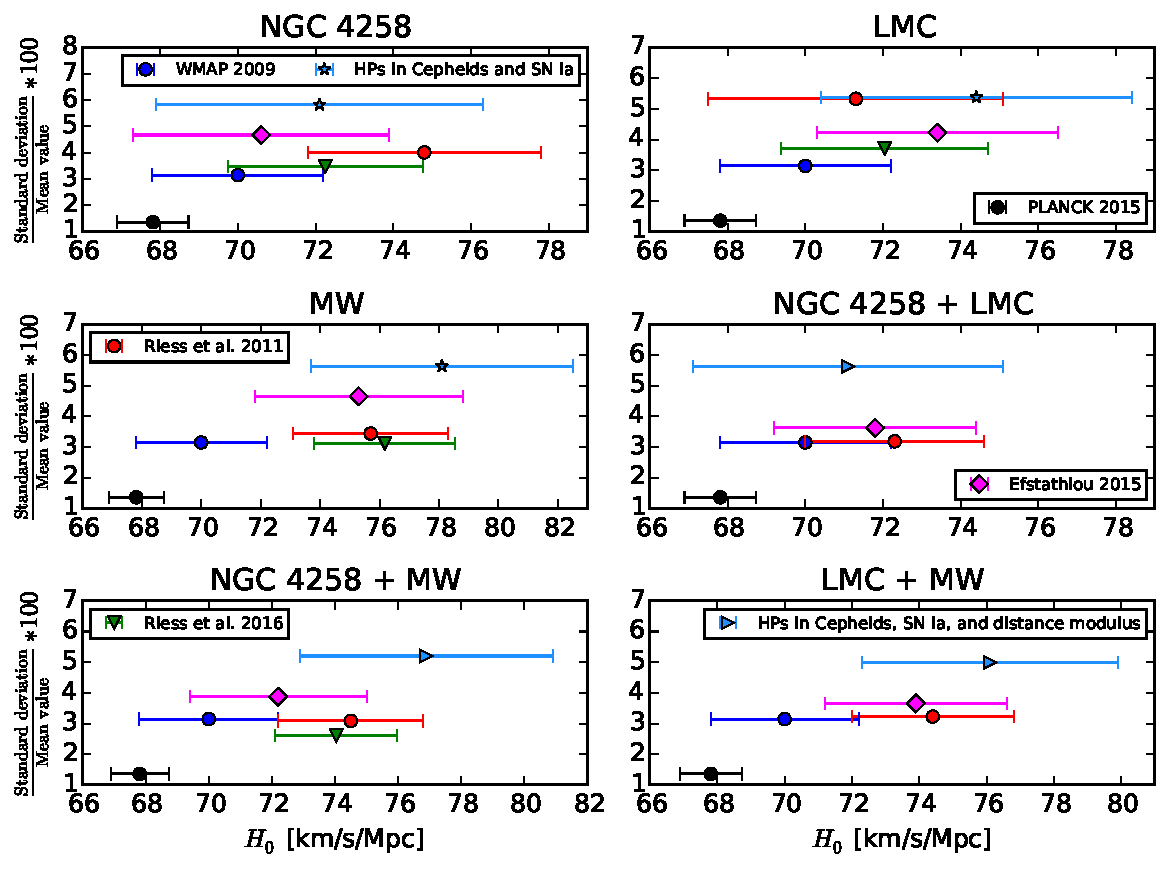
\includegraphics[width=\textwidth]{figures/chapter-h0/H0_values_anchor_combination.pdf}
\caption{Different measurements of the Hubble constant using different combinations of anchor distances. Colours and symbols are as in Figure \ref{Fig:H0-values-3-anchors}. Fits shown are: $(6)\,\NGC$, $(10)\,\LMC$, $(13)\,\MW$, $(17)\,\NGC+\LMC$, $(22)\,\NGC+\MW$, $(28)\,\LMC+\MW$.}
\label{Fig:single-combined-anchor}
\end{figure}

\subsection{Determining $H_0$ with Bayesian hyper-parameters (R16 data set)}
\label{Subsection:combining-anchors-R16}

We now apply HPs to measure the current expansion rate of the universe $H_0$ by using the R16 data set. It comprehends: 
a larger sample of Cepheids in the LMC ($775$ compared to $53$ in R11 data set); $2$ new $\mathit{HST}$-based trigonometric parallaxes for the MW Cepheids (a total of $15$ MW parallaxes, taking into account the $13$ included in the R11 data set); $11$ new $\SNe$ host galaxies (for a total of $19$, taking into account the $8$ in the R11 data set); $\mathit{HST}$ observations of $372$ Cepheid variables in M31 (which were not in the R11 Cepheid sample); the possibility to use $\MAnd$ as an anchor distance taking advantage of the two detached eclipsing binaries based distances to $\MAnd$; $\NGC$ Cepheid stars observed with the same instrument as those in the $19$ $\SNe$ host galaxies, thus reducing the cross-instrument zeropoint errors.   

As we have seen in the previous sections, we do not find any evident reason to discard any of the data sets. In this section we will utilise all available Cepheid data in the R16 data set (including MW Cepheid stars) along with $\LMC$ distance modulus in Eq. \eqref{Eq:LMC-measured-distance-modulus}, $\MAnd$ distance modulus \cite{Riess:2016jrr} given by 
\begin{equation}
\mu_{0,\MAnd}^{\obs} = 24.36 \pm 0.08\, \magn,
\label{Eq:M31-measured-distance-modulus-2016}
\end{equation}
and the improved $\NGC$ distance modulus \cite{Riess:2016jrr}
\begin{equation}
\mu_{0,\NGC}^{\obs} = 29.387 \pm 0.0568\, \magn.
\label{Eq:NGC4258-measured-distance-modulus-2016}
\end{equation}

We have performed the same analysis as for primary best fit with the R11 data set (fit $(29)$ in Table \ref{Table:details-fits}), but also some variants to estimate the impact of used reddening law, period cut-off, metallicity dependence in the R11 data set. Different variants are specified in fits $(40)$--$(55)$ of Table \ref{Table:details-fits} and the corresponding constraints are shown in Table \ref{Table:Constraints-main-analysis}. Changes on the Hubble constant $H_0$ due to different reddening law (different $R$ in Eq. \eqref{Eq:Wesenheit-reddening-free}) range from $0.33$ up to $0.45\, \km\, \second^{-1}\, \Mpc^{-1}$. Differences in the period cut-off produce changes on $H_0$ ranging from $0.06$ to $0.38\, \km\, \second^{-1}\, \Mpc^{-1}$. Allowing for a strong or weak metallicity dependence in the period-luminosity relation we find differences in $H_0$ which range from $0$ to $0.25\, \km\, \second^{-1}\, \Mpc^{-1}$. The standard deviation for measurements of $H_0$ in fits $(40)$--$(55)$ is $\sigma_{\mathrm{syst}}=0.20\, \km\, \second^{-1}\, \Mpc^{-1} $ which we consider as a systematic error due to changes on the reddening law, period cut-off, and metallicity dependence.

According to the normalised weight criterion discussed in Section \ref{Subsection:combining-anchors}, the most compatible fits for the R16 data set are fits $(40),\, (42)$--$(43)$ having $\sum_j || \alpha^{j}||=2.66$ which is higher than that for the R11 data set. For sake of comparison with the best estimate of $H_0$ in \cite{Riess:2016jrr}, we choose fit $(43)$, which uses the same reddening law as best estimate in \cite{Riess:2016jrr}, as our primary fit for the R16 data set. Adding in quadrature the statistical error (quoted in Table \ref{Table:Constraints-main-analysis}) and the systematic error estimated above, we find 
\begin{equation}
H_0 = 73.88 \pm 2.16\,\km\, \second^{-1}\, \Mpc^{-1},
\label{Eq:primary-best-fit-R16}
\end{equation}        
which is a $2.9\%$ measurement of the Hubble constant. The small change in the uncertainty due to inclusion of systematic error shows that HPs are already taking into account most of this contribution to the error budget. 

Figures \ref{Fig:R16-LMC}--\ref{Fig:R16-M31} show period-luminosity relation for best fit of our primary fit $(43)$ for Cepheid stars in galaxies $\LMC,\, \MW,\, \NGC,\, \MAnd$, respectively. Note that no outliers were released in the R16 data set. We find, however, that several Cepheid stars which passed the $2.7\sigma$ outlier rejection criterion in the analysis of \cite{Riess:2016jrr} are down-weighted in our approach. In Figure \ref{Fig:effective-HP-fit-43} we show a histogram for HPs in the R16 Cepheid sample used in fit $(43)$. Differently to our analysis in Section \ref{Subsection:combining-anchors}, which used the R11 data set and included outliers (Cepheid stars which did not pass the $2.5\sigma$ outlier criterion in \cite{Riess:2011yx}), there are no Cepheid stars with $\alpha_\eff<0.1$ in the analysis in this section using the R16 data set. Although outliers in the Riess et al. analysis \cite{Riess:2016jrr} were not released, we find that about $30\%$ of the Cepheid stars in the R16 sample are down-weighted in our analysis. The fraction of down-weighted Cepheid variables was about $46\%$ in our analysis using the R11 data set. Note that the normalised weight for Cepheids increases from $0.72$ for the primary best fit $(29)$ (with the R11 data set) to $0.86$ for the primary best fit $(43)$ (with the R16 data set), which shows that there is an improvement in the compatibility of the data set and therefore a reduction in the fraction of down-weighted stars.    

\begin{figure}[hbtp]
\centering
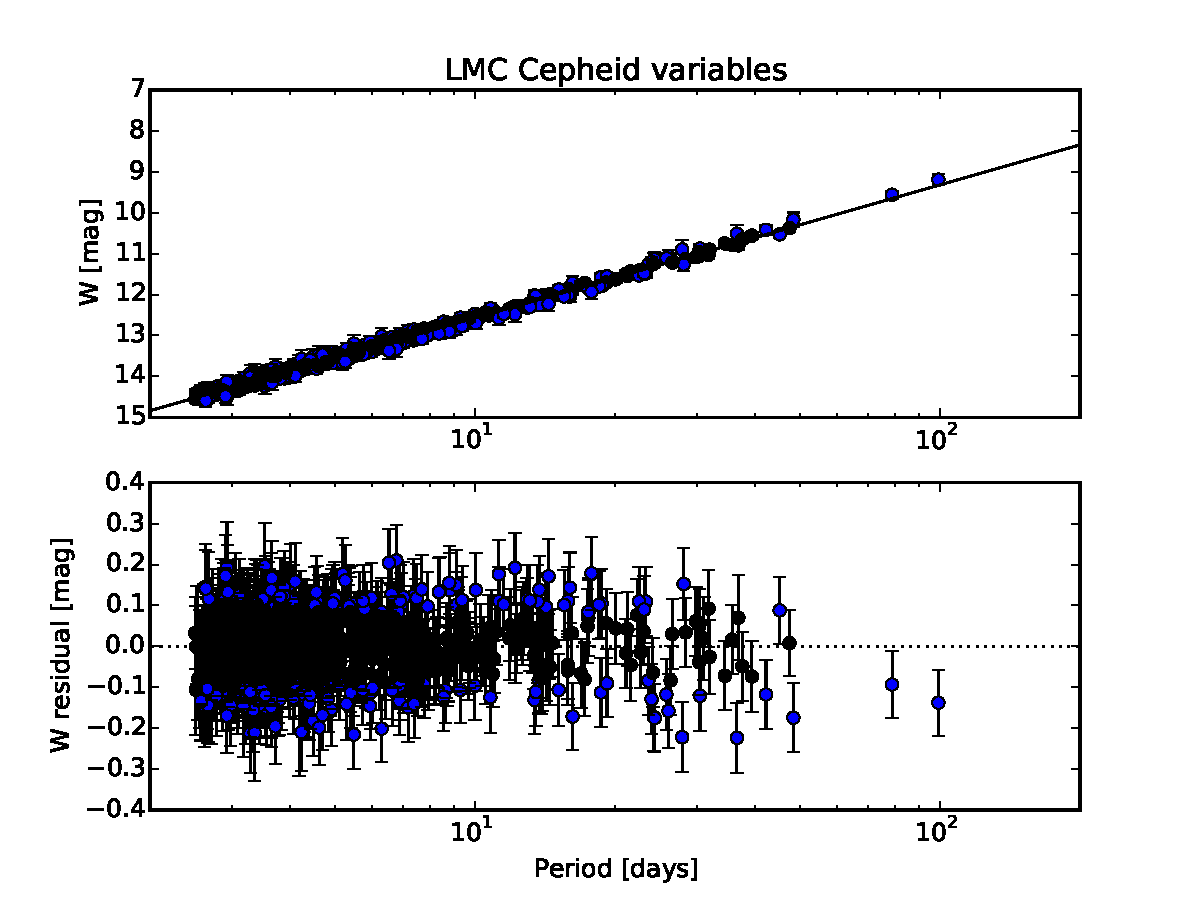
\includegraphics[width=\textwidth]{figures/chapter-h0/effective_HP_cepheids_LMC_R16.pdf}
\caption{Period-luminosity relation (upper panel) and magnitude residuals for the $\LMC$ Cepheid variables in the R16 data set. The solid  shows the best fit of fit $(43)$. In the upper panel we rescale error bars with HPs, in the lower panel we do not. Datums are colour-coded as explained in Figure \ref{Fig:LMC-Cepheid-variables-fit-c}.}
\label{Fig:R16-LMC}
\end{figure}
  
\begin{figure}[hbtp]
\centering
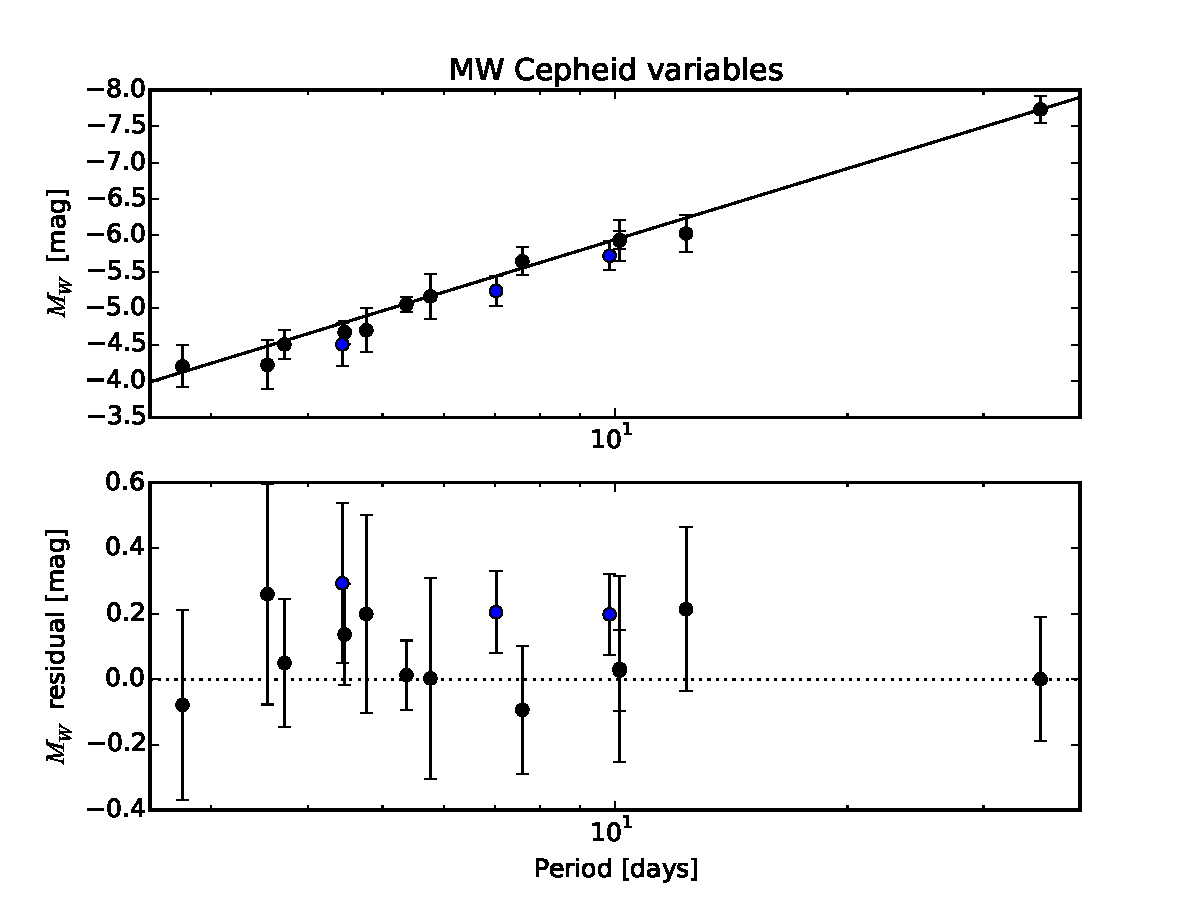
\includegraphics[width=\textwidth]{figures/chapter-h0/effective_HP_cepheids_MW_r16.pdf}
\caption{Period-luminosity relation (upper panel) and magnitude residuals for the $\MW$ Cepheid variables in the R16 data set. The solid  shows the best fit of fit $(43)$. In the upper panel we rescale error bars with HPs, in the lower panel we do not. Datums are colour-coded as explained in Figure \ref{Fig:LMC-Cepheid-variables-fit-c}.}
\label{Fig:R16-MW}
\end{figure}

\begin{figure}[hbtp]
\centering
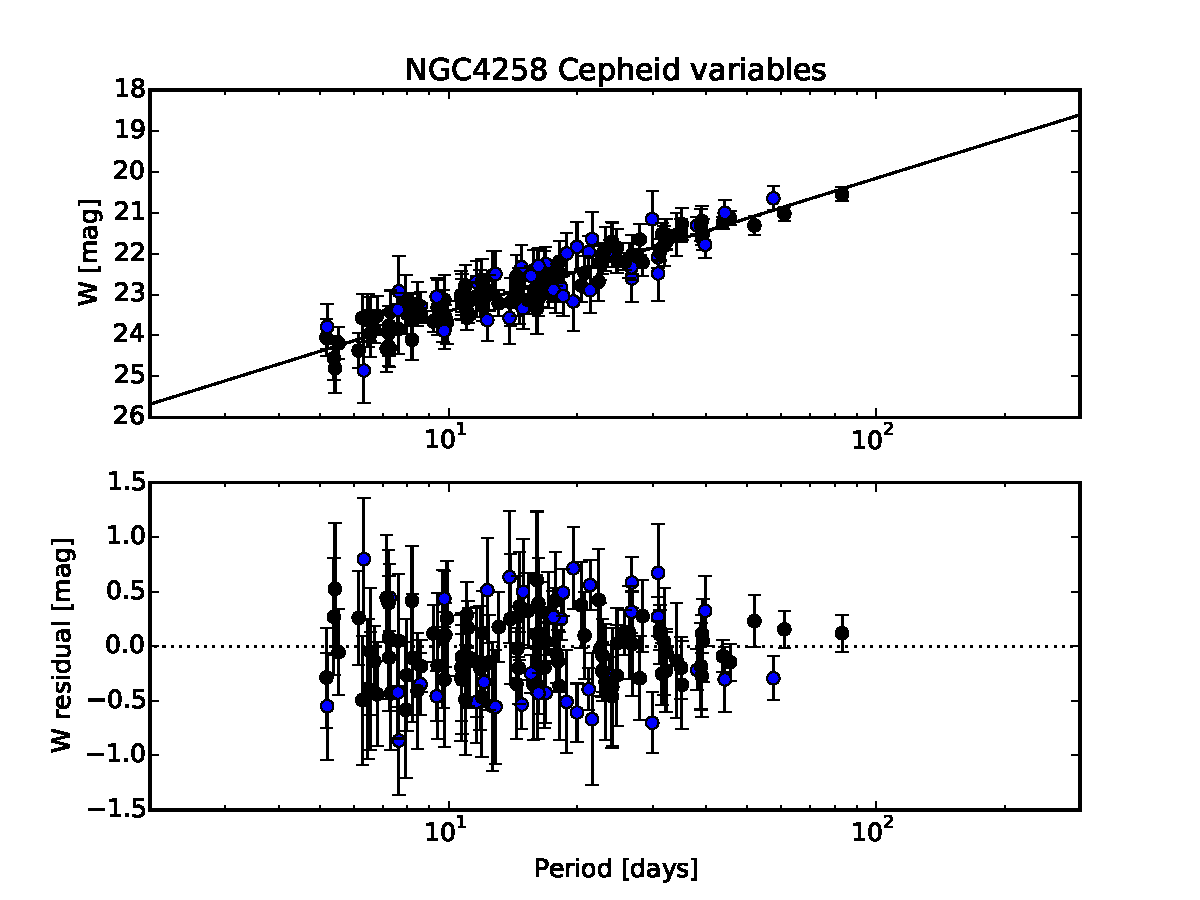
\includegraphics[width=\textwidth]{figures/chapter-h0/effective_HP_cepheids_NGC4258_R16.pdf}
\caption{Period-luminosity relation (upper panel) and magnitude residuals for the $\NGC$ Cepheid variables in the R16 data set. The solid  shows the best fit of fit $(43)$. In the upper panel we rescale error bars with HPs, in the lower panel we do not. Datums are colour-coded as explained in Figure \ref{Fig:LMC-Cepheid-variables-fit-c}.}
\label{Fig:R16-4258}
\end{figure}

\begin{figure}[hbtp]
\centering
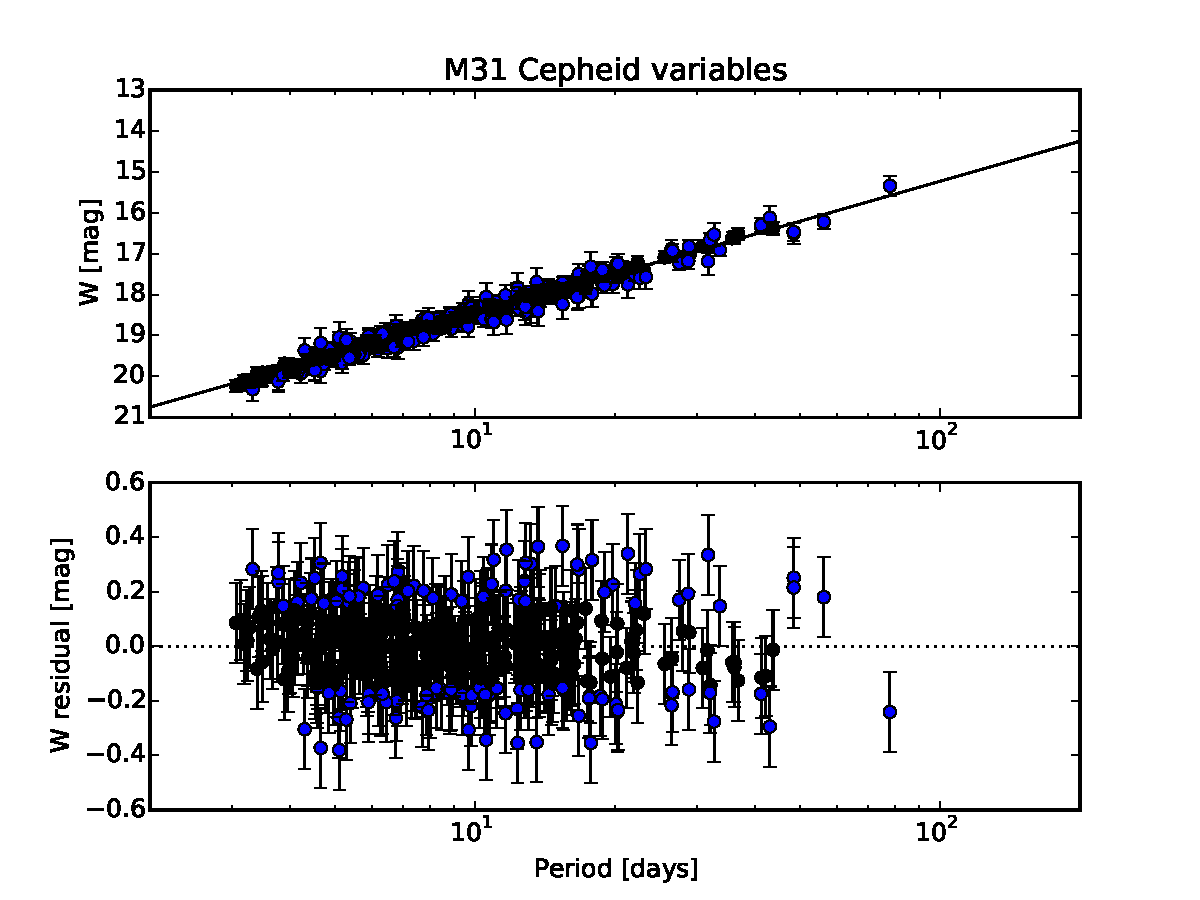
\includegraphics[width=\textwidth]{figures/chapter-h0/effective_HP_cepheids_M31_R16.pdf}
\caption{Period-luminosity relation (upper panel) and magnitude residuals for the $\MAnd$ Cepheid variables in the R16 data set. The solid  shows the best fit of fit $(43)$. In the upper panel we rescale error bars with HPs, in the lower panel we do not. Datums are colour-coded as explained in Figure \ref{Fig:LMC-Cepheid-variables-fit-c}.}
\label{Fig:R16-M31}
\end{figure}

\begin{figure}[hbtp]
\centering
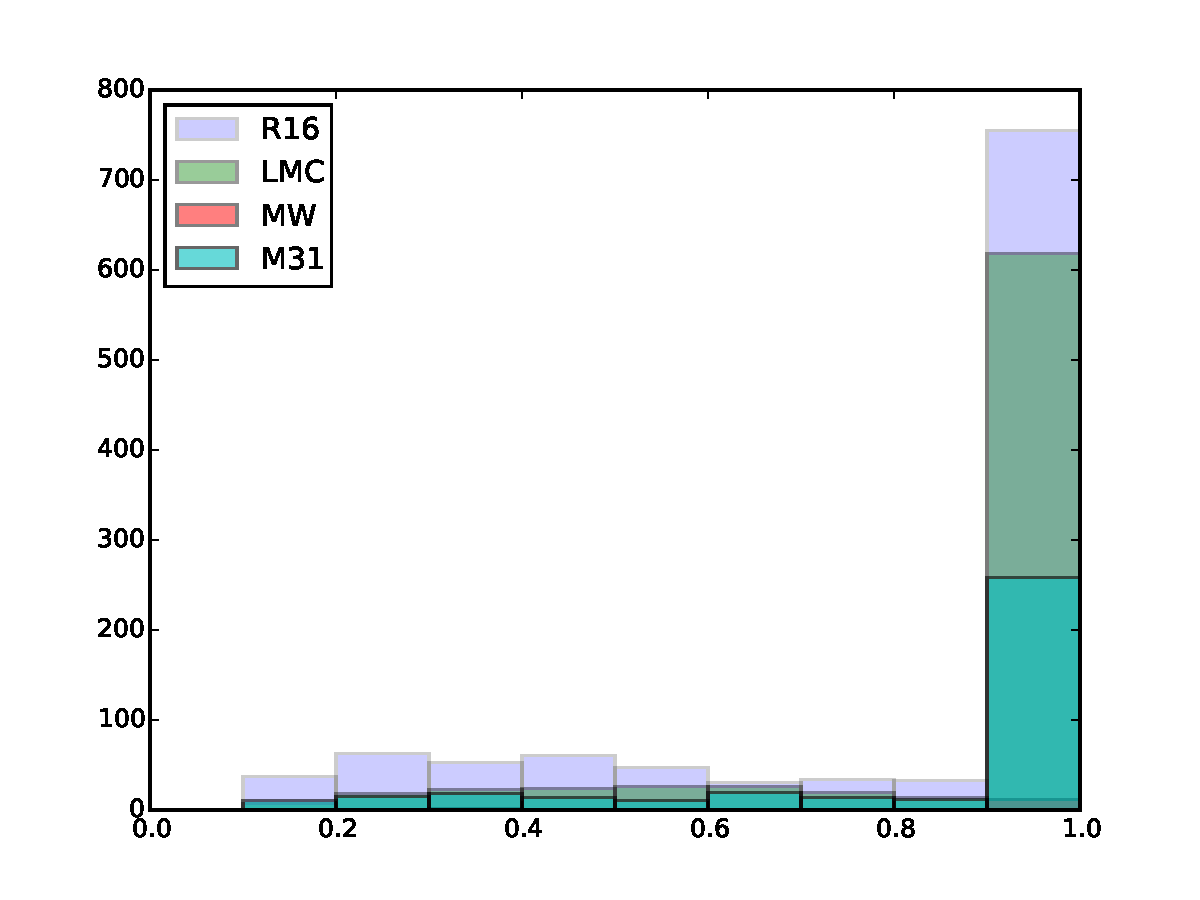
\includegraphics[width=\textwidth]{figures/chapter-h0/effective_HP_histogram_R16.pdf}
\caption{Effective hyper-parameters for the R16 Cepheid sample used in fit $(43)$. From the $1114$ Cepheid variables in the $19$ $\SNe$ host galaxies and in the $\NGC$ megamaser system, $733$ have $\alpha_{\eff}=1$, $381$ $10^{-1}\leq \alpha_{\eff} < 1$, $0$   $\alpha_{\eff} < 10^{-1}$. For the $775$ $\LMC$ Cepheid variables, the analysis outputs $601$  $\alpha_{\eff}=1$, $174$ $10^{-1}\leq \alpha_{\eff} < 1$, $0$  $\alpha_{\eff} < 10^{-1}$. As for the analysis shown in Figure \ref{Fig:MW-Cepheid-variables}, the set of $\MW$ Cepheid variables has $12$ stars with $\alpha_{\eff}=1$ and $3$ stars with $10^{-1}\leq \alpha_{\eff} < 1$. From the $372$ $\MAnd$ Cepheid stars, $249$ have $\alpha_{\eff}=1$, $123$ $10^{-1}\leq \alpha_{\eff} < 1$, $0$   $\alpha_{\eff} < 10^{-1}$. Overall, $20\%$ of the $\MW$ Cepheids are down-weighted; the fraction raises $22\%$ and $33\%$  for $\LMC$ Cepheids and $\MAnd$ Cepheids, respectively; as for the Cepheid variables in the $19$ $\SNe$ hosts and the $\NGC$ system the fraction is $34\%$.}
\label{Fig:effective-HP-fit-43}
\end{figure}

In \cite{Riess:2016jrr} Riess et al., using the SALT-II light curve fitter, found none of the $\SNe$ hosts to be an outlier. Although we cannot claim the opposite, we find that some of the $\SNe$ are down-weighted in our analysis. In Figure \ref{Fig:comparison-distances-R16} we compare the $\SNe$ distances to the approximate, independent Cepheid distances from our primary fit $(43)$. In Table \ref{Table:SNIa-HP-fit-43} we show the distance parameters and the HPs for the $\SNe$ hosts in the R16 data set. The down-weighted $\SNe$ hosts might indicate the presence of unaccounted (or underestimated) systematics in the R16 data set. Whereas our analysis in Section \ref{Subsection:combining-anchors} using R11 data set showed that three out of the eight host galaxies are down-weighted in the fit, the primary fit $(43)$ using the R16 data set down-weights eight $\SNe$ host galaxies. The two host galaxies n3982 and n5584 are down-weighted in both fit $(29)$ and fit $(43)$. From Table \ref{Table:Constraints-main-analysis} we see that the normalised weight for $\SNe$ data is a bit greater for the R16 data set ($0.80$) than for the R11 data set ($0.74$) showing an improvement in the compatibility of this kind of data in the R16 sample.

\begin{figure}[hbtp]
\centering
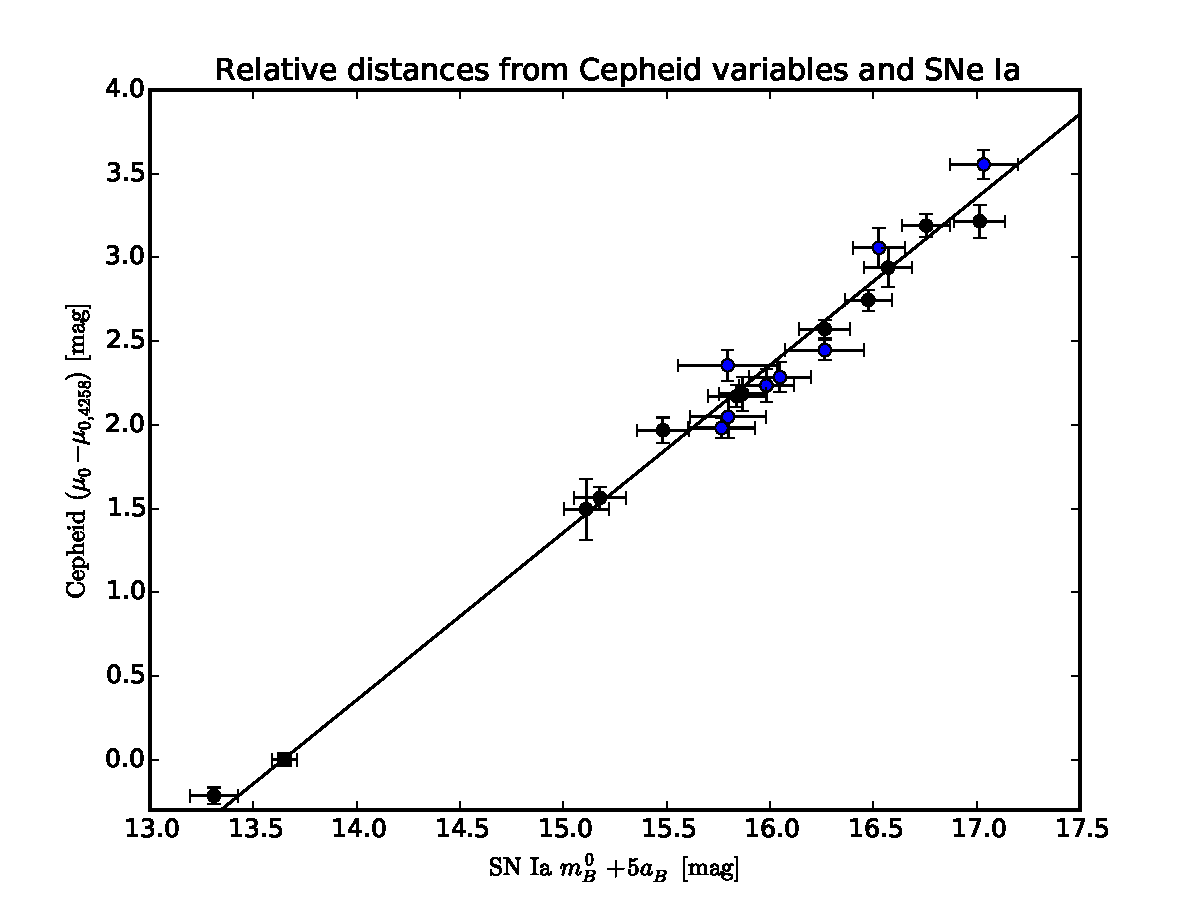
\includegraphics[width=\textwidth]{figures/chapter-h0/effective_HP_SNIa_R16.pdf}
\caption{Relative distances from Cepheids and $\SNe$. We plot the peak apparent visual magnitudes of each $\SNe$ (from Table 5 in \cite{Riess:2016jrr}) with error bars rescaled by HPs (colour code is the same as in Figure \ref{Fig:LMC-Cepheid-variables-fit-c}) against the relative distances between hosts determined from fit $(43)$ in Table \ref{Table:Constraints-main-analysis}. The solid line shows the corresponding best fit. The black square on the left corresponds to the expected reddening-free, peak magnitude of an $\SNe$ appearing in the megamaser system $\NGC$ which is derived from the fit $(43)$.}
\label{Fig:comparison-distances-R16}
\end{figure}

\begin{table}[tbp]
\centering
\begin{tabular}{@{}lccccr}
\hline
\multicolumn{5}{c}{Distance parameters} \\
\hline
Host & $\SNe$ & $\mu_{0,i}-\mu_{0,4258}$ & $\mu_{0,i} $ best & $\alpha_{\eff}$ \\
\hline

 m101 & 2011fe & $-0.215\,(0.049)$&$29.09\,(0.05)$ &$1$ \\
 
 n1015 & 2009ig & $3.216\,(0.100)$&$32.53\,(0.10)$ &$1$ \\

 n1309 & 2002fk & $3.190\,(0.070)$& $32.50\,(0.07)$& $ 1$ \\
  
 n1365 & 2012fr & $1.968\,(0.076)$& $31.28\,(0.08)$& $ 1$ \\
   
 n1448 & 2001el & $1.981\,(0.059)$& $31.29\,(0.06)$& $ 0.52$ \\   
   
 n2442 & 2015F & $2.171\,(0.065)$& $31.48\,(0.07)$& $ 1$ \\
    
 n3021 & 1995al & $3.058\,(0.117)$& $32.37\,(0.12)$& $ 0.86$ \\
     
 n3370 & 1994ae & $2.746\,(0.063)$& $32.06\,(0.07)$& $1 $  \\
      
 n3447 & 2012ht & $2.572\,(0.054)$& $31.88\,(0.06)$& $1 $  \\
 
 n3972 & 2011by & $2.285\,(0.087)$& $31.59\,(0.09)$& $0.60 $  \\ 
 
 n3982 & 1998aq & $2.356\,(0.093)$& $31.67\,(0.09)$& $ 0.23$ \\
  
 n4038 & 2007sr & $2.048\,(0.125)$& $31.36\,(0.13)$& $ 0.39$ \\  
  
 n4424 & 2012cg & $1.497\,(0.182)$& $30.81\,(0.18)$& $ 1$ \\  
  
 n4536 & 1981B & $1.564\,(0.067)$&$30.87\,(0.07)$ &$1$ \\

 n4639 & 1990N & $2.235\,(0.097)$& $31.55\,(0.10)$& $0.75 $ \\
    
 n5584 & 2007af & $2.446\,(0.058)$& $31.76\,(0.06)$& $ 0.37$ \\
       
 n5917 & 2005cf & $2.939\,(0.115)$& $32.25\,(0.11)$& $ 1$ \\
       
 n7250 & 2013dy & $2.185\,(0.102)$& $31.50\,(0.10)$& $ 1$ \\
        
 u9391 & 2003du & $3.555\,(0.087)$& $32.87\,(0.09)$& $ 0.48$ \\
         
\hline
\end{tabular}
\caption{\label{Table:SNIa-HP-fit-43} Distance parameters for the $\SNe$ hosts corresponding to our primary fit [fit $(43)$] for the R16 data set. Numbers in brackets indicate the standard deviation. The last column shows the effective HP for each $\SNe$ host.}
\end{table}

Comparing the normalised weight of anchors in Table \ref{Table:Constraints-main-analysis} for fits $(29)$ and $(43)$ ($0.79$ and  $1$, respectively), one can see an improvement of the compatibility of this kind of data in the R16 data set. Although this would be a hint to not include distance moduli with HPs in the fit (since the HP Gaussian likelihood would add uncertainty having a bit wider wings), we can see that the normalised weight of anchors depends on the variants of the analysis ($R$, period cut-off, metallicity prior) ranging from $0.62$ to $1$ and hence there is no strong reason to exclude the use of HPs in this kind of data. 

Figure \ref{Fig:Best-estimates-H0-R16} shows the best estimates of $H_0$ by G. Efstathiou \cite{Efstathiou:2013via}, Riess et al. \cite{Riess:2011yx}, Riess et al. \cite{Riess:2016jrr}, and those in this work, fits $(29)$ and $(43)$, along with the indirect determinations of $H_0$ by the WMAP team \cite{Hinshaw:2012aka} and by the Planck collaboration \cite{Ade:2015xua}. Our best estimate using the R11 data set, fit $(29)$, is the most uncertain (a $5.2\%$ measurement) of all presented measurements, but it agrees with all previous direct determinations of $H_0$ and differs by $1.8\sigma$ from the Planck value. Note that because G. Efstathiou considered only $\NGC$ as an anchor and a period cut-off of $60$ days his determination is more uncertain than that of Riess et al. \cite{Riess:2011yx} which used three anchors and no period cut-off. Our best estimate using the R16 data set, fit $(43)$, also agrees with all previous, shown, direct determinations of $H_0$ and its uncertainty is smaller (a $2.9\%$ measurement) than that in fit $(29)$. Concerning the indirect determinations of $H_0$, we see that our best estimate, fit $(43)$, agrees within $1\sigma$ with WMAP 2009, but it is in $2.6\sigma$ disagreement with the Planck value. This tension might be a hint of unresolved systematics in CMB data \cite{Riess:2016jrr}. 

\begin{figure}[hbtp]
\centering
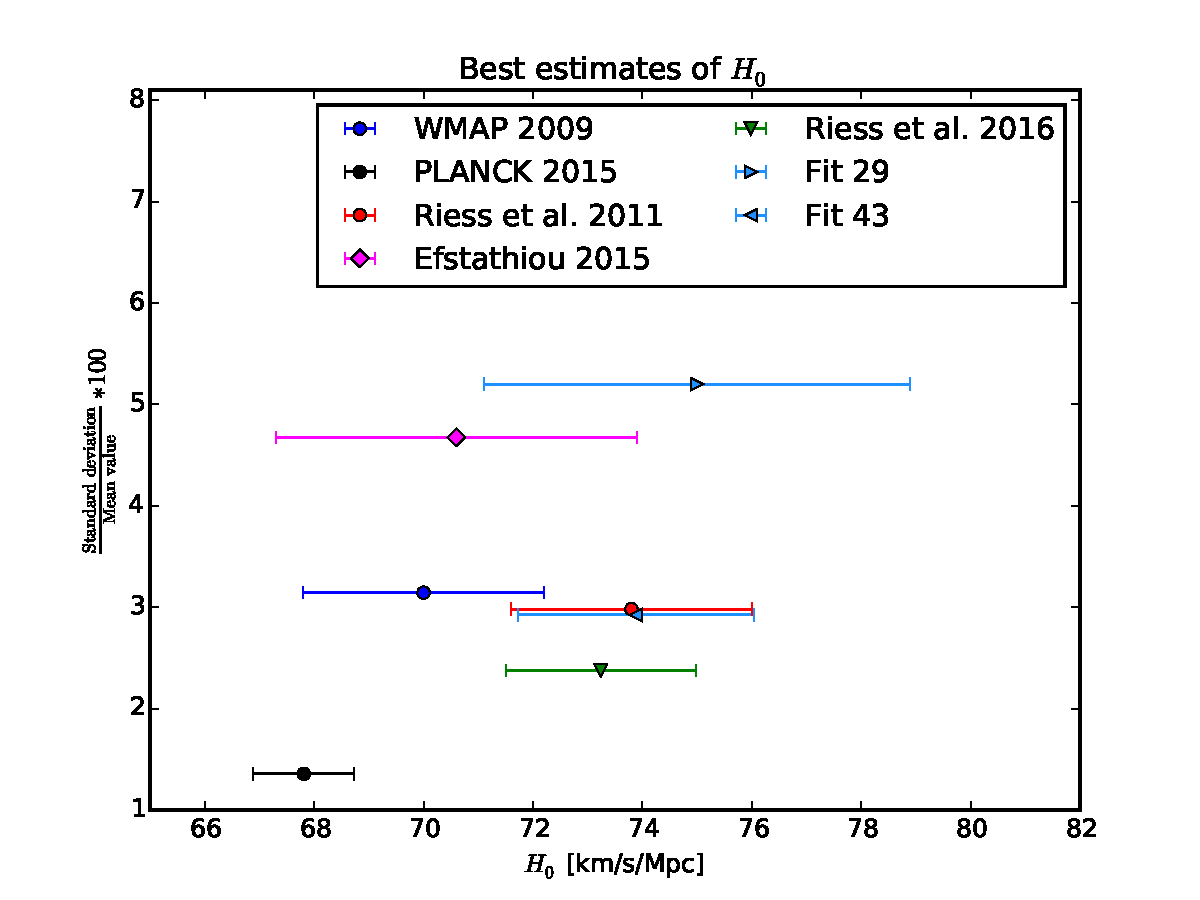
\includegraphics[width=\textwidth]{figures/chapter-h0/H0_best_values_R16.pdf}
\caption{Best estimates of the Hubble constant. Blue and black show the indirect determinations by the WMAP team \cite{Hinshaw:2012aka} and by the Planck collaboration \cite{Ade:2015xua}, respectively. Direct measurements using $\NGC$ distance modulus, $\LMC$ distance modulus and $\MW$ Cepheid variables as anchor distances are shown in red and green; red corresponds to measurement by Riess et al. \cite{Riess:2011yx}, whereas green shows measurement by Riess et al. \cite{Riess:2016jrr}. Magenta shows Efstathiou's measurement \cite{Efstathiou:2013via} which uses only $\NGC$ as anchor distance and a $60$ days period cut-off. In dodger blue we show best estimates for both R11 and R16 data sets, fits $(29)$ and $(43)$ in Table \ref{Table:Constraints-main-analysis}, respectively.}
\label{Fig:Best-estimates-H0-R16}
\end{figure}


\section{Discussion and Conclusions}
\label{chapter-h0:Summary}

In the previous Section we presented an statistical method which allows a comprehensive treatment of available data to determine the universe's current expansion $H_0$. The use of Bayesian hyper-parameters avoids the arbitrary discard of data which is implicit in outlier rejection algorithms. Such algorithms have been used in  \cite{Riess:2009pu}, \cite{Riess:2011yx}, \cite{Efstathiou:2013via} and in some cases a dependence of the results with the statistical method utilised has been found. The determination of the Hubble constant with Bayesian hyper-parameters is robust against different assumptions in the analysis (e.g., period cut in the Cepheid variables data, prior on the metallicity parameter $Z_W$ of the period-luminosity relation, reddening law) as can be seen from Table \ref{Table:Constraints-main-analysis}. In addition, since the method utilises all available data sets, it allows to check how consistent with each other they are and how much weight they are assigned in the fit. Low values of HPs might be due to unrecognised (or underestimated) systematics in the data sets or might be a calling for better modelling.

We have shown that, contrary to an usual $\chi^2$ approach, when Cepheid variables are fitted using HPs, the down-weighted datums (outlier candidates in an outlier rejection algorithm) do not significantly bias the slope $b_W$ in the period-luminosity relation (see Figure \ref{Fig:LMC-Cepheid-variables-fit-c} and Table \ref{Table:LMC-fits}). Note that due to degeneracies in the parameters (e.g., $H_0,\, M_W,\, b_W,\, Z_W,\,$\dots), this could also lead to bias in the determination of the Hubble constant $H_0$ in an usual $\chi^2$ analysis. Moreover, a decrement of the data set might lead to unnecessary increase of the error bars in the fitting parameters (compare, for instance, Efstathiou \cite{Efstathiou:2013via} and Riess et al. \cite{Riess:2011yx} $H_0$ values in Figure \ref{Fig:Best-estimates-H0-R16}).

From Subsections \ref{Subsection:LMC}--\ref{Subsection:NGC4258} it becomes clear that the three set of Cepheid variables in the galaxies LMC, MW, and NGC 4258 are consistent with each other ($b_W$ and $M_W$ agree within error bars) thus providing no argument to exclude any of them from the main analysis. In Subsection \ref{Subsection:Zw-dependence} we have studied the period-luminosity relation -- allowing for a metallicity dependence -- of each one of the galaxies in the R11 data set containing Cepheid variables. Table \ref{Table:Zw-dependence-of-PL-relation} shows that at least five galaxies have an slope $b_W$ which differs from that of LMC Cepheid variables by about $2\sigma$. An statistical method combining these data sets without taking those inconsistencies into account could lead to biased results (compare, for instance, $b_W$ for our fits in Table \ref{Table:Constraints-main-analysis} with the corresponding fits in Appendix A of \cite{Efstathiou:2013via} which are driven upwards). Our method is able to deal with those data sets thus no biasing our constraints in the period-luminosity parameters.

One of the advantages of using HPs to determine the Hubble constant is that one can assess the compatibility of different data sets. Our best estimates, fits $(29)$ and $(43)$, include with HPs available Cepheid variables (i.e., no period cut), available independent measurements of distance modulus to $\NGC$, $\LMC$, and $\MAnd$ [only in fit $(43)$], and available $\SNe$ apparent magnitudes, but we have also performed several variants which are shown in Table \ref{Table:Constraints-main-analysis}. %In Table \ref{Table:HPs-main-analysis-Table3} we show the HPs for the available distance modulus and the sum of effective HPs for both SNe Ia hosts and MW Cepheid variables corresponding to fits in Table \ref{Table:Constraints-main-analysis}. Fits that only differ from the 'standard analysis' either in the period cut or in the prior for the metallicity parameter $Z_W$ give consistent results: we obtain a $5\%$ measurement of $H_0 \approx 75 \pm 4\, \km\, \second^{-1}\, \Mpc^{-1}$. Differently to the 'standard analysis', the fit '$M1^{af}$' does not include the distance modulus to NGC 4258 from \cite{Polshaw:2015ika}. This change does not considerably change the constraints, but whereas MW Cepheid variables gain a bit of weight in the analysis, both SNe Ia hosts and distance modulus to NGC 4258 are more down-weighted than in the 'standard analysis'. In fact, SNe Ia hosts show the lowest degree of agreement among the different variants of fit '$M1^a$'.
We have estimated the degree of agreement for different kind of data in our fits through the normalised weights \eqref{Eq:normalised-weights} and found that fits $(29)$ and $(43)$ provide the best solution for R11 and R16 data sets, respectively. Although no outliers were released in the R16 data set, the HP analysis down-weights some of the Cepheid stars which passed the outlier rejection algorithm in \cite{Riess:2016jrr}. Our analysis also shows hints of possible underestimated uncertainties in the $\SNe$ magnitudes of both R11 and R16 data sets.   

Since our analysis shows down-weighted datums in available data sets, we think an analysis with HPs is appropriate. The analysis is safe because it does not bias the results in the presence of datums with unreliable error bars. The use of HPs is conservative because it does underestimate the error bars on the constraints. Moreover, HPs are useful because they suggest the presence of possible underestimated systematics in the data. We conclude that as long as the sum of normalised weights \eqref{Eq:normalised-weights} for the three kinds of data $\sum_j || \alpha^j || \neq 3$,  HPs offer a reliable approach to measure the universe's expansion rate. In a fully compatible case for which $\sum_j || \alpha^j || = 3$ an usual $\chi^2$ approach could be adopted and find constraints with smaller error bars than those in a HP approach.  

%In the fit '$M1^{ag}$' the value of the Hubble constant is shifted downwards by $\approx 2\%$ w.r.t. our 'standard analysis'. In this case we do not include SNe Ia hosts with HPs; This would be equivalent to assume that there are no outliers among the SNe Ia hosts assigning thus equal weight to every host galaxy in the analysis. Although this assumption both brings the distance modulus to NGC 4258 from \cite{Humphreys:2013eja} in better agreement and decreases the standard deviation in $H_0$ (it is now a $3\%$ measurement), our main analysis brings about the presence of down-weighted SNe Ia hosts (see Figure \ref{Fig:HP-SNIa-main-analysis}). Such an assumption is implicit in the analyse \cite{Riess:2011yx} and \cite{Efstathiou:2013via}. Presence of outliers among the SNe Ia hosts might be due to unaccounted (or underestimated) systematics in the light-curve fits for those SNe Ia. In \cite{Riess:2016jrr} a new, enlarged sample of $18$ SNe Ia hosts has been fitted with the SALT-II algorithm (instead of MLCS2k2 used by \cite{Riess:2011yx}) finding no evidence for outliers. Once the data becomes available, this could be easily verified with our method.

%We have also studied the possibility of including the available distance modulus with equal weight in the fit, but using HPs in the SNe Ia hosts. This corresponds to the fit '$M1^{ah}$' which gives a value of $H_0$ ($5\%$ measurement) lower than in our 'standard analysis' by $\approx 1\%$. In this case the SNe Ia hosts are less down-weighted than in any other variant of fit '$M1^a$'.

%In the fit '$M1^{aj}$' we have only used HPs in the Cepheid variables. This case is close to the analysis of \cite{Riess:2011yx} where they found $H_0 = 73.8 \pm 2.1 \, \km\, \second^{-1}\, \Mpc^{-1}$ the difference being the inclusion of all the available Cepheid variables (no outlier rejection applied) in fit '$M1^{aj}$'. Although the uncertainties output by the two analyses are almost the same, our $H_0$ value is lower than theirs by $\approx 2\%$. Our $H_0$ value agree better with fits $75$, $79$, and $83$ of \cite{Efstathiou:2013via} which use both period cut and outlier rejection, though.

%Fit '$M1^b$' differs from '$M1^a$' in the use of a smaller subset of Cepheid variables (upper period cut of $60$ days). While the distance modulus to NGC 4258 from \cite{Humphreys:2013eja} gets down-weighted, the compatibility of the MW Cepheid variables is enhanced.






%\begin{table}[tbp]
%\centering
%\begin{tabular}{@{}lccccc}
%\hline
%\multicolumn{6}{c}{NGC $4258$ $+$ LMC $+$ MW anchors} \\
%\hline
%Fit & $\alpha_{4258}^{\eff,\,\rm M1}$ & $\alpha_{4258}^{\eff,\,\rm M2}$ & $\alpha_{\LMC}$ & $\sum_{i=1}^{8}  \alpha^{\eff,\,\SNe}_{i}$ &$\sum_{i=1}^{13} \alpha^{\eff,\,\MW}_{i}$ \\
%\hline
%$M1^{a}$ & $ 0.6 $ & $ 1 $ & $ 1 $ & $ 5.9 $ & $ 11.2 $ \\
%$M1^{af}$ & $ 0.5 $ & $ $ & $ 1 $ & $ 5.4 $ & $ 11.4 $ \\
%$M1^{ag}$ & $ 0.8 $ & $ 1 $ & $ 1 $ & $ $ & $ 11.1 $ \\
%$M1^{ah}$ & $ $ & $ $ & $ $ & $ 6.5 $ & $ 11.5 $ \\
%$M1^{aj}$ & $ $ & $ $ & $ $ & $ $ & $ 11.2 $\\
%$M1^{b}$ & $ 0.3 $ & $ 1 $ & $ 1 $ & $ 5.9 $ & $ 11.9 $ \\
%$M1^{be}$ & $ $ & $ $ & $ $ & $ $ & $ 13 $ \\
%$M2^{a}$ & $ 0.7 $ & $ 1 $ & $ 0.4  $ & $ 6.1 $ & $ 11.2$ \\
%$M2^{b}$ & $ 0.5 $ & $ 1 $ & $ 0.6 $ & $ 5.7 $ & $ 11.3 $ \\
%$M3^{a}$ & $ 0.4 $ & $ 1 $ & $ 0.9 $ & $ 6.3 $ & $ 11.4 $ \\
%$M3^{b}$ & $ 0.9 $ & $ 1 $ & $ 0.2 $ & $ 6.0 $ & $ 11.0 $ \\
%%$M3^{a}$ & $75.0\,(3.9)$ & $-5.92\,(0.04)$ & $-3.20\,(0.05)\,[N]$ & $0$ & $0.06$ & $0.02$ \\
%%$M3^{b}$ & $75.4\,(3.7)$ & $-5.92\,(0.04)$ & $-3.27\,(0.04)\,[N]$ & $ 0 $ & $0.06$ & $0.02$ \\
%\hline
%\end{tabular}
%\caption{\label{Table:HPs-main-analysis-Table3} Effective hyper-parameters for distance modulus used in fits of Table \ref{Table:Constraints-main-analysis} and the sum of effective HPs for both SNe Ia hosts and MW Cepheid variables.%\comment{COMMENT: reminder, change labels M1, M2, renormalise last two columns to 1}}
%}
%\end{table}

\chapter{Outlook}
\label{chapter-outlook}

\addcontentsline{toc}{chapter}{Appendices}  
\chapter*{Appendices}  

\appendix

\chapter{Stability}
\label{appendix1-ade}

The non-autonomous system of coupled differential equations (\ref{eq:de-cont})-(\ref{eq:de-eul}) for density and velocity perturbations can be written as
\be 
\vec{\mathbf{x}}' = \mathbf{B}(a;\theta_j) \, \vec{\mathbf{x}}\, ,
\label{eq:appendix:B1}
\ee
where $ \vec{\mathbf{x}}^\intercal = (\delta_m,\, V_m,\, \delta_{de},\, V_{de}) $, $ \mathbf{B} $ is a $ 4\times4 $ matrix which depends on the parameters $\theta_j=\lcb H_0,\, w,\, \Omega_m,\, \Omega_x,\,  c_s,\, \aa,\, \ff,\, \gg \rcb$, on the mode $ k $ and the scale factor $ a $. In order to obtain information about the parameter space, we assess the stability of the system (\ref{eq:appendix:B1}). We compute the eigenvalues $ \lambda_k (a,\, \theta_j)$ of the matrix $\mathbf{B}(a;\theta_j)$ numerically and look at the regions in the $\theta_j-$space where all eigenvalues have negative real parts for the whole time interval we consider, that is, from matter domination to the present time. 

For the system (\ref{eq:appendix:B1}) we find one eigenvalue which does not have a region in $\theta_j-$space where $\operatorname{Re} \left( \lambda_k (a,\, \theta_j) \right) < 0$. Then, since we know that in matter dominated era and on sub-horizon scales matter perturbations grow linearly, that is, $ \delta_m \propto a$, we use the following approach to assess the stability of the system. First, we rescale the  variables $ \vec{\mathbf{x}} $ dividing them by a power $ a^m $ of the scale factor, $\vec{\mathbf{y}}=a^{-m}\vec{\mathbf{x}}$. It follows that the system  (\ref{eq:appendix:B1}) becomes   
\be
\vec{\mathbf{y}}' = \mathbf{A}(a;\theta_j) \, \vec{\mathbf{y}}\, ,
\label{eq:appendix:B2}
\ee
where $ \mathbf{A}(a;\theta_j) = \mathbf{B}(a;\theta_j) - \frac{m}{a} \mathbf{I}  $, with $ \mathbf{I} $ the identity matrix. Second, we find regions in parameter space where all the eigenvalues of the matrix $ \mathbf{A} $ have negative real parts. We study models with $ \aa=\gg=0 $ since the effective sound speed $ \ceff^2 $ is only defined in terms of $ c_s $ and $ \ff $;  moreover we check the robustness of our method with different powers $ m $. Fig. \ref{fig:stability} shows regions where all eigenvalues have real part negative in the time interval relevant for both super and sub-horizon scales.  Since we use $ c_s^2=1 $ we can see clearly an upper limit on $ \ff =3/2$, which nicely agrees with $ \ceff^2>0 $.  

\begin{figure}[tb]
\centering
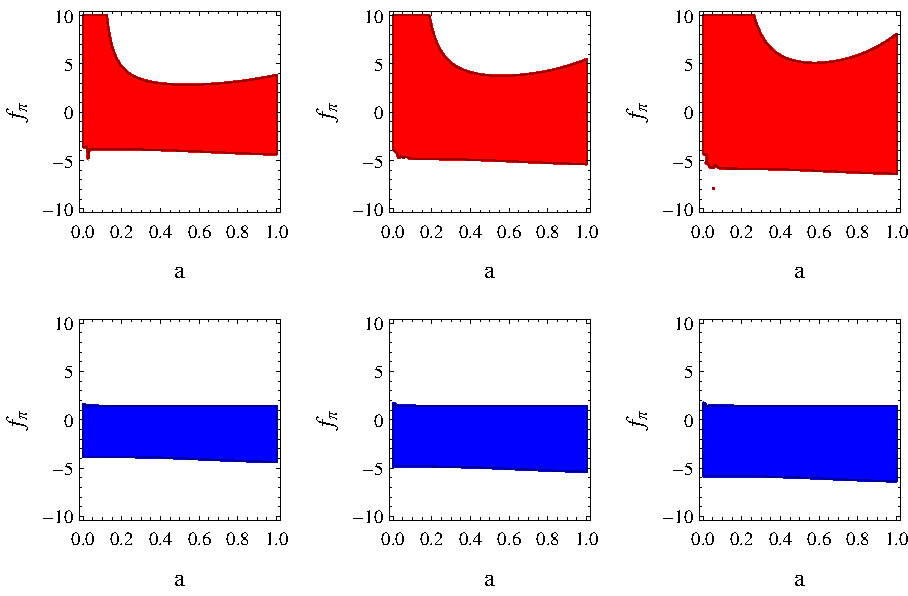
\includegraphics[width=\textwidth]{figures/chapter-ade/stability.pdf} 
\caption{The figure shows the region in the $ \ff-$space for which all the eigenvalues of the matrix $ \mathbf{A} $ in Eq. (\ref{eq:appendix:B2}) have negative real parts. The red region (upper panel) corresponds to a mode on super-horizon scales ($k=5 H_0$) in matter domination. The blue region (lower panel) shows a sub-horizon mode  ($ k=300 H_0 $). We have used $c_s^2 = 1$, $w=-1.05$, $\aa=0$ and $\gg=0$. In each column, from left to right, we rescale the variables by using powers $ m=2,\,3,\,4 $.}
\label{fig:stability}
\end{figure}

Then we study the impact of the parameter $ \gg $ on the stability of the system. For a given scale factor $ a $ we determine regions in the plane $ \ceff-\ff $ for which the system (\ref{eq:appendix:B2}) is stable for both $ \gg \mug 1 $ and $ \gg \ll 1 $. Fig. \ref{fig:stability:2} shows again the stable regions for large and small scales. 

\begin{figure}[tb]
\centering 
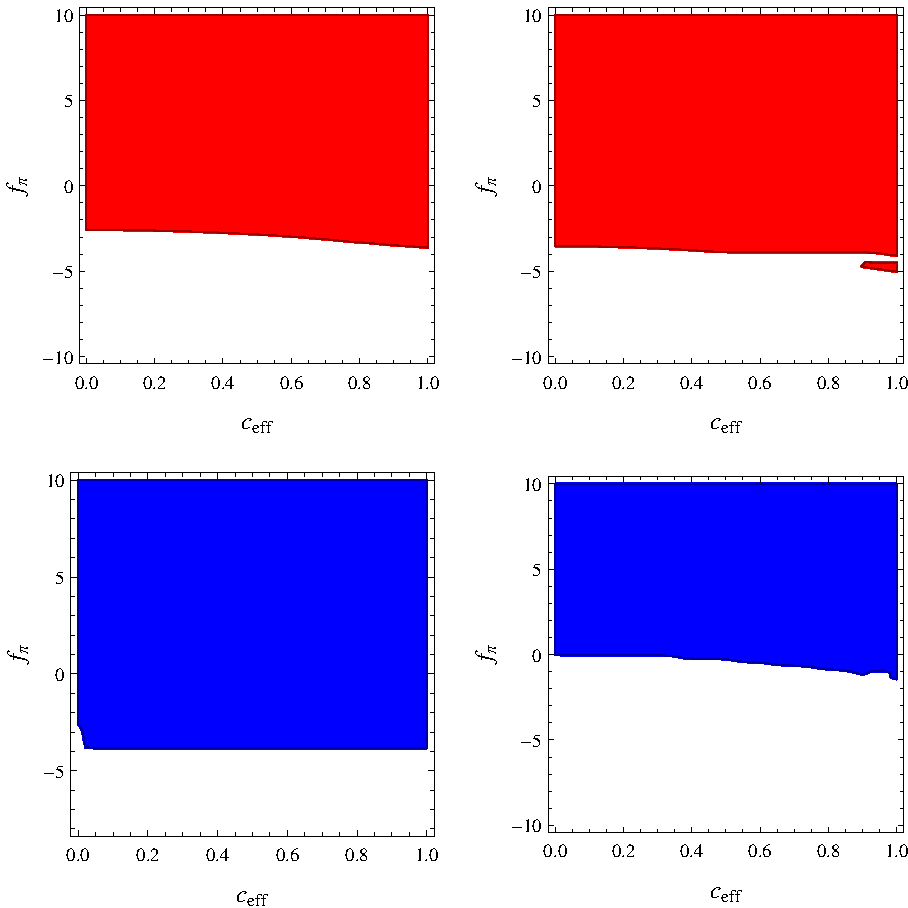
\includegraphics[width=\textwidth]{figures/chapter-ade/stability2.pdf} 
\caption{Stability regions: parameter regions where the perturbations grow more slowly than $a^2$ at $a=5\times10^{-2}$, for $w=-1.05$ and $\aa=0$. The upper row (red contours) are for $k=5 H_0$, while the lower row (blue contours) is for $k=300 H_0$. The right panels are for $ \gg = 10^{-5} $ and the left panels for $ \gg=10^5 $.}
\label{fig:stability:2}
\end{figure} 

\chapter{General solutions}
\label{appendix2-ade}

In Section \ref{chapter-ade:phenomenology} we study some limiting cases in the $ 4- $dimensional system (\ref{eq:de-cont})--(\ref{eq:de-eul}) for which dark matter and dark energy perturbations decouple from each other.  In this appendix we give some solutions which are a bit cumbersome to be written in the main body of the paper. 

On sub-horizon scales and during matter dominance, dark energy density perturbations are governed by Eq. (\ref{eq:pheno7}) whose full solution is

\bea
\label{eq:appendix:A1}
\delta_{de} & = & \(\frac{\ceff k}{\H}\)  \, a^{\alpha_8}\,\lcb A_5\,  J_{-\nu_5}\( \frac{2 \ceff k}{\H} \) + A_6\, J_{\nu_5}\( \frac{2 \ceff k}{\H} \) \rcb  \\  
&+& \aa \beta_6\, a^{\alpha_7} \( \frac{\ceff k}{\H} \)^{\alpha_6} \,  J_{\nu_5}\( \frac{2 \ceff k}{\H} \) \, \tilde{{}_1F_2} \( \nu_6\,;\, \alpha_6\,, \nu_7\, ; -\frac{k^2 \ceff^2}{\H^2} \)  \nonumber \\ 
& - & \aa \beta_7 a^{\alpha_7} \( \frac{\ceff k}{\H} \)^{\alpha_{9}} J_{-\nu_5}\(  \frac{2\ceff k}{\H} \) \tilde{{}_1F_2} \( \nu_8\,;\, \alpha_{9}\,, \nu_{9}\, ; -\frac{k^2 \ceff^2}{\H^2} \), \nonumber  
 \eea

\noindent where 

\bea 
\nu_5^2 & = & \frac{432\ceff^4 + 48\ff^2 + 72\ceff^2(-1+4\ff-6w) + 3(1+6w)^2}{12} \nonumber \\
 &-& \frac{8\ff(3+4\gg^2+ 18w)}{12}\,,\\
\nu_6 & = & -\frac{5}{4} -\ff + n + \frac{3w-\nu_5}{2}\,,
\eea

\bea
\nu_7 & = & \nu_6 + 1\,,\\
\nu_8 & = &  -\frac{5}{4} -\ff + n + \frac{3w+\nu_5}{2}\,,\\
\nu_9 & = & \nu_8 + 1\,,\\
\alpha_6 & = & 1 - \nu_5\,, \\
\alpha_7 & = & -2(1 +\ff) +3w +n\,,\\
\alpha_8 & = &  -\ff + \frac{3w}{2} - \frac{3}{4}\,, \\
\alpha_{9} & = & 1 + \nu_5\,,
\eea

\bea
\beta_6 & = & \frac{1}{24} \frac{\ceff^{-2-4\ff+6w} k^{-4\ff+6w} }{H_0^{2-4\ff+6w}}   \Omega_m^{-1+2\ff-3w} \pi \delta_0 \csc \( \pi \nu_5\) \nonumber \\
 & \times & \Gamma \( \alpha_6\) \Gamma \( \nu_6\) \Gamma \( \alpha_{9}\)\,, \\
\beta_7 & = & \frac{1}{24} \frac{\ceff^{-2-4\ff+6w} k^{-4\ff+6w} }{H_0^{2-4\ff+6w}}   \Omega_m^{-1+2\ff-3w} \pi \delta_0 \csc \( \pi \nu_5\) \nonumber \\
 & \times & \Gamma \( \alpha_6\) \Gamma \( \nu_9\) \Gamma \( \alpha_{9}\)\,, 
\eea

\noindent $ A_5$, $ A_6  $ are constants of integration and $ \tilde{{}_1F_2} $ stands for the regularized generalized hypergeometric function. The last two terms in Eq. (\ref{eq:appendix:A1}) are due to the external anisotropic stress.

On the other hand, for sub-sound horizon scales, during dark energy domination and without external contribution to the dark energy anisotropic stress ($\aa=0$), we find (by using Eq. (\ref{eq:pheno19})) for dark energy velocity perturbations
\begin{align}
\label{eq:appendix:A2}
V_{de} = & \frac{1}{2} \( \frac{x_3}{2} \)^{\frac{1-\alpha_4}{1+3w}} \Bigg\{\,
  \bigg[\, 6(c_s^2-w) + 1-\alpha_4 \,\bigg] \times
 \nonumber \\ 
 &\times \[ B_4 \, \Gamma\(\frac{2+3w-\alpha_4}{1+3w}\)   J_{-\nu_1}(x_3)   + A_4\, \Gamma\(\frac{3w+\alpha_4}{1+3w}\)  J_{\nu_1}(x_3) \] \nonumber \\
&+ \frac{x_3 (1+3w)}{4} \[ B_4\,\Gamma\(\frac{2+3w-\alpha_4}{1+3w}\) \[ J_{-1-\nu_1}(x_3) - J_{1-\nu_1}(x_3)  \]    \right.
\nonumber \\
&+ \left. A_4\, \Gamma\(\frac{3w+\alpha_4}{1+3w}\) \[ J_{-1+\nu_1}(x_3) - J_{1+\nu_1}(x_3) \]    \]       \,\Bigg\} \, , 
\end{align}
%
while for dark matter velocity perturbations 
%
\bea 
\label{eq:appendix:A3}
V_m & = & \frac{3 (1+2\ff)}{1+3w} 2^{-\frac{2-\alpha_4 + \nu_1 +3w(1+\nu_1)}{1+3w}} x_3^{-\frac{-1+\alpha_4+\nu_1+3w\nu_1}{1+3w}} \,\Bigg\{
A_4 \, x_3^{2\nu_1} \nonumber \\
& \times & \Gamma\(\frac{3w+\alpha_4}{1+3w}\) \Gamma\( \frac{2-\alpha_4 +3w(\nu_1 -1)+\nu_1}{2+6w} \)
\nonumber \\ 
&\times & {}_1F_2\( \lcb \frac{2-\alpha_4 + 3w(\nu_1-1) + \nu_1}{2+6w} \rcb,\, \right. \nonumber \\
& & \left. {} \lcb 1+\nu_1,\, \frac{4-\alpha_4+\nu_1+3w(1+\nu_1)}{2+6w}  \rcb,\, -\frac{1}{4}x_3^2  \)
 \nonumber \\
&+& B_4\, 4^{\nu_1}\, \Gamma\( \frac{2+3w-\alpha_4}{1+3w} \) \Gamma\(-\frac{-2+\alpha_4 + \nu_1 +3w(1+\nu_1)}{2+6w} \)
\nonumber \\
&\times & {}_1F_2\( \lcb \frac{2-\alpha_4 - 3w(\nu_1+1) - \nu_1}{2+6w} \rcb,\, \right. \nonumber \\
& & \left. {} \lcb 1-\nu_1,\, \frac{4-\alpha_4-\nu_1-3w(-1+\nu_1)}{2+6w}  \rcb,\, -\frac{1}{4}x_3^2  \)  \,\Bigg\}
 \, ,
\eea
%
where $ \alpha_4,\, \nu_1  $ and $ x_3 $ are given by Eq. (\ref{eq:pheno20}). By means of this solution we can easily find an expression for dark matter density perturbations by solving the differential equation 
\be
\delta_m' = \frac{V_m}{a} \,.
\label{eq:appendix:A4}
\ee

%\chapter{$H_0$ and the different anchor distances}
\label{appendix1-h0}

\section{Introduction}

We have seen in Section \ref{chapter-h0:Summary} that results including all the available distance anchors are robust against the statistical method utilised in the analysis. In order to better understand both the data sets and the results in our 'standard analysis' we investigate below the application of our method to different combination of distance anchors excluding one or two of them. Our preferred $H_0$ measurements from subsections \ref{Subsection:A-NGC4258}-\ref{Subsection-A-Combining-distance-anchors} are shown in Figure \ref{Fig:single-combined-anchor}. 

\begin{figure}[hbtp]
\centering
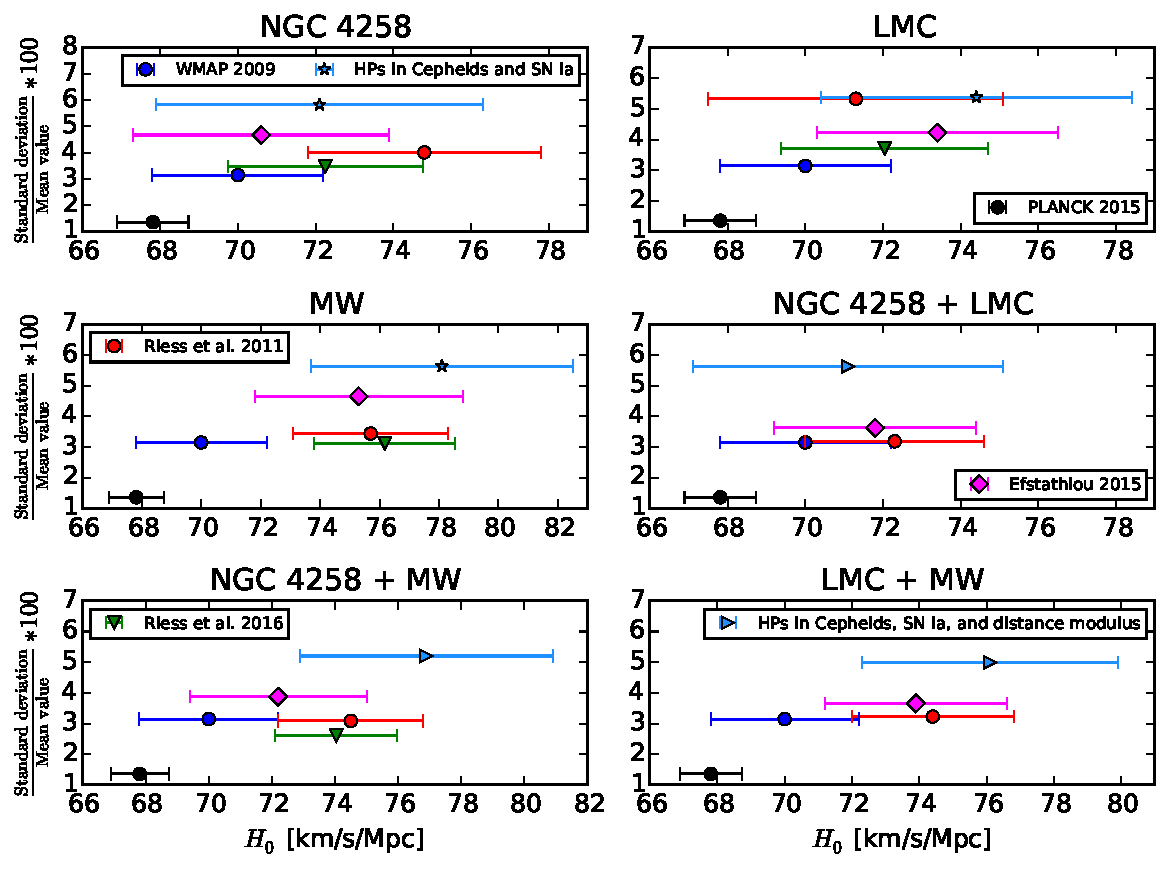
\includegraphics[scale=.8]{figures/chapter-h0/H0_values_anchor_combination.pdf}
\caption{Different measurements of the Hubble constant using different combinations of anchor distances. Colours and symbols are as in Figure \ref{Fig:H0-values-3-anchors}.}
\label{Fig:single-combined-anchor}
\end{figure}

\subsection{Megamaser system NGC 4258 distance modulus}
\label{Subsection:A-NGC4258}

In this subsection we apply our method to the sample of Cepheid variables and SNe Ia hosts in \cite{Riess:2011yx}, but restrict ourselves to a single anchor distance: the distance modulus to the megamaser system NGC 4258 from \cite{Humphreys:2013eja}. We include LMC Cepheid variables, but exclude MW Cepheid stars.  Results are shown in Table \ref{Table:NGC4258-fits}. We have explored two period cuts and two assumptions for the metallicity parameter $Z_W$.

The $H_0$ values in Table \ref{Table:NGC4258-fits} are shifted downwards w.r.t our 'standard analysis' value (Eq. \ref{Eq:H0-value-standard-analysis}) by $3-6 \%$. Fits with a tighter period cut prefer greater values of $H_0$: a $2\%$ change w.r.t those fits without period cut (independently of the metallicity dependence). Those changes are due to both $M_W-Z_W$ and $M_W-H_0$ degeneracies: a tighter period cut enhances metallicity dependence driving the Cepheid zero point to higher values which in turn prefers higher $H_0$. Allowing a metallicity dependence of the period-luminosity relation without prior on $Z_W$ we found a $>2\sigma$ departure from $Z_W=0$; This assumption, however, makes the Cepheid zero point $M_W$ less compatible with the value measured from MW Cepheid variables (see Eq. \eqref{Eq:MW-bestfit}). When HPs are used in Cepheid variables, SN Ia hosts, and distance modulus we obtain a $8\%$ measurement of the Hubble constant: the exclusion of two anchor distances in our 'standard analysis' makes the measurement more uncertain. Since for those fits the HP for the NGC 4258 distance modulus is always equal to one, we have also studied a couple of cases where only Cepheid variables and SNe Ia are included with HPs. As a result we obtain a $6\%$ measurement of $H_0$ which is still more uncertain than the corresponding case using the three anchor distances.

In the upper left panel of Figure \ref{Fig:single-combined-anchor} we show $H_0$ value from fit '$2^{ah}$' in Table \ref{Table:NGC4258-fits}, together with the values found by Riess et al. \cite{Riess:2011yx} ($H_0=74.8\pm 3.0 \, \km \second^{-1} \Mpc^{-1}$) which did not use the revised distance modulus from \cite{Humphreys:2013eja}, Efstathiou \cite{Efstathiou:2013via} ($H_0 = 70.6 \pm 3.3 \, \km \second^{-1} \Mpc^{-1}$), Riess et al. \cite{Riess:2016jrr} ($H_0=72.39\pm 2.56 \, \km \second^{-1} \Mpc^{-1}$) which used a redetermination of the distance modulus to NGC 4258. Our value is compatible with all previous direct determinations of $H_0$ and also with the indirect determinations from Planck and WMAP. The measurement using HPs is the most uncertain among the direct measurements due to inclusion of SNe Ia with HPs. The Planck collaboration used Efstathiou's value as a prior for $H_0$ when combining CMB measurements and local measurements of the Hubble constant. This assumption could lead to different conclusions in their analysis if another prior is utilised.

\begin{table}[tbp]
\centering
\begin{tabular}{@{}lccccr}
\hline
\multicolumn{6}{c}{NGC $4258$ anchor} \\
\hline
Fit & $H_0$ & $M_W$ & $b_W$ & $Z_W$ & $\sigma_{\intt}^{\LMC}$  \\
\hline
$1^a$ & $71.2\,(5.4)$& $-3.54\,(1.24)$ & $-3.15\,(0.06)\,[N]$ & $-0.285\,(0.140)\,[N]$ & $0.07$ \\
  
$1^b$ & $72.5\,(5.4)$& $-1.99\,(1.33)$ & $-3.25\,(0.05)\,[N]$ & $-0.457\,(0.150)\,[N]$ & $ 0.06$\\
   
$2^a$ & $71.1\,(5.5)$& $-6.00\,(0.22)$&$-3.17\,(0.06)\,[N]$ &$-0.006\,(0.020)\,[S]$ & $ 0.07$\\

$2^{ah}$ & $70.8\,(4.2)$& $-6.01\,(0.19)$&$-3.17\,(0.06)\,[N]$ &$-0.006\,(0.020)\,[S]$ & $ 0.07$\\

$2^b$ & $72.7\,(5.7)$& $-5.94\,(0.22)$&$-3.26\,(0.05)\,[N]$ &$-0.008\,(0.020)\,[S]$ & $ 0.06$\\

$2^{bh}$ & $72.1\,(4.2)$& $-5.95\,(0.19)$&$-3.26\,(0.05)\,[N]$ &$-0.008\,(0.020)\,[S]$ & $ 0.06$\\

\hline
\end{tabular}
\caption{\label{Table:NGC4258-fits} Numbers in brackets give the standard deviation. $[S]$ stands for the strong prior used in Subsection \ref{Subsection:combining-anchors}. SNe Ia hosts are included with HPs. Fits with superscript $^h$ include NGC 4258 distance modulus without HPs. For all the fits without superscript $^h$ the effective HP for the anchor is equal to one. Superscripts $^a$ and $^b$ indicate period cuts as in Table \ref{Table:LMC-fits}. For the SNe Ia hosts, $\sum_{i=1}^{8}  \alpha^{\eff,\,\SNe}_{i}$ ranges from $5.7$ (fits '$2^{ah}$' and '$2^a$') to $6.6$ (fit '$1^b$'). }
\end{table}


%\begin{table}[tbp]
%\centering
%\begin{tabular}{@{}lccccr}
%\hline
%\multicolumn{6}{c}{Distance parameters} \\
%\hline
%Host & SN Ia & $\mu_{0,i}-\mu_{0,4258}$ & $\mu_{0,i} $ best & $\alpha_{eff}$ & $\sigma_{int,i}^{R11}$\\
%\hline
%
% n4536 & SN 1981B & $1.619\,(0.0698)$&$31.04\,(0.12)$ &$1$ & $0.03$ \\
%
% n4639 & SN 1990N & $2.323\,(0.0844)$& $31.75\,(0.13)$& $1 $ & $0.01$\\
%
% n3370 & SN 1994ae & $2.502\,(0.0821)$& $31.93\,(0.13)$& $0.07 $ & $0.008$ \\
% 
% n3982 & SN 1998aq & $2.778\,(0.0656)$& $32.20\,(0.12)$& $ 0.04$ & $0.01$\\
%  
% n3021 & SN 1995al & $2.968\,(0.1080)$& $32.39\,(0.15)$& $ 0.6$ & $0.01$\\
%    
% n1309 & SN 2002fk & $3.229\,(0.0783)$& $32.65\,(0.13)$& $ 0.9$ & $0.01$\\
%
% n5584 & SN 2007af & $2.256\,(0.1009)$& $31.68\,(0.15)$& $ 0.09$ & $0.01$\\
%       
% n4038 & SN 2007sr & $2.379\,(0.0650)$& $31.80\,(0.12)$& $ 1$ & $0.01$\\
%       
%\hline
%\end{tabular}
%\caption{\label{Table:SNIa-NGC4258-fit-3} Numbers in brackets give the standard deviation on the parameters computed from the MCMC for fit $3^{ac}$ in Table \ref{Table:NGC4258-fits}. The last column gives the effective HP for each SN Ia.}
%\end{table}
%
%\begin{figure}[tbp]
%\centering % \begin{center}/\end{center} takes some additional vertical space
%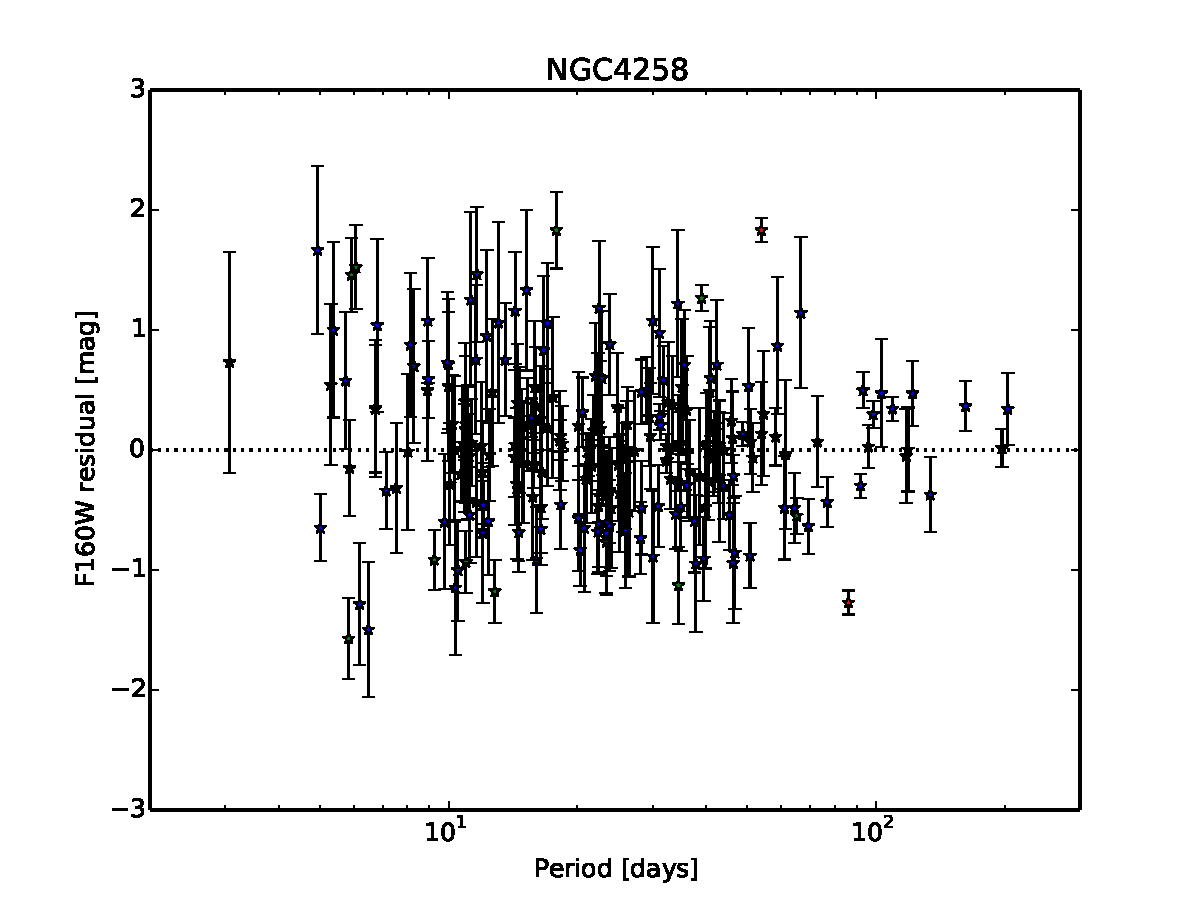
\includegraphics[scale=0.6]{effective_HP_F160W_cepheids_NGC4258.pdf}
%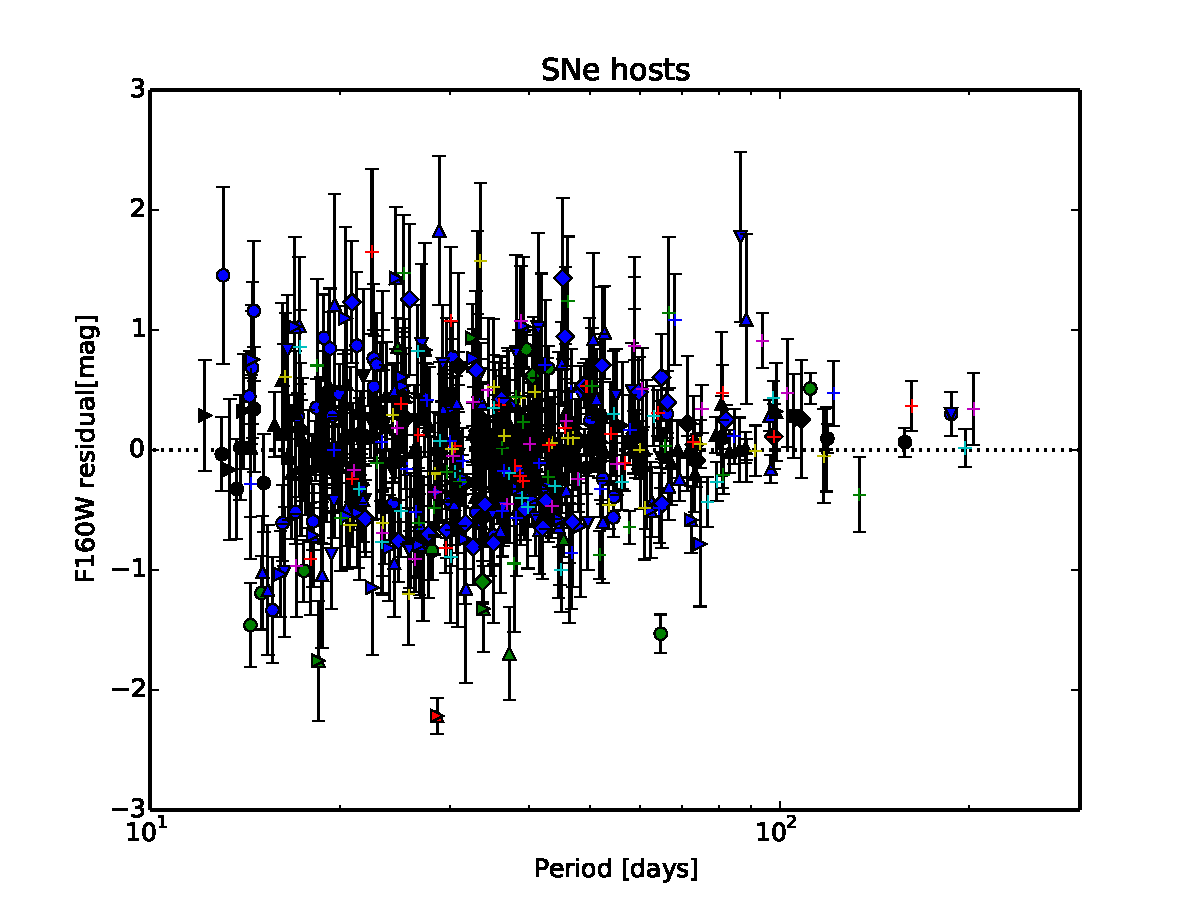
\includegraphics[scale=0.6]{effective_HP_F160W_cepheids_SNe.pdf} 
%\caption{Residuals for the P-L relation relative to global fit 3 in Table \ref{Table:NGC4258-fits}. Upper panel shows residuals for NGC4258 Cepheid variables and the SNe host galaxy Cepheid variables are shown in the bottom panel. Data points are colour-coded as in Figure \ref{Fig:LMC-Cepheid-variables-fit-c} corresponding to their HPs values. Error bars are not rescaled.}
%\label{Fig:Residuals-P-L-relation-fit-3}
%\end{figure}

\subsection{LMC distance modulus}
\label{Subsection:LMC-anchor}

In this subsection we apply our method to the sample of Cepheid variables and SNe Ia hosts in \cite{Riess:2011yx}, but restrict ourselves to a single anchor distance: the distance modulus to the LMC from \cite{Pietrzynski:2013gia}. We also include NGC4258 Cepheid variables, but omit MW Cepheid variables. Results are shown in Table \ref{Table:LMC-fits-anchor}. We have examined different period cuts and different assumptions for the metallicity dependence in the Leavitt Law.

The fits in Table \ref{Table:LMC-fits-anchor} show a $0-7\%$ shift in $H_0$ w.r.t the value in Eq. \eqref{Eq:H0-value-standard-analysis}. A period cut shifts $H_0$ values by $0.7-2\%$ (w.r.t. fits without period cut), whereas the use of HPs in LMC distance modulus changes $H_0$ values by $\lesssim 0.4\%$. In Figure \ref{Fig:constraints-fit-5a} we show $1-$D and $2-$D posteriors for fit '$5^a$'. Due to the $M_W-Z_W$, $M_W-H_0$, $Z_W-H_0$ degeneracies, $H_0$ is pushed towards higher values when a strong prior on the metallicity parameter $Z_W$ is utilised: the strong prior on $Z_W$ pushes $M_W$ to more negative values which in turn drives $H_0$ to higher values. When no prior on $Z_W$ is used along with a tighter cut period we observe a $3\sigma$ departure from $Z_W=0$. This, however, makes the Cepheid zero point $M_W$ less compatible with the value determined from MW Cepheid variables (Eq. \eqref{Eq:MW-bestfit}).

Fits in Table \ref{Table:LMC-fits-anchor} represent  $5-7\%$ measurements of the Hubble constant. In upper right panel of Figure \ref{Fig:single-combined-anchor} we show $H_0$ value of fit '$6^{ah}$' along with measurements by Riess et al. \cite{Riess:2011yx} ($H_0=71.3\pm 3.8 \, \km \second^{-1} \Mpc^{-1}$), Efstathiou \cite{Efstathiou:2013via} ($H_0 = 73.4 \pm 3.1 \, \km \second^{-1} \Mpc^{-1}$), Riess et al. \cite{Riess:2016jrr} ($H_0=71.93\pm 2.70 \, \km \second^{-1} \Mpc^{-1}$). Our measurement is almost as precise as that of \cite{Riess:2011yx} and is in good agreement with all the other direct determinations of the Hubble constant. While the WMAP value agrees at $1\sigma$ level with ours, the Planck value agrees at $2\sigma$ level.

\begin{table}[tbp]
\centering
\begin{tabular}{@{}lccccr}
\hline 
\multicolumn{6}{c}{LMC anchor} \\
\hline 
Fit & $H_0$ & $M_W$ & $b_W$ & $Z_W$ & $\sigma_{\intt}^{\LMC}$ \\
\hline
$5^a$ & $71.3\,(4.9)$& $-3.48\,(1.16)$ & $-3.15\,(0.06)\,[N]$& $-0.291\,(0.136)\,[N]$ & $0.07$ \\
 
$5^b$ & $70.1\,(4.5)$& $-2.11\,(1.28)$ & $-3.26\,(0.05)\,[N]$& $-0.450\,(0.150)\,[N]$ & $ 0.06$ \\	
  
$6^a$ & $74.5\,(4.9)$& $-5.90\,(0.20)$& $-3.17\,(0.06)\,[N]$& $-0.006\,(0.020)\,[S]$ & $0.07$ \\

$6^{ah}$ & $74.4\,(4.0)$& $-5.90\,(0.18)$& $-3.17\,(0.06)\,[N]$& $-0.006\,(0.020)\,[S]$& $0.07$ \\

$6^b$ & $75.0\,(4.8)$& $-5.87\,(0.20)$& $-3.26\,(0.05)\,[N]$& $-0.008\,(0.020)\,[S]$ & $ 0.06$ \\
   
$6^{bh}$ & $74.7\,(3.8)$& $-5.87\,(0.18)$& $-3.26\,(0.05)\,[N]$& $-0.008\,(0.020)\,[S]$& $ 0.06$ \\
   
\hline   
\end{tabular}
\caption{\label{Table:LMC-fits-anchor} Numbers in brackets give the standard deviation. $[S]$ stands for the strong prior used in Subsection \ref{Subsection:combining-anchors}. SNe Ia hosts are included with HPs. Fits with superscript $^h$ include LMC distance modulus without HPs. For all the fits without superscript $^h$ the effective HP for the anchor is equal to one. Superscripts $^a$ and $^b$ indicate period cuts as in Table \ref{Table:LMC-fits}. For SNe Ia hosts, $\sum_{i=1}^{8}  \alpha^{\eff,\,\SNe}_{i}$ ranges from $5.9$ (fit '$6^{bh}$') to $7$ (fit '$5^b$').}
\end{table}

\begin{figure}[hbtp]
\centering
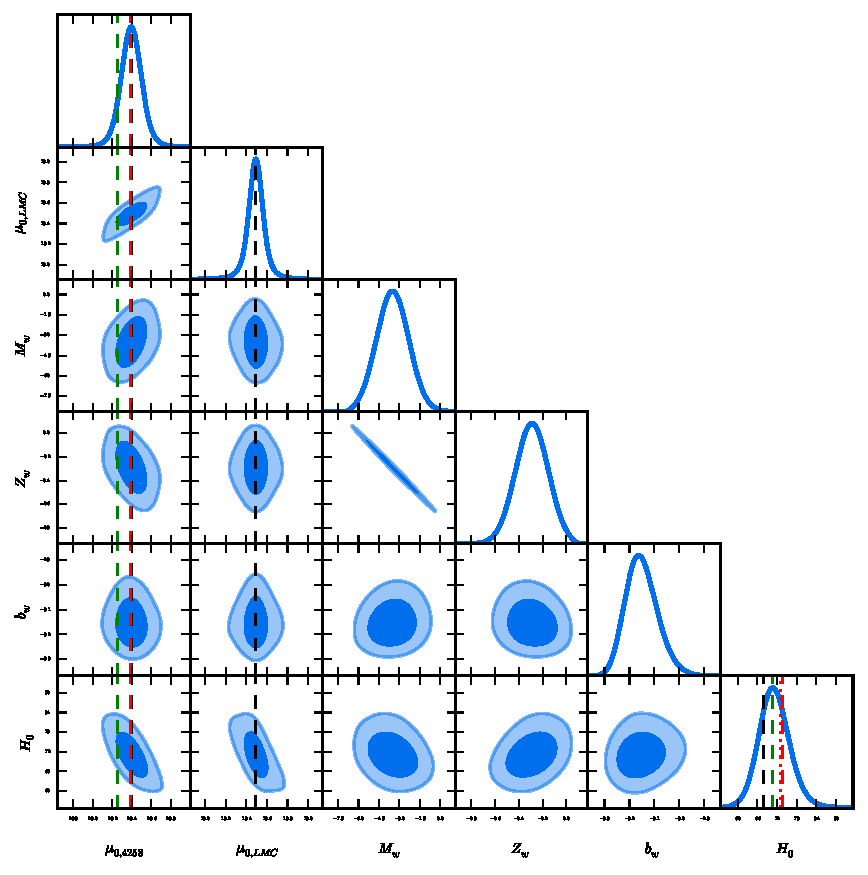
\includegraphics[scale=1]{figures/chapter-h0/triangle_figure_fit_5a.pdf}
\caption{Posterior constraints for fit '$5^a$'. Vertical lines show measurements of $\mu_{0,4258}$, $\mu_{0,\LMC}$, and $H_0$ as indicated in caption of Figure \ref{Fig:Main-analysis-fitM1a}.  \label{Fig:constraints-fit-5a}}
\end{figure}

\subsection{Parallax measurements of Cepheid variables in the Milky Way}
\label{Subsection:MW}

Parallax measurements of Cepheid variables (see Subsection \ref{Subsection:MW-1}) in our galaxy are used in this Section as the sole anchor distance scale. We include Cepheid variables in both the megamaser system NGC 4258 and those in the LMC. We show the resulting constraints in Table \ref{Table:MW-fits}. In addition to different period cuts and different assumptions for the metallicity dependence in the Leavitt Law, we have included some cases where those hosts galaxies whose slope $b_W$ departs from the LMC value (fit 'c' in Table \ref{Table:LMC-fits}) by $\gtrsim 2\sigma$ are excluded from the fit.

All fits in Table \ref{Table:MW-fits} including the whole data set are shifted upwards w.r.t our 'standard analysis' by $3-4\%$. In this case we obtain a $5-6\%$ measurement of the Hubble constant. A tighter period cut in the Leavitt Law shifts $H_0$ values by $0.3-0.4\%$ (w.r.t. fits without period cut). A strong prior on the metallicity parameter $Z_W$ drives downwards $H_0$ by $1-2\%$ (w.r.t. fits with no prior). When including the metallicity dependence without a prior we observe a slight $b_W-H_0$ degeneracy: less negative $b_W$ prefers higher $H_0$ values. Fits with a superscript $^l$ do not include Cepheid variables in galaxy hosts with a slope $b_W$ differing $\gtrsim 2\sigma$ from the LMC value. The main impact of this change is seen in $H_0$ having both mean value and standard deviation increased. Furthermore, those cases without prior on $Z_W$ present an enhancement on their metallicity dependence. As expected the slope $b_W$ is now closer to the LMC value (even without a tighter period cut).

In the middle left panel of Figure \ref{Fig:single-combined-anchor} we show $H_0$ value from fit $10^b$ along with values determined by Riess et al. \cite{Riess:2011yx} ($H_0=75.7\pm 2.6 \, \km \second^{-1} \Mpc^{-1}$); Efstathiou  \cite{Efstathiou:2013via} ($H_0 = 75.3 \pm 3.5 \, \km \second^{-1} \Mpc^{-1}$); Riess et al. \cite{Riess:2016jrr} ($H_0=76.09\pm 2.41 \, \km \second^{-1} \Mpc^{-1}$) that used a bigger sample of MW Cepheid variables. Our measurement is the most uncertain, but it is compatible with all other direct measurements showing that the value is robust against the statistical approach employed. All direct measurements present a $\approx 2\sigma$ disagreement with the Planck value.

\begin{table}[tbp]
\centering
\begin{tabular}{@{}lcccccr}
\hline 
\multicolumn{7}{c}{Milky Way anchor} \\
\hline 
Fit & $H_0$ & $M_W$ & $b_W$ & $Z_W$ & $\sigma_{\intt}^{\MW}$ & $\sigma_{\intt}^{\LMC}$ \\
\hline
$9^a$ & $78.1\,(4.4)$& $-3.44\,(1.25)$ & $-3.16\,(0.06)\,[N]$& $-0.272\,(0.140)\,[N]$ & $ 0.02 $ & $0.07$ \\

$9^{al}$ & $83.9\,(9.7)$& $-2.00\,(1.60)$ & $-3.27\,(0.05)\,[N]$& $-0.436\,(0.179)\,[N]$ & $ 0.02$ & $0.06$ \\
 
$9^b$ & $78.3\,(4.2)$& $-2.08\,(1.19)$ & $-3.26\,(0.05)\,[N]$& $-0.426\,(0.133)\,[N]$ & $0.02$ & $0.06$\\

$9^{bl}$ & $84.6\,(9.5)$& $-1.56\,(1.66)$ & $-3.27\,(0.05)\,[N]$& $-0.485\,(0.186)\,[N]$ & $0.02$ & $0.06$\\
  
$10^a$ & $77.4\,(4.4)$& $-5.81\,(0.18)$& $-3.17\,(0.06)\,[N]$& $-0.006\,(0.020)\,[S]$ & $0.02$ & $0.07$ \\

$10^{al}$ & $80.9\,(8.3)$& $-5.83\,(0.19)$& $-3.28\,(0.05)\,[N]$& $-0.007\,(0.020)\,[S]$ & $0.02$ & $0.06$ \\

$10^b$ & $77.1\,(4.1)$& $-5.81\,(0.18)$& $-3.26\,(0.05)\,[N]$& $-0.008\,(0.020)\,[S]$ & $0.02 $ & $0.06$ \\
   
$10^{bl}$ & $80.7\,(8.2)$& $-5.83\,(0.18)$& $-3.28\,(0.05)\,[N]$& $-0.006\,(0.020)\,[S]$ & $0.02 $ & $0.06$ \\
   
\hline   
\end{tabular}
\caption{\label{Table:MW-fits} For the MW Cepheid variables we find that $\sum_{i=1}^{13} \alpha^{\eff,\,\MW}_{i}$ ranges between $11.5$ (fit $9^a$) and $12$ (fit $10^b$). For the SNe Ia hosts the fit gives $\sum_{i=1}^{8} \alpha^{\eff,\,\SNe}_{i}$ ranging from $5.1$ (fit $10^a$) to $6.5$ (fit $9^a$).}
\end{table}

\subsection{Combining two distance anchors}
\label{Subsection-A-Combining-distance-anchors}

It is difficult to argue for specific choices of distance anchors, which is why we decided to combine all
anchors in the main text. Here we provide the constraints for different combinations of two anchor distances. Results are shown in Tables \ref{Table:Joint-Constraints-NGC-LMC}-\ref{Table:Joint-Constraints-LMC-MW}. 

Using distance moduli to both NGC 4258 and LMC as anchor distances we see that the effect of the strong prior on the metallicity parameter is less important than in the case where only LMC is utilised as anchor distance. There is also a $\approx 2\sigma$ departure from $Z_W=0$ when no prior on $Z_W$ is used, but the Cepheid zero point is is disagreement with the value measured by MW Cepheid variables alone. As noted before for the case using only LMC as anchor distance, again here the $M_W-H_0$, $M_W-Z_W$, and $Z_W-H_0$ degeneracies drive $H_0$ towards higher values. The change, however, is smaller than in the case where only LMC is used as anchor. In the middle right panel of Figure \ref{Fig:single-combined-anchor} we show $H_0$ value from fit '$14^b$' as well as the measurements of Riess et al. ($H_0=72.3\pm 2.3 \, \km \second^{-1} \Mpc^{-1}$) \cite{Riess:2011yx} and Efstathiou ($H_0=71.8\pm 2.6 \, \km \second^{-1} \Mpc^{-1}$) \cite{Efstathiou:2013via}.

Fits including both distance modulus to NGC 4258 and MW Cepheid variables as distance anchors follow same trend as fits only including MW Cepheid variables as distance anchor: $H_0$ is pushed downwards when a strong prior on the metallicity parameter is used, and the period cut does not have a big impact on the $H_0$ value. In the lower left panel of Figure \ref{Fig:single-combined-anchor} we show $H_0$ value from fit '$17^b$' as well as the measurements of Riess et al. ($H_0=74.5\pm 2.3 \, \km \second^{-1} \Mpc^{-1}$) \cite{Riess:2011yx}, Efstathiou ($H_0=72.2\pm 2.8 \, \km \second^{-1} \Mpc^{-1}$) \cite{Efstathiou:2013via}, and Riess et al ($H_0=73.85\pm 1.97 \, \km \second^{-1} \Mpc^{-1}$) \cite{Riess:2016jrr}.

Fits including both MW Cepheid variables and LMC distance modulus as anchor distances also follow same trend as for the case where MW Cepheid variables are used as the only anchor distance. In the lower right panel of Figure \ref{Fig:single-combined-anchor} we show measurement of fit '$22^b$' along with measurements by Riess et al. ($H_0=74.4\pm 2.4 \, \km \second^{-1} \Mpc^{-1}$) \cite{Riess:2011yx}, and Efstathiou ($H_0=73.9\pm 2.7 \, \km \second^{-1} \Mpc^{-1}$) \cite{Efstathiou:2013via}.
 
\begin{table}[tbp]
\centering
\begin{tabular}{@{}lccccr}
\hline
\multicolumn{6}{c}{NGC $4258\,+$ LMC anchors} \\
\hline
Fit & $H_0$ & $M_W$ & $b_W$ & $Z_W$  &$\sigma_{\intt}^{\LMC}$ \\
\hline 
$13^a$ &$ 71.1\,(4.0)$ & $-3.47\,(1.10)$& $-3.15\,(0.06)\,[N]$& $-0.293\,(0.128)\,[N]$ & $0.07$ \\

$13^b$ &$ 71.2\,(4.0)$ & $-2.27\,(1.16)$& $-3.25\,(0.05)\,[N]$& $-0.428\,(0.135)\,[N]$ & $0.06$ \\

$14^a$ &$73.0\,(4.1)$ & $-5.93\,(0.18)$& $-3.17\,(0.06)\,[N]$& $-0.007\,(0.020)\,[S]$ & $0.07$ \\

$14^b$ &$73.9\,(4.0)$ & $-5.89\,(0.18)$& $-3.26\,(0.05)\,[N]$& $-0.008\,(0.020)\,[S]$ & $0.06$ \\
\hline  
\end{tabular}
\caption{Distance modulus to both NGC 4258 and LMC are included with HPs. $\alpha_{\LMC}^{\eff}=\alpha_{4258}^{\eff}=1$ for all the fits except for the fit '$14^a$' where $\alpha_{4258}^{\eff}=0.7$. For the SNe Ia hosts the fits give $\sum_{i=1}^{8} \alpha^{\eff,\,\SNe}_{i}$ ranging from $5.4$ (fit $13^b$) to $6.5$ (fit $13^a$). \label{Table:Joint-Constraints-NGC-LMC} }
\end{table}

\begin{table}[tbp]
\centering
\begin{tabular}{@{}lcccccr}
\hline 
\multicolumn{7}{c}{NGC $4258\, +$ MW anchors} \\
\hline
Fit & $H_0$ & $M_W$ & $b_W$ & $Z_W$ &$\sigma_{\intt}^{\MW}$ & $\sigma_{\intt}^{\LMC}$ \\
\hline 
$17^a$ & $76.4\,(4.2)$&$-3.44\,(1.27)$ &$-3.18\,(0.06)\,[N]$ &$-0.277\,(0.142)\,[N]$ & $0.02$& $0.07$\\
 
$17^b$ & $76.9\,(4.0)$&$-2.13\,(1.27)$ &$-3.27\,(0.04)\,[N]$ &$-0.425\,(0.143)\,[N]$ & $0.01$& $0.06$\\
 
$18^a$ &$75.6\,(4.2)$ &$-5.85\,(0.18)$ &$-3.20\,(0.05)\,[N]$ &$-0.006\,(0.020)\,[S]$ &$0.02$ & $0.06$\\

$18^b$ &$75.8\,(3.9)$ &$-5.84\,(0.18)$ &$-3.27\,(0.04)\,[N]$ &$-0.008\,(0.020)\,[S]$ &$0.02$ & $0.06$\\
\hline  
\end{tabular}
\caption{Distance modulus to the megamaser system NGC 4258 is included with HPs. All the fits have $\alpha_{4258}^{\eff}<1$, values ranging from $0.2$ (fit '$17^a$') to $0.5$ (fit '$17^b$'). For the SNe Ia hosts the fits give $\sum_{i=1}^{8} \alpha^{\eff,\,\SNe}_{i}$ ranging from $5.6$ (fit $17^b$) to $6.4$ (fit $17^a$) \label{Table:Joint-Constraints-NGC-MW} }
\end{table}

\begin{table}[tbp]
\centering
\begin{tabular}{@{}lcccccr}
\hline
\multicolumn{7}{c}{LMC $+$ MW anchors} \\
\hline
Fit & $H_0$ & $M_W$ & $b_W$ & $Z_W$ &$\sigma_{\intt}^{\LMC}$ & $\sigma_{\intt}^{\MW}$ \\
\hline 
$21^a$ & $76.0\,(4.2)$ &$-4.33\,(1.16)$ &$-3.18\,(0.06)\,[N]$ &$-0.178\,(0.131)\,[N]$ & $0.07$& $0.02$\\

$21^b$ & $76.2\,(4.1)$ &$-3.10\,(1.31)$ &$-3.27\,(0.05)\,[N]$ &$-0.318\,(0.147)\,[N]$ & $0.06$& $0.02$\\
 
$22^a$ &$76.0\,(4.0)$ &$-5.86\,(0.18)$ &$-3.19\,(0.05)\,[N]$ &$-0.004\,(0.020)\,[S]$ & $0.06$ & $0.02$\\

$22^b$ &$76.1\,(3.8)$ &$-5.84\,(0.18)$ &$-3.27\,(0.04)\,[N]$ &$-0.007\,(0.020)\,[S]$ &$0.06$ & $0.02$\\
\hline 
\end{tabular}
\caption{Both SNe Ia and distance modulus to LMC are included with HPs. Fit '$22^b$' is the only one for which the distance modulus to LMC is not down-weighted; Values for the others fits range from $0.1$ (fits '$21^a$' and '$21^b$') to $0.6$ (fit '$22^a$'). For the SNe Ia hosts the fits give $\sum_{i=1}^{8} \alpha^{\eff,\,\SNe}_{i}$ ranging from $5.7$ (fit $22^b$) to $6.6$ (fit $22^b$). The sum of effective HPs for MW Cepheid variables ranges from $11.7$ (fits '$21^b$' and '$22^b$') to $12.1$ (fit '$21^a$').\label{Table:Joint-Constraints-LMC-MW}}
\end{table}
%\begin{tabular}{@{}lcccccr}
%\hline 
%\multicolumn{7}{c}{NGC $4258 +$ LMC $+$ MW anchors} \\
%\hline
%Fit & $H_0$ & $M_W$ & $b_W$ & $Z_W$ &$\sigma_{\intt}^{\LMC}$ & $\sigma_{\intt}^{\MW}$ \\
%\hline 
%$25^a$ & $74.8\,(4.0)$&$-4.33\,(1.10)$ &$-3.19\,(0.05)\,[N]$ &$-0.180\,(0.124)\,[N]$ & $0.06$& $0.009$& $0.03$ \\

%$25^b$ & $75.1\,(3.9)$&$-3.19\,(1.24)$ &$-3.28\,(0.04)\,[N]$ &$-0.310\,(0.140)\,[N]$ & $0.06$& $0.009$& $0.01$ \\

%$26^a$ & $74.6\,(3.9)$&$-5.88\,(0.18)$ &$-3.19\,(0.05)\,[N]$ &$-0.005\,(0.020)\,[Y]$ & $0.06$& $0.011$& $0.04$\\

%$26^b$ & $75.5\,(3.9)$&$-5.86\,(0.18)$ &$-3.27\,(0.04)\,[N]$ &$-0.007\,(0.020)\,[Y]$ & $0.06$& $0.008$& $0.01$\\

%$27^a$ & $75.2\,(3.9)$&$-5.86\,(0.18)$ &$-3.22\,(0.04)\,[Y]$ &$-0.004\,(0.020)\,[Y]$ & $0.06$& $0.009$& $0.03$\\

%$27^b$ & $75.9\,(3.8)$&$-5.84\,(0.18)$ &$-3.28\,(0.04)\,[Y]$ &$-0.006\,(0.020)\,[Y]$ & $0.05$& $0.009$& $0.01$\\

%$28^a$ & $75.0\,(4.0)$&$-4.47\,(1.13)$ &$-3.22\,(0.04)\,[Y]$ &$-0.162\,(0.127)\,[N]$ &$0.06$ &$0.009$ & $0.03$\\
  
%$28^b$ & $75.9\,(4.0)$&$-3.22\,(1.29)$ &$-3.28\,(0.04)\,[Y]$ &$-0.304\,(0.145)\,[N]$ & $0.05$& $0.009$& $0.01$\\
  
%\hline 
%\end{tabular}


%\subsection{Previous Results}
%\label{Section:Results}
%
%Table \ref{Table:Constraints} shows previous results with fixed $\sigma_{\rm int}$. \commentr{Constraints on relevant parameters. Fits with $\star$ include anchors with HPs and those with $\diamond$ include HPs in SNIa.$\heartsuit$ includes HPs in metallicity. $\square$ includes MW dataset with a HP with Jeffrey's prior.}
%
%\begin{table}[tbp]
%\centering
%\begin{tabular}{@{}lcccccccr}
%\hline
%\multicolumn{9}{c}{NGC $4258$ anchor} \\
%\hline
%Fit & $H_0$ & $zp_W$ & $b_W$ & $Z_W$ & $\sigma_{int}$ & Prior $Z_W$ & Prior $b_W$  & P \\
%\hline
% A1 & $70.5\,(3.1)$& $26.34\,(0.26)$ & $-3.00\,(0.13)$ & $-0.008\,(0.020)$& $0.14$ & S & N & $60$ \\
%  
% A2 & $71.2\,(3.3)$& $26.32\,(0.26)$&$-2.99\,(0.14)$ &$-0.007\,(0.020)$ & $0.2$ & S & N & $60$ \\
%
% A3 & $70.3\,(2.9)$& $26.12\,(0.22)$& $-2.86\,(0.09)$& $-0.006\,(0.020)$& $0.2$ & S & N & $205$ \\
% 
%\end{tabular}
%\begin{tabular}{@{}lcccccccr}
%\hline 
%\multicolumn{9}{c}{LMC anchor} \\
%\hline 
%Fit & $H_0$ & $zp_W$ & $b_W$ & $Z_W$ & $\sigma_{int}$ & Prior $Z_W$ & Prior $b_W$  & P \\
%\hline
% A4 & $70.0\,(2.5)$& $19.35\,(1.31)$ & $-3.19\,(0.07)$& $-0.43\,(0.15)$& $0.14$ & N & N & $60$ \\
% 
% A5 & $70.2\,(2.9)$& $19.30\,(1.42)$& $-3.19\,(0.07)$& $-0.42\,(0.17)$& $0.2$ & N & N & $60$ \\
% 
% A6 & $70.4\,(2.0)$& $18.36\,(1.20)$ & $-3.07\,(0.07)$& $-0.32\,(0.14)$& $0.2$ & N & N & $205$ \\
% 
% A7 & $73.9\,(2.6)$& $15.80\,(0.19)$ & $-3.20\,(0.07)$& $-0.006\,(0.020)$& $0.14$ & S & N & $60$ \\
% 
% A8 & $72.8\,(2.3)$& $15.82\,(0.19)$& $-3.22\,(0.07)$& $-0.006\,(0.020)$& $0.2$ & S & N & $60$ \\
% 
% A9 & $73.9\,(2.7)$& $15.66\,(0.19)$ & $-3.09\,(0.07)$& $-0.005\,(0.020)$& $0.2$ & S & N & $205$ \\
%   
%\end{tabular}
%\begin{tabular}{@{}lcccccccr}
%\hline
%\multicolumn{9}{c}{MW anchor} \\
%\hline 
%Fit & $H_0$ & $M_W$ & $b_W$ & $Z_W$ & $\sigma_{int}$ & Prior $Z_W$ & Prior $b_W$  & P \\
%\hline
%A10 & $81.5\,(4.5)$& $-5.74\,(0.19)$& $-3.06\,(0.12)$ & $-0.007\,(0.020)$ & $0.14$ & S & N & $60$ \\
% 
%A11 &$80.1\,(4.7)$ & $-5.76\,(0.19)$ &$-3.09\,(0.13)$ & $-0.006\,(0.020)$& $0.2$ & S & N & $60$ \\
% 
%A12 & $85.0\,(4.2)$ & $-5.72\,(0.19)$ &$-2.90\,(0.09)$ & $-0.006\,(0.020)$& $0.2$ & S & N & $205$ \\
% 
%\end{tabular}
%\begin{tabular}{@{}lcccccccr}
%\hline
%\multicolumn{9}{c}{NGC $4258+$ LMC anchors} \\
%\hline
%Fit & $H_0$ & $M_W$ & $b_W$ & $Z_W$ & $\sigma_{int}$ & Prior $Z_W$ & Prior $b_W$  & P \\
%\hline 
%A13 &$72.6\,(1.7)$ & $-5.90\,(0.17)$& $-3.21\,(0.07)$& $-0.008\,(0.020)$& $0.14$ & S & N & $60$ \\
%
%A13$\heartsuit$ &$72.6\,(2.8)$ & $-5.66\,(0.42)$& $-3.21\,(0.07)$& $-0.037\,(0.049)$& $0.14$ & S & N & $60$ \\
% 
%A14 & $72.1\,(2.4)$ & $-5.91\,(0.18)$&$-3.22\,(0.07)$ &$-0.008\,(0.020)$ & $0.2$ & S & N & $60$ \\
%
%A14$\star$ & $72.1\,(2.9)$ & $-5.92\,(0.19)$ & $-3.21\,(0.07)$ & $-0.007\,(0.020)$ & $0.2$ & S & N & $60$ \\
%
%A14$\diamond$ & $74.1\,(3.9)$ & $-5.91\,(0.18)$ & $-3.22\,(0.07)$ & $-0.007\,(0.020)$ & $0.2$ & S & N & $60$ \\
% 
%A14$\star\diamond$ & $74.2\,(4.1)$ & $-5.93\,(0.18)$ & $-3.22\,(0.07)$ & $-0.006\,(0.020)$ & $0.2$ & S & N & $60$ \\
% 
%A15 &$72.3\,(2.4)$ &$-5.94\,(0.18)$ &$-3.10\,(0.07)$ &$-0.007\,(0.020)$ & $0.2$ & S & N & $205$ \\
% 
%A15$\star$ & $72.3\,(3.0)$ & $-5.96\,(0.19)$ & $-3.10\,(0.07)$ & $-0.006\,(0.020)$ & $0.2$ & S & N & $205$ \\
% 
%\end{tabular}
%\begin{tabular}{@{}lcccccccr}
%\hline 
%\multicolumn{9}{c}{NGC $4258 +$ MW anchors} \\
%\hline
%Fit & $H_0$ & $M_W$ & $b_W$ & $Z_W$ & $\sigma_{int}$ & Prior $Z_W$ & Prior $b_W$  & P \\
%\hline 
%A16 & $74.1\,(3.0)$&$-5.87\,(0.18)$ &$-3.21\,(0.10)$ &$-0.006\,(0.020)$ & $0.14$ & S & N & $60$ \\
% 
%A17 &$74.8\,(2.8)$ &$-5.85\,(0.18)$ &$-3.21\,(0.11)$ &$-0.007\,(0.019)$ & $0.2$ & S & N & $60$ \\
% 
%A18 &$76.1\,(3.0)$ &$-5.90\,(0.19)$ &$-3.03\,(0.08)$ &$-0.005\,(0.020)$ & $0.2$ & S & N & $205$ \\
% 
%\end{tabular}
%\begin{tabular}{@{}lcccccccr}
%\hline
%\multicolumn{9}{c}{LMC $+$ MW anchors} \\
%\hline
%Fit & $H_0$ & $M_W$ & $b_W$ & $Z_W$ & $\sigma_{int}$ & Prior $Z_W$ & Prior $b_W$  & P \\
%\hline 
%A19 & $74.7\,(2.5)$ &$-5.86\,(0.18)$ &$-3.23\,(0.07)$ &$-0.005\,(0.020)$ & $0.14$ & S & N & $60$ \\
% 
%A20 &$74.7\,(2.5)$ &$-5.86\,(0.18)$ &$-3.24\,(0.07)$ &$-0.004\,(0.020)$ & $0.2$ & S & N & $60$ \\
% 
%A21 &$75.2\,(2.6)$ &$-5.89\,(0.18)$ &$-3.13\,(0.06)$ &$-0.002\,(0.020)$ & $0.2$ & S & N & $205$ \\
% 
%\end{tabular}
%\begin{tabular}{@{}lcccccccr}
%\hline 
%\multicolumn{9}{c}{NGC $4258 +$ LMC $+$ MW anchors} \\
%\hline
%Fit & $H_0$ & $M_W$ & $b_W$ & $Z_W$ & $\sigma_{int}$ & Prior $Z_W$ & Prior $b_W$  & P \\
%\hline 
%A22 & $72.3\,(2.1)$&$-5.89\,(0.17)$ &$-3.27\,(0.06)$ &$-0.006\,(0.020)$ & $0.14$ & S & N & $60$ \\
%
%A22$\star$ & $73.9\,(2.6)$&$-5.86\,(0.18)$ &$-3.25\,(0.07)$ &$-0.006\,(0.020)$ & $0.14$ & S & N & $60$ \\
%
%A22$\diamond$ & $75.4\,(3.2)$&$-5.88\,(0.18)$ &$-3.26\,(0.06)$ &$-0.005\,(0.020)$ & $0.14$ & S & N & $60$ \\
%
%A22$\star \diamond$ & $76.4\,(3.8)$&$-5.86\,(0.18)$ &$-3.25\,(0.07)$ &$-0.006\,(0.020)$ & $0.14$ & S & N & $60$ \\
% 
%A23 & $72.5\,(2.6)$&$-5.88\,(0.18)$ &$-3.27\,(0.07)$ &$-0.006\,(0.020)$ & $0.2$ & S & N & $60$ \\
% 
%A23$\star$ & $73.9\,(2.7)$&$-5.87\,(0.18)$ &$-3.25\,(0.07)$ &$-0.005\,(0.020)$ & $0.2$ & S & N & $60$ \\
%
%A23$\diamond$ & $74.0\,(2.1)$&$-5.89\,(0.18)$ &$-3.27\,(0.06)$ &$-0.005\,(0.020)$ & $0.2$ & S & N & $60$ \\
%
%A23$\star \diamond$ & $76.4\,(3.4)$&$-5.86\,(0.18)$ &$-3.25\,(0.07)$ &$-0.005\,(0.020)$ & $0.2$ & S & N & $60$ \\
% 
%A23$\square$ & $73.6\,(2.3)$&$-5.86\,(0.18)$ &$-3.30\,(0.06)$ &$-0.004\,(0.020)$ & $0.2$ & S & N & $60$ \\
% 
%A24 &$71.2\,(1.4)$ &$-5.91\,(0.18)$ &$-3.18\,(0.06)$ &$-0.005\,(0.020)$ & $0.2$ & S & N & $205$ \\
% 
%A24$\star$ &$74.7\,(2.8)$ &$-5.88\,(0.18)$ &$-3.14\,(0.06)$ &$-0.003\,(0.020)$ & $0.2$ & S & N & $205$ \\
%
%A24$\diamond$ &$75.1\,(3.9)$ &$-5.91\,(0.18)$ &$-3.16\,(0.06)$ &$-0.004\,(0.020)$ & $0.2$ & S & N & $205$ \\
%
%A24$\star \diamond$ &$76.5\,(4.2)$ &$-5.88\,(0.18)$ &$-3.15\,(0.06)$ &$-0.003\,(0.020)$ & $0.2$ & S & N & $205$ \\
% 
% 
%\hline 
%\end{tabular}
%\caption{\label{Table:Constraints} Constraints on relevant parameters. Fits with $\star$ include anchors with HPs and those with $\diamond$ include HPs in SNIa.$\heartsuit$ includes HPs in metallicity. $\square$ includes MW dataset with a HP with Jeffrey's prior.}
%\end{table}


%\begin{figure}[tbp]
%\centering % \begin{center}/\end{center} takes some additional vertical space
%\includegraphics[scale=0.75]{effective_HP_cepheids_Efstathiou.pdf} 
%\caption{P-L magnitude residuals relative to  Plot with hyper-parameters and data points.}
%\label{Fig:hyper-parameters-and-data}
%\end{figure}


%\begin{figure}
%
%\caption{\label{Fig:H0-posteior} Posterior of $H_0$ when adding different terms and data.}
%\end{figure}


%\chapter{The Euclid photometric survey}
\label{appendix1-mnu}

Angular power spectra, depending on two redshifts $z_i$ and $z_j$, can be written as integrals of transfer functions $\Delta_{\ell}^i(k)$ over wavenumbers $k$:
\begin{equation} \label{eq:Cl}
C_{\ell}^{ij} = 4\pi \int d\ln k\; \mathcal{P}_{\mathcal{R}}(k) \Delta_{\ell}^{i}(k) \Delta_{\ell}^{i}(k) \;.
\end{equation}
Here $\mathcal{P}_{\mathcal{R}}(k)=A_s k^{n_s-1}$ is the primordial power spectrum of curvature perturbations.
The transfer functions $\Delta_{\ell}^i(k)$ include an integral over a window function $W_i(z)$ describing the binning in redshift, multiplied by the number of galaxies per redshift interval $dN/dz$:
\begin{equation} \label{eq:Delta_l}
  \Delta_{\ell}^i(k) = \int dz\; \frac{dN}{dz} W_i(z) \Delta_{\ell}(z,k) \;.
\end{equation}
%
The main contributions to the transfer functions $\Delta_{\ell}(z,k)$ appearing in the integral of Eq.~(\ref{eq:Delta_l}) are given by the intrinsic galaxy density perturbation, redshift space distortions and lensing effects:
\begin{eqnarray}
  \Delta_{\ell}(z,k) &=& b_G(z) \delta(z,k) j_\ell(kr(z))
  + \frac{k}{\cal H} V(z,k) \frac{d^2 j_\ell(kr(z))}{d(kr(z))^2}
  \nonumber \\
  &&+ \left( \frac{2-5s}{2}\right) \ell(\ell+1)
  \nonumber \\
  &&\times \int_0^{r(z)} d\tilde r\; \frac{r(z)-{\tilde r}}{r(z) {\tilde r}} \left[ {\Phi}(\tilde z,k) + {\Psi}(\tilde z,k) \right] j_\ell(k{\tilde r}) \;.
  \nonumber \\
\end{eqnarray}
We introduced the Fourier transforms of the density perturbations (in comoving gauge), of the metric perturbations $\Phi$, $\Psi$ and of the velocity potential, $v_i\equiv-\partial_i V$, in the Newtonian gauge\footnote{With initial conditions such that ${\cal R}(z_{\rm{in}},k)=1$.}.
The functions $j_\ell(kr(z))$ denote the spherical Bessel functions.
The integral along the line of sight describes the effects of lensing convergence which affects number counts by magnifying the sources, and hence affecting their number density per steradian.
The factor $s(z)$ is called magnification bias and it depends on the luminosity function of the given galaxy population.
Note that for the special value $s=2/5$, lensing has no effect on number counts, while it as opposite sign for larger or smaller values, respectively.


\begin{figure}[t!]
\vspace{0.3cm}
\begin{center}
\includegraphics[width=.45\textwidth]{figures/chapter-mnu/euclid_5bin.pdf}
\end{center}
\caption{Euclid photometric galaxy density distribution (black line) with a division into 5 bins containing the same number of galaxies.
}
\label{fig:dNdz}
\end{figure}

%
\begin{figure}[t!]
\begin{center}
\includegraphics[width=.45\textwidth]{figures/chapter-mnu/bs.pdf}
\end{center}
\caption{Galaxy bias $b_G(z)$ and magnification bias $s(z)$ for Euclid. The
magnification bias is computed at the limiting magnitude $m_{\rm lim}=24.5$.
As a reference, we also plot the value $s=0.4$ at which the lensing contribution to number counts changes sign.
}
\label{fig:bs}
\end{figure}
%

Following \cite{EuclidRB,Amendola:2016saw}, we consider Euclid photometric specifications and approximate the number of galaxies per redshift and per steradian, the galaxy density, the covered sky fraction, the galaxy bias and magnification bias as
\bea
&&\frac{dN}{dzd\Omega} = 3.5\times10^8 z^2 \exp\left[-\left( \frac{z}{z_0} \right)^{3/2}\right] \; \\
&&\quad \mbox{for} \quad 0<z<2.0\;, \nonumber \\
&&d=30\mbox{ arcmin}^{-2}\;,\\
&&f_{\rm sky}=0.364\;,\\
&&b_G(z)=b_0\sqrt{1+z}\;,\\
&&s(z)=s_0 + s_1 z + s_2 z^2 + s_3 z^3 \;. \label{eq:sz_euclid}
\eea
where $z_0=z_{\rm mean}/1.412$ and the median redshift is $z_{\rm mean}=0.9$.
We set $b_0=1$ in our fiducial model and then vary it in the MCMC chains.
The magnification bias is computed in Ref.~\cite{Montanari:2015rga} and the coefficients are $s_0=0.1194$, $s_1=0.2122$, $s_2=-0.0671$ and $s_3=0.1031$.
Figure~\ref{fig:dNdz} shows the division into 5 Gaussian bins containing the same number of galaxies.
For numerical convenience we set the lower redshift bound to $z=0.1$; this affects  our results by a negligible amount.
Figure~\ref{fig:bs} shows the redshift dependence of galaxy and magnification bias. We assume constant galaxy bias and magnification bias within each bin, the values being determined by the mean redshift of the bin.


\chapter{Basic expressions for the Fisher analysis}
\label{appendix2-mnu}

The Fisher approach used in the literature~\cite{Namikawa:2011yr,Duncan:2013haa,Camera:2014sba,Raccanelli:2015vla} and applied in Section~\ref{s:fisher} for comparison with the results from our MCMC forecasts is based on the Fisher information matrix given by
\begin{equation}
F_{\alpha\beta} =
\sum_{\ell} \sum_{(ij)(pq)} \frac{\partial C_\ell^{ij}}{\partial \theta_\alpha}
\frac{\partial C_\ell^{pq}}{\partial
\theta_\beta} {{\rm Cov}_{C_{\ell \, \rm[(ij), (pq)]}}^{-1}} \, ,
\label{eq:Fisher}
\end{equation}
where $\theta_a$ denotes a given cosmological parameter.
We compute the derivatives with a five-point stencil \cite{Montanari:2015rga}, and the derivative step for each parameter is set with an iterative procedure to be of the same size as the 1-$\sigma$ levels obtained when fixing the other parameters $\sigma_{\theta_{\alpha}}=1/\sqrt{F_{\alpha\alpha}}$.
We verified that the final results do not depend significantly on the particular step values.
We sum up to $\ell=400$, while the second sum is over the matrix indices $(ij)$ with $i \leq j$ and $(pq)$ with $p \leq q$ which run from 1 to the total number of bins when all bin auto- and cross-correlations are taken into account.
Using the same notation as in Eq.~(\ref{eq:Cl_th_obs}), the covariance matrix is
\begin{equation}
\label{eq:err-clgt}
{\rm Cov}_{C_{\ell \, \rm[(ij), (pq)]}} = \frac{C^{\rm A, (ip)}_{\ell} C^{\rm A, (jq)}_{\ell} + C^{\rm A, (iq)}_{\ell} C^{\rm A, (jp)}_{\ell}}{(2\ell+1)f_{\rm sky}}.
\end{equation}
If only auto-correlations are taken into account, the covariance must be first reduced to the relevant components, and subsequently inverted.
We estimate the shift in the best-fit values due to the wrong model assumption $\widetilde{C}_{\ell}$ by defining the systematic error as $\Delta C_{\ell}=C_{\ell}-\widetilde{C}_{\ell}$ \cite{Knox:1998fp,Heavens:2007ka,Kitching:2008eq,Camera:2014sba}:
\begin{equation}
\label{eq:shift}
\Delta_{\theta_{\alpha}}=\sum_{\beta} \left[\left(\widetilde{F}\right)^{-1}\right]_{\alpha\beta} B_{\beta} \;,
\end{equation}
where we defined
\begin{equation}
B_{\beta} = \sum_{(ij)(pq)} \sum_{\ell} \Delta C_{\ell}^{ ij} \frac{\partial \widetilde{C}_{\ell}^{pq}}{\partial \theta_{\beta}} {\rm Cov}_{\widetilde{C}_{\ell \, \rm[(ij), (pq)]}}^{-1} \;.
\end{equation}
A tilde always denote the quantity computed according to the wrong model $\widetilde{C}_{\ell}$.
This expression assumes that the systematic error does not affect the covariance, and it is only valid if the shifts are small compared to the variances $\Delta^2_{\theta_{\alpha}}/\sigma^2_{\theta_{\alpha}}<1$.
As mentioned in the text, neither of these hypothesis is satisfied in our case.
Furthermore, note that Eq.~(\ref{eq:Fisher}) can only be used to estimate error contours by assuming that the underlying Universe is described either by $C_{\ell}$ or by $\tilde{C}_{\ell}$, and does not give information about error contours obtained when  fitting the wrong model $\tilde{C}_{\ell}$ to data consistent with the full $C_{\ell}$ spectra.


%
\bibliography{H0_refs}
\bibliographystyle{JHEP}
%


\end{document}  